\documentclass[dvipdfmx,jb5]{jarticle}
\usepackage[top=24truemm,bottom=24truemm,left=20truemm,right=20truemm]{geometry}
\usepackage{amsmath}
\usepackage[]{multicol}
\usepackage{titlesec}
\usepackage{fancyhdr}
\usepackage[dvipdfmx]{graphicx}
\usepackage[dvipdfmx]{color}
\usepackage{url}
\usepackage{ascmac}
\usepackage {fancybox}
\usepackage{jvlisting, listings}
\usepackage{plistings}
\usepackage[deluxe]{otf}
\usepackage{graphicx}
\usepackage{enumerate}
\usepackage{ulem}
\usepackage{epic,eepic}
\usepackage{titlesec}
\usepackage{lastpage}
\usepackage{ulem}
\usepackage[dvipdfmx]{hyperref}
\usepackage{pxjahyper}
\usepackage{calc}
\usepackage{ifthen}
\usepackage{pxrubrica}
\usepackage{pdfpages}
\usepackage{here}
\usepackage{multirow}
\usepackage[table,xcdraw]{xcolor}
\usepackage{color}


\lstdefinelanguage{swift}{
  morekeywords={
func,if,then,else,for,in,while,do,switch,case,default,where,break,continue,fallthrough,return,
typealias,struct,class,enum,protocol,var,func,let,get,set,willSet,didSet,inout,init,deinit,extension,subscript,prefix,operator,infix,postfix,precedence,associativity,left,right,none,convenience,dynamic,
final,lazy,mutating,nonmutating,optional,override,required,static,unowned,safe,weak,internal,
    private,public,is,as,self,unsafe,dynamicType,true,false,nil,Type,Protocol,
  },
  morecomment=[l]{//},
  morecomment=[s]{/*}{*/},
  morestring=[b]"
}

\definecolor{keyword}{HTML}{BA2CA3}
\definecolor{string}{HTML}{D12F1B}
\definecolor{comment}{HTML}{008400}

\lstdefinelanguage{JavaScript}{
  keywords={typeof, new, true, false, catch, function, return, null, catch, switch, var, if, in, while, do, else, case, break},
  keywordstyle=\color{blue}\bfseries,
  ndkeywords={class, export, boolean, throw, implements, import, this},
  ndkeywordstyle=\color{darkgray}\bfseries,
  identifierstyle=\color{black},
  sensitive=false,
  comment=[l]{//},
  morecomment=[s]{/*}{*/},
  commentstyle=\color{purple}\ttfamily,
  stringstyle=\color{red}\ttfamily,
  morestring=[b]',
  morestring=[b]"
}

\hypersetup{
 bookmarks=false,
 colorlinks=true,
 linkcolor=black,
 citecolor=[rgb]{0,0.4,0.8},
 filecolor=black,
 urlcolor=[rgb]{0,0.4,0.8}
}

\usepackage{array}
\usepackage{fvextra}
\usepackage{longtable}
\lstset{
basicstyle={\ttfamily},
basicstyle=\ttfamily\small,
keywordstyle=\color{keyword},
stringstyle=\color{string},
commentstyle=\color{comment},
showstringspaces=false,
frame={l},
breaklines=true,
columns=[l]{fullflexible},
numbers=left,
xrightmargin=0zw,
xleftmargin=3zw,
numberstyle={\scriptsize},
stepnumber=1,
numbersep=1zw,
lineskip=-0.5ex
}

\definecolor{keywords}{RGB}{172, 94, 0}
\definecolor{string}{RGB}{10, 48, 105}
\definecolor{comment}{RGB}{110, 119, 129}
\definecolor{method}{RGB}{130, 80, 223}
\definecolor{class}{RGB}{151, 65, 21}
\definecolor{variable}{RGB}{4, 80, 174}

\lstdefinelanguage{JavaScript}{
  keywords={typeof, new, true, false, catch, function, return, null, catch, switch, var, if, in, while, do, else, case, break},
  keywordstyle=\color{keywords}\bfseries,
  ndkeywords={class, export, boolean, throw, implements, import, this},
  ndkeywordstyle=\color{darkgray}\bfseries,
  sensitive=false,
  comment=[l]{//},
  morecomment=[s]{/*}{*/},
  commentstyle=\color{comment}\ttfamily,
  stringstyle=\color{string}\ttfamily,
  morekeywords = [2]{
    getRange, getActiveSheet, getSheets, getSheetByName, openByUrl, getActiveSpreadsheet, open, openById
  },
  keywordstyle=[2]{\color{method}\bfseries},
  morekeywords = [3]{
    SpreadsheetApp
  },
  keywordstyle=[3]{\color{class}\bfseries},  
  morekeywords = [4]{1, 2, 3, 4, 5, 6, 7, 8, 9, 0=},
  keywordstyle=[4]{\color{variable}\bfseries},  
  morestring=[b]',
  morestring=[b]",
  alsoletter={<>=-+}
}

\makeatletter

\renewcommand{\labelitemii}{○}
\renewcommand{\thefootnote}{※$\!\!\arabic{footnote}$}
  \newcommand{\subsubsubsection}{\@startsection{paragraph}{4}{\z@}%
    {1.0\Cvs \@plus.5\Cdp \@minus.2\Cdp}%
    {.1\Cvs \@plus.3\Cdp}%
    {\large \bfseries}
  }
  \makeatother
\titleformat*{\section}{\LARGE \gtfamily \bfseries}
\titleformat*{\subsection}{\Large \gtfamily \bfseries}
\titleformat*{\subsubsection}{\Large \bfseries}
\setcounter{secnumdepth}{4}
\newcommand{\sectionbreak}{\clearpage}
\makeatletter
\let\@makefntextOrig\@makefntext
\def\@makefntext#1{\@makefntextOrig{%
\baselineskip=11pt
#1}}
\makeatother

\footnotesep=13pt

\renewcommand{\footnoterule}{%
 \vspace{6pt}
 \noindent\rule{\textwidth}{0.4pt}
 \vspace{0pt}\noindent
}

\title{第62回聖光祭 技術部門 / 第36回体育祭 技術局 /\\ 第35期生徒会 技術局 引継書}
\author{飼沼 隼\and 浅井 佑一朗\and 李 博之\and 三枝 義啓\and 矢向 俊貴\and 満田 真矢\and 黒羽 柊哉\and 鬼頭 健太\and 向山 雄登\and 劉 明正}

\newcommand{\impact}[1]{\textbf{\gtfamily #1}}
\newcommand{\mail}[2]{\href{mailto:#2}{#1}}
\newcommand{\link}[2]{\href{#2}{#1}}

\makeatletter
\newlength{\wtarget}
\newlength{\wactual}
\newcommand*{\kintou}[2]{\kintouwidth{#1 zw}{#2}}
\newcommand*{\kintouwidth}[2]{%
    \setlength{\wtarget}{#1}%
    \settowidth{\wactual}{#2}%
    \ifthenelse{\lengthtest{\wtarget < \wactual}}{%
        \setlength{\wtarget}{1pt * \real{\strip@pt\wtarget} / \real{\strip@pt\wactual}}%
        \scalebox{\strip@pt\wtarget}[1]{#2}%
    }{%
        \makebox[\wtarget][s]{#2}%
    }%
}
\makeatother

 \pagestyle{fancy}
\lhead{\fontsize{8pt}{0pt}\selectfont \hyperlink{top}{聖光祭実行委員会\\技術部門引継書 第1次中間報告}}
\lfoot{技術局}
\rfoot{\copyright ITEC 2021}
\cfoot{\thepage/\pageref{LastPage}}

\begin{document}
\thispagestyle{empty}
\addtocounter{page}{-1}
\begin{center}

\textbf {
\vspace{8.1cm}
\\
\cornersize{.2} 
\fboxrule=2\fboxrule
\Ovalbox{\fontsize{40pt}{27pt}\selectfont \scalebox{0.8}[1.3]{超機密}}\\
\vspace{1mm}
\fontsize{55pt}{60pt}\selectfont \scalebox{0.8}[1.2]{情報技術統括所引継書}\\
\vspace{1mm}
\fontsize{34pt}{50pt}\selectfont \scalebox{0.8}[1.2]{第37次中間報告}\\
\vspace{1mm}
}
\textgt{
\fontsize{18pt}{25pt}\selectfont \scalebox{0.8}[1.1]{\sffamily \"{U}bertragung der Direktion Informationstechnologie}\\
\fontsize{18pt}{20pt}\selectfont \scalebox{0.8}[1.1]{\sffamily \underline{37} .Zwischenbericht}\\
}
\textbf {
\fontsize{13pt}{29pt}\selectfont \scalebox{0.9}[1.1]{情報技術統括所}\\
\fontsize{13pt}{15pt}\selectfont \scalebox{0.9}[1.1]{2021年度業務内容概要}\\
\fontsize{13pt}{18pt}\selectfont \scalebox{0.9}[1.1]{総括篇}\\
}
\end{center}

\newpage


\maketitle
\vspace{5mm}

\begin{tabular}{ll}
\kintouwidth{9cm}{第六十三回聖光祭技術部門幹部推薦内定}
& \kintouwidth{2cm}{村山 太朗} 殿\\ & \kintouwidth{2cm}{紙田 大樹} 殿\\ & \kintouwidth{2cm}{河原 寿玖} 殿\\ \multicolumn{1}{r}{(動画局長)}&\kintouwidth{2cm}{浪越 秋帆} 殿\\\multicolumn{1}{r}{(デザイン局長)}& \kintouwidth{2cm}{杉山 朋洋} 殿\\\multicolumn{1}{r}{(アプリ局長)}& \kintouwidth{2cm}{鈴木 翔颯} 殿\\\multicolumn{1}{r}{(パンフ局長)}& \kintouwidth{2cm}{横溝 大介} 殿\\
\kintouwidth{9cm}{第六十三回聖光祭実行委員会委員長内定}
& \kintouwidth{2cm}{岩崎 詠司} 殿\\
\kintouwidth{9cm}{第三十七回体育祭実行委員会委員長内定}
& \kintouwidth{2cm}{小泉 裕雅} 殿\\
\kintouwidth{9cm}{第三十六期生徒会 会長内定}
& \kintouwidth{2cm}{近藤 亮介} 殿\\
\kintouwidth{9cm}{        副会長内定}
& \kintouwidth{2cm}{合六 翔} 殿\\
& \kintouwidth{2cm}{加賀美 敬介} 殿\\
\kintouwidth{9cm}{第三十六期事務局局長内定}
& \kintouwidth{2cm}{武谷 侑弥} 殿\\
\kintouwidth{9cm}{第三十六期会計局局長内定}
& \kintouwidth{2cm}{綾部 大朗} 殿\\
\kintouwidth{9cm}{第三十六期監査委員会委員長内定}
& \kintouwidth{2cm}{間 海翔} 殿\\
\end{tabular}


\newpage
\setcounter{tocdepth}{4}
\hypertarget{top}{\tableofcontents}

\section{はじめに}
\subsection{挨拶}
こんばんは。第62回聖光祭技術部門長の\mail{飼沼隼}{60050kainuma@seiko.ac.jp}です。聖光祭、体育祭、生徒会で死ぬほど色々やってました(それでいて演奏、ダンス、応援団とかやって自分の首を絞めてましたが)。技術の幹部はみんなそうだけど。この引継ぎ書では業務内容にとどまらず、細かいアドバイスや体験談も交えてできるだけこれ一枚で全てがわかるようにしていくのでぜひ熟読してください。さて、真面目な話は李が下に書いてくれていますので割愛するとして、みなさんには聖光祭を最大限楽しんでもらうべく必要なことを伝えておきたいと思います。一番大切なのは本気でやることです。僕らは初回の会議から一年半準備してきましたが、ずっと死にかけでした。61期の聖光祭は春開催で本当に大変だと思いますが、幹部全員が全速力でやらないと間に合わないですし、やりきった感皆無の聖光祭と青春になることを忠告しておきます。自分がやるだけでは全く足りないです。サボってる人にやらせるのもお互いがやり続けなければだめです。やる作業はひとつだけ、よくできるところを探して直す、これを繰り返すだけです。可能性は無限大です。期待してます!
\\

これをお読みの方、こんにちは。第62回聖光祭技術副部門長の\mail{李博之}{60227li@seiko.ac.jp}といいます。僕が代表してこの挨拶を書かせていただいていますが、もちろん本書はいろんな人が書いています。さて、本書は2021年10月2日〜同4日に開催された第62回聖光祭において技術部門がどのようなことを行なってきたか、そしてその反省をまとめた引き継ぎ書です。技術部門は他の部門と違い、毎回同じことをする部門ではありません。個人のスキルや人材の量と質に大きく作用されます。個人的にはみなさんができる範囲でベストを尽くして欲しいです。僕はこの時の聖光祭でアプリ局長、HP局長、副部門長などを兼任しており、アプリ局iOS班のリードプログラマでした。また、QRコードシステムと統一シフトを個人的に担当していました。忙しいことこの上ないです。そうゆう観点では人事もかなり重要になります。多忙なひとをできるだけ作らないようにしましょう。その人が足を引っ張ることになります。自分語りはこのくらいにしてそろそろ本題に移ろうと思います。この引き継ぎ書がどのくらい続くのかはわかりませんが、後輩の皆さんには絶大な期待と信頼を寄せています。この部門を仲間とともに立ち上げた身としてはできるだけみなさんの後悔がないようにすべてを終え、次に引き継いでもらいたいです。頑張って下さい。
\subsection{本書の取り扱い}
この引き継ぎ書は技術部門及び技術局発足年に書かれたものであり、基本的なことが多く乗っています。ですので、この引き継ぎ書は引き継ぐことをおすすめします。その年々によって修正や改変、追加などがあれば\TeX ファイルを直接編集するか、それを訂正する形で引き継ぎ書を書くのがいいと思います。また、その年あったことを体験談として書くのもいいと思うので別途準備した方が良さそうです。ですが、この引き継ぎ書で全てがわかる状態にするのであればリンクを貼り付けたりするのがいいと思います。

また、本書をPDFでお読みの方はリンクをご利用できます。本書のURL、青文字、目次、各ページの左上の「聖光祭実行委員会 技術部門引継書 第1次中間報告」、注釈は押すことができます。URL、青文字はそのリンクまたはそれに関係する部分に飛ぶことができます。目次はその項目へ、左上の文字は目次に飛ぶことができます。また、下の最大ページ数は最終ページに飛びます。

各資料項目の「D」は Google Document、「S」は Google Spreadsheet を示します。

11月下旬に発行されるものは初版です。任命式当日までに最終版として発行されます。

AdobeAcrobatをご利用の方は左側に概要が出てきます。ぜひご活用ください。
\subsection{GitHubと情報公開}
今年から技術部門及び技術局でGitHubOrganizationを運営し、全てのコードをGitHubで管理することになりました。プログラマにとってコード整理やバージョン管理は重要な課題であり、聖光祭実行委員会と生徒会の透明化のため情報公開は必要だと考えています。GitHubの使い方はAPPENDIXにて解説しています。管理者権限等が引き継がれなかった場合、先代の管理者または {\ttfamily 60227li@seiko.ac.jp}までご連絡ください。
\subsection{開催時期}
今年2021年は新型コロナウイルス感染症(COVID-19)により開催時期は2021年10月2日〜同4日になりました。準備期間が長く、また夏休みを挟んだということを考慮して以下の引き継ぎをお読みください。

\section{基本}
\subsection{組織構成}
\subsubsection{経緯}
2013年、非公式のIT部門が執行部直属に非公式で爆誕。

2014年、外務部門総合技術研究所が誕生。初代所長 \mail{綱井先輩}{53127tsunai@seiko.ac.jp}。

2015年、第二代。少なくとも動画局は存在した。広報委員長\footnote{Twitter: \url{twitter.com/reifujii}}が在籍しており、機材を揃えていたと聞きます。

2016年、第三代。動画作成局とアプリ局の二局が存在した。所長\mail{光藤先輩}{55201mitsudo@seiko.ac.jp}、動画作成局長は生徒会長の\mail{瓜坂先輩}{55031urisaka@seiko.ac.jp}。

2017年、第四代。この頃の動画局は校舎のCGモデル化などを行っていたが、資料は残っていないと思った方がいい。

2018年、第五代。少なくともこの頃には革命が起きていた。傘下に動画局/アプリ局/HP局が存在。総技研は聖光祭の組織だったが、生徒会のサマースクールに際し動画を作るなど、非公式で活動していた。所長兼動画局長 \mail{香山先輩}{57084koyama@seiko.ac.jp}\footnote{神。センスと動画のスキルはさることながら、後輩の代になっても差し入れをくれる神。元吹奏楽部Sax}、副所長 \mail{新城先輩}{57011araki@seiko.ac.jp}\footnote{神。62回の聖光祭にもいらっしゃった。元コンピュータ部サブチーフ}の二人がピンクT。動画局は香山先輩、新城先輩、\mail{平野先輩}{57174hirano@seiko.ac.jp}\footnote{ 神。社畜で、動画の担当数が異常。元コンピュータ部兼展示団体「総合技術研究所」チーフ} の三人+僕ら60期という感じでした。アプリ局長 [WIP...]

2019年、第六代。58期は前年あまり働いている人がいないのにトップという感じでカオス。パンフ局はてんてこまいで徹夜続きでした。アプリも6人ぐらいいたのに全員iOS班でそのうち作業してたのは局長の剱持先輩のみ。アプリ局に入ったものの一回も会議呼ばれなかった李は若干中三で1人Android版を担当。\footnote{アプリの仕様を知ったのが全校向けにiOSアプリの紹介が行われた生徒総会。5日でアプリ作るは流石に無理です。}

2020年、第七代。聖光祭は一般開催では行われなかったが、優秀なエンジニアの所長 \mail{沖田先輩}{59039okita@seiko.ac.jp}や超天才的なスキルとセンスを持ったパンフ局長兼デザイン副課長\mail{柴田先輩}{59091shibataseiko.ac.jp}\footnote{神。元弦オケVc.}など優秀な人材がいた。パンフ副局長兼総技研副所長兼動画局長は飼沼、アプリ局長(ただしみなし幹部)は李、デザイン課長は\mail{鈴木瑠之輔}{60111suzuki@seiko.ac.jp}。

2021年、第八代。部門独立に成功。

\subsubsection{旧組織構成}
(少なくとも2018年)〜2020年の関連する組織構成は以下の通り。
\begin{itemize}
\item 外務部門
  \begin{itemize}
  \item パンフ局
  \item 総合技術研究所
    \begin{enumerate}[−]
    \item 動画局
    \item アプリ局
    \item HP局
    \end{enumerate}
  \end{itemize}
\item 装飾部門
  \begin{itemize}
  \item デザイン課
  \end{itemize}
\end{itemize}

\subsubsection{現在の組織構成}
第62回聖光祭実施時の生徒会技術局、聖光祭技術部門、体育祭技術局\footnote{体育祭のみ、パンフ局・アプリ局・HP局は実質的に存在しない。}の組織構成は以下の通り。\footnote{図括弧内の数字は役職の定数を表す。} \footnote{兼任は妨げていない。} \footnote{生徒会/聖光祭/体育祭でそれぞれ異なったものがある。}\\
なお、名簿はAPPENDIXに記載するので併せて参照のこと。


\vspace{5mm}
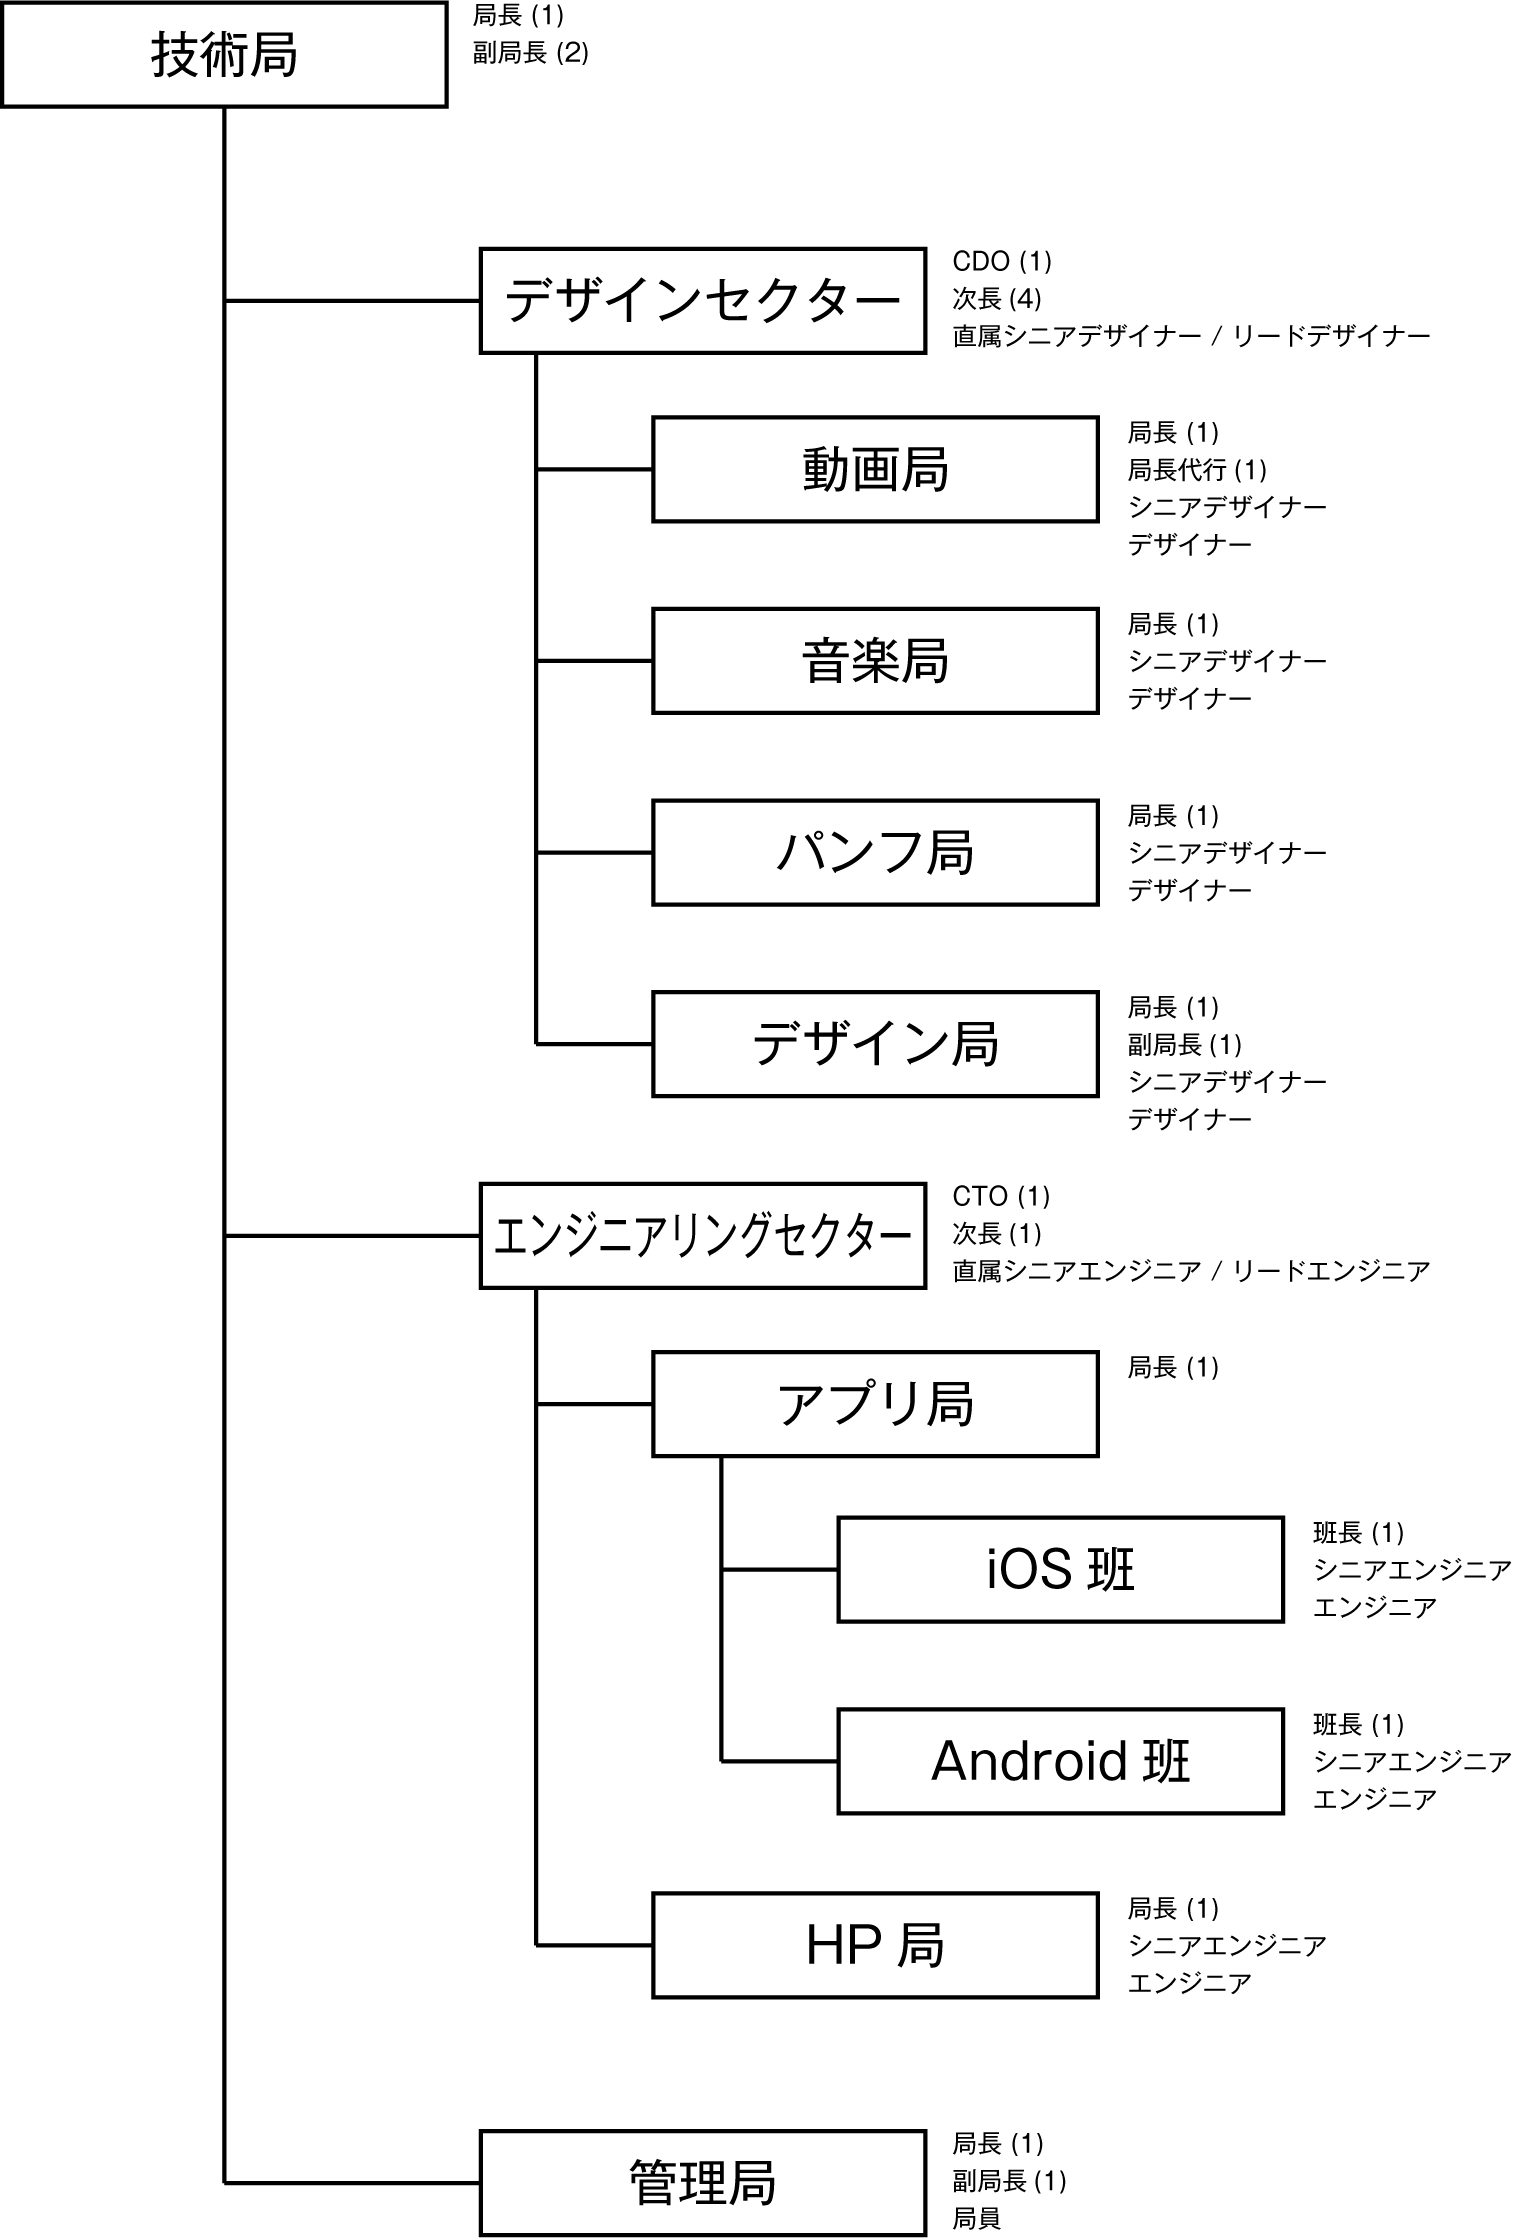
\includegraphics[scale=0.7]{assets/tech.png}\\

\subsubsection{組織}
以下全てにおいて同じですが、上に示した組織形態は60期が決めたものです。君たちがよりよい方法を見つけたらぜひ転換してください。
\begin{itemize}
  \item デザインセクター\\
  内局に4局をもつ。デザインセクターとしては、この4局に振り分けることのできない業務や、この4局に所属しないデザイナーの管理、横断的な業務、デザイン統一等の業務を行う。
  \item エンジニアリングセクター\\
  内局に2局をもつ。エンジニアリングセクターとしては、この2局に振り分けることのできない業務や、この2局に所属しないエンジニアの管理、横断的な業務を行う。特に、統一シフト・QR系のシステム等の開発業務は一切がここに帰属する。
  \item 管理局\\
  名簿作成、書類作成、予算管理、ドライブ(技術局・聖光祭・体育祭・生徒会 etc...)の整理、Slackの整備等の事務(一部技術長・副技術長の事務作業を含む。)を行う。また、技術長・副技術長の事務作業の補佐をする。管理局長の浅井\footnote{60003asai@seiko.ac.jp}が廃止を提言しているので、次期局長の推薦指名は行いません。
  \item 動画局\\
  生徒会、聖光祭、体育祭において、それぞれに関係する各種動画の映像作成・撮影を行う。
  \item 音楽局\\
  動画局の制作する動画の音楽を作るなど、音楽関係の業務を行う。
  \item パンフ局\\
  聖光祭のパンフレットを制作する。生徒会では、DTPデザインを行うこともある。
  \item デザイン局\\
  聖光祭の装飾物のデザインを行う。その他、スローガンロゴのデザイン、アプリ・HP等のUIデザインなども管轄でした(より別のスキルが必要だし、セクターに回してもよい)。生徒会では、選挙広報や外注物のデザインも行っている。パンフ局と協力なりすること。
  \item アプリ局\\
  iOS班とAndroid班に分かれる。それぞれの聖光祭アプリの制作を行う。
  \item HP局\\
  聖光祭HP等の制作を行う。人材不足ですので、次期局長の推薦指名は行いません。次期技術正副部門長で話し合って推薦してください。
\end{itemize}
\subsection{役職と人事、そして自覚}
幹部となったからには、自分の部門の仕事だけしていればいいと思わないでください。全部門の仕事をするつもりでやってください。幹部になるとはそういうことです。人の10倍仕事することを心がけるべし。
\subsubsection{統一}
\begin{itemize}
  \item CDO\\
  デザインセクターの長です。さまざまな分野のデザインに知見がある人で、全体をまとめることができる人がなることが望ましいです。リードデザイナーから一人抜擢すれば良いです。4局に漏れたデザイン業務はここでやります。
  \item デザインセクター直属シニアデザイナー\\
  4局に漏れたデザイナーの局員はここ所属にしましょう。十分スキルとセンスがある人が望ましいです。
  \item リードデザイナー\\
  さまざまな分野のデザインに知見があり仕事ができる人をリードデザイナーとします。大体複数局掛け持ちです。
  \item CTO\\
  エンジニアリングセクターの長です。さまざまな分野のテクノロジーに知見がある人で、全体をまとめることができる人がなることが望ましいです。リードエンジニアから一人抜擢すれば良いです。2局に漏れたシステム業務はここでやります。
  \item リードエンジニア\\
  スキルが高く技術の知見がある人で、仕事ができる人をリードエンジニアとします。大体両局掛け持ちです。
  \item エンジニアリングセクター直属シニアエンジニア\\
  2局に漏れたエンジニアの局員はここ所属にしましょう。十分スキルとセンスがある人が望ましいです。
  \item 各セクターの次長\\
  CDOやCTOに次ぐ人材を入れてください。
  \item デザイナー / エンジニア\\
  各局の局員をデザイナー・エンジニアと呼びます。そのうち技術やセンス、経験が豊富な人をシニアデザイナー・シニアエンジニアとします。
\end{itemize}
\subsubsection{聖光祭}
\begin{itemize}
  \item 技術部門長\\
  拡大実行会議、部門長会議にも出席し、祭全体の梶切りに参加するとともに、それぞれの局の業務を統括します。また実際には、いずれかの(複数の)局の業務を局員として行います。長だからマネージメントに徹して一般スタッフの仕事は行わなくていいというのは大きな間違いです。\footnote{例えば、世界有数の数学の研究所である京都大学数理解析研究所の所長は、歴代フィールズ賞受賞者など、大きな功績を残した数学者が務めています。} 自分自身が貪欲にスキルの勉強をして部門員としても仕事をしてください。また、これは他の幹部も共通ですが、幹部であるという立場として、執行部や他の部門に積極的に切り込んで行って手助けや効率化を行うのは当然です。そして、副部門長をはじめとした多くいる部門幹部に仕事を振り、逆にキャパオーバーぽい幹部(基本全員ですが)を見つけたら程よく手助けするのが肝心な仕事の一つになります。30分睡眠で一ヶ月耐えられる体力とそれでも成績を殺さない学力はつけておくべきです。
 \item 技術副部門長$\times2$\\
  拡大実行会議に出席し、祭全体の梶切りに参加するとともに、担当の局の業務を統括します。青ネク3人それぞれの得意分野を考慮して担当局を振り分けると良いです。また部門長同様、いずれかの(複数の)局の業務を局員として行います。特に今年は、両副部門長とも局長を兼任していました。部門長の補佐をしながら自分の仕事をこなすのは本当に体力がいるので覚悟しましょう。
  \item 各局長などその他の幹部\\
  青ネクではありませんが、拡大実行内でプロジェクトを立ち上げるなど、積極的に祭全体に関わるとともに自分のスキルを最大限活かす方法を考えてください。それぞれの局の業務については他節で記しますので割愛します。
\end{itemize}
\subsubsection{体育祭}
実際の幹部(ピンクT)は以下3人で良いと思います。
\begin{itemize}
  \item 技術局長\\
  週一回から二回の体育祭実行委員会の会議 \footnote{20時半から大体深夜までかかります。} に出席し他の幹部と同様体育祭全体の方針決定に関わるとともに、体育祭全体で技術を使って助けることのできる部分を探していきます。ドライブの管理、名簿の管理、書類の管理などを含みます。当日は運営として走り回ってください。技術部門長と必ずしも同じ人である必要はありませんが \footnote{例えば同じく実行委員会の内局である放送局は放送委員長・放送部門長と異なる人が務めている年「もあります」。} 、まあ長ぐらいは同じでもいいんじゃないでしょうか。
 \item 技術副局長*2\\
  局長とすることはほぼ同じです。当日も走り回ってください。今年は副局長はあんまり会議に来ませんでしたが、できるだけ毎回出席しよう。人事は聖光祭と違くてもいいと思います。
\end{itemize}
\subsubsection{生徒会}
\begin{itemize}
  \item 技術長\\
  技術局の委員会化が公式になされておらず、選挙もしていないので、僕が役員なのかは微妙でしたが、週一回の定例会は毎回でなくとも行くようにしましょう。
\end{itemize}
\subsection{人物}
60期を中心に何をしていた人なのかを逆引きで書いておきます。なお、特記がない場合は生徒会とは第35期生徒会を、聖光祭とは第62回聖光祭を、体育祭とは第36回体育祭を指します。また、特記がない役職は生徒会・聖光祭・体育祭共通の人事です。
\subsubsection{技術}
\begin{itemize}
  \item 飼沼\\
  生徒会技術長。聖光祭技術部門長。体育祭技術局長。CDO、リードデザイナー。シニアデザイナー(デザインセクター、動画局、パンフ局、デザイン局)。動画局長代行。シニアエンジニア(エンジニアリングセクター)。第61回聖光祭総技研副所長・動画局長・パンフ副局長、統一シフトプロジェクトマネージャー。体育祭青組応援団。情報公開における書類の書式統一等に関する小委員会・書紀班 総書記、議長(Tシャツ発注関係小委員会)、議長代行副議長(新型コロナウイルス感染症対策小委員会)、副議長(電子マネー等導入小委員会、食品アレルゲン等表示小委員会、情報公開及び聖光祭実行委員会細則制定に関する小委員会、動画撮影等小委員会、震災対策関係小委員会、舞台演出関係小委員会(Production Designer))、委員(YouTube配信関係小委員会、グランドフィナーレ関係小委員会、統一シフト関係小委員会、オンライン食品予約システム関係小委員会、事前予約関係小委員会、アンブレラスカイ関係小委員会(設置図設計)、トレジャーハント関係小委員会(UI)、サインデザイン関係小委員会(企画)、アプリ使用決定関係小委員会(UI)、展示団体等管理小委員会(スタッフ))など。\\
  <略歴>2018/1 外務部門総技研動画局入局。2018/12 装飾部門デザイン課入局。2019/1 外務部門パンフ局入局。2019/5/1 パンフ副局長。2019/5/2 総技研動画局長。2019/5/28 総技研副所長。2020/9 情報技術統括所副所長。\\
  <部門長コメント>幹部、部門員としての仕事に加えてダンス(ステージ、グラフィナ、閉会式、ゲリダン)や演奏(弦オケ、合同、グラフィナ)もいろんなことに手を出しすぎてたかもしれません。まあ頼まれた仕事は断らない方がいいですよ。当日までは限界を超えなくていいので限界をあげる努力をするといいと思います。
  \item 李\\
  聖光祭技術副部門長。体育祭技術副局長。生徒会監査副委員長(DX)。CTO、リードエンジニア。シニアエンジニア(エンジニアリングセクター、アプリ局iOS班、Android班、HP局)。HP局長。シニアデザイナー(デザインセクター;UI)。アプリ局iOS班長。第61回聖光祭アプリ局長、統一シフトリードエンジニア、第62回聖光祭QRコードシステムリードエンジニア(バックエンド、フロントエンド)。情報公開における書類の書式統一等に関する小委員会・書紀班 総書記、議長(統一シフト関係小委員会)、副議長(電子マネー等導入小委員会、食品アレルゲン等表示小委員会、情報公開及び聖光祭実行委員会細則制定に関する小委員会、オンライン食品予約システム関係小委員会、事前予約関係小委員会、トレジャーハント関係小委員会、震災対策関係小委員会、アプリ使用決定関係小委員会)、委員(舞台演出関係小委員会、展示団体等管理小委員会(スタッフ))など。\\
  <略歴>2018/1 外務部門総技研動画局入局。2018/9 外務部門総技研アプリ局入局。2019/5/2 総技研アプリ局長。\\
  <部門長コメント>彼は超有能でした。言わずもがなですが。何でもできるので何でもやってました。かつずっとする根性のある人。(仕事)=(有能さ)*(仕事時間)
  \item 浅井\\
  生徒会副技術長。聖光祭技術副部門長。体育祭技術副局長。リードデザイナー。シニアデザイナー(デザインセクター、動画局、パンフ局、デザイン局)。管理局長。外務上がり。体育祭緑組応援団。情報公開における書類の書式統一等に関する小委員会・書紀班 総書記、副議長(Tシャツ発注関係小委員会、電子マネー等導入小委員会、食品アレルゲン等表示小委員会、情報公開及び聖光祭実行委員会細則制定に関する小委員会、震災対策関係小委員会、舞台演出関係小委員会、アンブレラスカイ関係小委員会)など。\\
  <部門長コメント>彼は頼まれた仕事を絶対に断らない人です。たくさん仕事を投げましたが、断られたことは一度もないです。勝手に右腕だと思ってました。
  \item 鈴木\\
  生徒会デザイン局長。聖光祭装飾副部門長、デザイン副局長。体育祭デザイン局長。デザインセクター次長、リードデザイナー。シニアデザイナー(デザインセクター、動画局、デザイン局)。体育祭黄組応援団デザインチーフ。\\
  <略歴>2019/3 装飾部門デザイン課入局。2019/7 外務部門総技研動画局入局。\\
  <部門長コメント>デザイン関係なんでもできる装飾のベテランです。動画もCGもやってくれました。まじでどうしてそんなに仕事量こなせるのかわからない人の一人です。
  \item 黒羽\\
  デザインセクター次長、リードデザイナー。シニアデザイナー(デザインセクター、パンフ局、デザイン局)。パンフ局長。体育祭白組応援団。\\
  <略歴>2019/5 外務部門パンフ局・装飾部門デザイン課入局。\\
  <部門長コメント>めっちゃセンスある。パンフはほんとに仕事の量が多いのでやりきれたのは彼の力量です。あと細かい雑用めっちゃやってくれた。
  \item 三枝\\
  デザインセクター次長、リードデザイナー。シニアデザイナー(デザインセクター、動画局、パンフ局)。動画局長。シニアエンジニア(エンジニアリングセクター、アプリ局iOS班)。\\
  <略歴>2018/3 外務部門総技研動画局入局。\\
  <部門長コメント>多分動画局の仕事以外の方がしてます。生徒会室で作業していた時間とその幅は青ネクレベルでした。
  \item 満田\\
  シニアデザイナー(音楽局)。音楽局長。\\
  <略歴>2019/1 外務部門総技研動画局入局。\\
  <部門長コメント>グラフィナのステマネ決めたり音楽曲の仕事の幅を最大限に広げてくれました。
  \item 矢向\\
  シニアエンジニア(エンジニアリングセクター、アプリ局Android班)。アプリ局長。\\
  <部門長コメント>仕事早すぎてUI担当の僕の仕事が追いついてなかった。李が育てた有能です。
  \item 鬼頭\\
  シニアデザイナー(デザインセクター;CG)。シニアエンジニア(エンジニアリングセクター、アプリ局Android班)。美化部門現場統括。体育祭赤組応援団デザインチーフ。\\
  <部門長コメント>何でもしてくれた。美化のみなし幹部にも関わらずCGのプロ。
\end{itemize}
\subsubsection{その他}
\begin{itemize}
  \item 大下\\
  聖光祭実行委員長。シニアデザイナー(パンフ局、デザイン局)。管理局員。第61回聖光祭副実行委員長。体育祭青組大将。技術局員の実行委員長という前代未聞。\\
  <部門長コメント>
  \item 古澤\\
  聖光祭副実行委員長。シニアデザイナー(パンフ局)。なぜかGASを30分で修得して書いたりしてた化け物です。体育祭青組応援団。技術の仕事をたくさん肩代わりしてくれました。
\end{itemize}
\subsection{教職員}
関係する教職員を逆引きで示す。以下は全て2021年度のもの。学校は会社同様、年度で人事も全て刷新される(変更がある可能性も大いにある)。
\subsubsection{事務職}
\begin{itemize}
  \item 事務室\\
  忙しいので早めに連絡すべし。生徒があんまり好きじゃないので、伝達は簡潔に、仕事は早く、話す内容は用意してから。
  \item 野口 周作 さん(事務室)\\
  事務長。多分関わるのはだいたいこの人。Adobeの管轄。資材の管轄でもある。
  \item 吉岡 敏子 さん(校長室)\\
  校長秘書。教員の悪口を言いがち。校長先生にface-to-faceの用があるときは必ず吉岡さん経由でアポを取る。
\end{itemize}
\subsubsection{教職}
情熱がある先生、生徒を大事にしてくれる先生がほとんどですが、それでも大人。教職も忙しいですし、面倒なことは断られやすいです。その上でどう通すかを考えよう。
\begin{itemize}
  \item 職員会議\\
  職員の会議は木曜日(多分)。また、毎朝8:10〜朝礼で教務主任の小泉先生が全先生に連絡事項を伝達します。HRでの伝達は担当先生経由で小泉先生にお願いしよう。ちゃんと聞いてない先生や忘れる先生もいるので、その誤差に注意。

  \item 生徒指導部\\
  飯岡先生、石渡先生、滝本先生、川部先生、等々がいることしかわかりませんが、企画書等はここで審議されます。急ぎのものがあっても、生徒指導部の会議は金曜(変更になっている可能性があるので先生に確認のこと、4月では多分変わります)4限で固定なので、これを待たなければいけません。

  \item 飯岡 雄介 先生\\
  聖光祭顧問。執行部顧問。理科科(化学)。S3D担任。バレー部顧問。少し厳つい先生ですが、だいたい優しいです。キレると少し怖いです。

  62回では高3の担任をしながら聖光祭の顧問をやるという過労。飯岡先生のやることは超多いので、迷惑や心配をかけないように。飯岡先生と仲良くなると色々うまく回ります。部門顧問をかっ飛ばして飯岡先生に相談するのも度を過ぎなければよいです。早寝早起きです。月曜研修。

  \item 石渡 巧 先生\\
  生徒会顧問。執行部顧問。社会科(世界史)。S3C担任。陸上部主任顧問。だいたい優しいですが、問題発言をする癖があります。本人のいないところで陰口を行ったり、僕が欠席した予算審議で技術局の悪口を言ったりしてました。

  それと、基本的に全てを忘れています。自分で決済した物品も1週間後には何も覚えていません。それを考慮して動かないとひどい目に遭います。石渡先生も忙しい方ですので、早めに相談しよう。木曜研修。

  \item 川部 大輔 先生\\
  体育祭顧問。聖光祭企画/演出顧問。体育科。S1E副担任。バレー部主任顧問。面倒です。基本は優しいですが、生徒を小馬鹿にしています。一度話し始めると長いです。話すのは最小限にすべく、川部先生の追及を受けることがないようにしよう。ブチギレると体罰もします。土曜研修。

  以下、バレー部長李からのアドバイス。会話の回数と長さは反比例するので長い話をたまにするか、短い話をちょくちょくするかを選びましょう。なんなら自分はじぶんから話しかけ、わかりきってることを何回も確認しました。もし本書を読んでいるあなたがそんなに高い役職じゃなければ高い役職を間に入れて身代わりにして連絡を取るようにしましょう。

  \item 宇佐美 直也 先生\\
  技術部門顧問。理科主任(生物)。S2D副担任。生物部主任顧問。\\
  2021年度技術部門顧問。\\
  基本的に``めんどいからやりたくない、だけど金が貰えるからやってやる''が座右の銘。
  \textit{Digital Detox}をしてました。仕事放棄してたくせにあとからブチギレてきた。だいぶ心に傷を負った上この人のせいでできないことも多くなってしまったので、早めに事前報告/相談しておくといいよ。

  \item 山口 ゆり 先生\\
   情報科。\\
   神教員。IT系で相談があればまずは山口先生に相談すべし。自動的に宇佐美先生にも話がいくので非常に楽。全力を尽くして対応してくれる。
   ごくごくたまに、機嫌が悪いとき、怪文書をメールで送ってくる。

  \item 河野 周 先生\\
  英語科。S2B担任。硬式テニス部顧問。\\
  2020年度技術部門顧問。\\
  神。生徒を信頼しているので、危険なことをしなければ、先生が学校にいなくても活動を許可してくれる。2021年3月に、コロナ禍で部活動禁止ても、動画局の撮影を特別に活動を許可してくださった。

  \item 百武 沙紀 先生\\
  英語科(帰国英語)。PiTの顧問で、技術系に理解があります。何らかの形で関われるといいかも。

  \item 神保 元 先生\\
  国語科(現在は古典)。J2C副担任。コンピュータ部副顧問。講堂担当。

  優しい。全力で対応してくれる。講堂の映像音響関係は相談すべき。

  \item 小泉 直範 先生\\
  教務主任。数学科。基本は優しいです。

  \item 花家 徹 先生\\
  副校長。社会科(現代社会家庭、現在は特別科目のみ)。生徒の安全に関わる最低限のラインを守ってくれるベテラン。

  \item 滝本 和彦 先生\\
  体育科。執行部顧問。考え方が古い。

  \item 松原 宏樹 先生\\
  社会科(地理)。講堂担当。講堂の件は放送通じて早めに相談。

  \item 出口 義則 先生\\
  数学科。東京大学数学科卒の変人。聖光生に理解がある。聖光祭に理解がある。講堂担当。
  \\口癖:「ちょーだいね」
  「ちゃんとやっといてちょーだいね。」を言いがち。\\
  無賃金強制労働させられているため、事前に申告したこと以外のことをやると怒られる。\\
  講堂のステージ上で飲み物を飲むと怒られる(当たり前)。\\
  加えて、結構口出ししてくる。適度に流して活動に集中しよう。

  \item 工藤 誠一 先生\\
  校長。社会科(政治経済公民、現在は教職なし)。

  神。iPad20台の交渉も一瞬で許可してくださった。技術部門の設立はこの人の鶴の一声です。

  予算で落ちないけど欲しいものがあったら工藤校長に要相談。全ての工程をスキップして購入許可が降りる。ただこの手法をやりすぎると生徒指導部の反感を買います。

  たまに校長から直接依頼が来ます。新所長は挨拶しておいてね。
\end{itemize}

\subsection{立場と名称}
\subsubsection{生徒会}
59期の齋藤先輩が「情報技術統括所」(略称:「ITEC」)という謎名称をつけてしまったところ、「総合技術研究所」「技術局」の名前と混乱され多分俺らしかわかってない。近い人には「情技統」「情統」「ITEC」の名前で呼ばれる。僕(飼沼)はGTECっぽくてあんまり好きじゃないので、「技術局」(役職の場合は「正副技術長」)を使いがちです。第35期生徒会役員会において委員会化が全会一致で可決し、オンライン投票の試験運用として委員会化の全校投票および首長の選挙が行われる予定であったが、スケジュールが合わず不可能となった。委員会化は可決しているので、次年度も役員会で過半数(賛否同数の場合は生徒会長の決定による)の反対がない場合は、委員会化投票の手続きを進めても問題ないであろう。「技術局」は事務局・会計局と混同される恐れ、「技術委員会」は怪しそう、等々の意見があったので、次年度の解決に委ねます。
\subsubsection{聖光祭}
第62回聖光祭にて部門独立。飯岡先生に大下から無理を言って幹部の人数を申請したので、これ以上増やすとなるとさらに交渉が必要か。基本的に教員に煙たがれていることを理解し、お取り潰しなどないよう、{\bf 期限などは絶対守るように行動}すること。
\subsubsection{体育祭}
第35回体育祭にて技術課として設置。第36回体育祭にて技術局(放送局・新設の装飾局とともに実行委員会内局)となる。

\subsection{予算}\label{sec:予算}
\subsubsection{減価償却}
59期の齋藤所長は総額100万円の買い物をするために例年減価償却と言う形で後輩の予算を使うことを決定しました。何も覚えていない石渡先生は自分で許可したにも関わらず一年後にブチギレてましたが、以降こんな方法を使うのはやめましょう。本来減価償却とは、企業等で耐用年数を一年として計算しては割りが合わない会計上の物品を法律に則った年数で処理するものですが、この減価償却予算は色んなものが適当に長めの年数で教員と役員の目を騙すために組まれています。

申し訳ないことこの上ないですが、{\bf 資料内のスプレッドシートに従って約22万円を生徒会予算に計上してください}。石渡先生はどうせ忘れていらっしゃって文句を言われるので、経緯を説明しましょう。なお、ドローンについては、航空法によって指定される政令の改正によって運用が難しくなり、生徒指導部会議で却下されました。

\subsubsection{生徒会予算審議}
技術局は通年を通して使えるものは基本的に生徒会予算で落とします。3学期始業式ごろに第1次予算審議が開催されるので、それまでに予算案を用意しよう。期限厳守、会計局長の提示したルール厳守。

購入する物品名、単価、個数、小計、物品の用途、総計、昨年度との違い、作成年月日(更新のたびに書き換える)を明記しよう。

会計がポンコツな年は小計を手動で計算させてたりするので指摘しよう。スプレッドシートの形式のおすすめは、マイナスかっこの会計フォーマット(¥ (1,000.12))を「小数点以下の桁数を減らす」で整数値にしたもの。

資料に今年の予算を貼りました。

\subsubsection{聖光祭予算審議}
3学期の初めに第1次、終わりに第2次、(例年は)1学期の初めに第3次があります。聖光祭にのみ関連する物品はこちらで買ってもよいでしょう。なお、{\bf パンフ・ポスターの発注予算については外務・執行部と管轄を相談してください}。

部門長と実行委員長、会計幹部、飯岡先生、石渡先生が出席します(副実行が予算を把握してなくて困ったので、副実行も出席にした方がいいかもしれません)。あくまで予算審議なので、予算報告会にならないようみんなで議論する場にしよう。

第3次予算審議以降は基本的に予算を変更することはできません。適当にやると後で後悔するのでしっかり練ってこよう。

今年は使いすぎました。ごめんなさい。また、装飾がアンブレラスカイの巨額予算を執行後にもってくるという前代未聞の事態が発生。推し企画だったし成功したので文句は言わなかったですが、こういうことはない方がいいです。

\subsubsection{運用}
ちゃんとスプレッドシートを使ってもう執行したものを記録するようにしてください。こんがらがります。また、プロジェクトの担当をやっていると部門横断で金銭管理させられることがあります(ex. 撮影、プリンター、コロナ対策等)。それぞれ管轄とかを記録できるスプレッドシートを作ろう。

そして、領収書、前払いの場合の金銭をなくさないように。まあ心配ないと思いますが...

経費は前払・後払・振込のいずれかの方法によります。振込は石渡先生が所持する生徒会のクレジットカードで行うので石渡先生の執行許可が必要です。

いずれも会計幹部に相談してから執行を行うようにしましょう。資料欄にある経費申告書をボールペンで記入し、領収書を裏に添付して会計に渡します。学校の金庫の価格が不足している場合は会計幹部が銀行からおろしてくるのを待つ必要がありますので、早めに相談しましょう。今年は当日に20万円必要になって忙しなくなりました。封筒に価格と責任者、管轄(複数の場合は全て)、用途をボールペンで明記しよう。

また、振込で行うと先生を通す必要があり、予算の解釈を厳しくされてしまうので会計幹部を通すことがいいと思います(今年は感染対策関連の予算で、金額空白であった管理予算や「資材用」とのみあった食品予算を用いました)。なお、予算審議前に物品購入をするためには会計と先生の許可が必要ですので、相談しましょう。

物品を学校に発送するときは、受付の方に伝える必要があります(今年は専用の書類を作りました。執行部管轄ですので、執行部に早めに確認してください)。代引の場合は金銭を預ける必要があります。任命式で飯岡先生に資料をいただくと思いますので、確認してください。

\subsubsection{決算}
聖光祭が終わった後も、体育祭・生徒会のみならず聖光祭の決算処理は続きます。会計は聖光祭が終わってもずっと処理です。リスペクトを忘れずに、迷惑をかけないようにしよう。ていうか普通にちゃんとまとめとかないと会計のみならず自分たちも面倒なことになります(今なってます)。

\subsubsection{資料}
\begin{itemize}
  \item \href{https://docs.google.com/spreadsheets/d/1cCHlfuN5FRR4mlCLDqwohB5WyJ2stmBoUM762DVa7aM/edit##gid=848718781}{技術局統合予算 - 先代が残した減価償却【静】(S)}
  \\ 技術局・技術部門の予算・決算についてはこちら他シートにまとめてあるので確認してください。決算は決算終了時に更新します。また、体育祭では金銭は使っていません。
  \item \href{https://docs.google.com/spreadsheets/d/1Tg_4jKLywMSQpIjNebaPKgTH9YmPqoLZAOGBRs1sr7I/edit?usp=sharing}{第62回聖光祭 第三次予算フォーム (S)}
  \item \href{https://docs.google.com/spreadsheets/d/1zZcA076Hvox9dDIvhHAMnmiIAQI0af1ChN1slH4WyVw/edit?usp=sharing}{第35期生徒会 第二次予算案 (S)}
  \item \href{https://docs.google.com/spreadsheets/d/1uNOAvcq1S3ErZTklh8G7kT6zPYlna-8pR9Jqv2RYYKc/edit?usp=sharing}{第35期生徒会 第一次予算案 (S)}
  \item \href{https://docs.google.com/document/d/1hR_gEl9qHiXGgSxzFDBNH7U6hyPKhjvPEHOStIhGmo8/edit?usp=sharing}{62nd 聖光祭 第1次予算審議議事録 (D)}
  \item \href{https://docs.google.com/document/d/1brt8Fwv7bYzFQlV_zTF3Tmtmhg8zD4gGt-oBMQM-7Iw/edit?usp=sharing}{R2/統括所予算説明資料 (D)}
  \item \href{https://docs.google.com/spreadsheets/d/1tlZiJdgfzjbsGDRE5cx0bnHmj2DNoOukDPuPQMx2N5g/edit?usp=sharing}{撮影機材予算 (S)}
  \\検討段階のもの。技術予算ではありません。
  \item \href{https://docs.google.com/spreadsheets/d/1-HWo9Lh8epNt7tHbg88feTvWC146bmrN0XXh0YFmPzU/edit?usp=sharing}{プリンタ購入予算 (S)}
  \\検討段階のもの。技術予算ではありません。
  \item \href{https://drive.google.com/file/d/1TN5O2NX7dg8xD_-Y-93Du-caYc1XWezX/view?usp=sharing}{経費申告書 (B5 pdf)}
  \item 他なぜか5年前の外務予算とか装飾予算とか持ってたりします。欲しいものあったら連絡してください。
\end{itemize}


\subsection{ハードウエア}
\subsubsection{生徒会管轄}
 現在生徒会で所有している機材は以下の通りである。
 \begin{itemize}
  \item BlackmagicDesign Pocket Cinema Camera 4K\\
  広報委員会が生徒会予算で購入している。
  \item DJI RSC2\\
  カメラ用ジンバル。動画のプロジェクトで必要な機材として、工藤校長先生に購入していただいた。
  \item グリーンバック\\
  使おうと思って購入したが、結局使っていない。ぜひ使って欲しい。
  \item Windows Desktop PC (自作)\\
 40万くらいかけて自作したPC。CGのレンダリングに最適。
  \item Square\\
  9台ある。
 \end{itemize}

 \subsubsection{学校管轄}
 学校側が所有しているが我々が使用できる機材。
 \begin{itemize}
  \item iPad (第八世代)\\
  20台を学校が所有している。\\
  使用する際は情報科の\mail{山口ゆり先生}{yuri.yamaguchi@seiko.ac.jp}に頼むこと。
  \item RODE Wireless Go\UTF{2161}\\
  ワイヤレスマイク。送信機二つと、受信機一つ、3.5mmイヤホンジャックケーブル、ピンマイクが含まれる。使用する際は事務局長の\mail{野口先生}{noguchi@seiko.ac.jp}まであらかじめメールで連絡し、事務室に取りに行くこと。返却する際もあらかじめメールが必要。
 \end{itemize}

 \subsection{ソフトウエア}
 \subsubsection{パスワード関連}
 各種パスワード等は村山、紙田、河原にスプレッドシートを共有します。

\subsubsection{メアド}
生徒会アドレスは生徒会長引き継ぎによってください。聖光祭アドレスは変える方がいいと思います。アドレスに62って入ってるので。一年前の執行部引き継ぎには部門アドレス作れとか書いてあるけどいるのかな?今年はありませんでした。話し合ってみて。

注意点はみっつ。
\begin{enumerate}
  \item メールは日本語に自信のあるやつがかけ。普通にその辺の聖光生は敬語間違ってます。せめて校正サイト\footnote{ex. \href{https://so-zou.jp/web-app/text/proofreading/}{文書校正ツール}}とか通せよ。
  \item 組織アドレスのメール受信については、未読に戻すようにしよう。見逃して大変なことになります。
  \item メール対応は死ぬほどめんどくさいから事前に気をつけよう。
\end{enumerate}

\section{概括}
\subsection{スケジュール}
\subsubsection{選挙まで}
任命式までは幹部としての資格はないことに注意。ただ拡大実行など会議は積極的にやったほうがいいと思います(62回の場合は 2020/5 第一回拡大実行、9 第二回拡大実行、 11 第三回拡大実行、 12初旬 規則関係会議、12中旬 第四回拡大実行 など)。引き継ぎが死ぬほど大変だったので、この頃から毎日日記を書いてると楽かも。

\subsubsection{選挙あと}
幹部名簿は作り始めましょう。こういうのは技術が先導してください。実行委員長が後に飯岡先生から提出用のシートを渡されるので、青ネクのみとピンクTまでを両方作るべきかと思います。学年/クラス/出席番号/学籍番号/メール(以上は統合名簿からvlookupでどうにかできます)/誕生日(ふりふら登録用)/掛け持ち予定 を記録しよう。

\subsubsection{副実行委員長面接}
実行委員長を助けてください。募集の資料を作成し、Classroomで中3/高1に配信。高2副を決めた後、高2副全員で高1副の面接。多少の助言はありだと思います。副実行委員長が誰かは本当に大切です。君らの命綱です。また、{\bf \ref{sec:議事録班}} にも書きますが、面接の発言録をとってください。

\subsubsection{初回オフライン拡大実行}
幹部が全員確定した時点で拡大実行を行って全員で顔合わせをしよう。ふりふらの団体登録(もうしてあるかな?)を済ませ、全員でLINEスケジュールなどで予定調整し一研を早めに予約しよう。初回ではお世話になるふりふらの方を呼び入れて全員で挨拶すること。反省点の洗い出しと新しくやりたい企画などについて話すといいと思います。

\subsubsection{任命式}
毎年、2学期期末試験最終日に飯岡先生から聖光祭幹部に聖光祭活動に当たっての諸注意があります。この任命式を以て、内定している聖光祭幹部が学校側として正式に認められることになります。この日以降は、聖光祭活動が正式に認められます。任命式終了後は幹部全員で顧問教諭に挨拶しにいきましょう。

\subsubsection{冬休み}
冬休みは全て聖光祭に捧げるくらいでいきましょう。執行部に確認し、活動予定表を埋める必要があれば期限厳守で提出すること。特に撮影などをしたい場合は顧問教諭と飯岡先生両方に確認を取りましょう。また、全部門で倉庫(41等)の整理をするといいと思います。管轄を決め物品を全てスプレッドシートに書き出しましょう。Tシャツ関連の動き出しを忘れずに。

\subsubsection{部門ガイダンス}
1月に行われる部門ガイダンスの資料作成をしてください。冬休み明けにすぐに先生方の校閲を受け、生徒会室の画鋲を使って幹部全員で協力して各教室の後ろにガイダンス資料を貼りましょう。中学1年生を放課後小講堂に集めて各部門長から各部門の紹介をします。紹介するためのスライド、手元でも各部門の仕事が確認できるよう部門ガイダンス資料を作成しておこう。スライド原案は各部門が作りますが、デザイン統一は技術がやってください。発表する際は、腕章を忘れずに、身なりも整えてくること。印刷は聖光祭執行部経由で頼みましょう。

部門紹介用の紙を各クラスに貼ってもいいんじゃないでしょうか。例年はやっていた気がします。


\subsubsection{部門動向調査}
仮(動向把握、各部門過不足を確認する)、本(基本確定)がある。制限に従ってフォームを作り、回答のスプレッドシート記録をONにし、さらにそれを用いて処理用スプレッドシートを作る。{\bf \ref{sec:統一シフト-部門動向調査}} 参照。当日、全幹部で教室に赴き、これらをわかりやすく説明する。ただし、事前に担任の先生に担当が挨拶をしてから行くこと。幹部が理解していないと死ぬほどグダリます。全幹部でコンセンサスをとれ。

\subsubsection{第一次予算審議}
{\bf \ref{sec:予算}} を参照。

\subsubsection{第一回チーフ集会}\label{sec:第一回チーフ集会}
\subsubsubsection{いろは作成}
この頃に展示部門のいろはの連絡が来るので、記入しよう。パンフ局・アプリ局・HP局は素材提出時の注意について、デザイン局は装飾と相談してデザインチェック関連について書けばいいと思います。いろはについては展示の引継を参照してください。

\subsubsubsection{素材表}
パンフ局・アプリ局・HP局で合同の素材提出表を作って、展示・食品に渡してチーフ・店長に見てもらおう。展示部門経由・食品部門経由でやるかは任せます。昨年はドライブに入れさせる方法を取りました。

これ死ぬほど多いです。局長三人と技術幹部+執行部複数人でやろう。部門の分もこの時期につくるのをお勧めします。団体チーフとかからは複数に提出するのはストレスなので、最小公倍数を取って出してあげよう。そんで部門の中にも出さないやつらはいます。期限は2段階早めに設定しリマインドせよ。

\subsubsubsection{資料}
\begin{itemize}
  \item \href{https://docs.google.com/spreadsheets/d/1CQqoQk9K2541dx-WhdyMl7i6m3l4NQxOgOrnMKgY9Eg/edit?usp=sharing}{第61回パンフ局 4月開催予定時のワークフロー (S)}
  \item \href{https://docs.google.com/spreadsheets/d/1_B39iTxYG4pPTYhmjbtjTS1wA9dnm_Zg4s-35IgFcXM/edit?usp=sharing}{第61回パンフ局 実際のワークフロー (S)}
  \item \href{https://docs.google.com/spreadsheets/d/1NF84N6ftFbk_4xFw5B_V4LpxlGhZCpm0oSgIBLLYLrs/edit?usp=sharing}{第62回統合素材表 (S)}
  \\ これ統合できてないかもしれない。すまない。同じフォルダに素材表全て入ってます。
  \item \href{https://docs.google.com/spreadsheets/d/1-toba1DrCHhMQ5el9HqFxUu-kmNuYwbTGwxs1x6KUWQ/edit?usp=sharing}{62nd聖光祭 パンフ用素材一覧 (S)}
  \\ これが最新か...?
\end{itemize}

\subsubsection{局の仕事}
三学期に入って本格化します。余裕こいてると痛い目に遭います。もうこれはやるしかないです。正副部門長は進捗確認というか自分がやるぐらいの心算でいないと終わらないですよ。

\subsubsection{春休み}
春休みは聖光祭です。長期休暇は毎日来るのは当たり前ですが、始発で学校に来る $\longrightarrow$ 学校で作業 $\longrightarrow$ ふりふら $\longrightarrow$ 日付が変わるまで外で作業(ふりふらが20時閉館の時代だったので) の繰り返しとかいう地獄みたいな日も多くありました。日によっては十個以上の会議が入って朝の3時まで続いたりとかも... 遅寝早起きができるようになっておいた方がいいです。それと、Googleカレンダーとかをうまく使って予定管理しないと会議がクアドルプルブッキングしたりします。

以下やらなきゃいけないことは書ききれないほど多いですし書いたとしても何倍にも膨れあがること間違いなしなので逐一は書きません。

\subsubsection{準備日}
カタカナ教室に本部ができます。始発で来て本部一番乗りしよう!各種設営、入場システム関連がある場合には準備、幹部シフト確定、Tシャツ配布などなど。机移動というビッグイベントもあります。机移動中はBuddycomを机移動以外の話題通常連絡禁止がいいかと。
今年は本部を四教室つくりました。客から見える教室には模造紙(本部マタイには蛇腹と看板をおこう。管轄は執行部から飯岡先生ですが忙しすぎて忘れていることも多いのでなかったら早めに。今年は管理がやってくれました)を貼って支部と示すための張り紙を貼るべし。なお、外務 (手荷物預かり所J3E/本部J2UT)・美化 (サスペ奥)・会計 (職員室内小会議室)・管理 (ルーフガーデン前・準備日のみ) などは本部を持ってます。
\begin{itemize}
  \item ヨハネ $\cdots$ 実行支部+技術本部+ラミネート本部+Tシャツ配布本部
  \item マタイ $\cdots$ 実行本部+執行部本部+展示本部
  \item マルコ $\cdots$ 実行支部+感染対策本部+企画本部+パンフ挟み込み本部
  \item ルカ $\cdots$ 実行支部+感染対策支部+装飾本部 (準備日のみ)
\end{itemize}

\subsubsection{当日}
やばいです。連携が不可欠。僕(飼沼)や李、韮沢(管理副部門長)、黒羽は前泊しました。大下・永井(外務幹部)とかは二泊してたと思います。事前に執行部と一緒に各部門の動き方のタイミングについてマニュアルを作ろう。特にグラフィナ予約時、グラフィナ前をはじめとして、講堂棟の誘導は聖堂・2回席まで含めて動線を事前に会議して定めておかないとカオスです。幹部シフトをきちんと組んで誘導人員をしっかり確保しよう。

\subsubsection{片付け日}
とにかく時間がない。死ぬ気で片付けよう。音楽・動画局はED、他閉会式準備。

\subsubsection{以降}
引き継ぎ(これまで引き継ぎもらったことがなかったからなんですが、一から引き継ぎを作って死ぬほど時間かかりました)と決算かな。打ち上げは楽しんでね。僕(飼沼)は今年携帯と財布を忘れた状態で3次会後に終電で北浦和まで寝過ごすひどい目に遭いました。

\subsection{各部門との連携}
聖光祭で大事なのは幹部間の情報共有です。お互いに何の仕事をしているのか共有し、開放感のある雰囲気を作り、拡大実行全体で一体となって行動しよう。さもなくば聖光祭は失敗します。部門によっては、幹部候補生や幹部補佐(食品)、統括みなし幹部(美化、放送)、チーフ・サブチーフ(企画)とか置いてるとこもあります。幹部名簿に加えてこういう人たちも名前と顔を覚えておくぐらいの心算でいないとだね。全幹部と仕事しよう。

\subsubsection{執行部}
執行部は全てを取りまとめるところ。だからこそ、失敗を怒られもするし、逆にサボっていたら怒るのが正しいです。ただ、執行部は本当に忙しいです。時に部門の仕事をたっぷり肩代わりしたり、相当な責任を背負っていたりします。感謝と思いやりを持って接し、仲良くしよう。

執行部はやることが漠然と(「サポート」「取りまとめ」)していますし、タスクが積み重なっている忙しい部署ので、執行部全体に頼んでもヘルプが帰ってこないのは茶飯事です。こちら側から直接メンションし、「担当は〜でいい?」「〜までに〜をやるのを手伝って欲しい」とお願いしよう。高一にも。どんなに忙しくてもコミュニケーションをサボるのはだめです。

何かあったらすぐに執行部に相談しよう。執行部と相談して進めるのが一番大事です。また、執行部が死にそうな時は、積極的に仕事を手伝おう。技術部門の鉄則:「自分が執行部であるかのように行動しよう。」

飯岡先生や石渡先生と話がしたい時は、執行部に仲介してもらうか、一緒に職員室に伺うのがよいです。

\subsubsection{演出部門}\label{sec:演出部門}
演出部門はバンドを統括するところ。一方で、グラフィナなどの舞台演出の仕事を企画部門とともに担当します。ですから、動画局・音楽局は積極的に演出とコンタクトを取りましょう。講堂関係なども、全体でコンセンサスが取れている状態で教員と交渉しよう。ライブハウスの装飾をやってあげることになるかも。\\
{\bf 注} バンド掛け持ち幹部の演出の所属有無について決めておこう。後々名簿に追加する事になると面倒です。

\subsubsection{外務部門}
外務部門は対外関係全てを統括するところ。いっつも仕事部門です。入場関係のシステムでは外務ときちんと調整しよう。

また、ポスターとパンフの入稿関連の管轄を事前に決めてください。パンフの広告は外務が担当しますが、ポスター・パンフの入稿作業は執行部がやるのか?技術がやるのか?外務がやるのか?仕事の忙しさによっては管轄を変更しよう。外務は細々とした作業がずっとあります。連絡が遅くなると本当に迷惑をかけますので、注意してね。

送付状の差込についてはGASで自動化してあげてください。{\bf \ref{sec:外務送付状の差込}} 参照。

\subsubsection{装飾部門}
装飾部門は装飾物関係を全て統括するところ。デザイン局には装飾上がりの人も多いかと思います。デザイン局と装飾部門の連携はしっかりとること。また、サスペの借用関連、垂れ幕関連等では装飾・展示・食品間等で話し合いがあると思いますので注意。

\subsubsection{企画部門}
企画部門は聖光祭の企画関係を統括するところ。スステージ企画課、春夜祭課、誘導課があります。さらにグラフィナを監督します。やること多すぎ部門です。
グラフィナの企画・舞台演出などを担当しますから、動画局・音楽局は積極的に企画とコンタクトを取りましょう。閉会式などの舞台演出も行うのであれば手伝ってもらってもいいと思います。他誘導などについても {\bf \ref{sec:グラフィナ}} を参照のこと。

\subsubsection{食品部門}
食品部門は聖光祭の飲食関係を統括するところ。部門員の多くが店舗ごとに所属振り分けとなるので名簿管理は技術が行う。仕事多種多様複雑すぎ部門です。
電子決済({\bf \ref{sec:電子決済}}、サポートしてあげてほしい。iPadやSquareの使い方を教えるなど)や、オンライン食品予約システム {\bf \ref{sec:オンライン食品予約システム}}、アレルゲン・カロリー表示 {\bf \ref{sec:アレルゲン・カロリー表示}}、食品待ち時間看板 {\bf \ref{sec:食品待ち時間看板}}などで関わりが多くなるだろう。

\subsubsection{放送部門}
放送部門は聖光祭の放送全般と講堂関係を統括するところ。聖光祭検定12級:講堂の管轄は放送です。やること多すぎ部門です。放送部門にお願いして講堂を取ろう。連絡が遅くなるなどして先生を怒らせると放送が板挟みになって迷惑をかけます。早め早めに動こう。また、講堂担当の人たちはプロです。敬意をもって接しよう。クレジットにくれぐれも入れ忘れないように。
放送部門長と仲良くなれば、聖光祭中に疲れが溜まったときに放送室に駆け込めるので、心がとても落ち着きます。

\subsubsection{美化部門}
美化部門は聖光祭全体の清掃に関わっているところ。僕(飼沼)の出身です。弦オケ多すぎて技術部門です。あまり関わりは多くないかもしれませんが、感染対策関連ではお世話になると思います。

\subsubsection{展示部門}
展示部門は展示団体の管理に関わっているところ。大量のチーフを束ねています。感染対策関連、教室・サスペ等の活動管理関連では積極的に助けてあげよう。また、展示団体の入場管理システムをやるのであれば、お世話になると思います。

勘違いされがちですが、展示部門は聖光祭が終わるまで展示団体の敵です。仕事のストレスえぐすぎ部門です。団体の管理については後述。

\subsubsection{会計部門}
会計部門は会計の管理をしているところ。一番最初から仕事をし、一番最後まで仕事をする部門の一つです。リスペクトを持って接すること。電子決済関係でサポートしてあげてほしい。電子決済の手数料を伝え忘れないこと。

\subsubsection{管理部門}
管理部門は机移動と物品購入を監督するところ。物品購入には話し合い必須。机移動のプロですが、使っているスプレッドシートがひどいという噂があります。技術で改善できたら手伝ってあげて。

\subsection{長期休暇について}
長期休暇は基本9:00\UTF{FF5E}15:00で活動が可能。活動できる日は、聖光祭顧問の先生の出勤予定日によっても変わってきますので、顧問の先生方の指示に従う。活動予定表を提出のこと。文実長、不在であれば執行部や部門長が聖光祭顧問の先生に開始報告・終了報告を行いましょう。時間を必ず厳守するようにしてください。長期休暇の活動だけでなく聖光祭活動全体にいえることですが、終了報告をする際には、すべての聖光祭団体の活動が終了し、清掃完了・生徒の下校を確認してからにするようにしましょう。生徒会室は文実の本部になります。

\subsubsection{シフト}
実行委員長が毎日、副実行も二人いるようにシフトが組まれます。たまに寝坊してくるので、代われるように早めにいると良いです。執行部が仕事してないがちなので、仕事させよう。

また、展示幹部も二人以上常時在中です。食品店舗活動時には食品もいるとよいでしょう。

\subsubsection{早朝}
開始報告以前にくる場合は生徒会室鍵権限所持者に前日に相談しよう。警備員が来るのは5時ごろですが、職員室が開くのは遅いです。警備員さんと顔見知りになって、警備員の出勤予定を把握し、早めに開けてもらえるように相談しておくといいでしょう。

\subsubsection{開始報告}
開始報告は9:00に行います。
開始報告の担当(執行部)は日ごとに決めてください。開始報告があるまで全団体全部門活動できないので担当者は遅れない&忘れないように。開始報告時には今日はどの部門が活動しているか把握していること(食品、展示、装飾はほぼ毎日活動すると思っておくといい)。

\subsubsection{終了報告}
終了報告は15:00までに行います。もちろん事前に担当者(執行部)は決めましょう。終了報告までには既に他の団体が活動を終えていなければなりません。各部門の担当者からの執行部への終了報告or執行部が見回りで終了を確認することで、初めて先生に終了報告ができます。30分前に片付けを終わらせる前提で行動させよう。ひどい場合は減点(予算削減)をチラつかせるのも手かもしれません。遅くなると全体の活動が制限されかねないので。特に食品は遅くなりがちです。もしやむを得ず、片付けなどに時間がかかり15:00までに終わりそうにない場合は、15:00までにその旨を飯岡先生に報告し、ことの詳細といつまでには終わりそうかを伝えましょう。

\subsubsection{活動予定表について}
生徒会室のホワイトボードに団体の活動予定表を書こう。活動開始予定時刻、活動終了予定時刻、実際の時刻、確認者、物品の貸出の欄を作ろう。今年は体育祭応援団と合同運用しました。写真の団体数の二倍ぐらいになる可能性もあるので注意。長期休暇は30人ぐらい幹部が生徒会室にいたりするので、幹部全員がこれに対応できるようにしておこう。サスペ(作業スペース)版も作るべし。
\begin{figure}[h]
\begin{center}
  \includegraphics[scale=0.16]{assets/ac.jpg}
\end{center}
\end{figure}
\begin{figure}[h]
\begin{center}
\includegraphics[scale=0.1]{assets/sas.jpg}
\end{center}
\end{figure}

\section{動画局}
62回局長:三枝 61回局長・62回局長代行:飼沼
\subsection{ソフト}
 動画を作る上で必要なアプリケーションを紹介しておく。
 \begin{itemize}
  \item Adobe系\\
  学校から支給されているものを使えば良いと思う。
  \item Davinci Resolve Studio\\
  BBMPCC 4Kを購入した際についてきたものが、生徒会室のPCに割り当てられている。普通に買うと3万円くらいする。カラーグレーディングに最適。
  \item Cinema 4D\\
  CGソフト。40万くらいする映画にも使われているソフトだが、学生は実質無料\footnote{別の会社のプラットフォームを使って購入するため数百円の手数料が取られる}で使える。
  \item Octane\\
  レンダラー。Cinema 4Dと共に使うととてもいい映像が出来上がる。
  有料であるが、予算で落として使うべし。\\ただし、1,2アカウントを何人かで使うことになり、同時に使用することができないので注意が必要。\\生徒会室のPCをレンダリング専用に割り当てたいので、2アカウント購入すべし。
 \end{itemize}
 \newpage
\subsection{動画}
 \subsubsection{最低限作るべき動画}
  \subsubsubsection{スローガン動画}
  フルCG。聖光祭関連の最初の動画となるので、聖光祭二ヶ月前から一ヶ月程度で完成させるべし。
  \subsubsubsection{幹部紹介動画}
  第62回聖光祭では、各部門に演出を考えてもらって三学期期末試験最終日後と終業式後に撮影した。とても大変だったが好評だった。61回以前では各部門の集合写真にテロップをつけたもので生徒総会で流しても寝てしまう人が多かった。
  \subsubsubsection{オープニング動画}
  聖光祭一日目の開会式で流す映像。内部向け。
  \subsubsubsection{グランドフィナーレオープニング動画}
  聖光祭最終日のグランドフィナーレで流す映像。外部向けなので技術力を見せつけるチャンス。
  \subsubsubsection{エンディング動画}
  聖光祭片付け日の閉会式で流す映像。聖光祭期間中に撮影された写真のスライドショー。
 \subsubsection{任意の動画}
  上記の動画に加えて\underline{\impact{余力があれば}}作ること。\footnote{「余力があれば」を強調しているのは、第62回聖光祭で動画のプロジェクトを立てすぎて、撮影が中途半端に終わってしまい、公開できな動画が増えたからである}
  \subsubsubsection{PR動画}
  第61回聖光祭で企画されていた。宣伝用の動画を作ってYouTubeなど各種SNSに広告として流すというものだ。
  新型コロナウイルスの影響で外部が呼べなくなり、中止になった。
  \subsubsubsection{映画}
  第62回聖光祭で企画されていた。TENETのオマージュとして短編の動画が計画されていたが、春休みの活動制限、夏休み中に時間がなかったことにより、撮影時間が十分に確保できず、中止となった。
 \subsection{資材の取り扱い}
  \subsubsection{Blackmagic Design Pocket Cinema Camera}
  \subsubsection{DJI RSC2}
   \url{https://youtu.be/OxWl_cAMW5s}を見てほしい。
   
 \subsection{技術面}
  \subsubsection{CG}
   \subsubsubsection{モデリング}
   モデリングは時間数かければソフトに慣れてきて、速度が速くなる。ただしセンスが必要。
   \subsubsubsection{アニメーション}
   主に慣れだが、
   \subsubsubsection{カメラワーク}
   \subsubsubsection{ライティング}
   ライティングは重要視されない傾向にあるが、最も重要である。
  \subsubsection{実写}
   \subsubsubsection{カメラ操作}
   \subsubsubsection{カラーグレーディング}
   \begin{itemize}
    \item \url{https://youtu.be/oPG-JmKGP3k}
    \item \url{https://youtu.be/WtPP4sOgEDc}
   \end{itemize}
  \subsubsection{編集}
  \subsubsubsection{トランジション}
   参考になる動画をあげておく。全部見てほしい。
   \begin{itemize}
   \item \link{12 Most Used CUTS \& Transitions in Hollywood}{https://youtu.be/VVTZNg-IgGI}
   \item \link{TOP 8 "Smooth" Seamless Transitions}{https://youtu.be/t5k7feqZUD0}
   \item \link{Creative Match Cut Examples \& Editing Techniques for Your Next Shoot}{https://youtu.be/ptXlYulVAsM}
   \end{itemize}
   また、参考になる事例として、米Apple社の基調講演のトランジションは業界トップレベル。
   \begin{itemize}
    \item \url{https://youtu.be/sddpldNGAJw}
    \item \url{https://youtu.be/z9nFsP6EQto}
   \end{itemize}
 \subsection{人材}
 とにかく動画を作るやる気のある人たちを使ってほしい。技術力やセンスがなくても頼りになる戦力となる。\\
 正直いうと技術力はやる気さえあれば自然とついてくるので、どんどん使ってほしい。\\
 動画局内でもどの分野をやるかを決めたほうがいいと思う。以下は例。
 \begin{itemize}
 \item CG班
 \item 実写映像班
 \end{itemize}
 おそらく、動画ごとに役割を振るよりはスキルに合わせて役割を振ったほうがいいと思う。
 
 \section{パンフ局}
  62回局長:黒羽 61回副局長:飼沼\\
 ざっくり局の仕事を挙げると
 \begin{itemize}
   \item 養成講座
   \item 資料集め(フォントやデザイン)
   \item 部門からの素材回収
   \item ページ割決定
   \item 制作
 \end{itemize}

の5つです。制作や入稿については2020年の引継ぎで柴田局長(神)が丁寧詳細に書かれているのでそれを貼ることにし、僕(黒羽)からは資料集めと素材回収、少しの補足について。\footnote{柴田先輩執筆の部分も飼沼がいくらか訂正しました。}

\subsection{資料集め}
重要性は言うまでもないでしょう。かっこいい模型作るのにかっこいいもの参考にするように、かっこいいフォントやデザインを探しましょう。他校のパンフレットやgoogle、美術館、車内広告でもなんでもいいです。僕はPinterest延々と徘徊してました。基本となるレイアウトなんかもいいもの集めておくと作るの大変楽になるので結構大事。タスクバーPinterest置いときましょう。友達の保存も見たりすると幅が広がるのでおすすめです。\footnote{\href{https://www.pinterest.jp/mpse_}{飼沼のPinterest}置いておきます。}

\subsection{素材集め}
部門素材はなるべく早め(1-2月)に集め始めましょう。今年は新しく増えた物、管轄が教師や生徒会の物もあったので分からなければ実行委員長や部門長に聞きましょう。特に企画のタイムスケジュールや食品の値段は決定が遅く変更が多いので変わり次第ちゃんと言うようにお願いしましょう。4月開催の場合、説明文など変更が基本無いものは3学期末前までに出してもらうことをお勧めします。出さない団体、部門には実行委員長を使ったりして急かしましょう。{\bf \ref{sec:第一回チーフ集会}} 参照。

\subsection{フォント}
今年度はフリーのフォントとAdobeFontを使いましたがおととしは経費で有料フォント落としてたので、どうしても使いたいとなったら技術長に相談してください。

\subsection{印刷}
家庭でも事務局でもいいのですが、途中途中で刷ってみてオブジェクトやフォントのサイズ感を確認すると全体的にクオリティが上がるのですることをお勧めします。

\subsection{終わりに}
僕の言葉足らずで理解出来ない点や制作過程で不明なことがあったら僕や飼沼浅井大下君に聞いてください。\sout{Twitterでもいいよ。}横溝くんのパンフレットを楽しみにしています。以下柴田先輩の引き継ぎです。

\subsection{はじめに}
 \begin{itemize}
\item 管轄は4月開催ver 資料集めを確認してください。ただ、来年度もコロナの影響が残り、その通りになるとは限らないと思います(実際、2020年9月開催のときにも、大きく管轄が変わっていました。9月開催ver 資料集めを参照のこと。)。\footnote{{\bf \ref{sec:第一回チーフ集会}} 参照}
\item また、コロナの影響もそうですが、特殊な企画などの詳細は実行委員長に聞くのが1番良いです。実行委員長の忙しさと性格にもよりますが、直接対応してくれたり、管轄を教えてくれたりします(企画等の管轄を1番把握しているのは実行委員長なのでわからないことがあったら聞く感じでもいいと思います。パンフレット作成って聖光祭の中でも結構な激務なので、好意的に対応してくれると思います。陸田もそう引き継いでくれると思います。)
\item なるべく早め早めで動きましょう。特に資料集めの詳細を決めないと(ページ割りを決め、必要なものをリストアップし、各管轄に資料の提出をお願いすること。)何も作れないので、4月5月開催であれば2月ぐらいには始めましょう。詳しいことは後で書きますが、印刷にも時間がかかることを留意しましょう。
\item 通常通りの開催規模であれば、資料集めと編集半々ぐらいの労力が必要です。資料集めを軽視しないようにしましょう。かっこいいパンフレットを作りたいなら尚更です。
\item 今年のソースファイルは〈9月開催〉フォルダにあります。
\end{itemize}

\subsection{通常通り開催のタイムスケジュール}
2月中旬には詳細が決まってると動きやすいと思うので、印刷に約一ヶ月程度かかることを踏まえて実行委員長に伝えておきましょう。また、4月開催の場合、春休み(3月後半)が肝です。企画や展示の準備も一気に進みますし、何より春休み前後に賭けると期末試験や新学期のゴタゴタでまともに作る時間が取れないと思います。

\subsubsection{2月中旬}
ページ割りを決め、資料集めの期限を決める(後述しますが、必要な資料が多い場合は、パンフ局長自ら集める(各部門長に直接お願いする)方が良いと思います(かなり複雑化するので、直接伝えた方がこちら側の希望が伝わりやすいと思います)が、単純な資料収集でなにより時間がない場合、その他他人に任せてもいいと思ったら外務幹部や最終手段ですが実行委員長を使うのもいいと思います。つまり、なるべく自分のやらないといけないことを減らしましょう、ということです。)期限ぎめとその周知は結構重要です。今年は各部門に向けて、必要なものとその期限を併せて拡大実行時に各部門長に配りました、それが多分3月の頭か2月の終わりです。

その後、提出状況が芳しくない場合は尻叩き等しましょう。3学期期末試験で結構動けない時期があるので、結構早めにやっていないとすぐに春休みになってしまします。

下枠ネタはクイズ研究会にお願いしています。今年の提出物を参考に作ってもらいましょう。
ファクトチェックとパンフにのせて大丈夫か?(コンプライアンス的に)注意しましょう。

画像を収集するならそのときも著作権に注意。

\subsubsection{春休み期間}
さて、編集です。ここまできてわかると思いますが、かなりキツキツです。しつこいですができるだけ早く動きましょう。さらに、基本的なレイアウトはここまでにほぼできていることが望ましいです。もしよかったら今年のを流用してもらってかまいません。地図とかは流用することを強くお勧めします。詳しくは後述します。ここでは編集以外で抑えておかなければならない事を書きます。

まず、仕様変更(提出された資料についての変更)がある場合は必ず連絡させるようにしましょう。

春休み中に先生の校正が数回入ります。まあ、わかると思いますが、形重視です。内容はとりあえずいいので、量を作りましょう(もっともレイアウトから先に作り始めるのが、そもそもいいのです)

入稿のために印刷会社を決めましょう。特に何もなければ今年と同じくインクアートでいいと思います。会社との連絡は一切を外務幹部がやりますので、連絡は彼らに任せましょう。ページ数を早く決めておかないとこのときに困ります。彼らは彼らで引き継ぎをしてると思いますが、春休み中に並行してやっていきましょう。連絡をして、必要部数(これは外務部門が決めてくれます)、だいたいのページ数を伝えましょう。そして一番重要(だと僕が思っている)なのは、紙です。今年は、本文に B7トラネクスト(厚さは確認しておきます)、表紙にMr.B(厚さは確認しておきます)を使いました。本文のB7トラネクストはかなりおすすめです。紙については名前を言われても全くわからないと思いますので、紙見本を取り寄せることをおすすめします。印刷会社(インクアート)に言えばインクアートでまとめたもの(かなりポピュラーなものしか載っていないので満足できないかもしれません)の他、イメージを言えばそれに合わせて紙見本を送ってくれます。また、このサイトを使えば各社の紙見本を送料含め無料で取り寄せられます。コレクションとして全部取り寄せるのもいいんじゃないでしょうか。

入稿の際はIllustratorでもInDesignで作るにしろPDF入稿がおすすめです(.ai形式や.indd形式はおすすめできません、ということ。フォントやバージョンの問題があります)。Illustratorは複製を保存>形式:PDF、InDesignは書き出しでPDF保存ができます。トンボ(印刷位置合わせのための目印)をつけて入稿(Google Driveのリンクを送るのがいいと思います。なんといってもなんといっても量と容量がおおきいので)すると喜ばれると思います。オプションで決められると思います。詳しくは後述します。

終わらないと思ったら、ページを削りましょう。命を懸けることではありません(マジで。)。困ったことがあったら連絡してください。ソフトの使い方はもちろんのこと、事務的なこともどんどん聞いてくださいね。まあかいぬまのほうが聞きやすいとは思いますが。

バンドの資料提出と講堂等のタイムテーブル提出はは遅れます。2019年開催ではタイムテーブルが最終決定したのが入稿数日前でした。そのような事のないよう、各部門と連携を図り、こちら側の事情をきちんと伝えましょう。

パンフ表紙はデザイン局に投げよう。必ずカラーモードはCMYKで作ってくれということ。

校正をがんばりましょう。先生をあてにしても大切なところは直してくれない割にどうでもいいところを指摘してきます(私感ですが。)。入力する際に日本語のミスを気をつけ、さらに最終的には幹部総動員で校正してもらうとよいでしょう。2019年のような訂正が多すぎて、バカみたいにならないように、がんばりましょう。あるいみ情報伝達手段としてはここがいちばん大切かもしれません。来場者目線にたてばのってない情報は聞けばいいだけですが、情報が間違っていたら最悪です。

そして、入稿すれば終わりです。

\subsection{9月開催のタイムスケジュール}
\subsubsection{入稿1週間前(8月2x日)}
いろいろ素材が集まり、作成開始。

1週間で完成できたのはこの時点でレイアウトがあらかたできていたからです。事前準備は本当に大切です。

印刷会社との打ち合わせも平行して行う\\
8月28?日 校正1回目\\
9月1日 校正2回目&執行部で校正をしてもらった(これは本当に良い試みでした。来年もやってもらうといいと思います。)\\
9月2日 入稿\\

\subsection{広告入稿について}
このぶんのページを残しておきましょう。また、レイアウトも工夫するといいと思います(わざわざ1ページ分の画像があるのに全面表示にしないのは変だと思います)。また、以下のことを企業に伝えてもらうように外務部門長に伝えてください。
\begin{itemize}
  \item Illustratorネイティブ入校の場合、フォントのアウトライン化は必須。
  \item カラー印刷が可能(わざわざモノクロにする必要はない)
\end{itemize}

\subsection{ソフトについて}
AdobeのソフトでDTP関連のものはPhotoshop、Illustrator、InDesignとあります。
具体的なソフトの使用方法はここでは述べません(勉強でもなんでもそうだと思いますが、らせんてきに学習が進んでいきます。わからないことや「こんなものを作りたい」ということを逐一ネット検索して技術や概念を身に着けましょう。そういう面では僕は本を使って学習などは一切していません。)

\subsubsection{Photoshop}
ピクセル描画ベース(要するに解像度がものをいう)
もっぱら無から1を作り出す用途(絵を描く)か、写真編集に使われる(写真編集はLightroomというソフトが有り、単純な写真編集だけであればこちらのほうが楽)
\subsubsection{Illustrator}
ベクターベース(あんま解像度とか関係ない)
創作にも使えるがポスター制作にも使える。ページが多数に渡るものの制作には向かない(ページという概念がない:アートボード)。なおフォトショップの一部の機能が呼び出せる(Adobeソフトは連携がしっかりしているのでそれぞれのソフトでつくったファイルをそのまま別ソフトに配置できる(画像等に書き出ししなくて良い))
\subsubsection{InDesign}
もっぱらページもの作成用途。クリエイティブな創作には向かない(効果等のライブラリが少ない)。写真配置が非常に楽(大きさを変える感覚でトリミングができ、レイアウトぎめをする際にすごく楽。慣れるまでは大変だが。(なお、画像の大きさ調整にはダブルクリックで対応))

\subsection{ワークフロー}
まあ、InDesignをベースに作るのがいいと思います(今年のものを流用できるので)。なお、地図とか素材をIllustratorでつくってそれを「配置」してレイアウトするイメージです。配置については事項参照

\subsection{リンク配置}
InDesignファイル>配置で例えば地図ならばそのネイティブIllustratorファイルを選択するとInDesign上に配置できます。その際にオプションとしてIllustrator側のアートボードを選択します。目的の形にできたらOKですが、もしその元ファイルを編集したとしても、この作業をもう一度する必要はありません。編集すると、解像度が落ちたような表示になるので、画像を選択し、リンクパネルを開き、下図の赤丸印(最新版で同期されている場合は画像のようにグレーアウトします)を押し、更新します。

\begin{figure}[H]
  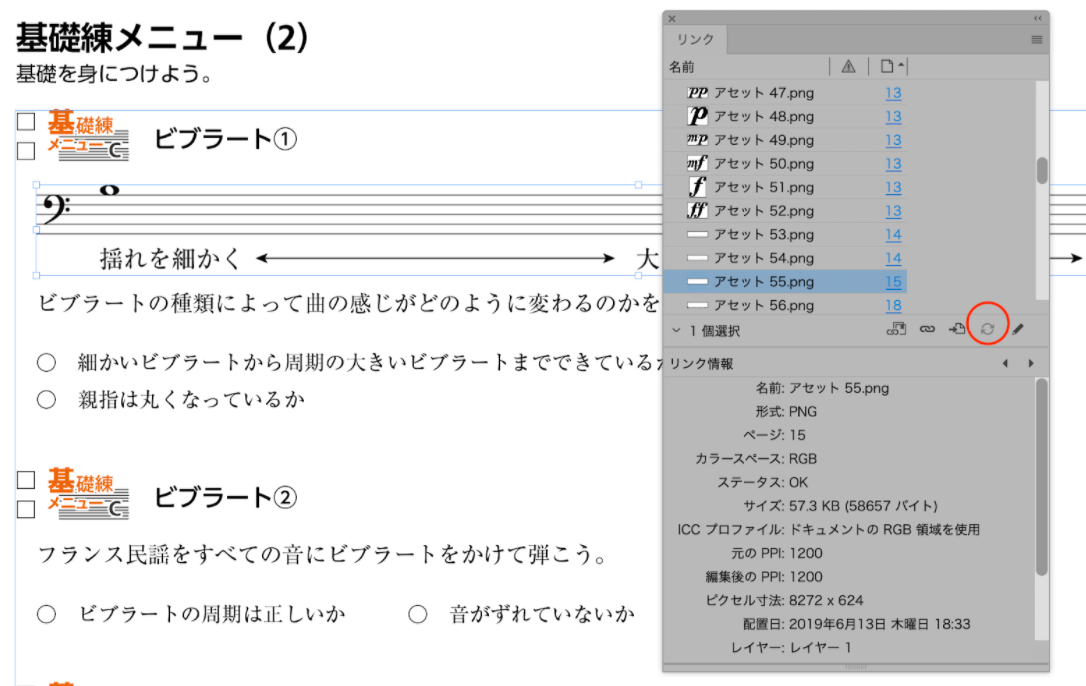
\includegraphics[scale=0.7]{assets/pmh0.png}
\end{figure}

\subsection{入稿、カラーモードについて}
ただし、必ずCMYKで作りましょう(とくにいじらなければOKです)。CMYK,RGB以上にも紙質によって微妙にプレビュー用のカラーセットがあるのですが、そこに関してはたぶんそこまで余裕がないと思うの割愛します。

GoogleDriveFileStreamを使うとファイル管理が楽です。くわしくはかいぬまに教えてもらってください。

ウィンドウ $\rightarrow$ 出力 $\rightarrow$ 分版プレビュー $\rightarrow$ 色分解でcmykで作られているか確認しましょう。黒のチェックを外して黒文字が消えれば基本大丈夫なはずです。


\subsection{入稿時の設定}
ファイル $\rightarrow$ 書き出し で次のような画面が出現します。いじる場所は4箇所です。
(上から順に)
\begin{figure}[H]
  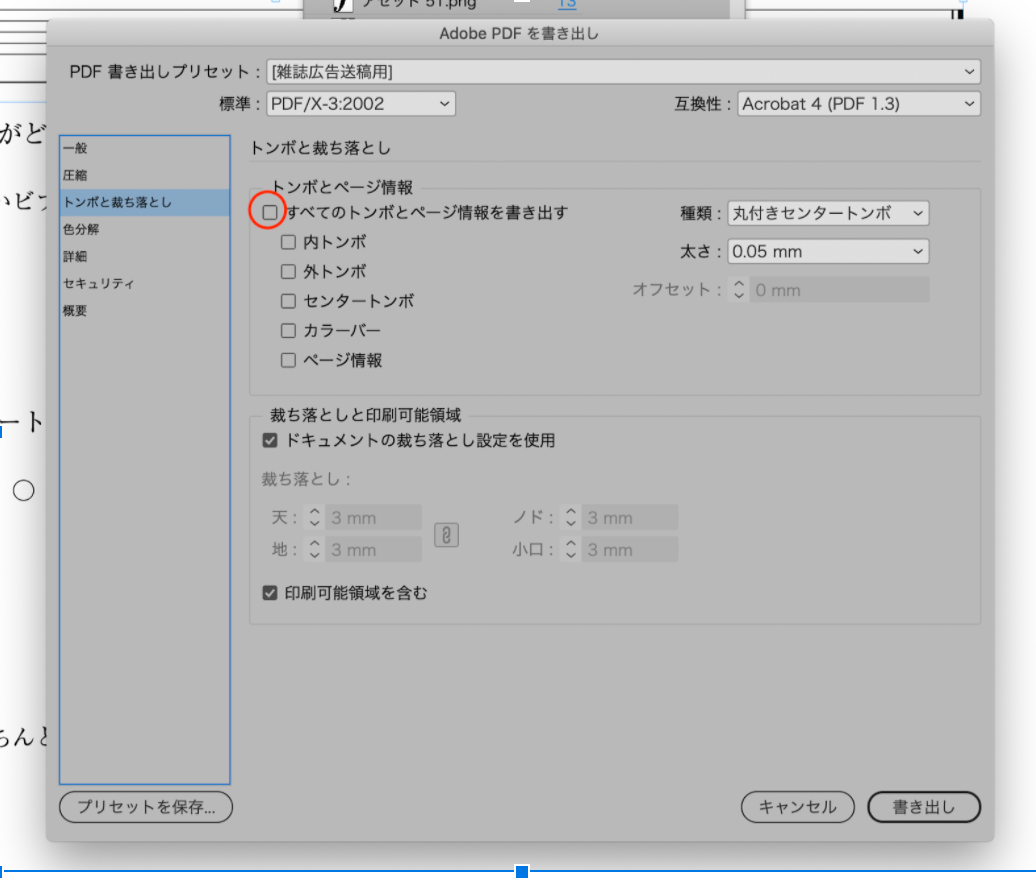
\includegraphics[scale=0.7]{assets/pmh1.png}
\end{figure}
\begin{enumerate}
  \item まずプリセットを雑誌広告送稿用に設定
  \item ページ書き出し範囲
  \item 圧縮(トンボと裁ち落としの上)\\
  校正時などに適当に画像をダウンサンプリングするとよいでしょう。入校時は1GBとか2GBになってもになっても元品質で書き出すことをすすめます。要するにテストで書き出すときのみいじりましょう。
  \item トンボと裁ち落とし\\
  下画像赤丸をクリックします。それで入稿するといいと思います。(ちなみに裁ち落としと言って編集画面を見るとページ外に赤い線がありますが、そこまでデザインをすると良いでしょう。詳しくはかいぬまにきいてください)
  \begin{figure}[H]
    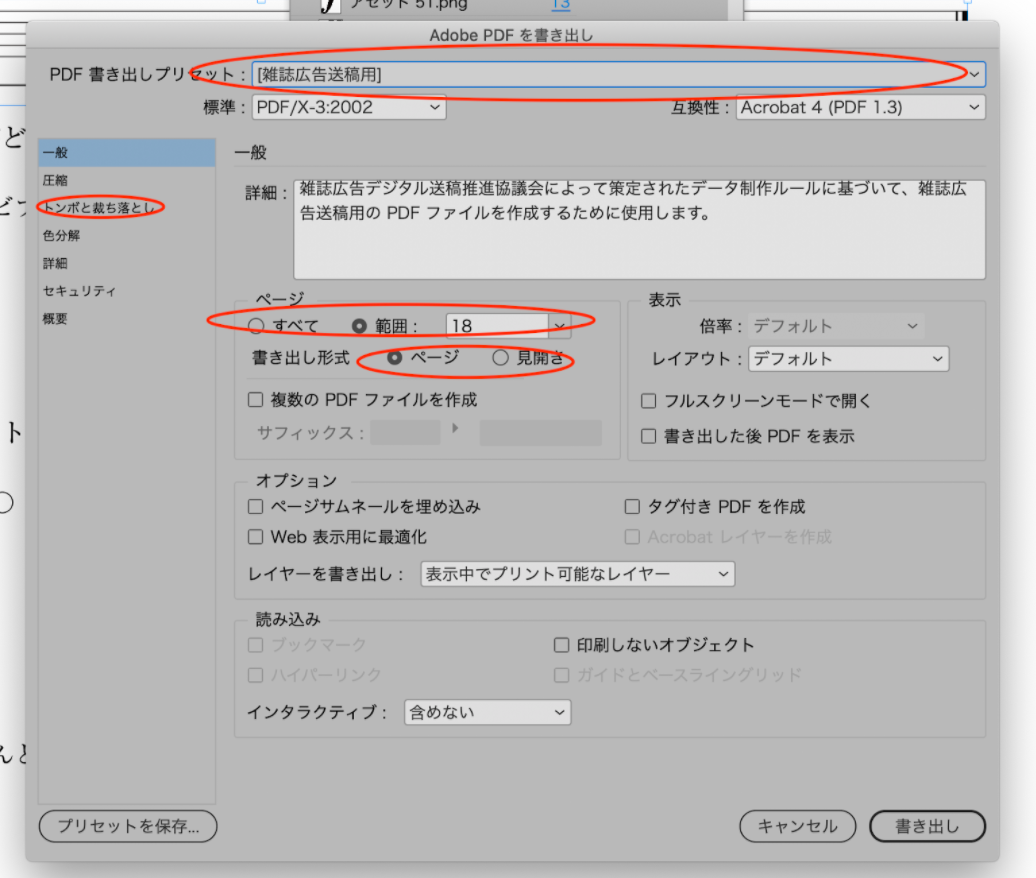
\includegraphics[scale=0.7]{assets/pmh2.png}
  \end{figure}
  \item 以上の作業後 1 でいじったプリセットが雑誌広告走行用(変更)となりますが気にしないでください。
\end{enumerate}

\subsection{フォントについて}
基本的には好きなものを使っていいですが、基本のゴシック体、基本の明朝体を選ぶとらくだと思います。今年はAXISフォントという和文フォントにHelveticaの欧文を合わせて使いました(合成フォント)。くれぐれもMS明朝とかは使わないようにしましょう。美しくないフォントを使うと全体が貧相に見えます。わかりやすい〈使うと良いフォント〉と〈使うのをためらったほうがよいフォント〉の見分け方は、OpenType形式(前者)かTrueType(後者)かです。フォント名の横にTとでてるのがTrueType、OとでているのがOpenTypeです。

\subsection{ページごとの説明}
4月開催ver 資料集めのシート:ページ割り 3/23以降を参照。今年のものは実物を見てください。管轄は上記参照。
\begin{enumerate}
  \item 表紙\\デザイン局に投げる。
  \item 校長実行委員長生徒会長挨拶\\パンフ写真を撮ってくれる専属カメラマンを校内で雇うといいと思います。62回は三枝でした。挨拶文に関しては、校長は実行委員長にいってもらってもらってください(たぶん吉岡さんを経由しているんだと思います)。校長はだいたい提出期限が来ても提出しない(2/2の確率です)ので余裕を持ってお願いしましょう
  \item その他ご案内\\実行委員長とかと相談してください。
  \item 特別企画\\執行部と密に連絡を取り合ってください。
  \item タイムテーブル\\いつまでたっても出来上がりません。頑張って作ってください。僕のタイムテーブルの作り方はかなり特殊だと思います(5分おきの行を数十行作ってそれをセル結合)が参考になったら参考にしてください(ソースファイル参照)
  \item ライブハウス\\全然出てきません。頑張ってください。
  \item Mr.聖光\\今年みたいに一枚の写真撮るといいんじゃない?三枝が企画ととりました。
  \item 地図\\立ち入り禁止区域を明確にしてもらいましょう。また、教室配置は中でやっているものが企画であれなんであれ展示管轄だったはずです(こういうめんどくさいのを一旦全部理解してください。管轄シートを見ればわかる、は、ず)。ただし、紹介文は展示と企画と食品で別々です。
  \item 食品\\食品販売は地図にも後述の食品特集にも紹介文が載る特殊パターンです。こういうよくわからない構造になっているところをどんどん変えていってください。作りやすい方向に、わかりやすい方向に構造を変えるのも立派な仕事です。
  \item 索引\\61回はそもそも掲載方法がジャンル別だったのでさくいんは設けませんでした。地図上での説明の一方でジャンル別の掲載としてさくいんを作るという考え方がいいと思います。\footnote{60回の経験を飼沼が書きます。死ぬほどミスが出て死ぬほど時間がかかります。}
  \item 広告\\サイズが違うと絶対ダメです。外務とちゃんと話して
  \item スタンプラリー\\あるんだったら台紙を載せましょう
  \item 奥付・編集後記
\end{enumerate}
掲載方法についてはここでの説明と9月開催用に実際に作ったもので随分違うのでどちらも参考にして最適なものを作ってください。

\subsection{おわりに}
形はどんどん変えて、わかりやすいものを作ってください。地図とか引き継げるところは引き継ぎ、もっとよくできるところはどんどん改善していく、そういうメリハリが大切だと思います。
僕からは以上です。頑張ってください。なにかあったら何でも聞いてくださいね。\footnote{いや柴田先輩じゃなくて前年の幹部にね}

  \section{HP局}
 62回局長:李
 \subsection{ソフト}
 あくまで僕が使用したソフトである。htmlとcssとjsをいじれるならなんだっていい。
  \begin{itemize}
  \item Visual Studio Code\\
  エディタ。自分好みに機能やデザインをカスタムできるため、汎用性が高い。Microsoft社製でもちろん無料。同じようなものでGitHubが出してるAtomというものもあり、個人的にはAtomの方がデザインはいいと思う。VSCodeにAtomizeというプラグインを入れてAtom風にしていた。プラグインは後ほどまとめる。
  \item Adobe XD\\
  UI/UX設計ソフト。他のAdobeソフトとの互換性がとてもいい配置ソフト。オブジェクトを配置してサイトのUIを検討することができる。直感的に操作でき、画面遷移もシュミレートできる。ただし、CSSやHTMLを書き出してくれるわけではないので必須ではない。個人的には仮でもUIのイメージがあると作りやすいので必ず使っている。
  \item Adobe Dreamweaver\\
  ウェブアプリ制作の統合型開発環境的なもの。初期段階で使うことを検討していた。ウェブ制作のすべてがここにある。リアルタイムのUIシュミレートやサーバーへの更新設定、サイトの公開もやってくれる神ソフトだが、重いのが難点。パソコンを変えたときにインストールを忘れていて自然消滅した。正直全く不満はなかった。
  \item その他Adobeソフト\\
  デザイン局が忙しそうだったので素材は全部自分で作った。楽しい。Illustratorは使えないと恥ずかしい。
  \item FileZilla\\
  いわゆるFTPクライアントソフトというもの。FTPサーバーにファイルをアップロードするときに使う。FFFTPとか有名どころは他にもある。すべてUIが古いWindows感でてて怪しいが全然普通のソフト。FTPについては後ほど解説する。
  \item Firefox Developer Edition\\
  ブラウザ。Chromeでブラウザアカウントを学校アカウントにしてると開発者モードが使えないのでこれを入れた。Developer Editionのとおり、開発者に嬉しい機能が割とある。Chromiumで動いているので環境はあまり変わらないはず。
 \end{itemize}
 \subsection{フレームワーク}
 僕が使用したフレームワーク。
  \begin{itemize}
 \item nuxt.js\\
 サイトが作りやすくなるフレームワーク。流行ってるので使った。必須ではないかな。
 \item firebase\\
 サイトをホスティングするのに使った。詳しくは体験談を読むこと。
 \end{itemize}

 \subsection{スケジュール}
 \begin{itemize}
 \item ベースデザインの確立(1週間)\\
 デザインを設計する上で大切なのは指向となるベースデザインだ。例えばモノクロでいくのか、パステルカラーを使ったハイトーンでいくのか、はたまた原色よりの複雑なデザインにするのか。文面や口で説明するのは非常に難しいがPinterestを使うといい。Pinterestは自分が気に入ったアイディアを保存でき、その傾向によってまたタイムラインを更新してくれるというもので使い方などは各自で調べて欲しい。これを利用することで自分の好きなデザインを集めて考えることができる。スローガンになるべくあったものを探すべきだが自分の場合、これが好きだとおもったデザインに後ほど意味づけを行なった。意味づけとはデザインのオブジェクト一つ一つに意味を持たせることである。この作業は単に意味を頭の中でつけるのではなく、実際にオブジェクトをつけた意味に近いものに修正しながら行う。これをみた1人でもいいからこの意味に気づいて欲しいと思いながらやる。実際はだれもわからないものでもその意味づけの改変がデザインをより良いものとしていく。
 \item オブジェクトの配置(1週間未満)\\
 ベースデザインが決まれば次は実際に作ってみる。紙でもPC上でもホワイトボードや黒板でもいい。一回それを簡単な方法で表現してみる。自分はスケッチブックに一回書いて修正し、ある程度できたら今度はAdobe XDで表現し、また修正するというプロセスを踏んだ。いきなりソースコードを書くと一つのオブジェクトを配置するのに時間がかかる上、修正の小回りが効かない。説明する順番は逆になったがこれが終わったら先述した意味づけを行う。
 \item 環境の構築(1日〜数日)\\
 ローカルにプロジェクトをつくって環境を整える。併せてFirstCommitをしてRemote RepositoryにPushする。
  \item ホームの制作(2週間)\\
  ホーム画面は公開前に終わらせる。他の画面はどうせ素材(画像や紹介文)が揃わないので随時更新でよい。長い時間をかけていいので緻密に作る。載せる内容はトップ\footnote{開いたときに表示されるやつ}、お知らせ\footnote{告知のなかから抜粋}、スローガン\footnote{スローガン動画公開まで非表示}、実行委員長から\footnote{ポエム}、フッター、サイトマップやメニュー。他は自由に追加して構わない。
  \item サイトの公開\\
  聖光祭開催1ヶ月前を目安に公開する。その後、SNSや学校のサイトで宣伝する。個人的には1ヶ月前だと遅い気すらする。
  公開には時間がかかるため、SNSや学校のサイトで告知される前にはもう公開しちゃおう。(どうせ調べても出てこない)その際、しっかりSEO対策\footnote{SEO対策とはGoogleなどの検索エンジンロボットにサイトの内容をより正確に取得してもらうようにすることを指す。}をする。僕はサボっててサイトの説明文すら書いてなかったが途中で気づいて書いた。サイトの公開後はGoogleSearchConsoleにサイトを登録。Google検索で自分のサイトがどれくらい検索されてて掲載順位がどのくらいなのかをみることができる。GoogleRobotがどのくらい来たかもみれる。登録にはサイトの所有者を証明する必要があるため、Googleからもらったhtmlを直下に置いたり、metaタグを追加したりする。所有者が証明できたらとりあえず安心できると思う。3日後ぐらいまでには記録が開始され、掲載順位や訪問者数のグラフが表示されるだろう。
  \item サイトの運営\\
  聖光生や暇な先生って結構優秀で間違いやバグを報告してくる。その報告を修正しながら、次のサイトの制作を始める。
  \item サイトの順次更新\\
  情報がUpdateされるごとにサイトを更新していく。展示団体が確定すれば展示団体一覧を、食品店舗が確定すれば一覧を、校内Mapやスローガン、余裕あれば取材などして記事を投稿するのもいいだろう。ある程度自由にできるので楽しもう。
 \end{itemize}
 \subsection{ウェブサイトを作る上での基本知識}
 余計なお世話かもしれないが、最低でも以下のことは覚えとこう。
 \subsubsection{リクエストとレスポンス}
 端末からサーバーへの問い合わせ(Request)とそれに対する応答(Response)の関係は何があっても覆すことはできない。Requestなしにサーバーがいきなり端末に通信をすることはできないのである。
 \subsubsection{サーバーという概念とURL}
 我々が使うのはおもにファイルサーバーというものである。他にアプリサーバーやDBサーバーが存在する。URLはサーバーに存在する全てのアクセス可能なファイルに対して与えられ、パスと同義である。URLのオーソリティはサーバーを特定しその後は設定したルートファイルからの相対パスになっている。オーソリティはプロトコル、サーバー名、ドメインでできている。例えばPC名www、ドメインseiko.ac.jp内のroot/2021/articles.htmlのファイルのURLはhttps://www.seiko.ac.jp/2021/articleとなる。プロトコルとドメインは次項で解説する。
\subsubsection{プロトコル}
プロトコルとはある通信が何についてのどんな形の通信なのかを表す規定された文字列のことである。当然この世界にはWebサイト以外の通信もあり、物理層、データリンク層、ネットワーク層、トランスポート層、セッション層、プレゼンテーション層、アプリケーション層の7層でできている。下の層になるほど物理的で単調な信号になる。これはあくまでプロトコルの分類の概念である。ちなみにこの概念はOSI参照モデルといって現在はTCP/IPという別の概念が使われている。端的に言えば「何を送るのか」を表しているのである。例えばHTTPはウェブサイト、HTTPSは暗号化されたウェブサイト、SMTPはメールの送信、POPやIMAPはメール受信\footnote{厳密には移動とコピーの違いあり}、FTPはファイルやフォルダーの送信などがある。アクセスしたファイルをどんな形で取ってくるのかを表し、ブラウザがレンダリングするときに使われる。
\subsubsection{ドメインとサイト取得までの流れ}
今回は作りたての学校のHP http://www.seiko.ac.jp/ に自宅にあるPCから始めてアクセスした時を考えてみる。\footnote{なんでhttpなんだよ...} まず、URLを叩く。その通信は無線LANで繋がっているルーターから自宅地下の電話線を通り近くのキャリア基地局までくる。データセンタとも呼ばれるところである。\footnote{Googleデータセンタなどのデータセンタとは別物}URLはネットの住所ではないのでURLだけで直接どこかにアクセスことはできない。使用するのはIPアドレスであり、とりあえず聖光HPのIPアドレスを探したい。ここで一度基地局内のキャッシュサーバを通しキャッシュから探す。今回はサイトも端末も新しいので以降のすべてのキャッシュサーバでキャッシュに何も保存されていないこととする。キャッシュサーバ通したときに履歴が残っていればそこで必要な情報が折り返されると考えて良い。

キャッシュになかったため、権威DNSサーバにアクセスする。ドメインは逆側から読む\footnote{今気づいたけど外国の住所と同じやな}のでjp\textgreater\textbar ac\textgreater\textbar seikoという構造である。権威DNSはjpノードに案内し、jpノードはsc(教育機関)ノードに案内する。そしてscノードにはseikoという名前のサーバのIPが登録してありこれを取得する。これでURLとIPの交換が完了した。通常はどっかのキャッシュに履歴が残ってるのでscノードには普通行かない。ドメインは入れ子構造になっていて逆から読むということは覚えとくべき。

もらったIPを使えば簡単に聖光のルータにアクセスできる。ルータからPC名(今回はwww)を渡すことでパソコン内のルートフォルダにアクセスする。パスには今回何も書かれてないが/で終わることは暗示的にindex.htmlを指すことが設定されてるはず\footnote{場合によってdefault.htmlなど、サーバ側の設定で変えることはできる}なのでindex.htmlを取得し端末に帰っていく。
\subsubsection{サイトのレンダリング}
HTTP通信のうち、サイトのhtmlを取得したりする\footnote{一般化するとdoGet()をコールするということだが}ことをGET通信と呼ぶ。これに対して、サーバに対して情報を渡すときに使うのがPOST通信である。先述したindex.htmlをGETするのが第1ステップになっており、そのhtmlを取得したブラウザは\verb|<head>|タグを読む。そこには\verb|<link>|タグや \verb|<script>|タグでcssやjsが紐づけられており、今度はこのcssやjsをGETしにいく。その間に\verb|<body>|タグ内を読み、\verb|<img>|タグや\verb|<video>|タグ、\verb|<iframe>|タグなどのリソースを取りに行く。また、読み込んだ\verb|<body>| タグ内のオブジェクトを描画し、cssをもとに再描画。\footnote{この間僅かなので見えない。ネットが遅いと見れる。}最後に\verb|<img>|タグや\verb|<video>|タグ、\verb|<iframe>|タグなどのリソースが届き、当てはめる。javascriptが実行され、すべての作業は終了する。以上を見るに何回もGETを繰り返してるのがわかる。これは開発者モードで見ることができる。
\subsubsection{FTPクライアントの使い方}
FTPサーバにファイルを送信したり取得するときは「FTPユーザ名」と「FTPパスワード」と「FTPホスト」が必要である。「FTPユーザ名」はドメインと同じなのでseikofes.official.jp。また、FTPホストはsv64.star.ne.jp。この三つは一緒にITEC長のパスワード一覧的なものに掲載してもらってる(はず)なので、部門長に問い合わせてみること。FTPクライアントに少し名称は違うかもしれないが、この三つを入力する。あとは接続ボタンを押せばOK。僕が使ったFileZillaは左側にローカルのファイルツリー、右側はFTPサーバのファイルツリーが表示されており、ドラッグ\&ドロップでファイルを移動できるようになっていた。また、Starserverの方からもアクセスでき、ファイルのアップロードはできないが確認としては役立つだろう。
 \subsection{反省点\&注意事項}
 \subsubsection{顧問挨拶}
 部門の顧問の生成と挨拶するときにかならず「starserverの代金は払っているかの確認」をしてもらうようにすること。今年2021年、3人の先生に確認して「払っている」と言われていたが結局、支払い催促メールが届いていた seikofesta@gmail.com を誰も見ておらず、契約解除となってしまった。(もともとは seikofesta.official.jp だったと記憶している)seikofesta@gmail.com にアクセスできる唯一の先生が夏季休暇のため音信不通になってしまったのも起因してしまった。夏休み中は先生と連絡できるとは限らないのでもし、聖光祭の開催時期が2学期だった場合、注意が必要である。
 \subsubsection{時間を作ろう}
 基本的にHPの仕事がメインだと思うが自分の場合はそうではなかった。むしろ副業みたいなものだったので時間はあまり作れなかった。これによってHPは中途半端なところで終わってしまった。食品店舗は終了したのでCOMING SOONを表示してると思うが、マップや記事ページは終わってない。記事は投稿できる仕組みを作ったが、Firebase Realtime Databaseにデータ入力する必要があり時間がなくてほとんど投稿できなかった。これは猛省している。麻布(2020?)ではアカウント制にしており、幹部などが自由に書き込みできる。(自分の代はそうゆうのを逆手にとっていたずらする問題児がいたのでどちらにしろ実現できなかったが)その代の風紀を鑑みた上、人を絞るあるいは記事投稿班を作るなどしてやってみるのも面白いと思う。灘(2019)ではMarkdown記法をHTMLに変換するライブラリを使っていた。いちいちサイトを更新しなければいけないがいい考えである。\footnote{2019灘の文化祭「SAIL AWAY」のHPは高校生が作ったと思えない神サイトである。ぜひ一度見て欲しい。}
 \subsubsection{仕事を整理しよう}
 HP制作中は素材関連の連絡や修正の申し出、仕様変更の申し出などが多くあり、HPに掲載する情報を整理するだけで一苦労である。付箋を使ったタスクの管理は古いと思われがちだが、あれはすごい効果的だ。自分は自分の席が壁列だったので壁に付箋を貼っていた。それによって仕事が捗ったのは事実だ。PC上で管理できるが結局は開くのがめんどくさい、タスクの登録がめんどくさいなどで逆効果だった。ぜひ取り入れて欲しい。
 \subsection{Tips(コーディング上の注意・小技)}
 \subsubsection{positionは使うな}
 positionはcssでオブジェクトの対外関係を設定できるパラメータである。が、これは書くな。領域が表示されないときに適当にいじってると階層関係がぐっちゃぐっちゃになる。また、position: absolute;を設定しないとできない、領域を重ねる必要があるUIをデザインしないこと。


 \subsubsection{JavascriptでUIを構成するな}
 Javascriptを使うことによって画面の大きさを取得し、それを踏まえて数値を設定できるのは確かだ。しかし、cssの適応からjsが動き出すまでかなりタイムラグがあるのでユーザー視点では画面の表示後、少しカクツクように見える。また、ぱっと見なのをしているか−−−具体的には何をどこに配置してるかがわかりずらい。じゃあどうすればいいのか。答えは簡単でjsを使わなければいけないほど複雑なUIを実装するのは−−−またはUIを実装するのにjsを使わないといけないほどのスキルしかないのであればこの仕事はあなたには無理だ。ということだ。もちろんスクロール位置を変えたり、classをトリガーで付与したり、時間差で剥奪するのはjsでしかできない上、視覚的に何をしているのかわかるのでそこでjsを使ってもらって構わない。

\subsubsection{idをcssで使うな}
これ読んでる人の中ではidは固有、classは種類と習った人が多いと思う。しかし、−−−これはあくまで僕の意見なのだが−−−idはjsに使い、classはcssに使うというふうに設定したほうがいいと思う。現に多くの企業のコーディング要項をみるとそのようになっている。しかし、jsで複数の要素に対して操作を行いたいという場合は結構ある。なのでjsでcssを使わざるを得ないのだ。ただ、idをcssを使うのはやめること。cssは基本、classのみで作る。

\subsubsection{命名規則を守れ}
ウェブサイトの制作はそこまでスキルを求められない。むしろ情報量との戦いである。というより、莫大な情報を脳内で整理、あるいはコードで整理するそのことが"スキル"と言える。画像や文章などの素材、デザインや色などの要素、cssとjsとhtmlを反復横跳びするたびに忘れていく"目的"。コーディング中は求められるコーディングスキルとは相反してかなりのストレスがかかるだろう。そんななか、名前を見ただけで内容を理解するために命名規則を守ること。命名規則を守らないならこの仕事をする価値はない。詳しくは{\bf\ref{sec:命名規則}}を参照。

 \section{アプリ局}
 \subsection{Android}
 \subsubsection{はじめに}
 引継書とは題しているがAndroid作る人は全員読んでおいて損はないのではないかと思われる(今年出してもらったプログラムの出来栄えを見る限り)。\par
かなりメモっぽく書いているので注意。Discordで皆に連絡
するときの感覚で書いていると思ってもらえると内容が入りやすいかもしれない。
 \subsubsection{技術幹部になった人へ}
 個人的に技術幹部となった人に要求されることは高い技術力よりも仕事をミス無く丁寧に確実にこなすことなので注意(もちろん自分の担当する分野においてある程度の知識は持っていなければいけないけれど)。技術力があったとしても、
 \begin{itemize}
 \item 提出期限を守らない
 \item ミスが多い
 \item 連絡ができない
 \end{itemize}
 といった人は技術幹部に限った話ではないけれどお仕事にならなかったり、もしくは周りに迷惑を書けてしまい他の幹部に陰口を叩かれてしまったりする(後者はよく見た気がする)。\par
くれぐれも技術力があるからといって他の部門の幹部などに対して調子に乗った言動をしたり高圧的になったりすることがないように(まぁこんなことはほぼなかったと思うけど)。
 \subsubsection{全体として}
  \subsubsubsection{制作の前準備}
 今回なら聖光祭は9月で、UIなどの案が挙がってくるのが8月であったけれど、アプリの試作自体は5月から始めていた。\par
 特に自分に作ることができるか不安な箇所を中心に自分で事前に試作をしておくとよい。
 矢向なら
 \begin{itemize}
  \item RecyclerViewの使い方
  \item RecyclerViewを横に2つ、それを縦につなげていく方法
  \item HTTP通信
  \item Fragmentを画面に一部に収める(全画面に出さない)
  \item DBの使い方
  \item アプリアイコンの設定法
 \end{itemize}
 など
 \subsubsubsection{実装方法の基本方針}
 同じ挙動にもいくつかの実装方法が当然考えられるわけだが、どの方法を使うかを選ぶときに重要なことを重要度順にあげていく。
 \begin{enumerate}[No.1]
  \item エラーが起こりづらいこと(起こらないこと)
  \item 動作が軽いこと(=ユーザーが快適に使えること
  \item コードが読みやすいこと(=保守性が高いこと)
  \item 実装方法がオシャレであること
 \end{enumerate}
1と2は最優先事項。とくに1。カッコつけて新しいライブラリを使ってエラーが起こりました、ではお話にならない。また、この4点はお互いに関係があり、1つを守ることが他の2つを守ることにつながっていくので常に頭に入れておきたい。
 \begin{itembox}[l]{余談}
 現在唯一人間を国際宇宙ステーションへ輸送することができるロシアの有人宇宙飛行船「ソユーズ」では、動作環境が宇宙空間であるために事故は絶対に起こってはならず、そのためソユーズを制御するコンピューターにはあえて新しいものではなく、動作が保証されたかなり旧式のものが使われてるそう(ソユーズに限った話ではないけれど)。つまるところアプリ開発においても古いライブラリなどを使えとは言わないけれど(というかむしろ古すぎると逆にエラーが起きることが多い)プログラムの安定性を最優先にしましょうということ。\par
 \begin{center}
 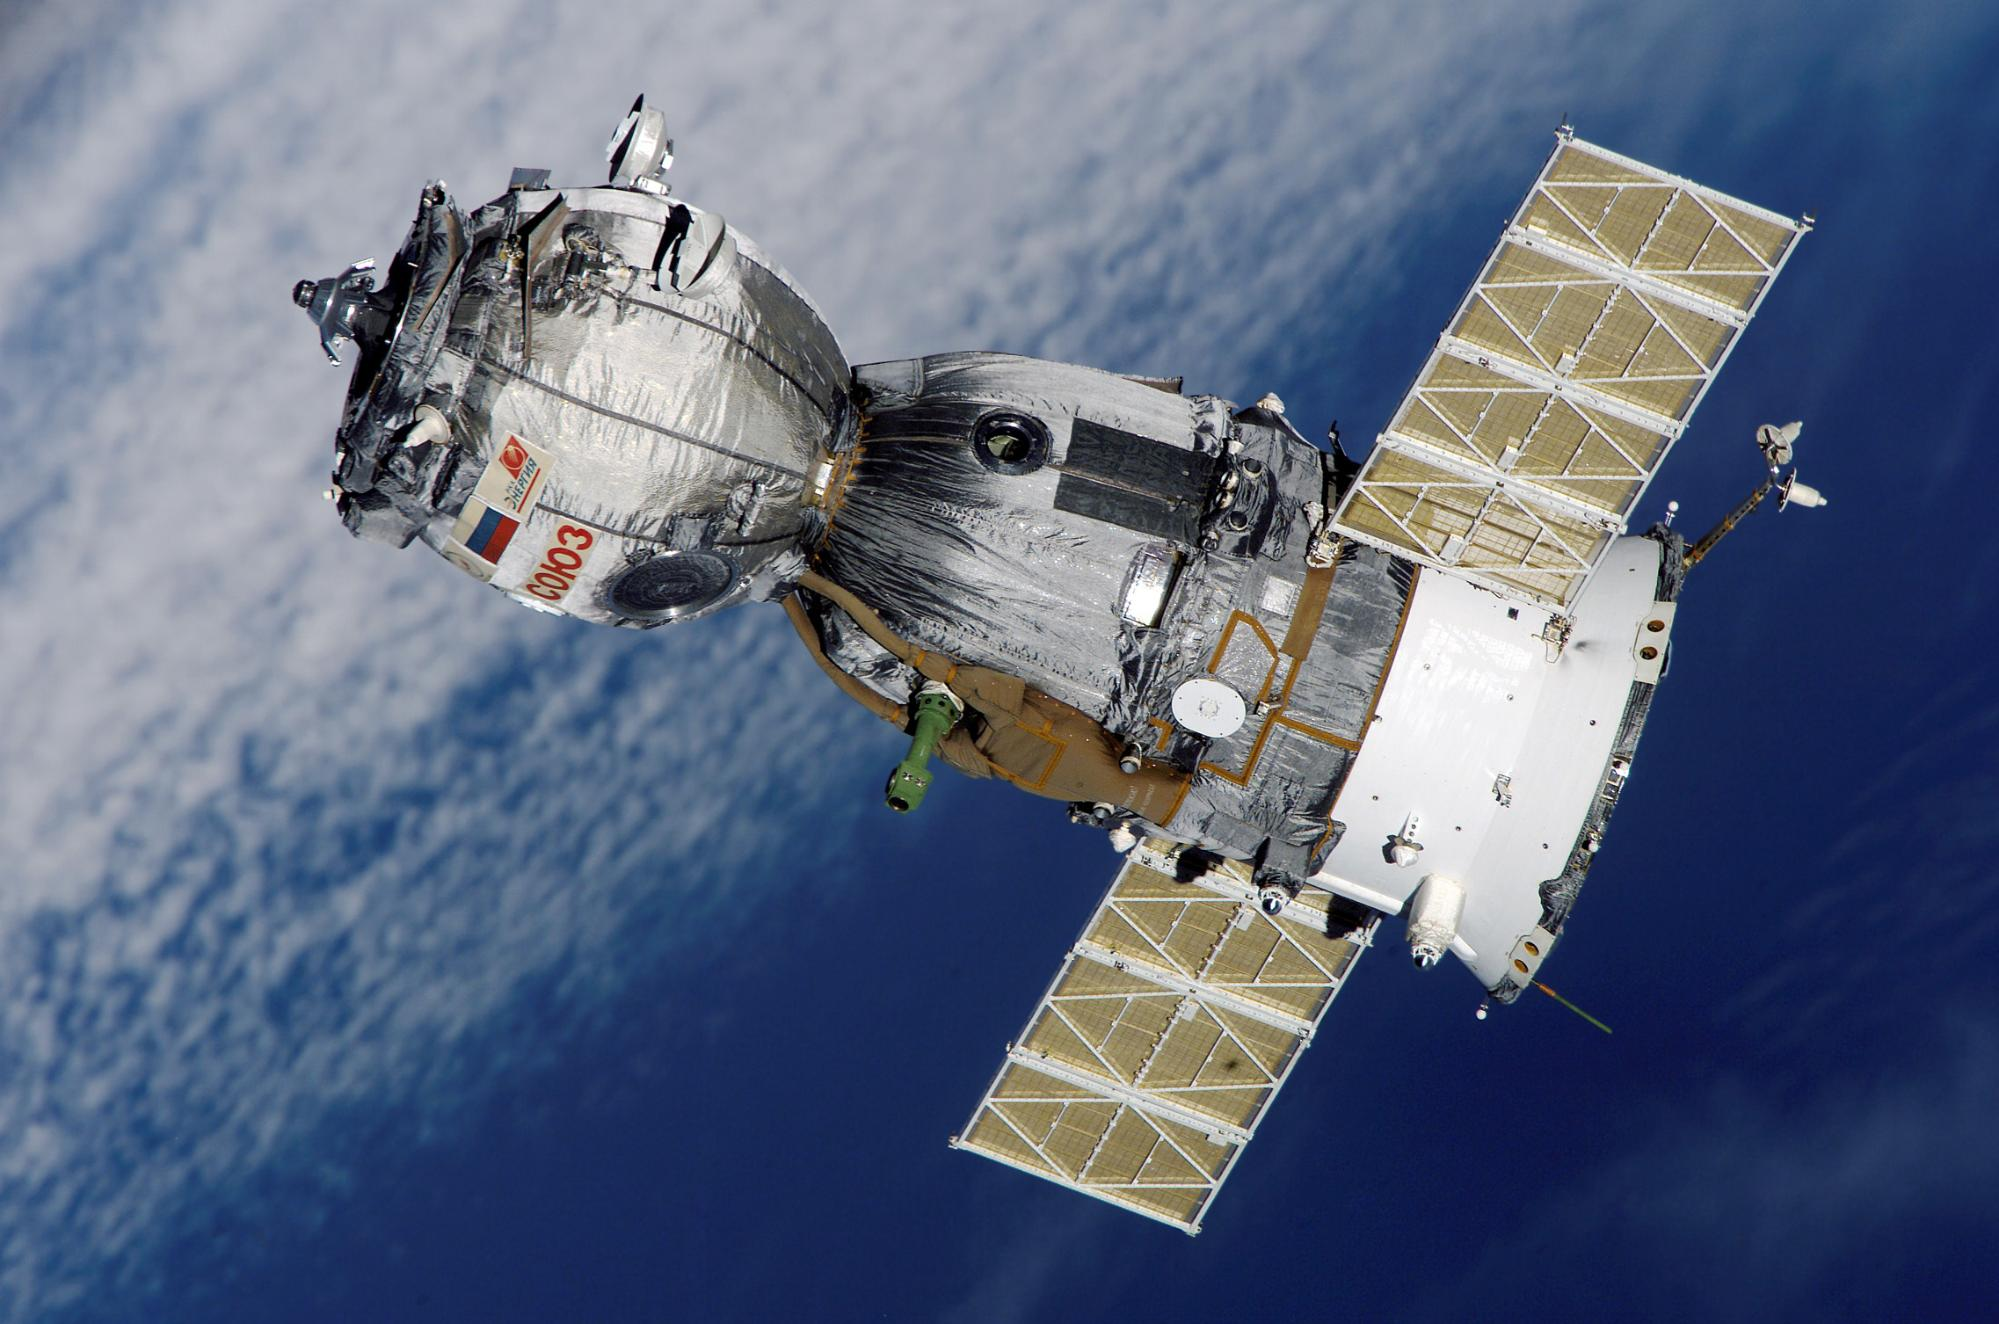
\includegraphics[scale = 0.1]{assets/soyuz.jpg}
 \end{center}
 \end{itembox}
  \subsubsection{素材について}
 基本的にデザイン局の方と連携を取りながら行っていく。\par
今回の場合はこちらが最初にデザイン案を作りそれをデザイン局の飼沼とブラッシュアップした。\par
 \subsubsection{各画面について}
 全体として今回矢向は李のアドバイスを勘違いしMainActivity以外全部Fragmentというあまり類を見ない設計にしてしまったので参考になならない箇所もあると思われる。
 \subsubsubsection{ツールバー}
 \begin{minipage}[b]{13.5cm}
 Androidの機能も用いて作ることもできる。\par
 だがしかしこれだと取り回しがあまりにも悪いので、右図のようにactivity\_main.xmlにて画面をLinearLayoutで分割し、上(赤い部分)にはツールバー、下(青い部分)をRelativeLayoutにしてFragmentContainerにし、ここだけでフラグメントを置き換えるようにするとフレキシブルなツールバーを作成できる。詳細は以下のリンクから。\par
  \url{https://qiita.com/mi_iroha/items/c8b6a1a6262c77e28301}\par
  この時普通のツールバーのメニューはどのように出すのかという疑問が出るかもしれない。結論としてはDialogFragmentを継承したダイアログを位置を右上などに指定して出す(指定方法は調べればすぐに分かるので割愛)。
 \end{minipage}
 \begin{minipage}[t]{3cm}
 
\includegraphics[width=3cm]{assets/ToolBar.png}
 \end{minipage}\par\par
ツールバーのonClickの実装を各Fragmentでしなおすことで(今回は各FragmentのinitToolBar()やonCreateViewにてその処理を行っている)各画面で違ったクリック処理を行うことができ、またその際に現在のFragmentのメンバ変数などにアクセスすることもできるようになる(匿名クラスを使えばより楽にonCreateView()内の変数にアクセスできる)。
今回はActivityがひとつなのでこれだけで無事に作成することができたがActivityが複数ある場合はもう少し工夫が必要だと思われる。
 \subsubsubsection{ホーム画面}
 ImageViewおいてclickのListenerつけるのみ。難易度はかなり低い。
 \subsubsubsection{展示一覧}
 RecyclerViewを配置するだけではあるが、絞り込み機能があるため少し難易度が高い。\par
 全展示団体のデータをDB(と今回は混雑度のサーバー)から取得し表示する。\par
 その際にRecyclerViewのAdapterに渡すListを作るとき、絞り込み条件に合致しないものはforループの最初にcontinue文で弾けばよい。
 \subsubsubsection{食品一覧}
 RecyclerViewを配置するだけ。メモ帳が理解できていればかなり難易度は低い。

 \subsubsubsection{マップ}
 まず地図の画像はパンフが出来上がったらその画像を使うとよい。出来上がるまでは途中経過の地図を使ってプログラムを書いてく。地図の画像、展示団体等の位置を識別するための画像、ピンの画像、タブレイアウトをおくためのFragment、タブレイアウト内に表示するためのFragment、タブレイアウトの機能を実装するためのAdapterはおそらく必要となる。加えて、地図の操作を行うためのカスタムビュー等も用意することになるだろう。\par
 次に、各機能の詳細について書いていく。\par
 タブで階数ごとに違うマップを出すようにする。タブレイアウトはここをみればわかると思うので詳細は省略する。\par
マップのドラッグ、ズームについては画像をMatrixを使用して移動、拡大縮小するのがよい(画像の座標や、拡大率とかを保存しておくと後々楽になり、Matrixならそれらを保存してくれるから)。描画方法はimageViewを用いる方法とcanvasを使用する新しくViewを作って用いる方法などがあるが今年はimageViewを使用した。どちらもMatrixを使用して移動等が可能。ドラッグやズーム等の検知はGestureDetectorを使って検出した。ドラッグはonScroll、ズームはonScaleで係数を取得することが可能。地図の端に到達した判定は、どこを端と定義するかによるが、今年は「画像の端がスクリーンの真ん中を超える」という判定とした。地図の端をどう定義するかは、色々な外部のサービスを参考にすると良い。慣性は余裕があるならば実装するのが良いが、少し厄介であるため無理して実装しなくてもよい。今年は慣性をonFlingで取得しTimerで動かした。また、画像の端を超えたあとや、ズームで縮小しすぎたあとに戻す処理でもTimerを使用し、滑らかな動きを実装した。\par
マップの操作云々を調べて自分なりの実装が難しいと感じたら\link{李のQiita}{https://qiita.com/Cyber_Hacnosuke/items/b2a8724218d2f4a4c3c2}を参考にしてください。\par
「タップした場所がどこなのか」を判別する方法は、別途、各展示、食品で色分けされた画像を元に判別する。タップしたスクリーンの座標から、画像の位置座標と拡大率を用いてタップした画像の中の座標を算出し、色分けされた画像のその座標が何色かで判別する。今年は、\verb+ #FF00XX(XX / 2 = id) +が展示、\verb+ #00FFXX(XX / 5 = id) +が食品と決め、色識別用画像を作成した。画像を作るのは自分でやったが、信頼できるなら後輩に頼むと仕事が減る。色識別用画像を作る際、拡大縮小等でボケて、想定していなかった色が検出されないよう気をつけること。\par
詳細画面のピンの座標はデータベースに0~1の範囲で、x,y座標それぞれの割合を記録しておき、表示する際その値から画像用の座標を計算しピンを指してる。この0~1の範囲の座標を計算するにあたり、スプレッドシートを使って計算するのがもっとも効率的と思われる。参考程度に今年使った\link{自分用スプシ}{https://bit.ly/3cm73ig}を置いておく。\par
最後に、地図を表示するには、大きな地図の画像を用意する必要があるが、その際に重すぎて落ちないよう気をつけること。\par
 \subsubsubsection{タイムテーブル}
 1イベントあたりのレイアウトを別途xmlで記述しておく。\par
また、今回の場合は9:00の線と10:00のy座標から1時間あたりの座標変化数を取得しておく
DBから表示すべき全イベントを取得し、それぞれのイベントごとにfor文を用いて先程のxmlファイルをLayoutInflatorでインフレートし、各イベントの開始/終了時間と先程の値を用いてそのViewのTop,Bottom,heightを計算し表示(ViewGroup.addView(View)みたいなのでできる)するとよい。\par
Viewの生成はここを参照することを推奨する。
 \subsubsubsection{トレジャーハント}
 ここに関してはおそらく設計者が次回も(そもそも次回もトレハンをやるのかという問題があるが)ITECの人間ではないので少々我々プログラマサイドからではわかりにくいかもしれない。\par
 いかに内容を噛み砕いて実装できるかが成功のカギとなる。\par
 実装自体の難易度はあまり高くない。
 \subsubsubsection{聖光ラジオ}
 HTTP通信で取得した内容をRecyclerViewで表示するのみ。\par
 応募に関しても、応募する内容をHTTP通信で送るのみのシンプルな処理。
\subsubsection{各技術指導}
 \subsubsubsection{HTTP通信}
 難易度はかなり高い。\par
 この引継書もこれを書くために書いたと言っても過言ではない。\par
 OkHttp3という外部ライブラリを使用した。\par
 implementation group: 'com.squareup.okhttp3', name: 'okhttp', version: '3.14.9'\par
 Gradle(build.gradle(app))に上記の内容を書いておく。\par
 プライバシーポリシーにもokHttp3使用の旨を書かなくてはいけない。\par
 Android(というかGoogle)は画面の描画が遅れフリーズなどをしているようにユーザーに感じられてしまうのを防ぐため、通信処理をメインスレッドで行うとNetworkOnMainThreadExceptionという例外を投げるようになっている。\par
 つまり通信処理はマルチスレッドで行わざるを得ない(こう書いてはいるが通信は別スレッドで行うのがセオリーなのでこれはおかしいことではない)。\par
 JavaやKotlinでマルチスレッド処理を行うには、Threadクラス等を継承もしくはRunableインターフェースを実装したclassのrun()メソッドをオーバーライドし、その中にマルチスレッドで行いたい処理(今回なら通信処理)を書くことになる。\par
 とはいっても今回出してもらったプログラムを見る限り半年でこれを自力で行えるレベルに到達するのは(勉強などを考えると)かなり厳しいと思われるのでFragmentと連携して通信内容を表示する雛形を載せておく{\ttfamily \url{https://qiita.com/Jellyfish4594/private/9709ad41d0828f917601}}。
 \subsubsubsection{RecyclerView}
 \begin{enumerate}
 \item list\_item.xml
 \item RecyclerViewHolder
 \item (保持する値が複雑な場合は)RecyclerStructure
 \item RecyclerAdapter
 \item 表示する
 \end{enumerate}
 の順に作れば5~10分で作り終えることができる。\par
 \link{ここ}{https://qiita.com/Todate/items/297bc3e4d0f3d2477ed3}の内容をほぼコピペで使用することができるが、Adapterのoverrideメソッドの引数に一部が本来はあっていはいけない?がついているため、そこだけエラーが出る(もとのメソッドの引数がnull許容型ではないからエラーとなる)。
 \subsubsubsection{QRコード}
 そこそこに難易度が高い。\par
 \link{これ}{https://github.com/SeikoStudentCouncil/SeikoFestaAndroidApp62nd/blob/master/app/src/main/java/jp/ac/seiko/itec/seikofestaapp62nd/fragments/treasurehunt/QRCodeFragment.kt}をコピペするだけで大部分を完成させることができるが、下記のようにGradleに書かなければならないので注意(ZXingを入れる、OkHttp3と同様にプライバシーポリシーにも書く)。\par
 implementation 'com.journeyapps:zxing-android-embedded:3.6.0'
 \subsubsubsection{Fragmentを一部に表示}
 RelativeLayoutを配置しそれをFragmentContainerにすることでできる。
 \subsubsubsection{GoogleMapを置く}
 \link{ここ}{https://developers.google.com/maps/documentation/android-sdk/start?hl=ja}に従う。
 \subsubsubsection{GitHubでの注意点}
 リリーズビルドしたアプリの実行ファイル(.apkまたは.aab)は画像リソースのサイズによっては100MBを超えることがあり、そうなってしまうとリモートレポジトリにPushできなり、復旧が大変なので.gitingnoreに記載しておくこと。詳しくは\ref{sec:GitHub}を参照。
\subsubsection{リリースについて}
\begin{itembox}[l]{Google開発者用アカウント}
\color{red}
mail: seikosougiken@gmail.com\\
\end{itembox}
これがないとリリースができず詰みとなってしまうので気をつける。
\subsubsubsection{審査について}
李のとき(第60回)は2\UTF{FF5E}3時間で終わったと聞いて油断していたが今回は現在審査に出して72時間ほど経つがいまだ終わっていない。2019年の9月あたりから審査が厳正化しているそうなので気をつけるように。今回もそうだが素材がなかなか来ないのでASAPを心がけるだけでよい。ちなみに審査はおそらくカルフォルニアで行われている。
\subsubsubsection{審査時間の目安}
初回審査...72時間程度=3営業日(遅い場合は問い合わせも手)
それ以降のアプデ...1営業日(カリフォルニアの)
\subsubsection{後輩の育成について}
正直なところ、聞かれたらいくらでも教えてあげることはできるが\textbf{\gtfamily 体系的に教えてあげることができるのはせいぜい} 基本制御構文\footnote{if文やfor文などのこと}や変数などの
\textbf{\gtfamily 全プログラミング言語に普遍的に存在する概念くらい}で、オブジェクト指向やアプリの本格的な作り方などの習得度合いは\textbf{\gtfamily 学ぶ本人の主体性}に依るところが多いと思われる\footnote{おそらくプログラミング系統だけではなくて動画やモデリングなどでもそう}。
ここだけの話「もう来年以降の技術は知らん()」といった会話もよくあった。この手の技術の習得には自分で練習することが必要不可欠だし、ここあたりは勉強に通ずるところもある。よって教える側ができることは
 \begin{itemize}
 \item 質問には必ず答えてあげること
 \item 自分が学ぶときにしてほしかったことをしてあげること
 \end{itemize}
の2点だと思う。
逆に真面目にやりさえすればプログラミングスキルなんて\par
文法+ライブラリの使用方法の知識\par
にほかならないので習得は(オブジェクト指向などの一部の関門を除き)習得は容易だと思う。\par
技術的な習得レベルの目安としては、最低限メモアプリを自力で作ることができなければアプリを「ちゃんと」任せるのは厳しいかもしれない、といった感じ。
 \subsubsection{おまけ1:小技(よくあるちょっとしたエラー)}
 \subsubsubsection{NullPointerException :\UTF{FF5E}Attempt to\UTF{FF5E}という例外が発生する}
 多くの場合findViewByIDをする際の引数のidが間違っている(findViewByIdしているviewの中に存在しないviewを探そうとしているためnullが返されてしまう)。\par
xmlやktをコピペした際にidを変え忘れたり、xmlの場合はDesignタブでコピペしたidを意図したものに直そうとするとAndroidStudioがリファクタリングと勘違いしコピペ元とコピペ先両方のファイルのidを変えたりすることで起こる。findViewByIdは該当するviewが見つからないとnullを返す(らしい)ので代入先がnullableでなかったりする場合に起こる。
 \subsubsubsection{宣言部参照}
 メソッド名や変数名をctrlを押しながらクリックすることでその宣言部にジャンプすることができる。\par
自分が書いたコードでなくても(例えば\texttt{android.view.View}クラスなどでも)可能。
・使用箇所確認
メソッドやクラス、変数の宣言部にてその名前をctrlを押しながらクリックするとそれが今開いているプロジェクトのどのファイルの何行目でどのような引数で使用しているかを一覧として表示することができる。

\subsubsubsection{Database Inspector}
アプリ実行中(DBを使用すれば)下のバーの「App Inspection」からDBの中身をExcel形式で見たり編集したりできる。また任意のSQL文を実行することもできる。デバッグに便利。\par
実行している端末のAPIレベルが低すぎると使えない(確か26以上)。
\subsubsubsection{Layout Manager}
右下の縦のバーにある。アプリ実行中に使うと現在開いている画面がどのViewで構成されているかが分かる。面白いけれど個人的には役に立ったことがない。実行している端末のAPIレベルが低すぎると使えない(確か26以上)。
\subsubsubsection{Profiler}
下のバーにある。実行中に現在どれぐらいメモリやCPUのリソースを消費しているかが分かる。
\subsubsubsection{OutOfMemory}
DBの場合ちゃんとcursor.moveToNext()しているかを確認する。\par
画像を扱っている場合dpi別に画像をリサイズしてdrawable-hdpiやdrawable-mdpiなどに分けて入れておくとAndroid側の処理の負担が大幅に軽減できる。リサイズ作業はpythonを使えると楽に済ますことができる。
\subsubsubsection{context}
多くの場合困ったときにはこれに必要なものが入っている。\par
このクラス正体は、現在表示しているActivityの情報(ツールバーは表示する?画面のテーマは?など)が入っているもの。Fragmentからアクセスしたい場合はrequireContext()でできる(同様にrequireActivity()とかある)が、メソッドの中で使用しないとエラーが出る(onCreate()あたりが呼ばれないとcontextはまだnullであるから。どうしても使いたい場合はcontextを引数で渡す)。
\subsubsubsection{PreferenceEditor}
DBに入れるほどでもないがアプリが終了しても保存しておきたいデータを入れられる。
しかしかなりの頻度で読み出しに失敗してしまい、我慢ができなくなった矢向はほぼ同じ機能をもったclassをjsonベースで作成しそれを使用した(ファイル読み書きはほぼ確実に行われる)。
\subsubsubsection{使えると便利な言語}
GAS(JavaScript)とpythonは書けることが望ましい。(英語は言うまでもなく読めたほうがよい)。
\subsubsubsection{ConstraintLayout}
なぜかL4で使う人が多く見受けられた。
基本的にはFrameLayoutとLinearLayoutで全て済ませられると思われる。
個人的にConstraintLayout使うのは初心者とすごい手練だけな気がするので、自分がよほどの上級者である自信がないのなら使用には気をつけることを推奨する。
\subsubsubsection{信用できるサイト(よく見るサイト)}
エラーで停滞しているときは矢向自身個人ブログなどもよく参照しているしよいと思うが、エラーというわけではないちょっとした調べ物のときに優先的に参考にするサイト
\begin{enumerate}
 \item Qiita
 \item 侍エンジニア
 \item teratail
 \item techacademy
 \item stack overflow
 \item Google公式
 \end{enumerate}
\subsubsubsection{うまく実装できないとき}
なるべく細かい機能に分割して1つ1つ別のプロジェクトで作り最後に統合する。例えばメモ帳ならDBだけ練習、RecyclerViewだけ練習、fragmentの遷移だけ練習、とするとよい。
\subsubsubsection{エラーが治らないとき}
Logをたくさん出すor上述のように別のプロジェクトで試してみる。
\subsubsubsection{Fragmentが透けたり、Addしてるときに下のFragmentも反応しやがるとき}
前者の場合はレイアウトファイルの一番上のFrameLayoutとかのbackgroundをcolorのwhiteにしてしまえばよい。\\
後者の場合はその反応してしまうfragmentのレイアウトの一番上のFrameLayoutを事前にfindViewByIdしておき、addする瞬間にvisibilityをINVISIBLEに設定し、画面が復帰したときにVISIBLEにすればよい。ViewがINVISIBLEになるとユーザーからの操作を一切受け付けなくなる性質を利用する。publicメソッドにしておいて、FragmentTransaction.fragmentsからインスタンスを取得してそのメソッドを呼び出すことでできる。
\subsubsubsection{DBについて}
DatabaseOpenHelperは1つまでしか作れない(おそらく)。
個人的にこの名前は良くないと思う。
Helperとは書くけれどこれを使う以外の方法でDBにアクセスする現実的な方法はないと思われる。補助的な印象を受けるがしっかり主軸として運用することになる。
\subsubsubsection{ImageViewにdrawableの画像を名前で指定して表示する}
知らないと停滞することになる。\link{矢向の記事}{https://qiita.com/Jellyfish4594/items/2ddf3d6f1bcef66fedf2}(ほぼ李のノウハウ、最も李でなくても広く一般的に使われている方法だが意外と調べても出てこない)を参照のこと。
\subsubsection{おまけ2:矢向のブラウザのブックマークのAndroidフォルダにあるリンク}
コピペしていくらでも使い回せるものなどが多いので見ておいて損はないかもしれない。
(一部ただのGoogleドライブのリンクとかは消してある)
\begin{itemize}
\item \link{お問い合わせ - Play Console ヘルプ}{https://support.google.com/googleplay/android-developer/gethelp?hl=ja\&visit\_id=637678981545128687-2809304254\&rd=1\#}
\item \link{Android開発で困った時の問い合わせ先 | アプリ開発のお勉強! アプリリ}{https://bit.ly/3on3bmL}
\item \link{Shrinking your app with R8 (Android Dev Summit '19) - YouTube}{https://www.youtube.com/watch?v=uQ_yK8kRCaA}
\item \link{Androidアプリの初回リリースを手動で公開する方法に関するメモ - AppSeedのアプリ開発ブログ}{https://develop.hateblo.jp/entry/google-play-manual-release}
\item \link{Y.A.M の 雑記帳: 3月 2014}{http://y-anz-m.blogspot.com/2014/03/}
\item \link{大容量のビットマップを効率的に読み込む  |  Android デベロッパー  |  Android Developers}{https://developer.android.com/topic/performance/graphics/load-bitmap?hl=ja}
\item \link{コピペしてすぐ使えるアラートダイアログ集 - Qiita}{https://qiita.com/suzukihr/items/8973527ebb8bb35f6bb8}
\item \link{【Android】 AppCompatActivity の ActionBar のタイトルを動的に変える: スタジオプリズム\UTF{3427}3ブログ}{http://s-prism3.seesaa.net/article/438905821.html}
\item \link{【Android】カスタムダイアログを作った。: Java知識ゼロ人間の生活}{http://stren-blog.seesaa.net/article/367038846.html}
\item \link{アプリバーを使用する  |  Android デベロッパー  |  Android Developers}{https://developer.android.com/guide/fragments/appbar?hl=ja}
\item \link{AndroidXに対応しようとしてハマった話 | 株式会社ブリッツゲート}{https://blitzgate.co.jp/blog/2350/}
\item \link{【Android】XMLファイルからViewを生成する - プログラマーのメモ書き}{https://bit.ly/3wDqZq9}
\item \link{AndroidでSqliteデータベースを操作する - Kotlin編 - Qiita}{https://qiita.com/NaoSekig/items/0d95d631378040c1961a}
\item \link{Android:TextView・Button等に角丸や枠をつける - asky}{https://asky.hatenablog.com/entry/2016/05/04/194303}
\item \link{【Android】selecterを使ってみる - It’s now or never}{https://inon29.hateblo.jp/entry/2014/01/13/184153}
\item \link{GASをWeb公開して実行(doPostとdoGet) | アンクルエンジニアの気づき}{https://uncle-atsushi.com/gas_first-execute_dopost-doget/}
\item \link{Android アプリ公開時に必要な画像リソースをサックっと用意する手順まとめ|itog|note}{https://note.com/itog/n/n5253e8d28d2d}
\item \link{Android用画像読み込みライブラリ、Glideを使ってみよう! | 株式会社ヌーラボ(Nulab inc.)}{https://nulab.com/ja/blog/nulab/android-library-glide/}
\item \link{【Kotlin】 Zxing QRコードリーダーをカスタマイズ - Qiita}{https://qiita.com/Mosea/items/e9dae626713fe9950734}
\item \link{【コピペで作る】kotlin QRコード導入手順5ステップ}{https://shoheohtani.blogspot.com/2019/01/kotlin-qrcode-how-to.html}
\item \link{テキストから読み取った画像ファイル名を表示したいです。 - Yahoo!知恵袋}{https://detail.chiebukuro.yahoo.co.jp/qa/question_detail/q11153402421}
\item \link{KotlinでAndroidのカメラ機能を利用する - Qiita}{https://qiita.com/naoi/items/04e44308221f6eb73024}
\item \link{KotlinでGoogle Sheets API v4を使う | キャスレーコンサルティング株式会社}{https://www.casleyconsulting.co.jp/blog/engineer/4798/}
\item \link{ビルド環境の設定}{https://docs.kii.com/ja/samples/push-notifications/push-notifications-android-fcm/configure-ide/}
\item \link{【Android】Fragmentを使うときのコツとか色々 - Qiita}{https://docs.kii.com/ja/samples/push-notifications/push-notifications-android-fcm/configure-ide/}
\item \link{【Kotlin】Bundleを使ったFragment間の値渡し - Qiita}{https://qiita.com/HideMatsu/items/ddf640899cbe1b2027ed}
\item \link{Android はじめてのFragment - Qiita}{https://qiita.com/orimomo/items/0472a52f90d14bef0c89}
\item \link{文字列リソース  |  Android デベロッパー  |  Android Developers}{https://developer.android.com/guide/topics/resources/string-resource?hl=ja}
\item \link{KotlinでRecyclerViewを使ったリスト表示を行う - Qiita}{https://qiita.com/Todate/items/297bc3e4d0f3d2477ed3}
\item \link{KotlinでのFragment実装方法 生成と切り替え | Memento Mori Blog}{https://memento-mori-blog.com/android-kotlin-fragment/}
\end{itemize}
 \subsubsection{李から}
 これをお読みの方、こんばんは。お疲れ様です。61回アプリ局長の李です。まずはこれまでの矢向のクソ長い文章に付き合っていただきありがとうございます。彼は私が中一でプログラミングを学び始めたときから共に切磋琢磨して学んできた親友と呼べる人です。私のプログラミング人生でAndroidApplicationの体験は初めてのアプリ制作ということでたくさんのことを吸収しました。

 さて、Androidで大切なのはクラス間のつながりです。JavaやKotlinはオブジェクト指向が強い言語です。オブジェクト指向を正しく理解するのは大切ですが最も大事なのは「正しい設計」です。アプリはコーディングより考える時間・試作する時間・調べる時間のほうがながいものです。もしあなたが純粋にプログラミングをしたいのであれば今すぐ目の前のPC・スマホを閉じて勉強してください。AtCoderがあなたには似合います。でも、もし、ほんとにもしも、ものづくりが好きだと思おうのならこのくそ長い引き継ぎ書を読み腐って、最高のアプリを作ってください。

 どんなアプリをどのような手法で作るのかを考えてください。矢向はAndroidプログラミングにおいて大切なことを上であげていました。しかし、それは本質ではありません。本質はあなたが何をどう作るかです。言われた通りに調べた通りに作ってそれで完成というなら作る意味はありません。さっさとGitHubから62回のレポジトリをCloneしてDBと色を書き換えて出しましょう。アプリを作るのはなぜですか?あなたが作りたい以外のなんでもありません。誰かに作れと言われましたか?先生に?実行委員長に?少なくとも私は一回も言われていません。私は私が作りたいから作ったんです。本書に書いてある事項は自分の作業のために守らなければならないあるいは参考にすべき事項であって決して強要される指示ではありません。

 本書は体験談であり、あなたがこれを読んでやるべきことは完全なる模倣ではなく私たちを否定し我を通すことです。前途ある後輩に心から敬意を示します。
 \subsection{iOS}
 2019年以前はiOS開発者がAndroid開発者より圧倒的に多かったが、2021年はiOS開発者が圧倒的に少なく、三枝と李のたった二人でやっていた。
  \subsubsection{構成}
  第62回聖光祭ではiOSアプリ制作にSwift、またUIの作成にはSwiftUIを使用した。第60回以前の聖光祭アプリではSiwftとStoryboardという一般的なアプリの構成だったが、Sotryboardの扱いが大変なのに加え、アニメーションを強化したかったので、2019年に新しく登場したSwiftUIを使用した。
  \subsubsubsection{Swiftの学び方}
  \url{https://apple.co/3BVig3C}\\
  \url{https://developer.apple.com/tutorials/swiftui}\\
  などを使って学習すること。今後バージョンも新しくなるので、都度新しいバージョンを参照すること。\\
  SwiftUIでつまずきがちなのが、\texttt{@State,@Binding,@StateObject,@ObservedObject,@EnvironmentObject}などのデーターフローである。\\
  \url{https://developer.apple.com/videos/play/wwdc2020/10040/}(動画・日本語字幕)\\
  \url{https://developer.apple.com/documentation/SwiftUI/State-and-Data-Flow}(英語)\\
  などを参照のこと。
  \subsubsubsection{SwiftUIの利点}
  UIと機能が一つのソースコードで作れるのが非常に楽。アニメーションをつけるのも楽。綺麗なUIを作るのも楽。ただしガチガチにUIをカスタマイズしたい場合は都度カスタマイズが必要。
  \subsubsubsection{SwiftUIの問題点}
   たまにプレビューが機能しなかったり、重くてXcodeが間違ったコードをハイライトしてくれないと言った不具合があった。あとはSwiftUI自体がコードが複雑になって重くなると、正しいコードを書いているのにプレビューされなかったり、ビルドに失敗したりした。大抵の場合は``Clean build Folder''かXcode再起動で解決する。\\
  \subsubsection{AppStoreと配信}
   Apple Developer Programの会員であれば、AppStoreの配信権を獲得できる。
  \subsubsubsection{Apple Developer Program}
  App StoreにアプリをリリースするにはApple Developer Programのライセンス契約が必要。個人契約、12,980円/年。予算で落ちるが、一人一ライセンスまで\footnote{昔はライセンスを共有することができ、同じAppを作っているメンバーであればライセンスが付与される使用だったが、最近変わった模様。}で、2~3アカウント落とすことを考えた方がいい。\\
  法人契約もできるが、\ruby[g]{D-U-N-S}{ダンズ}番号が必要。学校にD-U-N-S番号を使わせてもらえないか交渉したところ、ダメとのこと。かなり前にも交渉した先輩がいたとも言われた。個人契約しかないだろう。
  \subsubsubsection{TestFlight}\label{sec:TestFlight}
  TestFlightはAppStoreにリリースしなくても、ベータ版としてアプリケーションを公開できるというもの。\\
  聖光祭アプリなども聖光祭が始まる一ヶ月前くらいからTestFlightを始めると、バグ修正ができるのでいいと思う。2021年度は幹部のみに公開していたが、全校生徒に公開しても良いかもしれない。\\
  小さい画面サイズのiPhoneや逆に大きい画面サイズのiPhoneだったりで予想していなかったUIが発生することがある。
  TestFlightでは内部テストと外部テストの配信方法がある。
  内部テストでは、所有するAppleIDで\texttt{developer.apple.com}にサインインし、Apple Develioerの利用規約に登録したことのあるアカウントのみしか招待することができない。\\
  また\texttt{appstoreconnect.apple.comで}Appに対するアクセス権を付与し、TestFlightセクションでテスターとして追加する必要がある。\\
  テスター用に専用アカウントを作成してアクセス権を与えるという方法もあるが、登録したメールアドレスで今後一切AppleIDが使えなくなってしまうので、あまり良くない。
  一方外部テストでは\link{TestFlight}{https://itunes.apple.com/jp/app/testflight/id899247664?mt=8}をインストールしていて、パブリックリンクを知っている人であれば、誰でもテストできるというもの。\\
  普通はこちらを使うべき。初めてテストをするときは\impact{審査が必要}で審査に出した翌日の夜には審査が通る。審査があるのは初めてのビルドだけで、それ以降は実質審査はない\footnote{三枝の経験上の話で、Apple公式は審査をする可能性があると言っている}。\\
  \subsubsubsection{配信}
 \subsubsection{改善点}
  \subsubsubsection{マルチプラットフォーム化}
  今回の聖光祭AppはApple Wachに対応させる予定であったが、時間がなかったので今回話になった。
  \subsubsubsection{App Clips}
   App Clipはアプリケーションの特定機能を10MB以下の小さいアプリ化して、モバイルデーター通信環境でもすぐにダウンロードして使えるというもの。\\
   フロアマップだけをApp Clipsにしてもいいし、放送リクエスト機能だけをApp Clipsにしてもいいので、やってみると聖光祭アプリのインストール数も増えると思う。\\
   一つのアプリに対し、複数のApp Clipを配信できる。\\
   \begin{itemize}
    \item \url{https://developer.apple.com/jp/app-clips/}
    \item \url{https://developer.apple.com/videos/play/wwdc2020/10174/}
    \item \url{https://developer.apple.com/videos/play/wwdc2021/10012/}
    \end{itemize}
  \subsubsubsection{Apple Wallet}

\section{音楽局}
\subsection{引き継ぎにあたって}
引き継ぎは、来年もやりたいようにやってほしいと思っているのであまり書くことはないのですが、技術部門で音楽を担当していた人としての認識、知ってほしい知識について少し書こうと思います。

さて、「音楽」の名前を冠する部署として、まず音楽とは何かを見つめ直す必要が出てきます。
現状、局長個人の見解としては、最も簡単かつ漏れのないようにその定義を行うならば、音楽とは「作曲」「上演」「享受」の3つに分類されて考えられるべきもので、したがって技術部門の音楽担当としても、その区分を意識した上で自らが行うことを決めていくべきだと考えています。それぞれについて知っておくべきことを書きます。

\subsection{作曲}
「作曲」の作業は、言うまでもなく曲を作ることで、音組織を自分で設計して、一つの曲となるようにしていくことで、当然音楽を担当する身として最重要のことがらであると考えて良いです。この技術は専門性、独創性の両方が求められる難しい作業なので、 参考書籍をいくつか羅列するにとどめます。この作業はパソコン上でも、紙の上でも、頭の中でも行えるため、実務上引き継ぐことは特にありません。
ただし、2つだけ確認したいことを書きます。
まず、動画との連携についてはいくつかスタイルがあるということです。第62回聖光祭スローガン発表動画では、絵コンテを待って音楽を作り始めて、動画と音楽が揃うようにお互い合わせながら制作しました。1番楽なスタイルは先に音楽を提出してそれに合わせて動画がすべて作るという形ですが、これは個人の好みや動画のコンセプトによって変えるべきだと思うので、探求してください。
次に、音楽は強く全体の空気感をコントロールするということです。スローガン動画やオープニング動画では前進を意識して音楽緊張状態を多用したり、エンディングでは安定した和音を使ったりするなど、音楽的工夫が自由にできるようになると、音楽自作の意味がやっと出てきます。\\

{\bf 参考書籍}
\begin{itemize}
  \item 石桁真礼生 他『楽典 理論と実習』(1998)\\音大受験をするのでなければ内容を網羅する必要は全くないですが、そもそも音楽を学ぶにあたって必要な用語や論理が理論的に説明されている(ex.完全◯度と長◯度は何が違うのか?)ため、一読して損はないです。
  \item アルノルト・シェーンベルク『作曲の基礎技法』(1998)\\前提知識がある程度要求されるが、「作曲」という作業の骨組みをとるにあたって本当によくできた名著。前半だけでも読む価値あり。高い本なので言ってくれたら貸します。
  \item 清水響『コード理論大全』(2018)\\ナナメ読みしたことしかないですが、おそらくバークリーメソッドを基本にコード理論がよくまとまっている印象を受けました。ただこの分厚さなので、辞書くらいの気持ちで使うのが賢明だと思います。
  \item これら参考書籍にどっぷり浸かる前に、\link{soundquest}{https://soundquest.jp/category-archive-chord/}
  という音楽理論の講義に無料アクセスできるサイトがあるので、これを片っ端から読むのが案外近道だと思います。
  名曲を期待しています。
\end{itemize}

\subsection{上演}
「上演」というのは、ここでは「音楽が(生)演奏・再生されること」として考えます。ここでは今年うまく回りきらなかった、引継ぎたいことがいくつかあるのでしっかり読んでほしいです。
まずは「演奏」についてです。聖光祭(あるいは他の学校行事)で音楽が演奏されるとき、合奏形態をとるならば、多くの場合編曲作業が必要です。既存曲の流用にしても、生演奏を標榜するならば、集められるメンバーによって演奏できるような形式(合奏なら編曲した上でパート譜が必要、など)に音楽を編集して、奏者に渡すことが必要です。
62回聖光祭では、生演奏による演出が複数行われましたが、たとえばグランドフィナーレ第2部オープニングでは混乱の中でパイレーツオブカリビアンを生演奏することが決まって、演出部門長が自力でパート譜を作成して配るなど、そのプロセスは技術側ではほとんどコントロールできていなかったのが実情です。企画、演出の各部門と連絡を取り合って、誰に何ができるのかを常に共有し合う必要があります。技術としてグランドフィナーレには最初から積極的に絡んで、演出、放送の各部門と連携して企画部門の動向を把握しておくつもりで参加した方が良いものになると思います。
次に「再生」に関してですが、ここでは「作曲」から独立した、音響調整の作業を行う必要があります。これは制作サイドの話で、パソコン上で行う作業がほとんどなので技術的な問題しか存在しないのですが、音響調整に含まれるミックスダウンとマスタリングは局長自身も素人なのであまり具体的なアドバイスはできません。正直プロにはどう頑張っても設備の問題で勝てないので、予算でマスタリングスタジオを借りるというのもありなくらいだと思います。ただ、再生される場所が講堂なのか、外ステなのかなど、校内の環境によって音響調整を変える、などの作業は自分達で行うしかないので、ある程度音響についての知識は持っておくべきだと思います。なお、生演奏の音響については、聖光祭では演出部門でPAさんを呼んで行っているので特に気にする必要はありません。

\subsection{享受}
「享受」が音楽の一部として認められるのかという疑問は、藝術学の話題に踏み込んでしまうので放置しますが、ここでは音楽がエンターテイメントとして成立するための、音楽以外の事柄について少しだけ書きたいと思います。
重要なのは、誰がどんな場所で音楽を享受するのか、ということです。第62回聖光祭のグランドフィナーレオープニングでは、生演奏を担当しました。あの会場で考えるべきなのは、観客の皆さんの拍手がどう音楽に混ざるのか、など、享受者と音楽の関係についてです。聖光祭では、音楽が享受されることを常に意識しながら作業してください。それは照明演出との連携など、多くの要素を含みます。先述の通り馬の空気感をコントロールするのは音楽です。総合演出にまざるときには積極的に参加することをお勧めします。

\subsection{-}
今回は初年度ということもあり仕事がうまく振れないなど迷惑をかけましたが、来年からこの部署が聖光祭で大きく活躍してくれることを願っています。以下は、細々とした事項を羅列しますが、来年は来年として、また新しい形の聖光祭における音楽の役割が生まれることを期待しています。

 \section{デザイン局}
 \section{特別業務}
 \subsection{名簿}\label{sec:名簿}
62回担当者:飼沼、浅井、李、古澤 他\vspace{3mm}

4月になったら技術局管轄の全校名簿を作ろう。飯岡先生に名簿をいただけないか交渉して、無理だったら全員分の情報を職員室の短冊を見ながら手打ちで差し替えよう。学籍、氏名(異体字に注意!正確に打ち込むこと。姓名間は半角スペースで管理)、学年([J,S][1-3])、クラス、番号、メールアドレスを対応させる。執行部、部門長、生徒会役員等々は見れるようにしておいてもいいが、セキュリティに厳重注意!!流出した瞬間クビだと思え。

部門動向本調査では、回答結果を上手く編集して所属一覧を作成した。この部分は統一シフト({\bf\ref{sec:統一シフト}}参照)に深く関わったので、李が主に行った。食品は店舗(店舗の識別番号および略称を作るとよい)、企画は各企画、展示団体員は展示団体(展示団体の識別番号および略称を作るとよい)まで最終的に記録する。なお、幹部のは執行部が掛け持ちを精査し、許可するので、掛け持ち希望シートを作成して幹部全員にそこに記入させよう。演出だけ注意({\bf\ref{sec:演出部門}})。
執行部管轄、各部門管轄、先生管轄の所属(ex. 弦オケ、吹奏楽部、合同演奏、Mサロ、選択芸術展示、企画出演、グラフィナ、などなど...)は整理して事前にまとめておこう。これらにも識別番号と略称を付与しよう。




 \subsection{議事録班}\label{sec:議事録班}
62回担当者:飼沼、浅井、李 他

 \subsection{YouTube関連}
62回担当者:三枝、向山 他
\\
\\
 部門長(副部門長)や展示団体のインタビューや、活動風景などを投稿する。
 第61回からこの企画は始まったが、YouTubeへの投稿が聖光祭1~2ヶ月後になってしまうなどといった問題がある。YouTube企画専門のチームを作るといいと思った。
 第62回聖光祭副実行委員長のコメントを載せる。
 \\
 \\
 \begin{itembox}[l]{第62回聖光祭副実行委員長 向山 雄登より}
 引き継ぐことは何もありません。\\
 ただYoutubeはやった方が良いと思います。\\
 61期の中で管理者の代表を決めたら僕に教えてください。チャンネルの権限を付与します。ちなみになぜか聖光メールアドレスでは出来ないっていう設定になってます。あとはその代表者が勝手に他の人なりを自由に追加してってください。\\\\
当日まで、いろいろ撮ってみると良いと思います。インタビューもあり、展示団体等の準備に密着してみるとかは面白いと思います。撮影経験を積んでおくという意味でも役に立ちます。\\
問題は当日の撮影です。\\
62回の問題点として、撮影者が少ない。いるが各々別の仕事が入っていてシフトを入れる余裕がない、ということがありました。というかそれがほぼ全てでした。\\
61回はそれでいけてたんですが、それは幹部の仕事が少なかったから可能なことだったんですよね。\\
確実に撮影しようと思ったら絶対に撮影専門部隊を作ることをオススメします。\\\\
校内を回って写真撮っていく部隊ではなく、講堂・小講堂・外ステなどある程度決まった場所でカメラを管理します。んじゃあ楽じゃんと思うかもしれませんが、バッテリーをどのタイミングで交換するのかを考えないと当然死にます。\\
講堂は一回席後方にコンセントがあるのでそこから繋げます。外ステはベランダから撮るなら外ステの対角の2回ベランダにコンセントがありますが、ベランダから撮るより前で撮る方が絶対に良いと思います。\\\\
正直あんま需要ないんじゃね?と思ってもいましたが、YOUTUBEに挙げる挙げない関わらず良い機材で撮影してあげるというのは需要があります。なので頑張ってください。
 \end{itembox}


 \subsection{情報公開}
62回担当者:飼沼、浅井、李、劉、古澤、永井 他

\subsection{アレルゲン・カロリー表示}\label{sec:アレルゲン・カロリー表示}
62回担当者:飼沼、浅井 他

\subsection{プロジェクションマッピング}
62回担当者:鬼頭、矢向、李、三枝、飼沼
\subsubsection{はじめに}
62回の閉会式では、鬼頭が担当者として、ダンスの背景映像の一部にプロジェクションマッピングを用いた。色々活用法はあると思うので模索してください。

\subsubsection{使用ソフト}
\begin{itemize}
  \item Touch Designer
  \item 何らかのアニメーションを作れるソフト
\end{itemize}
\subsubsection{プロジェクションマッピングを行うにあたって}
以下に記述することはTouch Designer(以下文中ではTDと記述)を用いた方法だが、必ずしもTDでしかできないというわけではないため、プロジェクションマッピング(以下PMと記述)を行いたい場合は事前にしっかりと調べてもらいたい。そもそも今回のPMは講堂で行ったものだが、この場合、リアルタイムで投影するにはラグがある、Windowsの場合フルで表示できない可能性がある、講堂担当の放送の者達と事前にしっかりとした計画を立てる必要がある、などという状況に直面する。特に一つ目に関してはPMにおいてラグというのは重要な問題であり、極力回避しなければならないが、ここで起こるラグは恐らく講堂側の設備の都合によるものであり、なんらかの方法で回避できる可能性はあるのかもしれないが、複雑な手段となり実際に実行するには難易度が高いと思われる。なので、今回は、事前にPMで用いるエフェクトを動画として書き出しそれを流す、という方法を用いた(今年は失敗してしまったが、基本的に見る側に動画だと悟られるのは好ましくない)。事前にエフェクトを書き出すならばリアルタイムで検出する必要がなくなり、以下に「事前にすること」で記述するようなことを加味した上で考えれば、前述した通りTDを使わなければならないわけではなくなる(TDを使用する理由に関しては下で記述する)。

\subsubsection{事前にすること}
\begin{itemize}
  \item PM企画者、講堂担当者との話し合い\\
  企画者との話し合いは主に、どこで、いつ、どうのようなPM をここなうかについて話し合う。講堂担当者とはいつ講堂が取れるかの予定を決めるが、講堂を使いたい団体は当然色々とあるためしっかりと予定を決めないと講堂で全く練習できなくなる可能性もある。
  \item ソフトの使い方の勉強\\
  基本的にYouTubeに上がっているチュートリアル動画である程度のことは学べるため、自分が思い描くエフェクトを事前に作れるレベルには仕上げられているとよい。これはどのソフトを使うにしても言えることであり、制作可能な時間が制限される状況も考慮して取り掛からなければならない。
\end{itemize}

\subsubsection{Touch Designerについて}
\subsubsubsection{概要}
基本的にカメラで撮った映像をもとにエフェクトを生成する、メインとなって使用するソフト。事前に録画したものを流す場合は関係ないが、リアルタイムで行う場合、負荷に気を付けなければならない。設備によるラグのみならず、ソフトの負荷によるラグまで発生すると、出来栄えが落ちるため常に頭の片隅に入れておくとよい。

\subsubsubsection{採用した理由}
TDはリアルタイムで画像処理ができ、無料であるという点で採用した。しかし、処理を作る機構がノードベースであるため、慣れていなければ複雑に感じる可能性がある。それでも、ノードベースであるため、視覚的にわかりやすく、整理がしやすいソフトではあるため、採用する価値は十分にあると思われる。

\subsubsubsection{人の検出方法と検出した画像の使い方}
人のいない背景の画像を保存しておき、その画像と現在の画像、つまり人がいる画像の差をとる。ここで画面一杯がステージである方が望ましい。その差が取れた画像をガンマ値等を調整し、できるだけくっきりした形で抽出する。この際、背景の色と人の服の色が近いと検出されづらいので値の調節は細かくする。さらに、人を抽出する過程で、ノイズも取れてしまうことがある。その場合の対処法として、今回用いたのは、低解像度化し、さらにぼかすことで、ノイズのような小さいものは対してぼかされないが、人のような大きなものは大きくぼかされるようにし、そのぼかされた人の大まかな部分を検出した画像と、元のある程度ノイズの入っている画像との乗算をして、人物の輪郭の抽出をより高精度で行った。
人を検知した画像を作れたら、それに沿ったエフェクトを作っていく。今年は3dの平面化を行い、ワイヤーフレーム表示等をした。必ずしも3d化しなければいけないわけではないが、パーティクルを作る場合などには必要となってくる。3d化してエフェクトを作ること以外では、今年は、前の画像を薄めで残すような残像の処理を行い、それを変化する虹色で描写等をした。


\subsubsubsection{Touch Designerでの具体的な手法}
\begin{itemize}
\item 画像と画像の差をとる\\
differenceTOPに誰もいない背景の静止画と人が動いている映像をつなぎ差をとる
\item くっきりした形で抽出する\\
差をとった画像をlevelTOPにつなぎ、人の部分の色を強調し、thresholdTOPで行って一以下の色を透明化する
\item 低解像度化し、さらにぼかす+乗算\\
差をとった画像をTOPノードにつなぎCommonタブから出力解像度を下げ、ぼかしを激しくかけ、ぼかしたものをさらに強調するためにlevelTOPで調整、その後くっきりした形とをmultiplyTOPで乗算し、両方とも色があるところの身を残す。
\item 画像の3d化\\
traceSOPに人抽出画像を入れ、平面の3dモデルを作る。この時、あえてFlitersタブからStep Sizeをあげ、頂点数を減らすことで、軽くなったり、ローポリ風の画像が作れる。
\item 残像の処理\\
feedbackTOPを用いて前フレームの画像を残す処理を行う。方法詳細は記述するのが難しいため、ここでは省くが(ネット上やYouTubeのチュートリアル動画等でわかりやすいのがいくつもある)、前フレームの画像にdisplaceTOPを用いて歪ませることで単調でない残像を作ることができる
\end{itemize}

\subsubsection{事前練習で行うこと}
事前練習では主に、設備や全体の流れの確認、実践するとどうなるかの情報収集を行う。講堂設備と自PCの接続は講堂担当の放送の者や教師に聞けばある程度分かるが自分もしっかり覚えておくようにする。いざ実際に行うことで、依頼側から、または逆にこちらからこうして欲しいなどといった意見を交換するという状況になると思われる。

\subsubsection{当日行うこと}
事前練習通り、講堂担当者と協力してPMを行う。録画を流す場合は特に、PMの始まり方と終わり方に注意すること。先にも述べた通り、録画であることを悟られることは極力なくしたいため、そう思わせる状況は避けるようする。基本的に始めるタイミングなどは放送と協力する。




 \subsection{ストリートピアノ}
62回担当者:満田 他

\subsection{食品待ち時間看板}\label{sec:食品待ち時間看板}

 \subsection{コロナ対策}
62回担当者:飼沼、深代 他

\subsubsection{コロナ対策の重要性について} 文責:江崎(小委員会副議長) \vspace{2mm}

来年もコロナ禍での聖光祭が予想される中、外部の人も招いてできるだけ従来と同じような開催を目指すならば、各部門でコロナ対策への意識を統一してある程度の対策を敷いておくことで、逆に活動の自由度が上がり、生徒の準備の幅もお客さんの安心感も増すと思われる。
よってコロナ対策は必須!

\subsubsection{コロナ対策の詰め方} 文責:飼沼(議長代行副議長) \vspace{2mm}

学校側はコロナ対策にあまり積極的でない。特別にやりたいことがあれば交渉するか、無断 (やりすぎ注意) でやるべし。何回か関係部門の担当で集まって会議し、マニュアルの提出を重ねよう。会議では各部門の対策方針の整合性(ex.ライブやグラフィナでは客と演者の距離はどうなるか?待機列のビニールテープは何mごとか?)や必要な物品について確認しよう。議事録も取ること。

\subsubsection{企画部門のコロナ対策について} 文責:江崎 \vspace{2mm}

外ステージ企画やグラフィナでの最前列の客とステージの距離

客席の消毒→今年は徹底できなかったけど、ステージ企画運営の部門員でそういう係作ってもいいと思う

来年は食品などが拡大する可能性がある→中庭使用する部門全体で連携して飲食規制

\subsubsection{食品部門のコロナ対策について} 文責:赤星(副議長代行委員) \vspace{2mm}

来年の春は未だコロナの感染拡大が完全に収束していないだろう。元々必要不可欠である衛生管理とともに(の一環として)、これを徹底する必要がある。

\subsubsubsection{当日までの対策}
試作会では、当日と同じように生徒が調理する。当日を想定して、調理する時は店員に徹底させよう。

コロナ対策と衛生のために、{\bf エプロン、マスク、三角巾、軍手(火を使う店舗のみ)}をつける。

また、食品を作っている生徒(店員)がしっかりコロナ対策されているかはお客さん、教師様などの気にするところであります。よって、2週間前くらいから部門員を脅して、健康チェックシートを書かせるのがよいと思われます。なお、真面目に記入する生徒はいませんが、対策をしていることを堂々とアピール


\subsubsubsection{当日の対策}
中庭飲食スペース→美化部門、執行部などと話してアルコール置くなり消毒の巡回するなりしましょう。(食品から人出すのはきついかも)

店舗側→間隔空けてテープを床に貼っても生徒・お客さんはちゃんと並びません^^

ただ形だけでも間隔開けなど方がいいと思います

店員にはいつも通り消毒、ビニール手袋などを徹底させませう

もちろんですが、機材や食器を出し入れする度しっかり洗浄し、


\subsubsection{美化部門のコロナ対策について} 文責:加藤(副議長) \vspace{2mm}

ごみ箱当番に関しては数分に一回ビニール手袋を替えることと適宜手指消毒を行うことで間に合うと思う

巡回に関してだが、中庭の机などの公共物を消毒する役割が当てられることがあり(今年はそうした)、その場合巡回の人数を増やさないと巡回が過労死します

\subsubsection{会計部門のコロナ対策について} 文責:松村(副議長代行) \vspace{2mm}
\subsubsubsection{コロナ対策の予算について}
今年のコロナ対策用の予算は予定を大幅に上回った額になり、各部門の隙間を埋め合わせるように予算の中に組み込んだ。来年以降は先生と相談して、パーテーションなども安く大量に購入できるルートを探して、支出を減らす工夫をしない限りは今年と同様の金額になり、採算が取れなくなってしまうだろう。計画的に。

\subsubsubsection{当日の会計部門の対策}
\begin{itemize}
  \item パーテーション
  \item 電子決済
  \item 手袋(タブレット端末が扱えす、ほとんど使わず)
  \item マスク着用
  \item 受け渡し皿
  \item アルコール消毒(タブレットと皿を)
\end{itemize}

\subsubsection{展示部門のコロナ対策について} 文責:辰巳(副議長) \vspace{2mm}

展示団体に関してはコロナ対策資材として手袋、アルコール、ママレモン、ウェットティッシュ、パーテーションの配布を別途予算を組んで行い、技術部門と連携して各教室に入れる人数を制限する取り組みとして展示団体入退場システムを導入した。大賞系に関してはペンの消毒を定期的に行い、ペンの配布を行う部門員にはビニール手袋をつけて行うように徹底していた。後述するが、もしコロナ対策資材を購入するならば、1ヶ月前からやらないと大変なことになります。今年は団体への配布が当日までかかってしまったので、来年はそうならないように気をつけてください。

\subsubsection{外務部門のコロナ対策について} 文責:小國(副議長代行委員) \vspace{2mm}

受付でのアルコール(液が無くならないように注意すること)

総合案内所と各階案内所のアルコール設置

来場者が触れるChromebook(食品予約など)を設置する場合使用した後に画面orキーボードをウェットティッシュで拭く(案内所シフトの部門員)

ストリートピアノは入口にアルコールを設置し、演奏中以外はドアを開けて換気する

基本的にアルコールは速乾性のものを使う

\subsubsection{物品の用意}
物品の管理場所、配布方法やそれの人員調達は絶対に考えること。

当たり前のことではあるが、物品の用意は配布や直前になると他の仕事をしないといけないことを踏まえると聖光祭の1週間前には準備が出来ている状態にしておくのが良い。今年に関して言えば、管理部門の方で行うことになっていたが、ほとんど用意ができておらず、1週間前になってから、必要なものと個数を再度展示団体や部門に聞いたりしていたため聖光祭準備前日に学校に頼んで準備してもらったりとして、配布が当日になってしまったものもあるので、来年はこのようなことにならないようにしてほしい。
物品に関しては今年は下記のものを準備した。
\subsubsubsection{アルコール(ジェルタイプ)}今年は学校にあった80個全てを借りたがまだ使い切ってないので、事務室にお願いすれば用意してくれます。おそらく液体タイプのアルコールよりも先に使ってほしいと言われます。液体タイプよりも効果が高いので食べるスペースに置くならこっちを優先するのがいいです

\subsubsubsection{アルコール(液体タイプ)}
こっちも今年は学校から借りることができたので、借りられるはず。学校からは一斗缶でもらえるので自分たちでボトルにアルコールをいれて、なくなったら補充してもらう形です。くれぐれも塗装がはがれてしまうので教室の机をアルコールで拭かないように、拭くならママレモンです

\subsubsubsection{アルコール(ボトル)}
元々学校にあった50個と聖光祭で20個買ったものがあります。両方とも事務室が管理しているのでお願いしたら借りることができます

\subsubsubsection{アルコールスタンド}
学校に20個ぐらいおいてあるので、事務室に話を通せば、設置場所を移動させることができます。終わったら必ず元の場所に戻すこと

\subsubsubsection{非アルコール消毒液}
今年聖光祭でアルコールを使えないお客さんがいた時のために学校の方で新たに購入したもの。10個購入してもらったが学校説明会などでも使うのであるかどうかを事務室に確認したほうがいい。もし足りなさそうなら、学校の方で購入してもらうか、聖光祭の予算で買うかは事務室や保健室と要相談

\subsubsubsection{ママレモン}
ママレモンというのは教室に設置してある、ほとんどの人が次亜塩素酸と勘違いしているものである。これもアルコールと同様事務室にお願いすれば一斗缶でもらえるので自分たちで注ぐ形です。

\subsubsubsection{受け渡し皿}
保健室に青色のトレーと銀色のトレーがあるので、保健室に頼んだら貸してくれます。

\subsubsubsection{キムタオル}
学校で箱買いをしているので事務室の方にお願いしたらもらえます。

\subsubsection{パーテーション作成} 文責:内田(副議長代行委員) \vspace{2mm}

あー書きたくねぇ、思い出したくもない。

パーテーション(アクリル板)は想像してる何倍も高いし、管理めんどいし、配布しにくいし、設置もしにくい。 パーテーショそンを設置するなら、何個必要かを、多めに(絶対)概算をして、初期のうちに必ず予算を確保する!絶対に、執行部が中心となって飯岡先生レベルの人に相談をする。管理部門に丸投げすると終わる。管理幹部の今までのスケジュール感でまかなえる仕事量じゃない!!!その時、パーテーションのサイズも必ず考慮する(一辺10センチ大きくするだけで千円ぐらい変わったりもする。)

もし、高すぎて全てのパーテーションを既製品で用意できない!ってなったら
まず、優先順位を考えて必ずないといけないところにある分を配布する。

次に出来ることは2通り:1.自作, 2.企業、ホテル、会館などから拝借or提供 してもらう(潰れた直後の会館とか穴場?)

どちらの場合も早く動かないとダメ!必ず早いうちに先生に相談する。

1. の自作することが決定した場合、内田大智と美術の渡邉先生は何かアドバイスを上げることができる。(聞いてね)クソクオリティの自作パーテーションなら、3日程で130個ぐらいを購入・製作・配布することができた。(反省点しかないから、カンストしちゃうのでここには書かない。)

2. の戦法は、俺は試してないから現実可能性は計り知れないが、やってみる価値はあると思う。交渉ができるやつを集めてガチるしかない。時間かかると思う。ここはもしパンフの宣伝枠に書くことと引き換えとかで提供してもらえるとかなら、早めにやる必要あるから、ほんとに全てを早めに進めて。

ほかになにか質問があったらLINEしてね。
販売系の店舗で、パーテーションのところに電子マネーの対応規格の紙を貼ったおかげで、お客様が見やすくなったっていう、ちょっとした付加価値もあった。

あと、屋内食品店舗は、自作パーテーションの設置がバカ楽。

担当の人へアドバイス

いろんな飲食店や、小売店に行って、調査してみるといい。各店舗がどんな感じでパーテーションやコロナ対策を工夫しているのかわかる。ホームセンターや安めのスーパーとかは自作のパーテーション使いがち(作成や設置の参考にして)

パーテーションが倒れて怪我とかに繋がったら最悪だから、そこだけは気をつけて。

なんかふわふわしてるけど、俺も某沼くんに言われてからで、一週間ぐらいしかやってないからあんま記憶ない。まぁ思い出したらまた追記するかも。以上




 \subsection{グラフィナ}\label{sec:グラフィナ}
62回担当者:満田、三枝、飼沼 他
\subsubsection{音楽局長担当部分}
\subsubsubsection{はじめに}
グランドフィナーレは企画部門の管轄であり、ここに書いてある細かい活動内容はあくまで今年行われたことについての報告なので、実際の活動にあたっては企画とよく話し合って決めることが前提です。この引継がグランドフィナーレ成功のヒントとなれば嬉しいです。
\subsubsubsection{オープニング企画制作}
動画と生演奏のコラボレーションによるオープニングの予定でしたが、後述諸事情により生演奏のみとなりました。ただ単に動画を流すよりも盛り上がったような気もするので、生演奏をなにかグランドフィナーレの中の企画のために専用で結成するというのもアイデアとして持っていてもいいかもしれません。
\subsubsubsection{(頓挫衛門)バレエパフォーマンス生演奏の協力}
結局演奏はされませんでしたが、バレエパフォーマンスの伴奏の生演奏の譜面を編曲、浄書して配布しました。こういう人材はあまり後を継がせるつもりはないのですが、来年も必要だと思ったら編曲、楽譜浄書の方法を教えるので満田に連絡してください。
\subsubsubsection{第2部オープニング}
企画内部での検討の結果、バレエパフォーマンスは第2部オープニングという企画に組み込まれ、さらに演出部門長がその指揮を取りました。この混沌は要検証ですが、企画が引き継ぐべきことなので活動内容について述べます。これは単に局長個人として企画段階で口出しするにとどまりましたが、できればもっと技術として介入すべきだったかと思っています。(この話については反省点として後述します)
\subsubsubsection{反省点}
幹部の反省点として、幹部が直に作業を引き受けて終わらせていたので、局員に現状を共有できていなさすぎた。→グランドフィナーレ検討用のメンバーを適当に選んで、技術部門としてもっと構造的に関わってもよかったかもしれない(来年の企画の判断に任せます)
締切が機能していなかった。動画も完成しないという理由でオープニングが計画通り行われないというありえない状態だったので、グランドフィナーレにもっと前段階から動画と音楽の主力を投入すべきだった(単純に戦力が足りていないという問題でもある)
\subsubsection{誘導}
地獄だから幹部で話しといた方がいい。企画の誘導課長(誘導のプロです)のプラカード(\href{https://docs.google.com/spreadsheets/d/1C1FCAPzH2EJLlMtq1CIA2K3Q68W5yUGb/edit?usp=sharing&ouid=113160890995933864933&rtpof=true&sd=true}{座席表}と部門員配置を確認しながら)作ってあげるといいと思う。

 \subsection{震災対策}
 教員から提示されるが適当だから幹部でちゃんと作っといた方がいい。

 \subsection{舞台演出}
62回担当者:満田、三枝、飼沼

 \subsection{アイデアソン}

 \subsection{サインデザイン}
62回担当者:飼沼

 \subsection{ワークスペース講座}
62回担当者:飼沼、浅井、李

 \subsection{英語表記統一}

 \subsection{雨天マニュアル}

 \subsection{生徒総会}
 オンラインで開催される場合は、動画局が動画を作る。\\
 聖光祭に関する連絡や幹部紹介、生徒会役員紹介を流すものが四月、体育祭に関する連絡をするものが九月にある。\\


 \subsection{団体管理}
 62回担当者:飼沼、李
  \subsubsection{アプリ・HP・統一シフト向けの管理}
 大前提として団体には展示団体・食品店舗・イベント団体・その他(吹部やMサロなどのどの部門にも所属しない団体)が含まれる。これらをもれなく記述すること。

 団体はスプレッドシートで管理し、チーフ・サブチーフ・教室などの情報を"一つのシート"に保存すること。展示部門や演出部門、企画部門は別々のシートにしてたりこちら側が作ったスプレッドシートを使ってくれずに情報の差異が生じしてしまった。いう資格はないかもしれないが絶対に二元管理をしないことを約束してほしい。また、このスプレッドシートをいろんなところでIMPORTRANGEして常にこのシートが唯一の団体管理シートにすること。

 そして、自分はプログラムで団体名を書くのが面倒だったのでIDをつけた。展示団体はDx、食品店舗はFx、イベント団体はEx、その他はOxを接頭辞としてうしろに連番をつける。
 \subsubsection{飼沼管理}

 \subsection{Slackアーカイブ}
 62回担当者:飼沼、李


 \subsection{スローガン}

 \subsection{Tシャツ処理}
 62回担当者:飼沼、浅井

 \subsection{統一シフト}\label{sec:統一シフト}
 62回担当者:李
  \subsubsection{導入前のシフト}
  統一シフトによってどんなことができるようになったかについて書く。統一シフト導入前は主に各団体や部門が作ったシフトをメールやLINEで部門員や団体員に送るという形だった。シフトがダブルブッキングした場合はお互いの長で話し合い、解決していたと思われる。第59回聖光祭ではスプレッドシートを使った初めての統一シフトが行われた。これを旧統一シフトと呼ぶことにする。この旧統一シフトは全団体、全部門に優先順位をつけてその順番に各団体からある程度埋まったシフト表を回収してそれを一つのスプレッドシートに入れていくという作業を何回も繰り返すというものだった。当然それぞれで作ったシフト表なので被りがでてくる。被りはまたその優先度が決められており、基本的には団体の優先順位が適応されるが、昼時の食品店舗や、演目への出演はその部分だけ優先される。負けた場合はそこが入らなかったということを記入してまた団体に返す。そして再び集めるというのを短いスパンで何回も繰り返したそうだ。
  \subsubsection{統一シフトの概要}
  第61回聖光祭から僕が作った統一シフトシステムを運用することになった。結局第61回は内部開催になったので運営はできなかった。それでは説明していく。まず、一番簡単な方法として考えられるのはみんなでスプレッドシートを編集するということである。しかし、編集権限を渡してしまえば好きなような改ざんできたり、形式もバラバラになってしまう。そこで、それをオーバーラップする形でシステムを組んだ。スプレッドシートをわかりやすく表示したり、入力方法を選択制にしたり、ログイン制を実装している。
  \subsubsection{仕事内容という概念}
  ネーミングを適当にしたらそれを報告書に書かれてしまい、そのまままかり通ってしまった用語「仕事内容」に関して説明する。仕事内容とは印刷時に印刷される文字のことでどこで何をするかを端的に表したものである。\verb+A-B-C+の形になっており、 部門であればAに部門名(略称)、部門でなければAには\verb+展示団体、食品店舗、その他+が入る。部門でない場合にはBに団体名(略称)が入る。部門であればBとC、そうでなければCには自由な語を入れることができる。これによって完成した仕事内容は一つの業種として各団体にストックされ、団体は必要な仕事内容をすべてあらかじめ申告する。統一シフト入力サイトでストックした仕事内容の束から選んで入力するのだ。団体それぞれ、シフト入力前に必要となるであろう仕事内容を考えるというわけだ。また、それぞれの仕事内容には優先度が決められており、上書きする場合にはもともと入ってる仕事内容より優先度が高い(同値も含む)もののみ認められる。
  \subsubsection{構成}
  \begin{itemize}
  \item Google Spread Sheet\\
  DB。データを格納する。
   \item Google Apps Script\\
   DBからデータを抽出したり参照したりしてログイン、統一シフトの取得と編集、仕事内容の取得などを行なっている。サーバー代わり。
   \item Nuxt.js + Scss + Typescript\\
   Webサイトの構成。Nuxt学んだし、王道な構成でやろうと思った次第。
   \item jQuery\\
   Ajax通信したいので入れた。
   \item Firebase\\
   作ったWebサイトをホストするためにFirebase Hostingを使った。
  \end{itemize}
  \subsubsection{統一シフト関係のスプレッドシート}
  地獄である。
  \begin{itemize}
  \item 統一シフト\\
  統一シフト。1日目、2日目、3日目のシートがある。列はシフト開始時間(10分単位)、行は学籍番号を表している。列の初めのいくつかの列は順番とか決まってるので変えないこと。変えるのならばGAS側とWebサイト側も変える必要が出てくる。
  \item 関連情報一覧\\
  ログイン情報と仕事内容一覧が書いてある。運営中はここを主に編集することになる。書いてあるものが動いているのでここから抜けばログインできなくなったり、仕事内容一覧に表示されなくなったりする。
  \end{itemize}
 \subsubsection{仕様}
 統一シフト管理サイトにログインすることで自分の団体や部門に所属しているメンバーのシフトを表示することができる。表形式になっているので編集したいセルをダブルクリックすることで編集することができる。なお、編集したいセルが空白(白)及び自団体(水色)の場合はすべての仕事内容を、他団体のシフト(灰色)の場合は優先度が高い仕事内容のみを選択でき、固定シフト(黒色)の場合は編集できない。また、他団体のシフトを上書きすると固定シフトとなり、だれも編集できなくなる。62回ではターム制にし、この固定シフトを通常のシフトに戻すことで擬似的にタームの区切り感を上げている。

 サイトの構造としてはスプレッドシートから必要な情報をGASで抜き出してそれをAjax通信のJSONPでサイトに送っている。同様にGASを経て、編集を行なっている。なので、権限を持っているならスプレッドシートから直接編集することができる。管理者として編集するときに使える。執行部にはその権限を渡しておいてほしい。

 \subsubsection{部門動向調査}\label{sec:統一シフト-部門動向調査}
 これは統一シフトに直接は関係ない項目だ。

 今年は部門動向調査は裏シフトの多用により正規シフトに人が来ない事態を避けるため、例年の「3つ以下」という制限を少し変え、前日型(技術・装飾・管理)と当日(その他の部門)に分けた。当日型から3つまで選ぶことができ、前日型からいくつでも選ぶことができる。ただし、前日型・当日型合わせて5つ以内という制限がある。所属の制限は各々の部署で是非検討してもらいたい。

 スプレッドシートの処理は最高難度とも言えるだろう。私も自分の書いた数式を説明できない。いかにはその概要を箇条書きで書く。
   \begin{itemize}
  \item フォームの回答から個人情報をインポートする\\
  全校名簿は作っておこう。(本書のどっかに書いてある。)フォームは絶対に名前・クラス・番号を書かせない。聖光生は思ったよりバカであるので、必ず間違える。他にも半角/全角や誤字脱字が絶対にあるので。メールアドレスを収集し、学籍番号からクラス番号名前をVLOOKUPで抜き出す。
   \item 部門か展示団体か判断する\\
 VLOOKUPを使って展示団体一覧(本書の「団体管理」参照)に団体名があるか調べる。食品店舗、イベント団体も同様にする。このとき、全ての団体にIDをつけとくとわかりやすい(本書の「団体管理」参照)。
  \item 前日型と当日型を合成し並べる\\
  JOINTEXTで合成し、COUNTIFを使って部門を横列に、学籍番号を縦列において所属してる場合は1、ない場合は0にする。
  \item 各部門ごとに部門員数を計算する\\
  SUM使え。
  \item 所属名簿を作る\\
  「前日型と当日型を合成し並べる」の前からJOINTEXTで合成し、SPLITで分割することにより左側に文字を揃えられる。これで縦列に学籍番号をとり、その右側に所属を並べる名簿を作る。
   \item 各部門名簿を作る\\
   QUERYのOR条件を使って所属名簿を絞り込み、各部門名簿を各部門ごとにつくる。コピペがんばれ!
  \end{itemize}

  \subsubsection{留意すべき点}
  どんなに説明しても理解できないチーフやせかしてもフォームを送ってこないチーフは残念ながらいる。いちいち突っかかったり、怒ったりしていてはメンタル的に耐えられない。なので、ある程度あきらめること。どちらにしろ、困るのはチーフの方なので無理な願いは無理と断って冷静に−ある意味では冷酷に対応しよう。統一シフトをやるかどうかに関わらず、シフト担当になったあなたの仕事は"完璧なシフトを完成させる"ことではなく"シフトの完成を監督する"ことである。

 \subsection{オンライン食品予約システム}\label{sec:オンライン食品予約システム}
 \subsubsection{概要}
 年々、食品店舗での混雑が問題視されている。そこで一部を予約制にし、予約をしたものを優先することで緩和を狙った。予約側と受取側に分けて説明する。

 まずは予約側。校内に設置されたChromeBookに個人ID(第62回では来場者一人一つ持っていた)を読み込ませ、店舗、品物、受け取り時間を入力することで予約は完了する。一回の予約で1店舗だけ選択可能で、その中で4つまでしか選択できない。これは大量ドタキャンを阻止するための措置である。山口ゆり先生に頼んで予約ウェブサイトの画面に固定してもらうようにした。

 受取側について。受付にChromeBookを配置する。個人IDを見せてもらい、予約内容を確認し受取可能な場合は品物を渡し受取済を押す。ただし、受取予定時間の前後10分の合計20分以内でのみ受け取りが可能である。受け取り画面には現在時刻の10分後までの予約が表示され、厨房ではこの部分に表示されてる予約を作ればよい。

 \subsubsection{構成}
 \begin{itemize}
  \item Google Spread Sheet\\
  DB。データを格納する。ここにメニューの内容や店舗の内容が書かれている。店舗には閉店かどうかの欄がありここを編集することで予約を終了することができる。
   \item Google Apps Script\\
   DBからデータを抽出したり参照したりして店舗の情報や品物の情報を渡す。
   \item css + javascript\\
   まだ知識が乏しかったときに作ったので普通の構成。
   \item jQuery\\
   Ajax通信したいので入れた。
   \item Firebase\\
   作ったWebサイトをホストするためにFirebase Hostingを使った。
  \end{itemize}
 \subsubsection{展望}
 もし食品予約システムをやるなら、校内に設置するやり方は良くないと思うので各お客様のスマホからできるようにしてみても面白いと思う。予約完了時に適当な数字や英字を出してそれを掲示させればうまくいくんじゃないかと思う。しかし、ドタキャン対策が難しいのであらかじめ作るのではなく予約してしっかりした時間に来てくれた人は割引とか(あくまで老害の妄想である)という方法であればわんちゃんあると思う。
 \subsection{電子決済}\label{sec:電子決済}
 今年度導入された電子決済では、Squareという企業の機器を用いている。\\
 クレジットカードから交通系ICまで幅広い決済方法に対応している。\\
 
\includegraphics[scale=0.15]{assets/square_availability.png}
 \subsubsection{注意事項}
 Squareを用いる上で注意事項がある。
 \begin{enumerate}[注意1]
  \item 手数料が発生する\\
  第62回聖光祭では、執行部予算で合計で二万五千円\footnote{全体の2〜3%ほど}の手数料を補充した。
  \item 収益は生徒会の口座に振り込まれる\\
  生徒会(石渡先生)が持っている銀行口座に振り込まれる。
  \item ピロティはWi-Fiが使えない\\
  ピロティではiPadが学校のWi-Fiに繋がらないので、一部食品店舗で電子決済を導入する場合はポケットWi-Fiをレンタルするか、\mail{山口先生}{yuri.ayamguchi@seiko.ac.jp}に頼んで、Wi-Fiの子機を設置していただくと良い。\footnote{第62回聖光祭では食品予約システムが停止されていたため、余っていたポケットWi-Fiを割くことができたが、食品予約システムをやるのであれば、子機を設置する方が良いだろう。}
 \end{enumerate}
 \subsubsection{必要な機材}
 \begin{itemize}
  \item Square リーダー (本体)\\
  ほぼ全ての電子決済はここで処理できる。
  \item Square リーダー (磁気専用リーダー)\\
  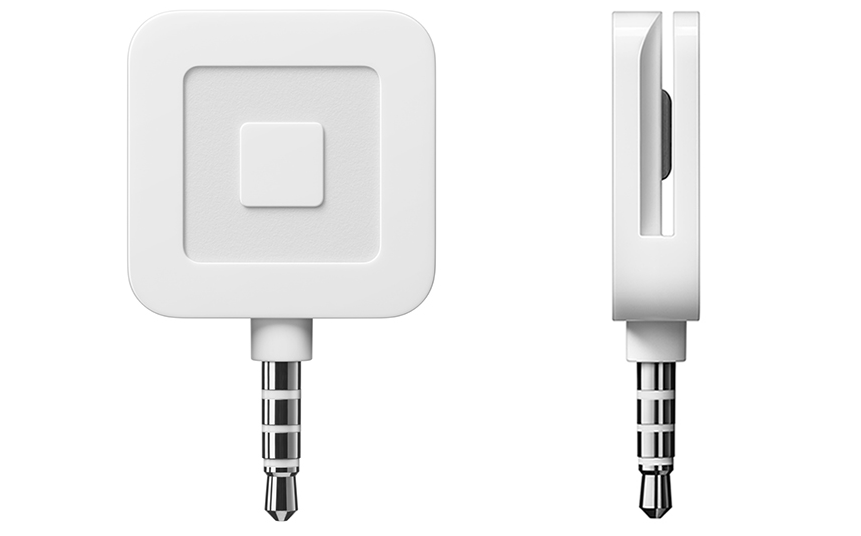
\includegraphics[scale=0.15]{assets/square_reader2.png}\\
  一部の古いクレジットカードでSquareで読み取れない場合はこれを用いる。
  \item iPad\\
  決済を行うのに用いる。
 \end{itemize}
 \subsubsection{使い方}
 \begin{itemize}
  \item クレジットカード
  \begin{itemize}
  \item ICカード
  \begin{enumerate}[手順1]
   \item Square リーダー上部にあるカードスロットに、ICカードのオモテ面を上にしてICチップのある側からカードを挿入する。\\
   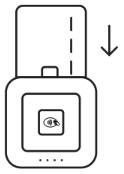
\includegraphics[scale=0.4]{assets/square_insert-card.png}
   \item カードは差し込んだままにし、 Square リーダーから「ピー」と音が鳴って、\\緑色のランプが4つ{\color{green}●●●●}点灯したらカードを取り出す。
   \item お客様にiPadの画面に指でサインをもらい決済を完了する。
  \end{enumerate}
  \item 磁気テープカード\\
  リーダーをiPadのイヤホンジャックに差し込み、磁気テープのみのクレジットカードをスワイプする。
  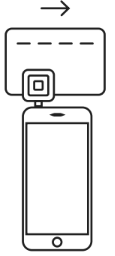
\includegraphics[scale=0.4]{assets/square_slide-card.png}
  \end{itemize}
  \item 電子マネー\\
  交通系IC、QUICPay、iDでの決済
  \begin{enumerate}[手順1]
   \item 「電子マネー」をタップ。
   \item お客様が希望する決済方法を選択。
   \item 青色のランプが4つ{\color{blue} ●●●●}点滅し、画面が「お待ちください。準備をしています。」から「交通系ICカード/iD/QUICPayカードをSquare リーダーにタッチしてください。決済音が鳴るまで動かさないでください。」に変わる。お客様に支払い金額を確認いただき、カードもしくはモバイル端末をSquare リーダーにタッチしてもらう。
   \item POSレジから「ピピッ」と決済音が鳴ったら決済完了。
  \end{enumerate}
 \end{itemize}
 \subsubsection{必要なApp}
 \begin{itemize}
 \item Square POSレジ
 \item 食品レジ(オリジナルApp)
 \end{itemize}
 \begin{itembox}[l]{【オリジナルAppが必要な理由】}
  \begin{itemize}
   \item 現金決済の対応\\
   Square単体では現金決済対応していないが、APIを使用すれば現金決済をSquare上に反映することができる。
   \item 店舗ごとのメニュー対応\\
   Square単体では、同じ場所にある複数店舗に対し別々のメニューを提供することができないので、オリジナルAppを作ることで、店舗ごとにその店舗用のメニューを表示し、またメニューごとにどれだけ注文されたかのデータを記録することができる。
  \end{itemize}
 \end{itembox}
 \subsubsection{食品決済アプリ}
  \begin{enumerate}
   \item 目的\\
   食品などの支払いで電子マネーを使用できるようにするとともに、現金も含めた全ての支払いを管理する目的。
   \item 必要物品
   \begin{itemize}
   \item iPad(各店舗につき1台)$\cdots$アプリケーション
   \item Square Reader$\cdots$カードの読み取り用ハードウエア
   \end{itemize}
   \item マニュアル
   \begin{enumerate}
   \item 注文されている商品を入力する\\
   表示されている商品が別店舗の場合は、左上の設定ボタンから店舗を変更できる。\\
   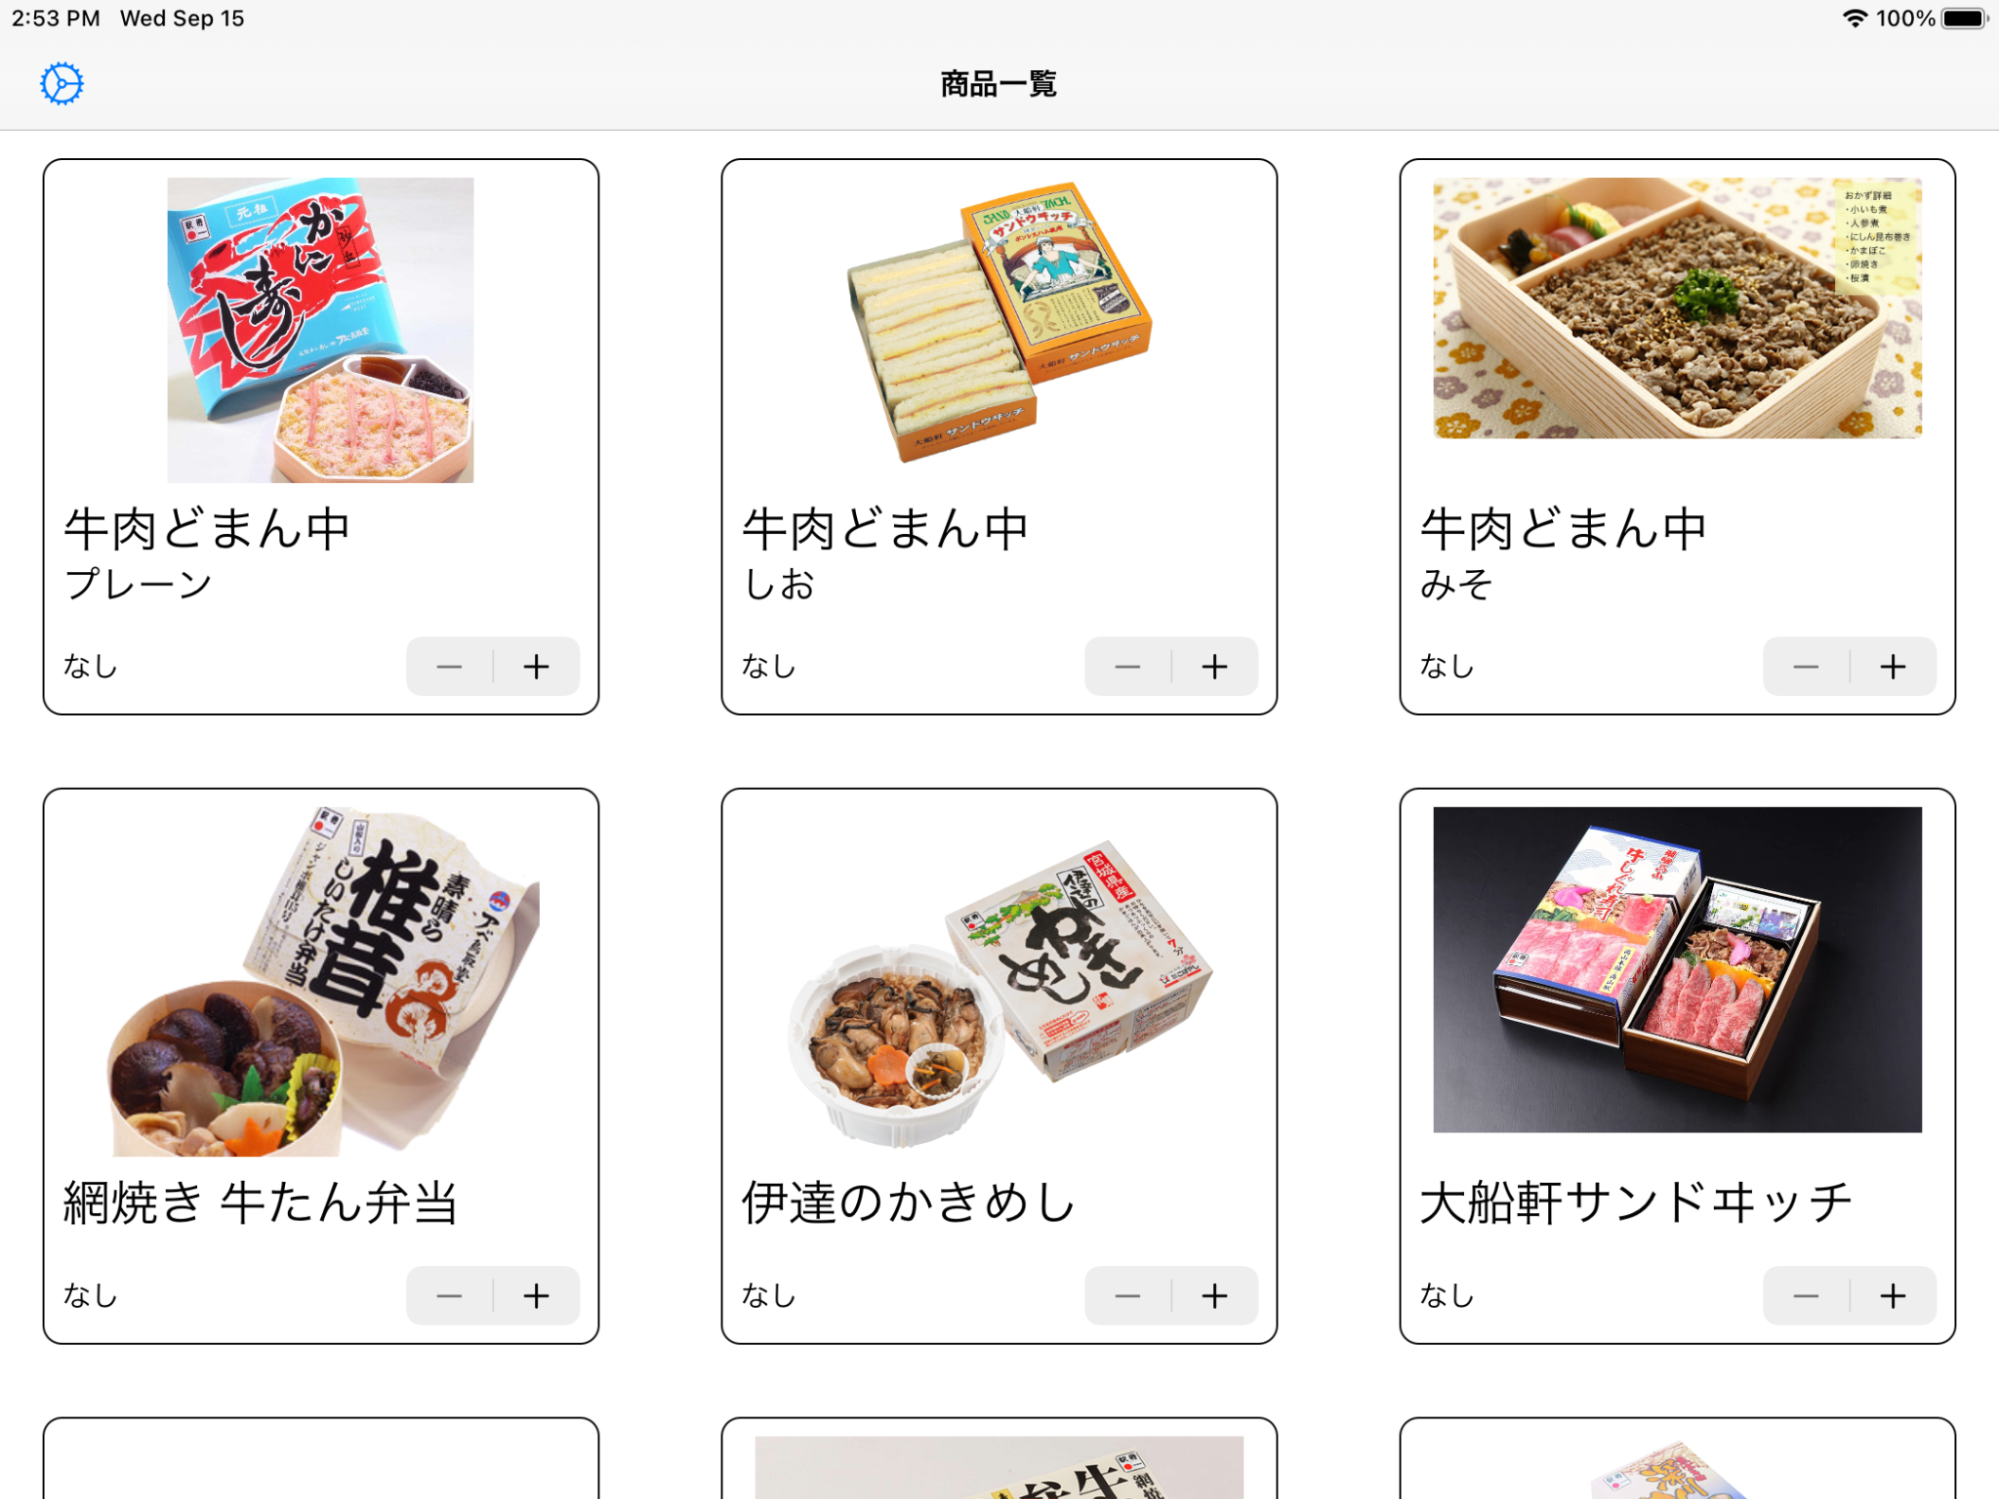
\includegraphics[scale=0.15]{assets/square_top-interface.png}
   \item 合計金額をお客様に伝えて、現金決済と電子決済のどちらにするか聞く\\
   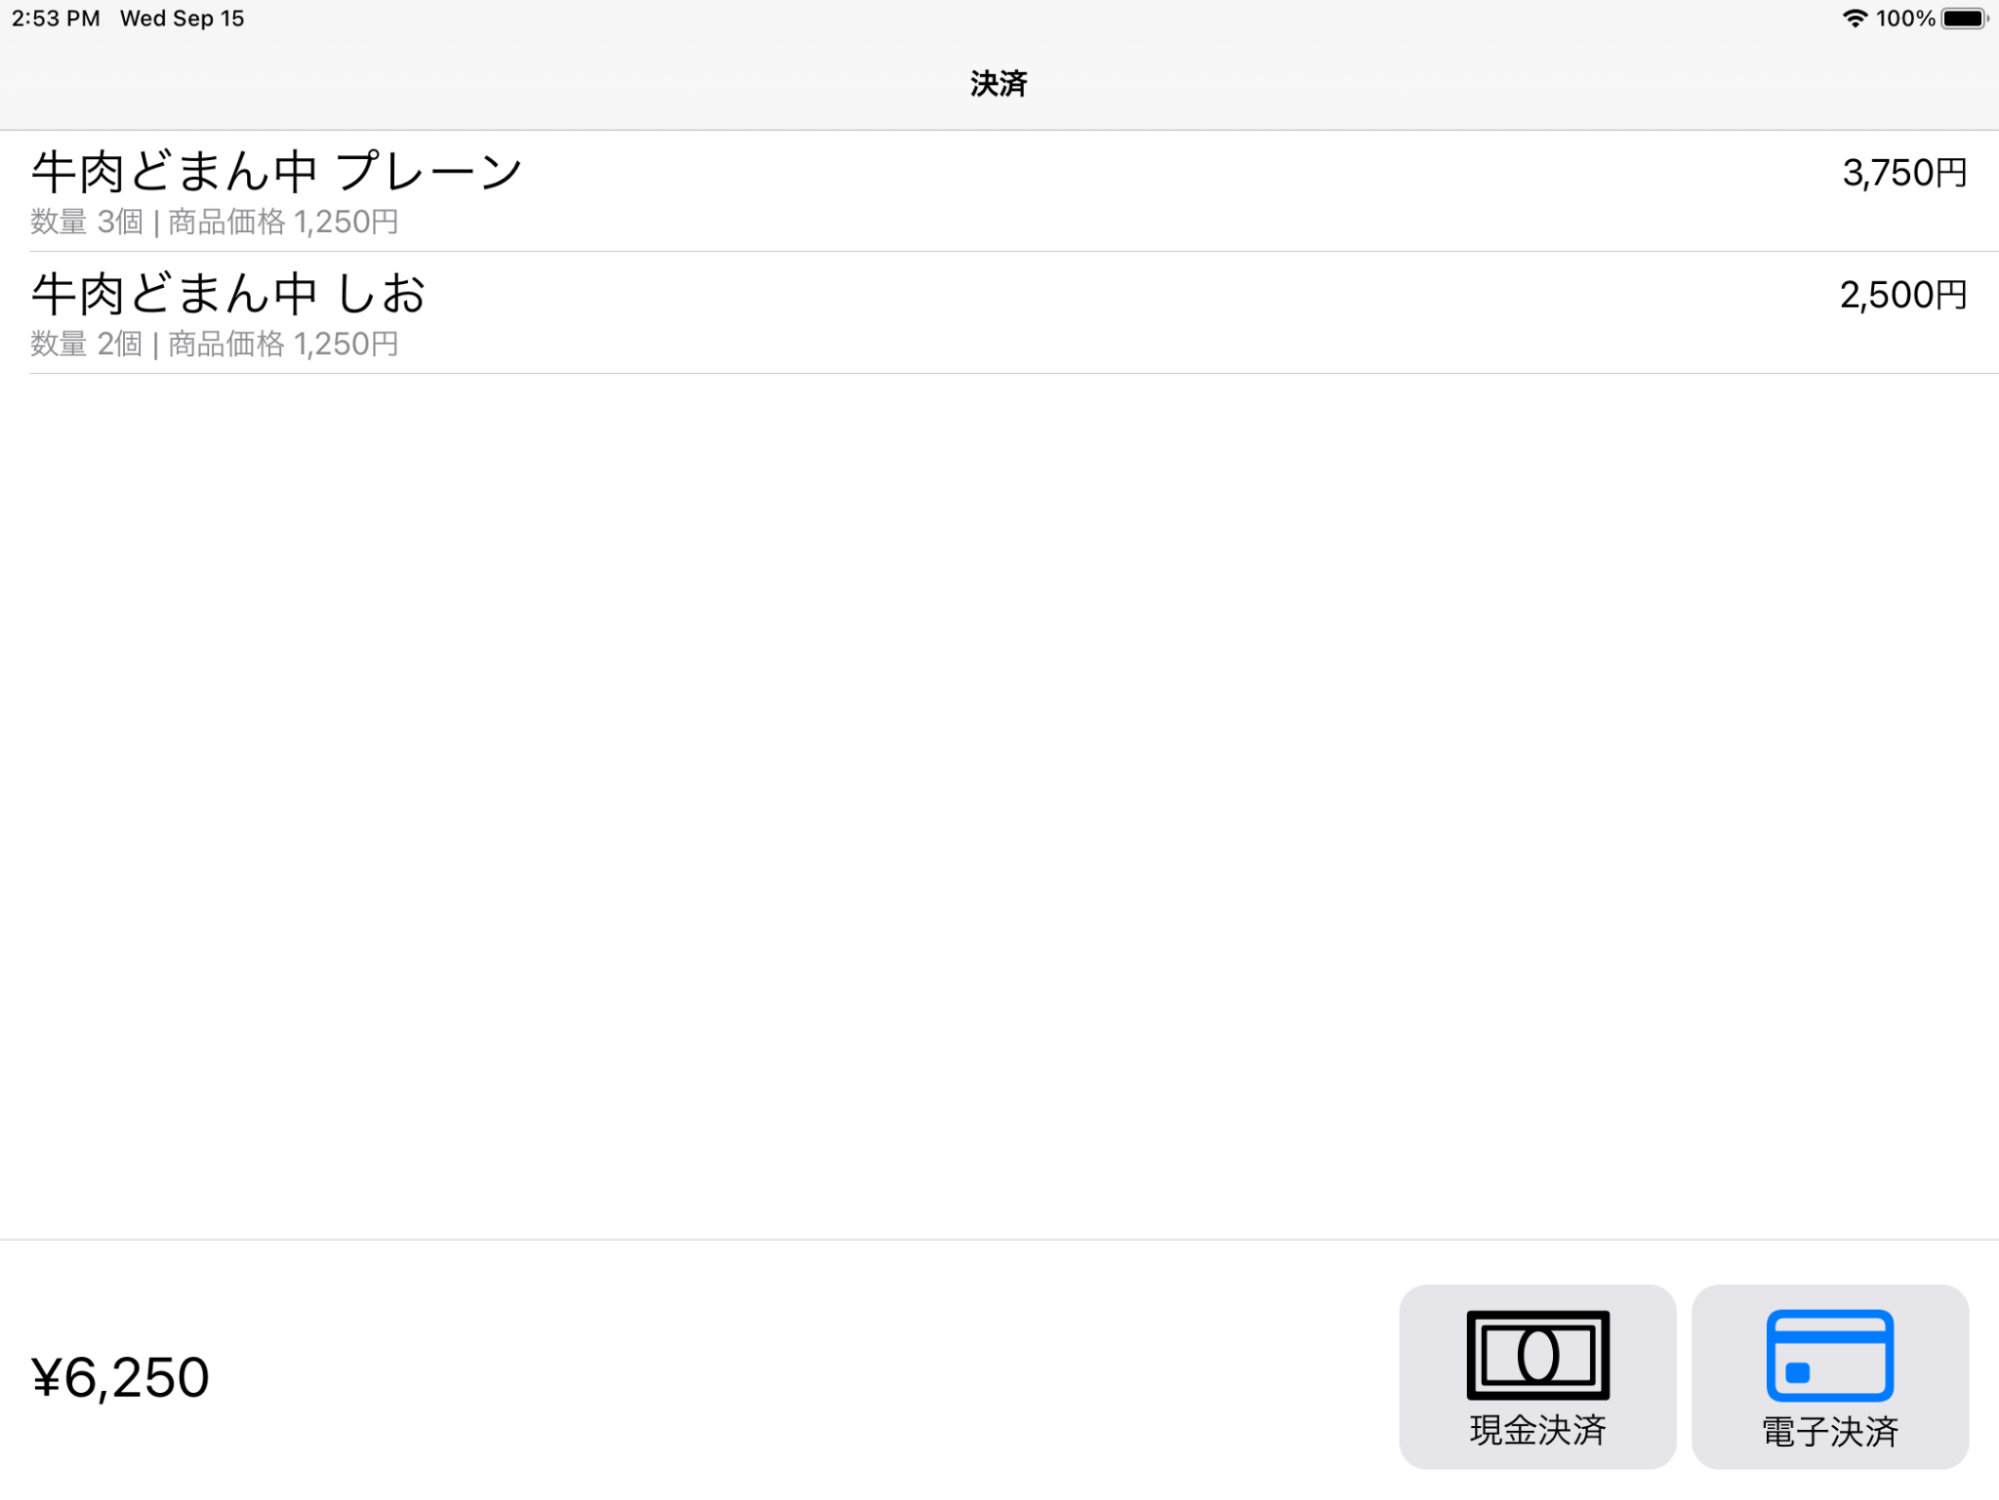
\includegraphics[scale=0.15]{assets/square_second-interface.png}
   \item 右下のどちらかのボタンを押すと、Square POS レジアプリに飛ぶ\\
   事前に伝えられたパスワードを入力する。\\
   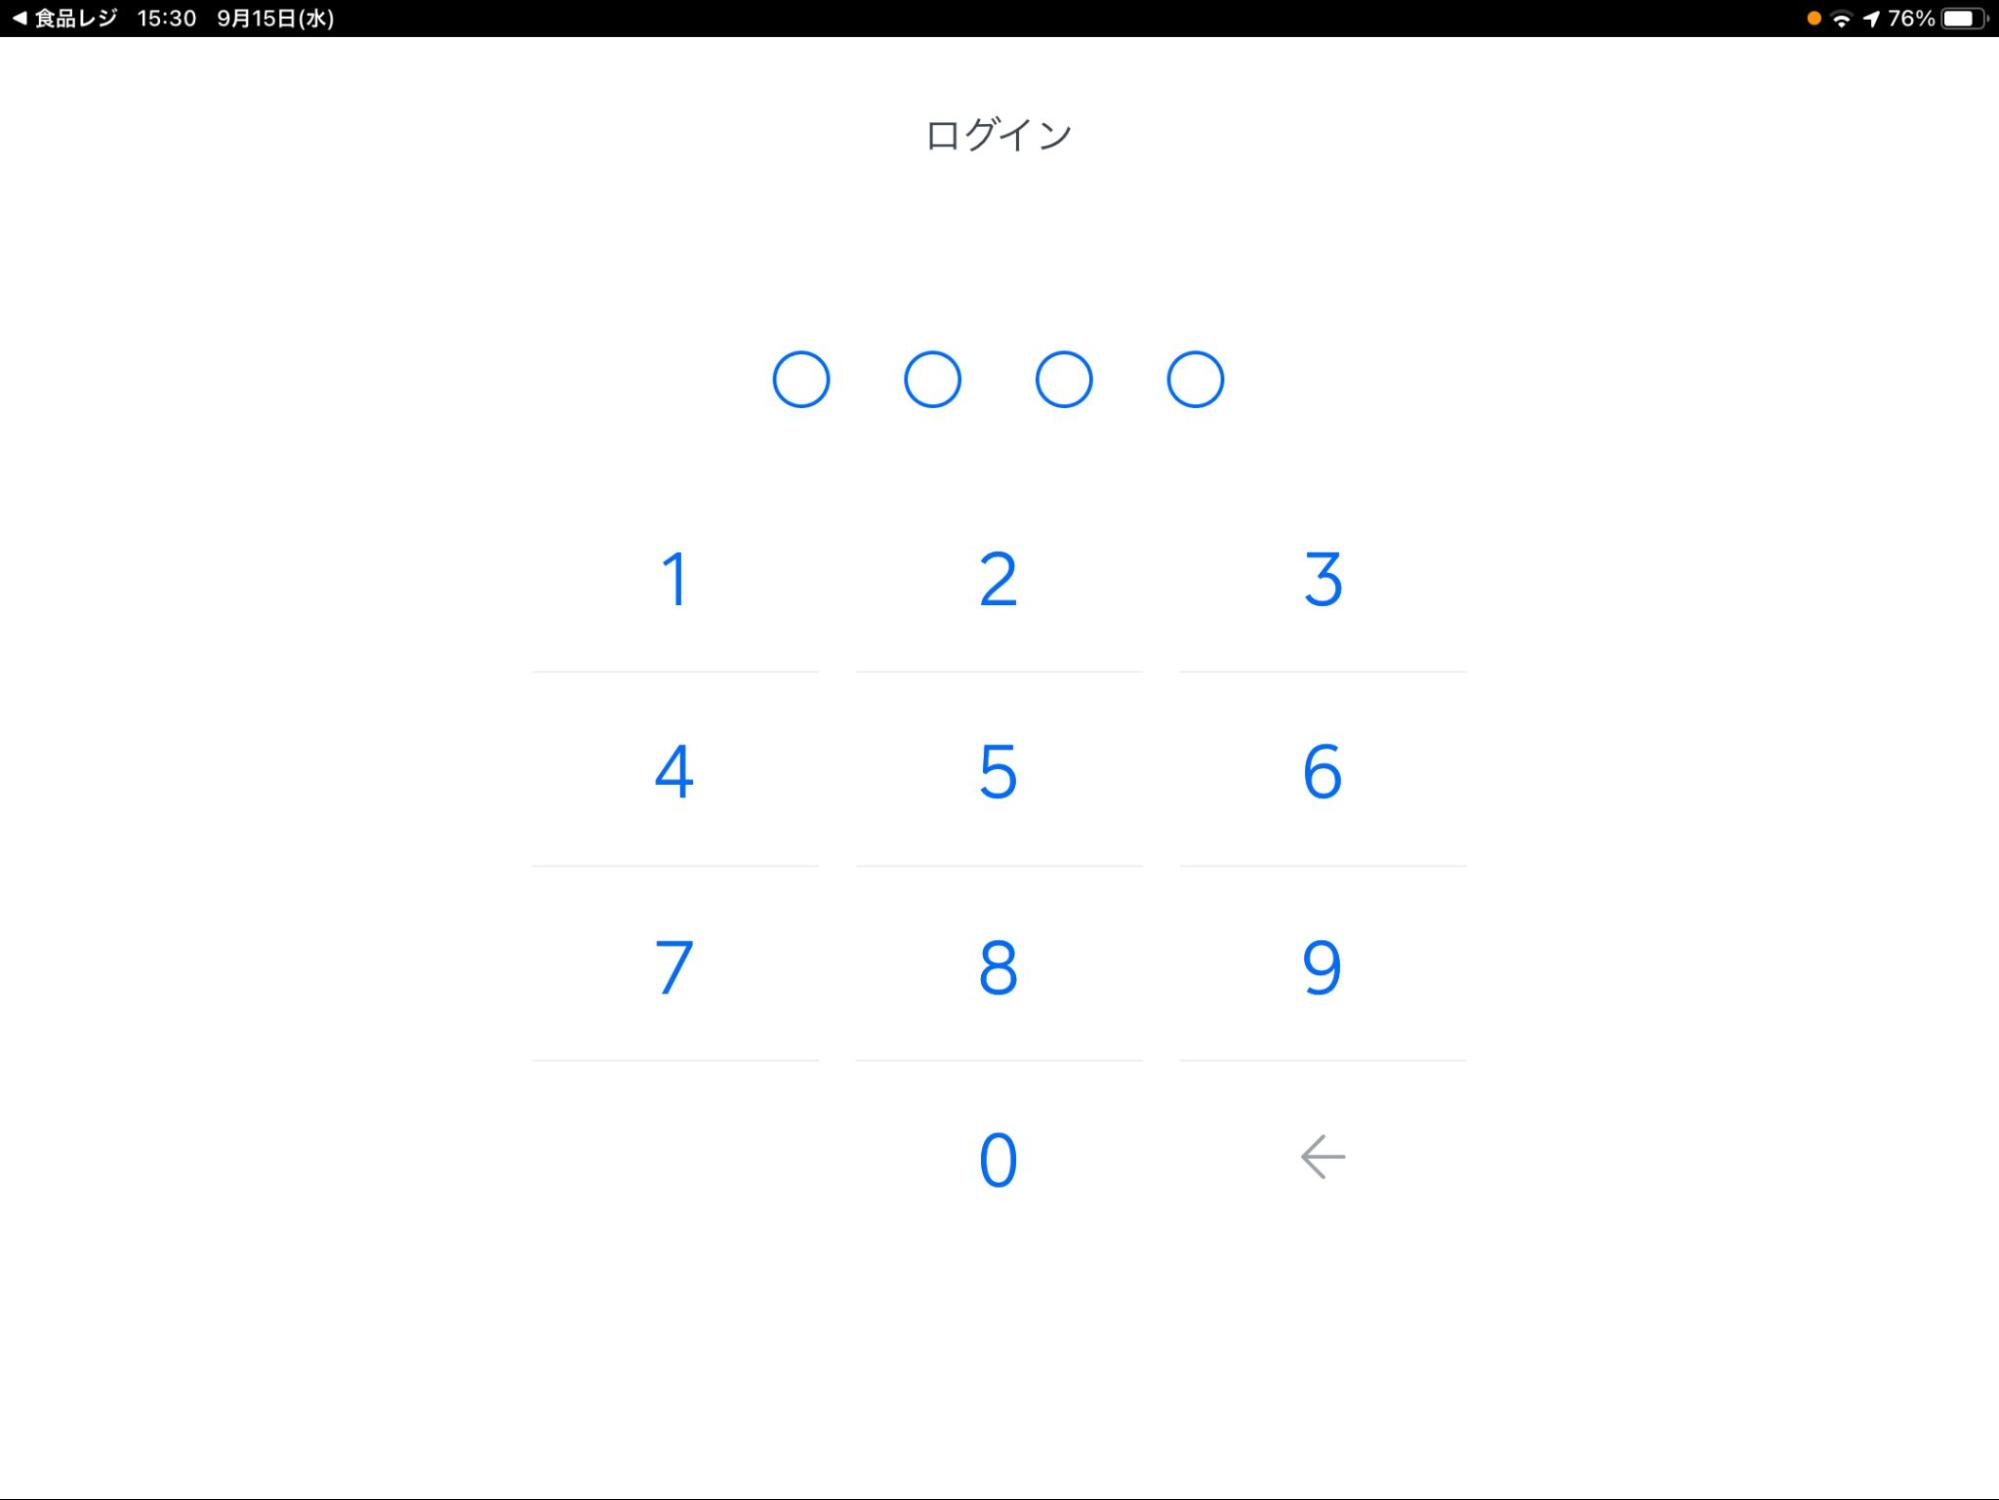
\includegraphics[scale=0.2]{assets/square_password-keypad.jpg}
   \item 決済
    \begin{enumerate}
     \item 現金決済\\
     お預かり金額を選ぶ。\\
     選択肢にない場合は、「カスタム」を押して入力する。\\
     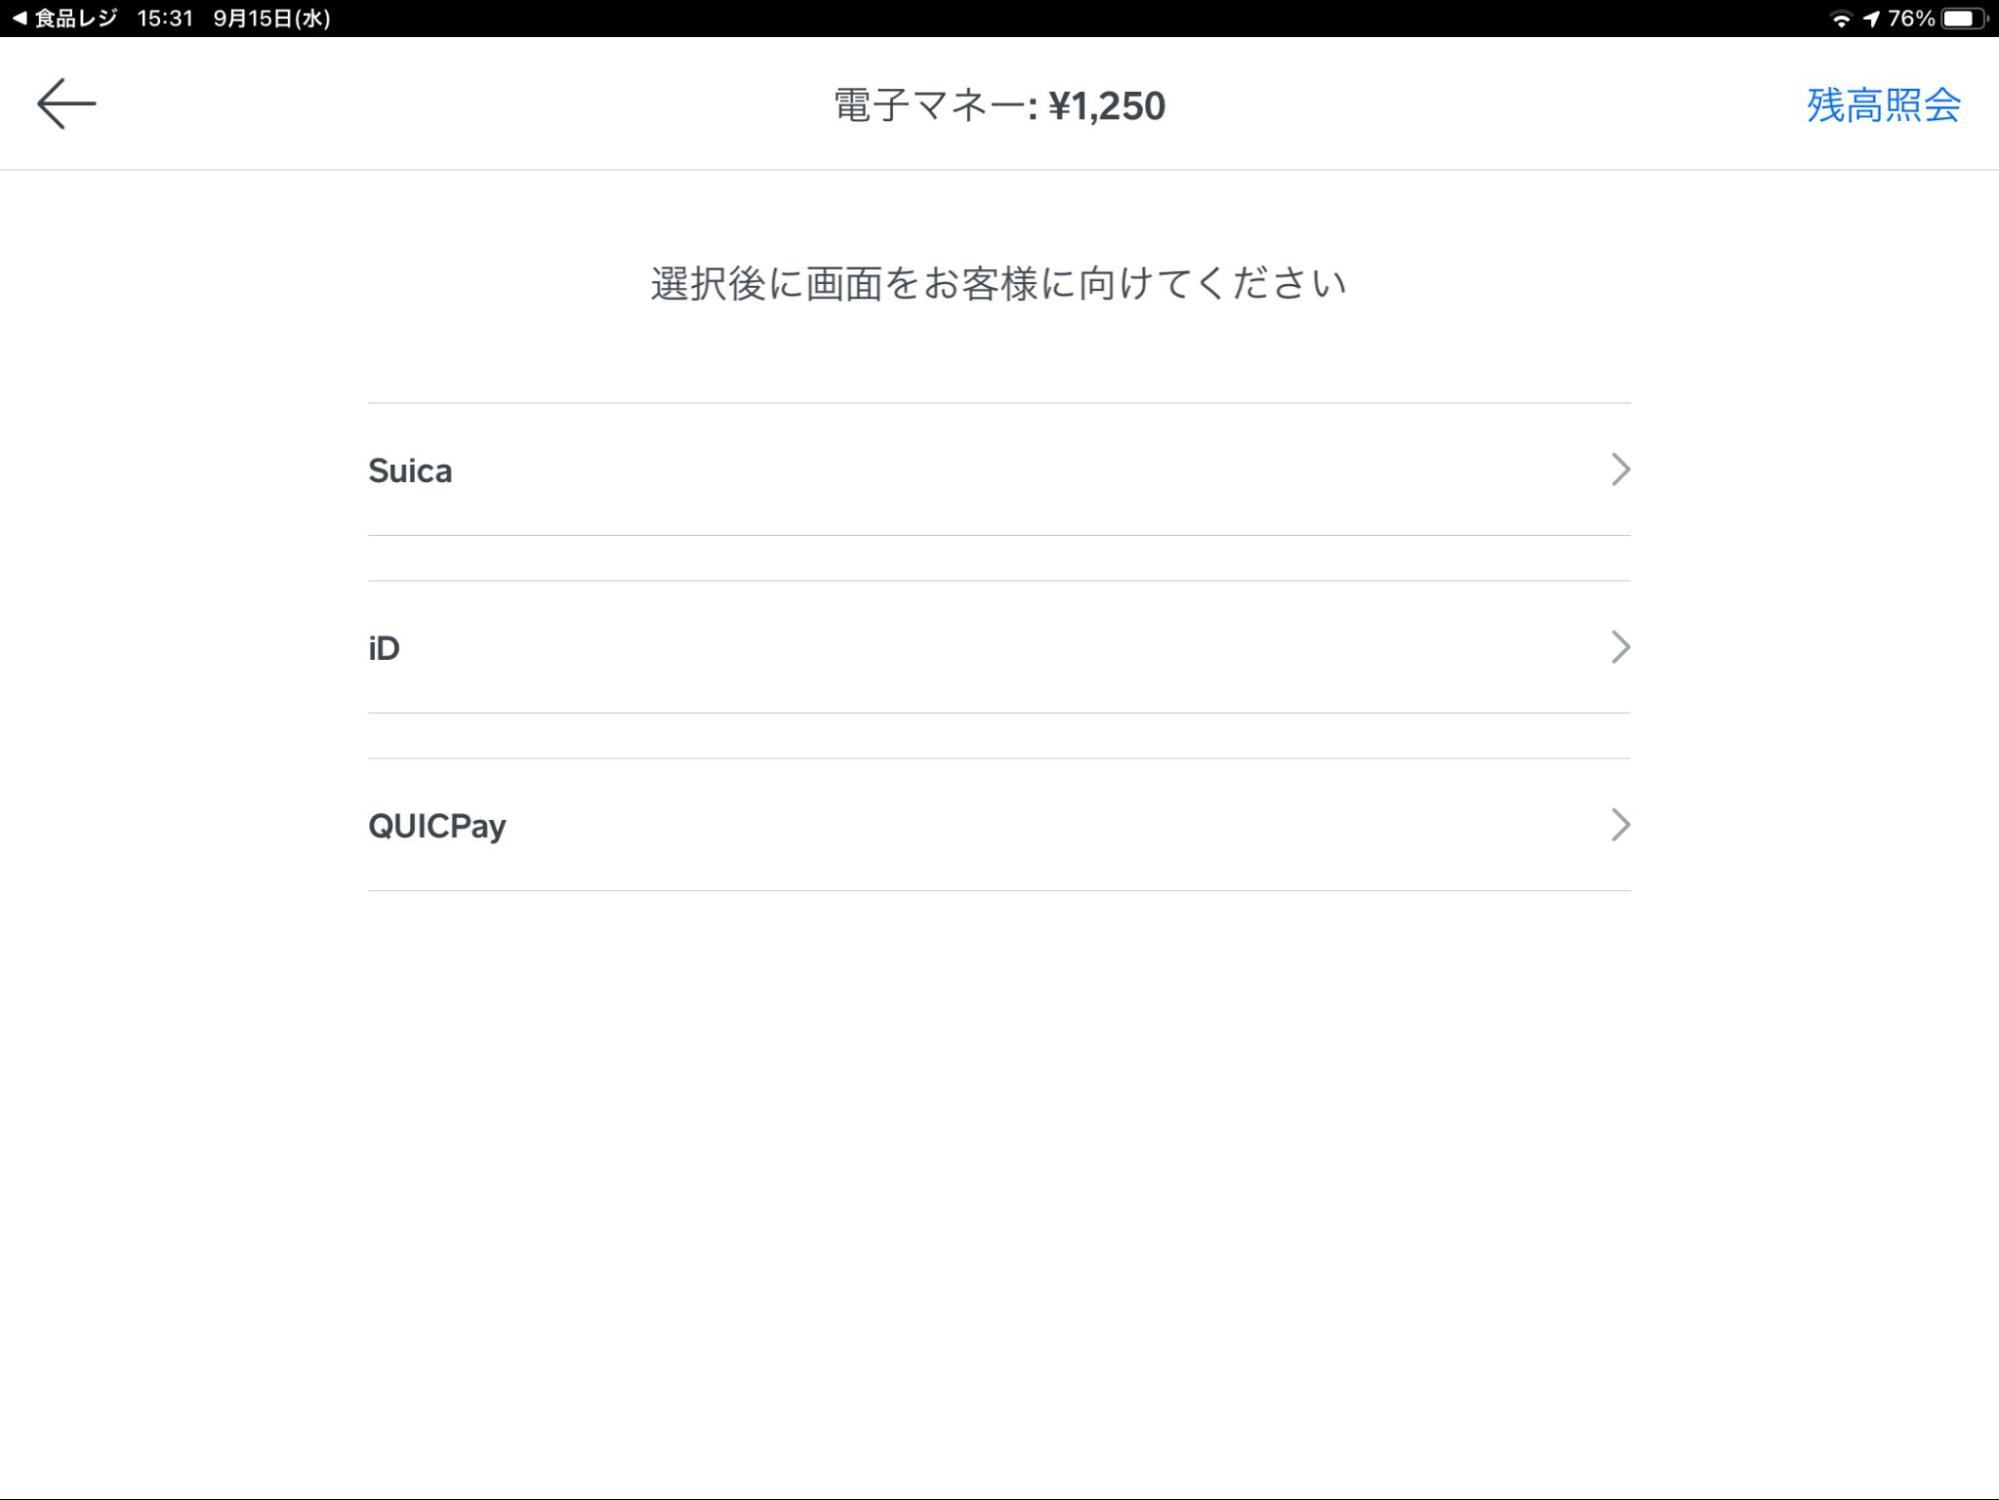
\includegraphics[scale=0.2]{assets/square_e-payment_selection.jpg}\\
     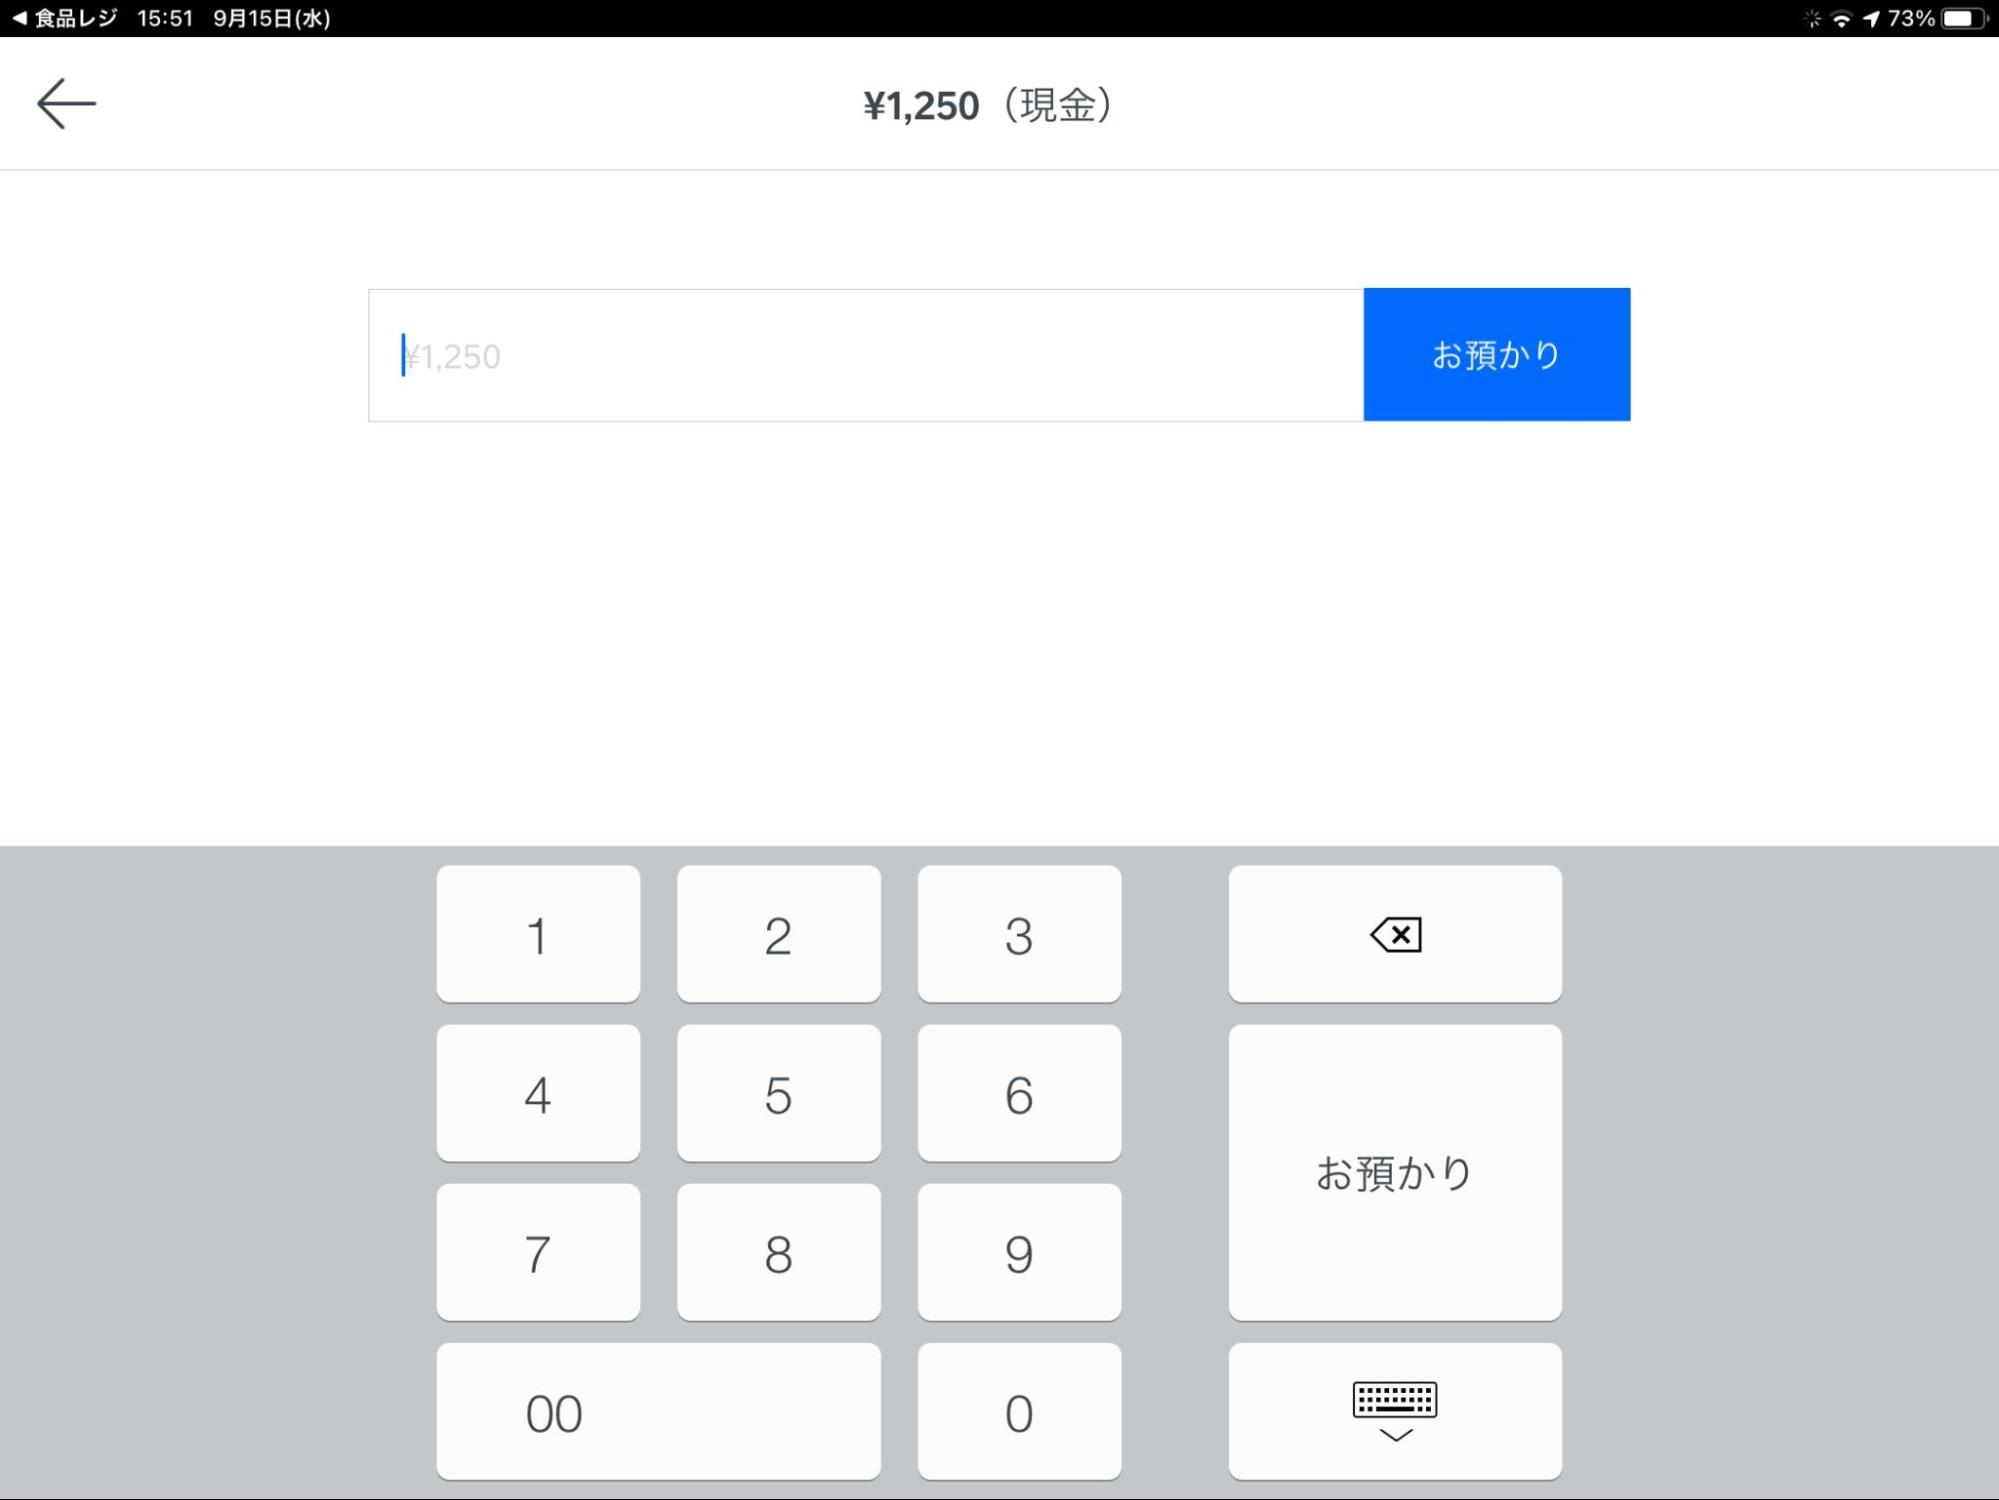
\includegraphics[scale=0.2]{assets/square_cash-payment-custom.jpg}
     \item 電子決済\\
     決済方法を聞いて選んで、カードリーダーにかざしてもらう。\\
     画面をお客様に向ける必要はない。\\
     決済が完了すると、元のアプリに戻る。\\
     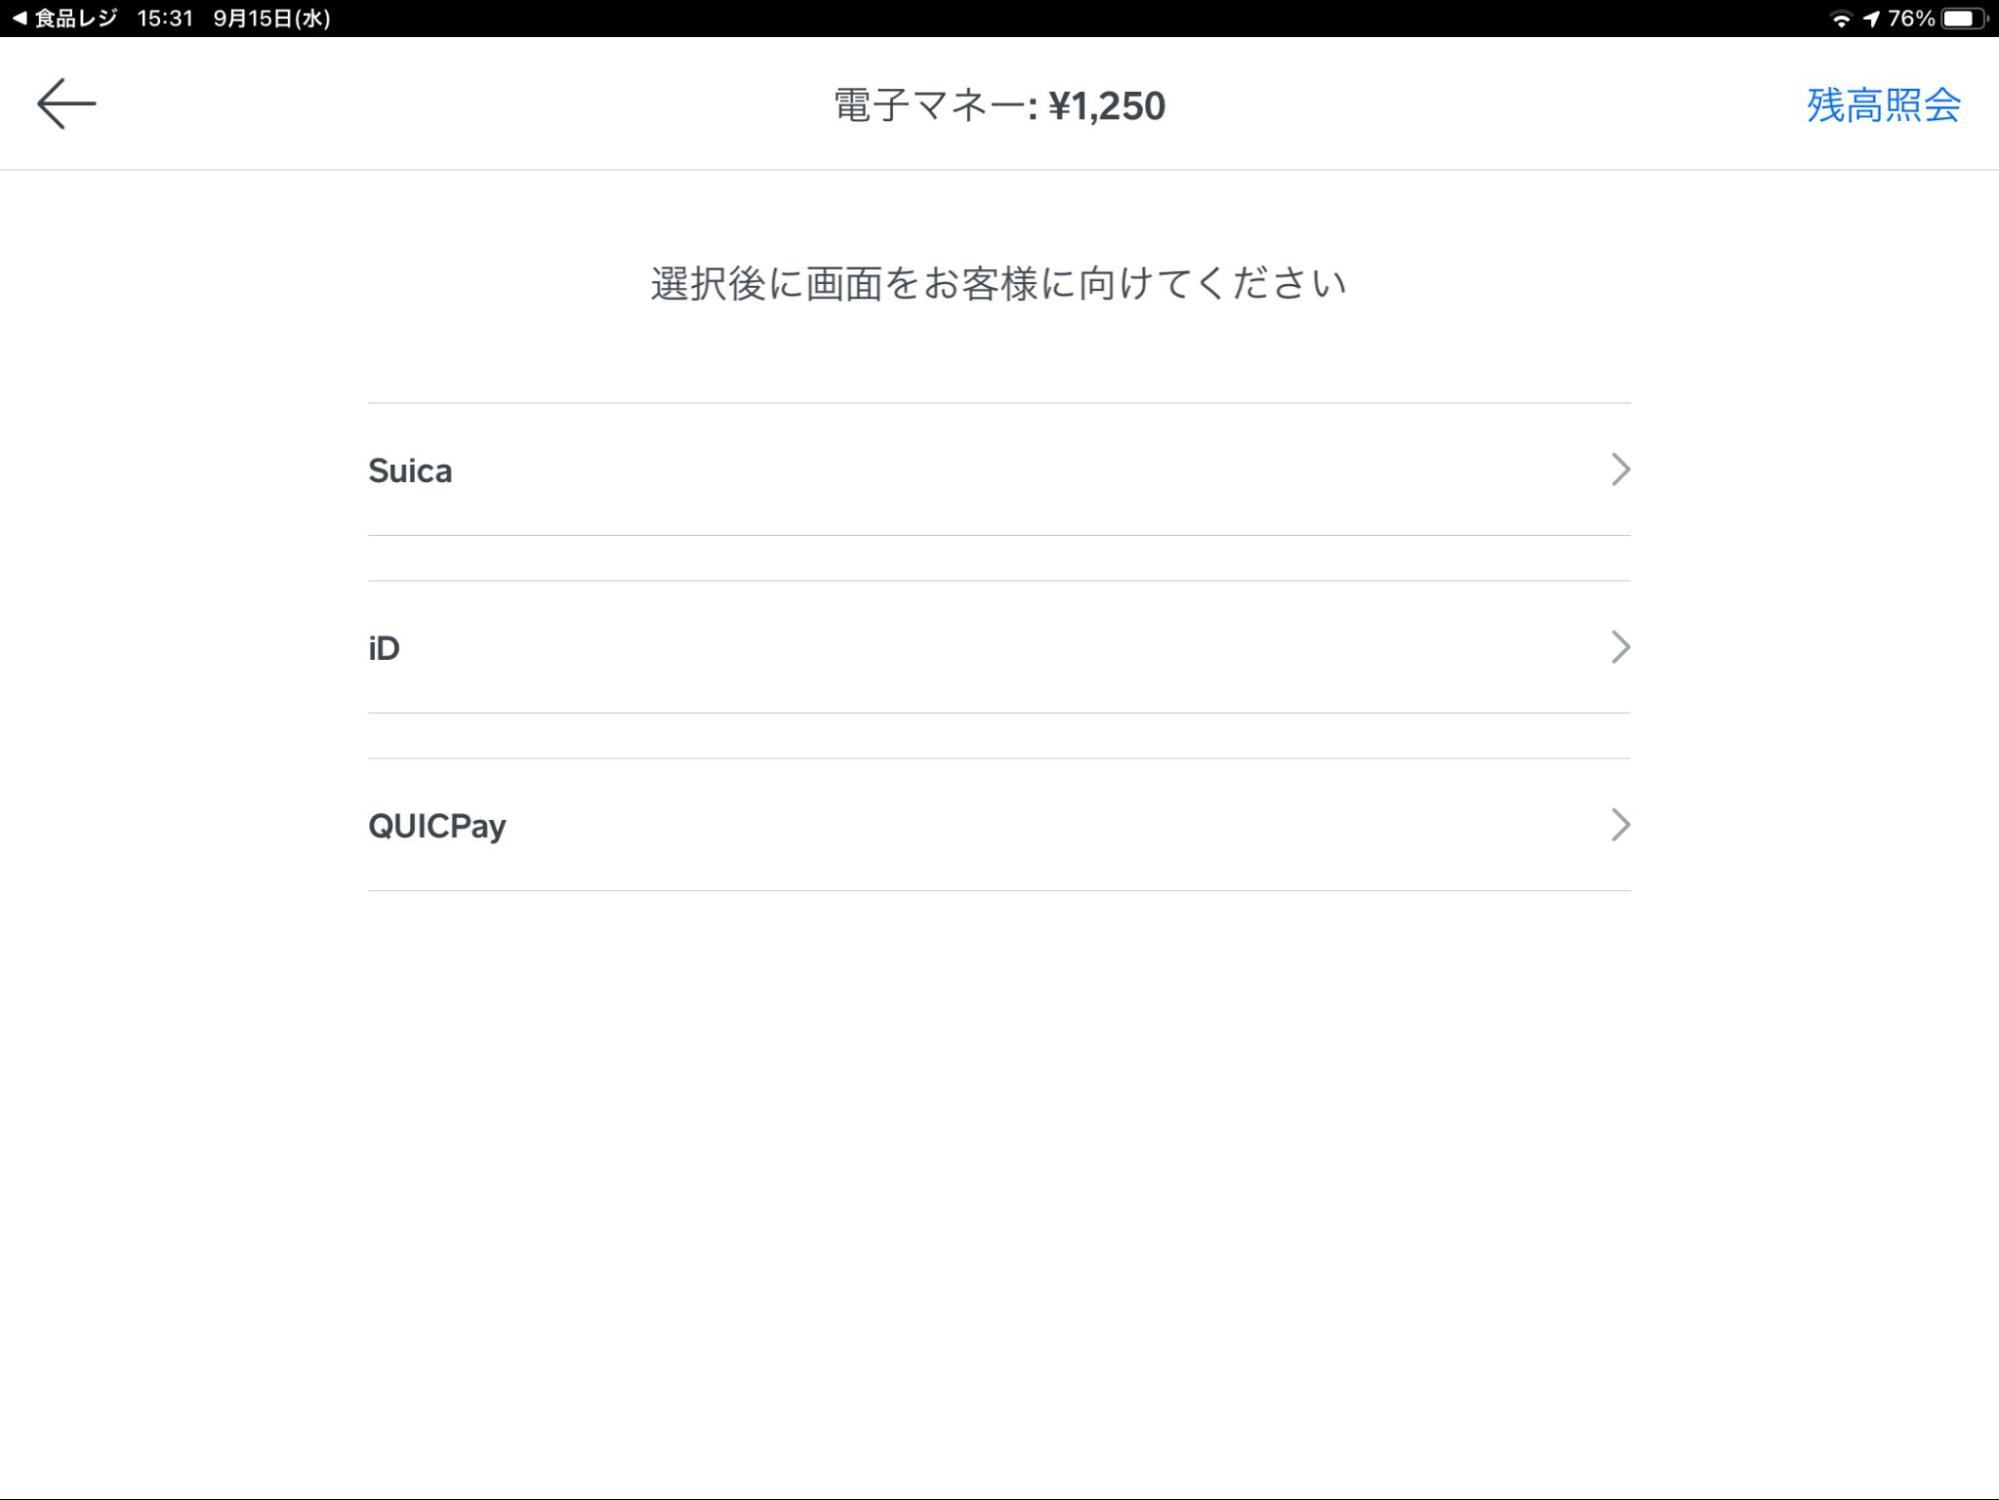
\includegraphics[scale=0.2]{assets/square_e-payment_selection.jpg}\\
     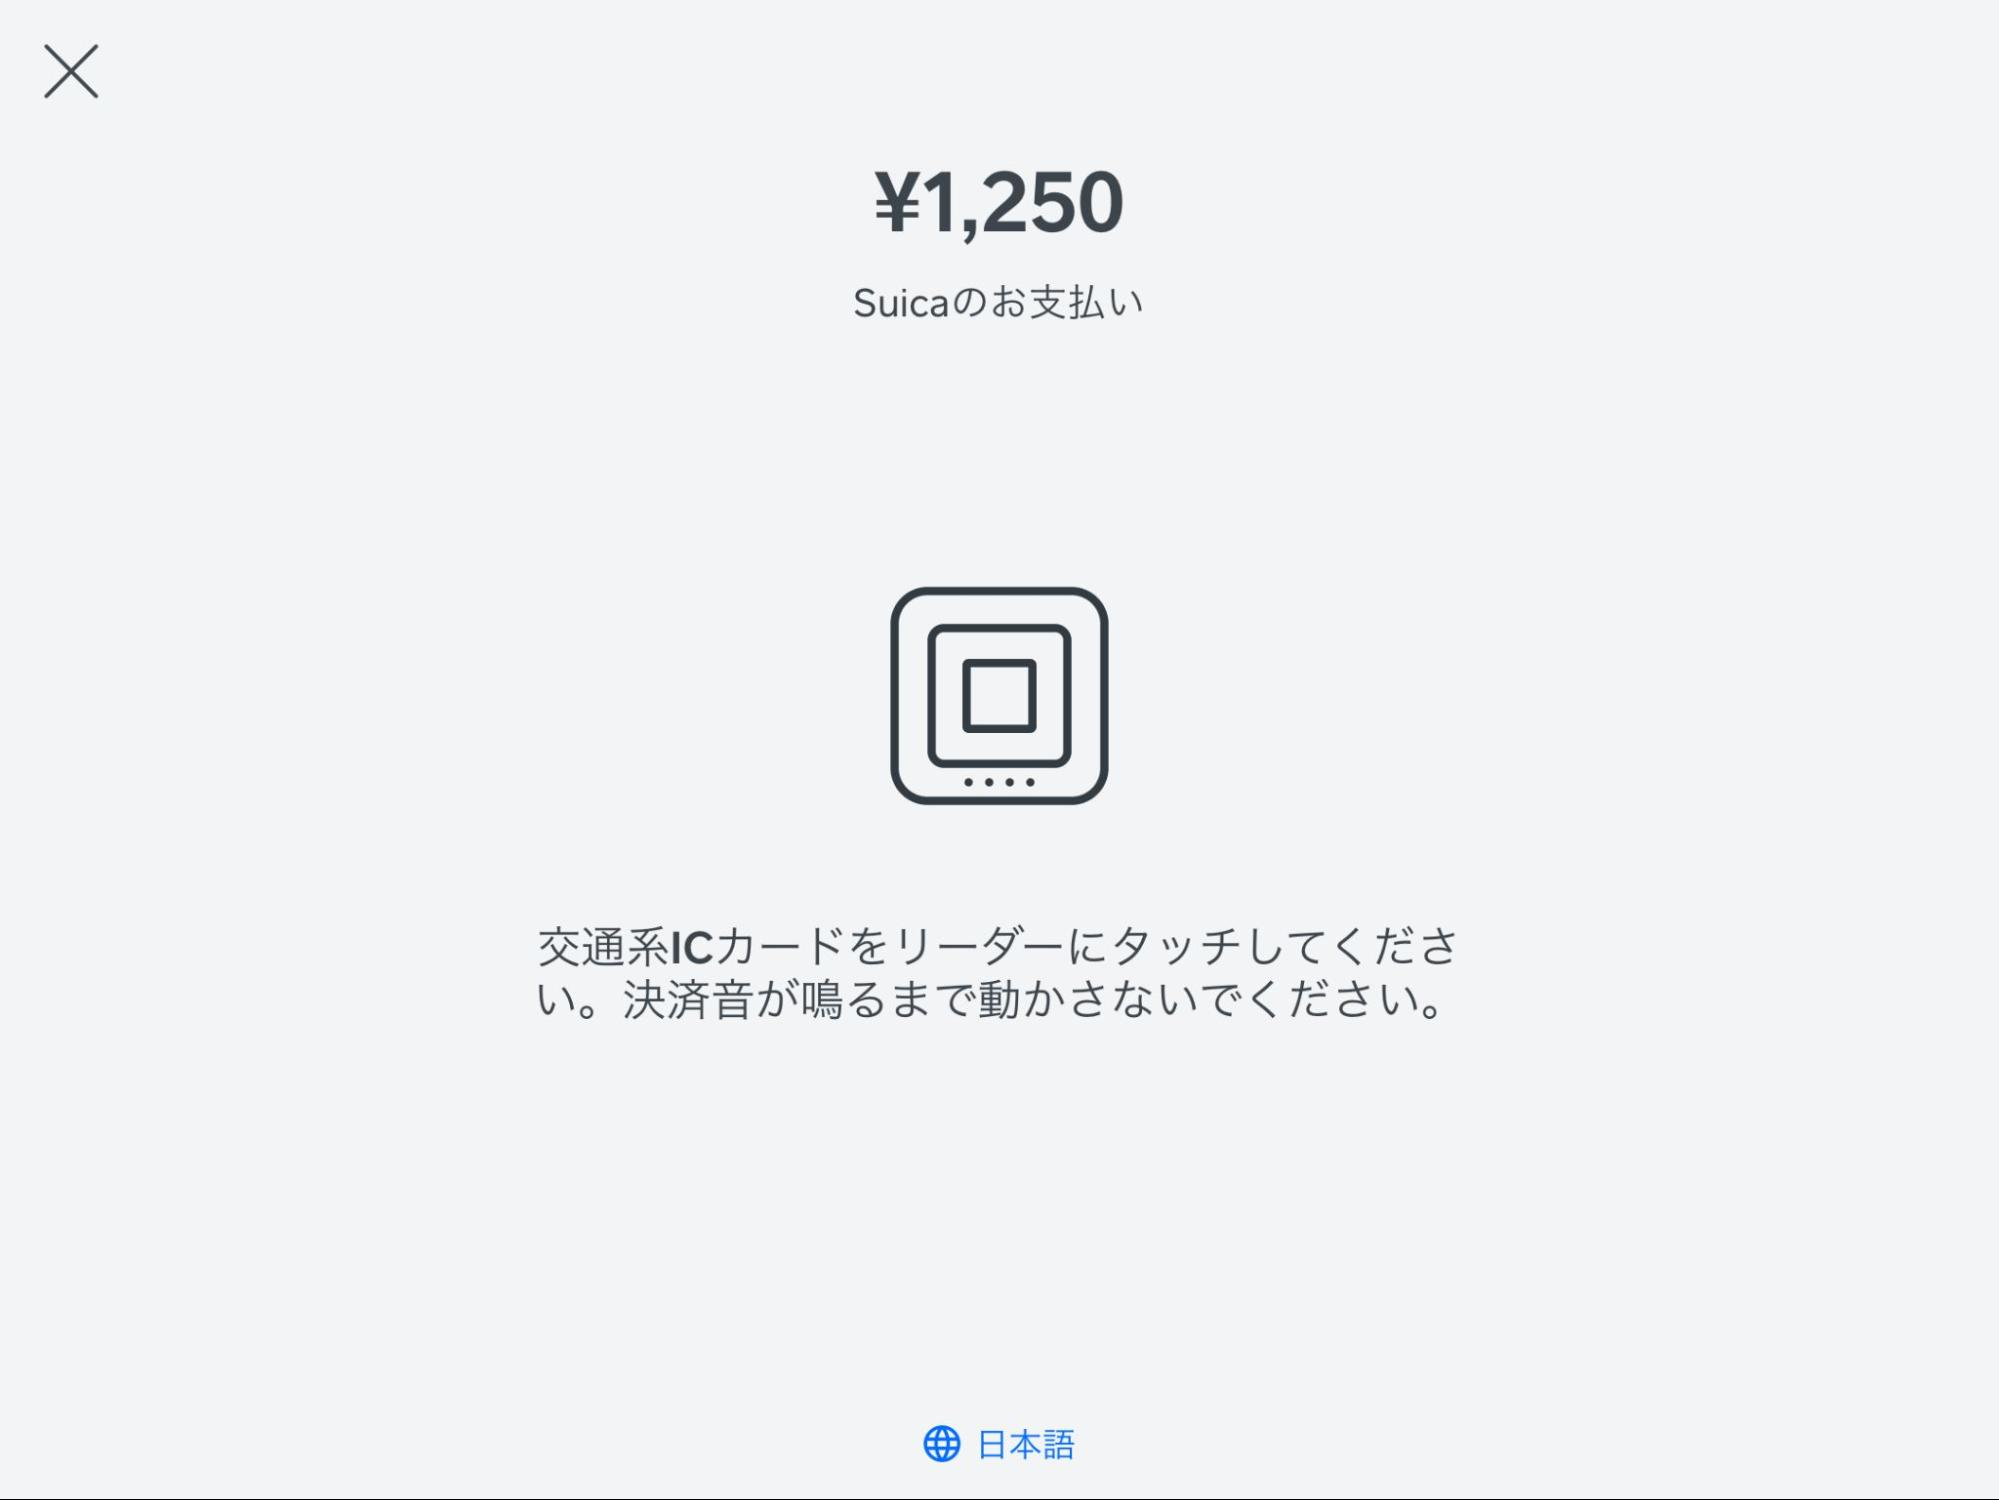
\includegraphics[scale=0.2]{assets/square_e-payment_scan.jpg}
    \end{enumerate}
   \end{enumerate}
  \end{enumerate}

\newpage
\subsection{QRコードシステム}
入場システム、展示団体入退場管理システム、食品予約システム、講堂予約システムをまとめたシステム。
\subsubsection{グループID}
グループIDは予約の申し込み時にフォームに回答したお客様にメールにて配布されたIDで、グループを識別するものである。グループIDには「姓(カタカナ)」「人数」「ご予約時間帯(日/午前・午後)」「枠」が紐づけられている。姓は代表者のものになっている。
IDの形式は以下の通りである。(覚える必要はない。)
\begin{screen}
 \begin{center}
 {\huge \# AB-CCCC}\\
 \end{center}
A$\cdots$日付(0~3)1~3は1~3日目を表す。0は全ての日付で入場可(在校生用)。\\
B$\cdots$時間帯(0,1)0は前半の部、1は後半の部。\\
C$\cdots$番号(0000〜9999)
\end{screen}
 このグループIDは予約確認のメールにQRコードとして添付してあるため、主にカメラによる入力をする。なお、一応番号による入力もある。お客様に伝えるときは「グループID」を見させてもらうのではなく「予約完了メール」を見させてもらうようにする方がわかりやすい。使用するのは主に「入場システム」と「個人ID再発行システム」である。
 \subsubsection{個人ID}
 個人IDは入場時に印刷されるシールに記載しており、パンフレットの裏表紙に貼られているIDで、個人を識別するものである。個人IDには「グループID」「行動履歴」が紐づけられている。
 IDの形式は以下の通りである。(覚える必要はない。)
 \begin{screen}
 \begin{center}
 {\huge \# AA-AAAA-B}\\
 \end{center}
A$\cdots$グループIDそのまま。\\
B$\cdots$番号(0~5)0が代表者。
\end{screen}
この個人IDは、パンフレット裏のシールにQRコードとして記載されているため、主にカメラによる入力をする。なお、一応番号による入力もある。お客様に伝えるときは「個人ID」を見させてもらうのではなく「パンフレット裏」または「入場時にもらったシール」を見させてもらうようにする方がわかりやすい。使用するのは「入場システム」と「個人ID再発行システム」以外のすべてのシステムである。
\subsubsection{全体の概形図}
 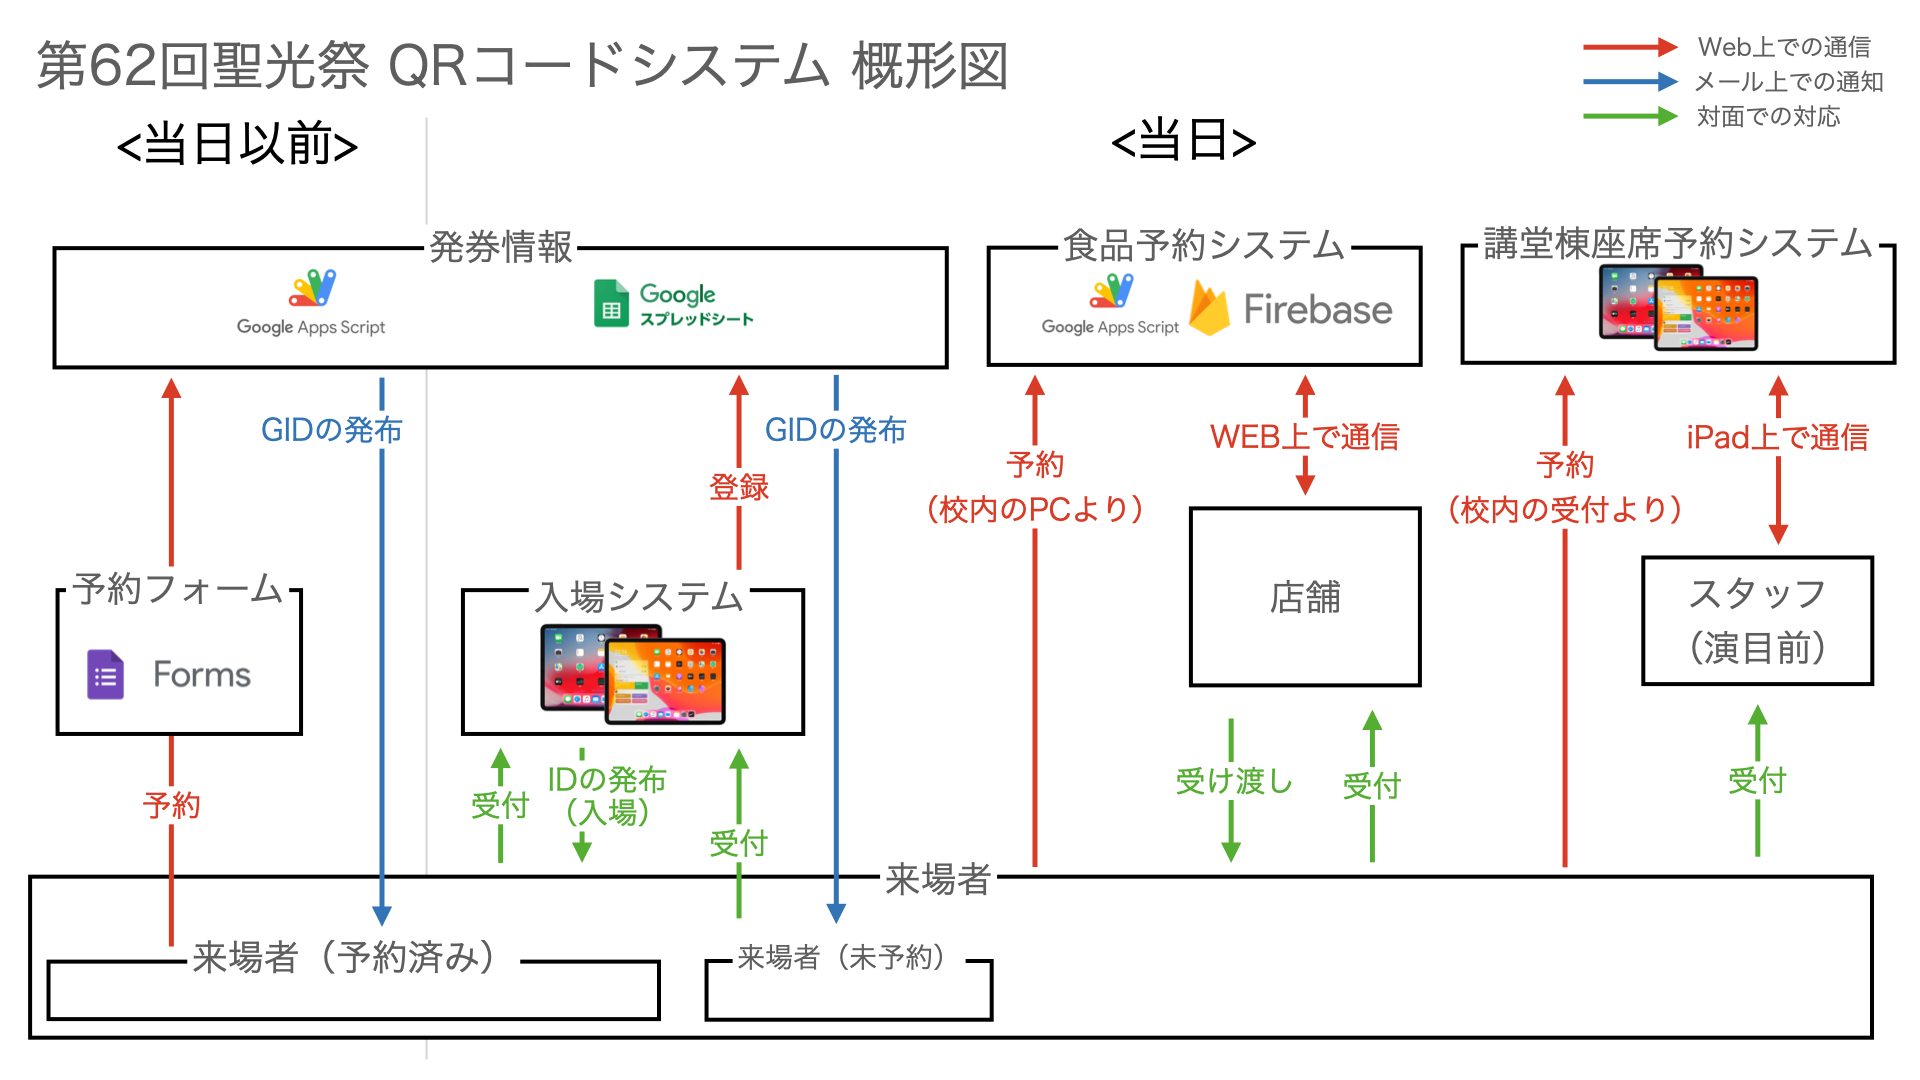
\includegraphics[scale=0.15]{assets/qrcode-system-first-look.png}
\subsubsection{設立のプロセス}
\begin{itemize}
 \item[1月] 三枝が新宿のAppleStoreで商品の受け取りに行った際、\\AppleStoreの入場制限のシステムを見て、「これ聖光祭に導入できそうじゃね?」と思う。
 \item[2月上旬] 実行委員長の大下に提案\\
 画像は下から順。\\
 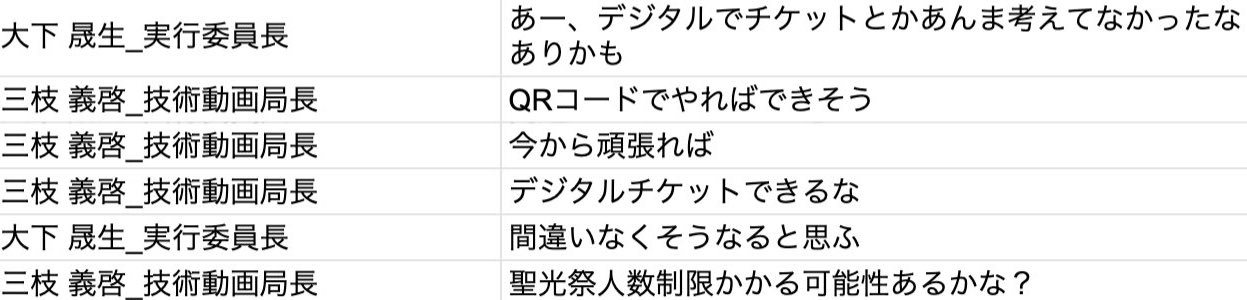
\includegraphics[scale=0.3]{assets/QR_the_beginning.jpg}
 \item[2月下旬] プロジェクト始動。執行部・外務部門間で入場方式をどのようにするかについて検討。この際は入場時にQRコードをスキャンするだけで、特に入場後にQRコードを配布する予定ではなかった。\\当時は、ターム制で入場時間が、午前午後より細かく分けられていた。また、それぞれの時間帯に分けて色別のリストバンドが配られた。
 \item[5月] 入場システムの機能に展示団体入退場管理、食品予約、講堂予約の機能を追加。また、いくつかのプロトタイプも作られた。
 \item[6月] 最終仕様決定。\\予算的にリストバンドが実現不可能とわかり、シールをパンフレットに貼り付ける形に変更した。\\QRコードシステムと総称がつけられた。
 \item[7月] プリンター、iPad発注。システム開発を再開。プリンターがなくてもできるところはできる限り行った。\\システムに関して、飯岡先生と相談。ターム制ではなく、単に午前午後で分けるように決まった。受験生枠に関しての調整。
 \item[8月中旬] iPad到着/セットアップ。Apple IDの発行。アプリのインストール。
 \item[8月下旬] プリンター到着。実機テスト開始。
 \item[9月中旬] QRコードシステム説明会。来場者の情報確定。
 \item[9月下旬] メール送信開始。
 \item[10/1] 台風で延期になったため、システムの最終調整を行なった。
\end{itemize}
\subsubsection{失敗した理由}
 \begin{itemize}
  \item スプレッドシートの「型」\\
  スプレッドシートにもStringやIntといった型が存在する。聖光祭当日に、大下が三枝の許可を得て動作確認用のサンプルデータをiOS版のスプレッドシートAppで追加したところ、型が狂ってしまい、iPadアプリケーションが落ちてしまった。結局、スプレッドシートを復元しないと解決せず、失敗した。
  \item ポケットWi-Fiの限界\\


 \end{itemize}
\subsubsection{改善点}
\subsection{入場システム}
\subsubsection{目的}
予約したお客様の受付を行い、入場の管理をし、「個人ID」の発行を目的としたiPadアプリケーションである。
\subsubsection{必要物品}
 \begin{itemize}
 \item iPad(1レーンにつき1台)$\cdots$アプリケーションの実行
 \item 感熱式ラベルプリンター(1レーンにつき1台)$\cdots$個人IDシールの印刷
 \item パンフレット(1人につき1部)
 \item 延長コード$(10m\times1,20m\times2,30m\times2)$ $\cdots$プリンターに電源を供給する用
 \item 時計(任意) $\cdots$時間がわかればいい。iPad内蔵のものでもOK。
 \end{itemize}
\subsubsection{マニュアル}
 接客マニュアルについては外務部門マニュアルを参照すること。
 \begin{enumerate}
  \item QRコードを読み込む\\
  カメラの枠内にQRコードをおさめ、気持ち長めに静止させる。\\
  QRコードが読み込めない場合には、手動入力もできる。\\
  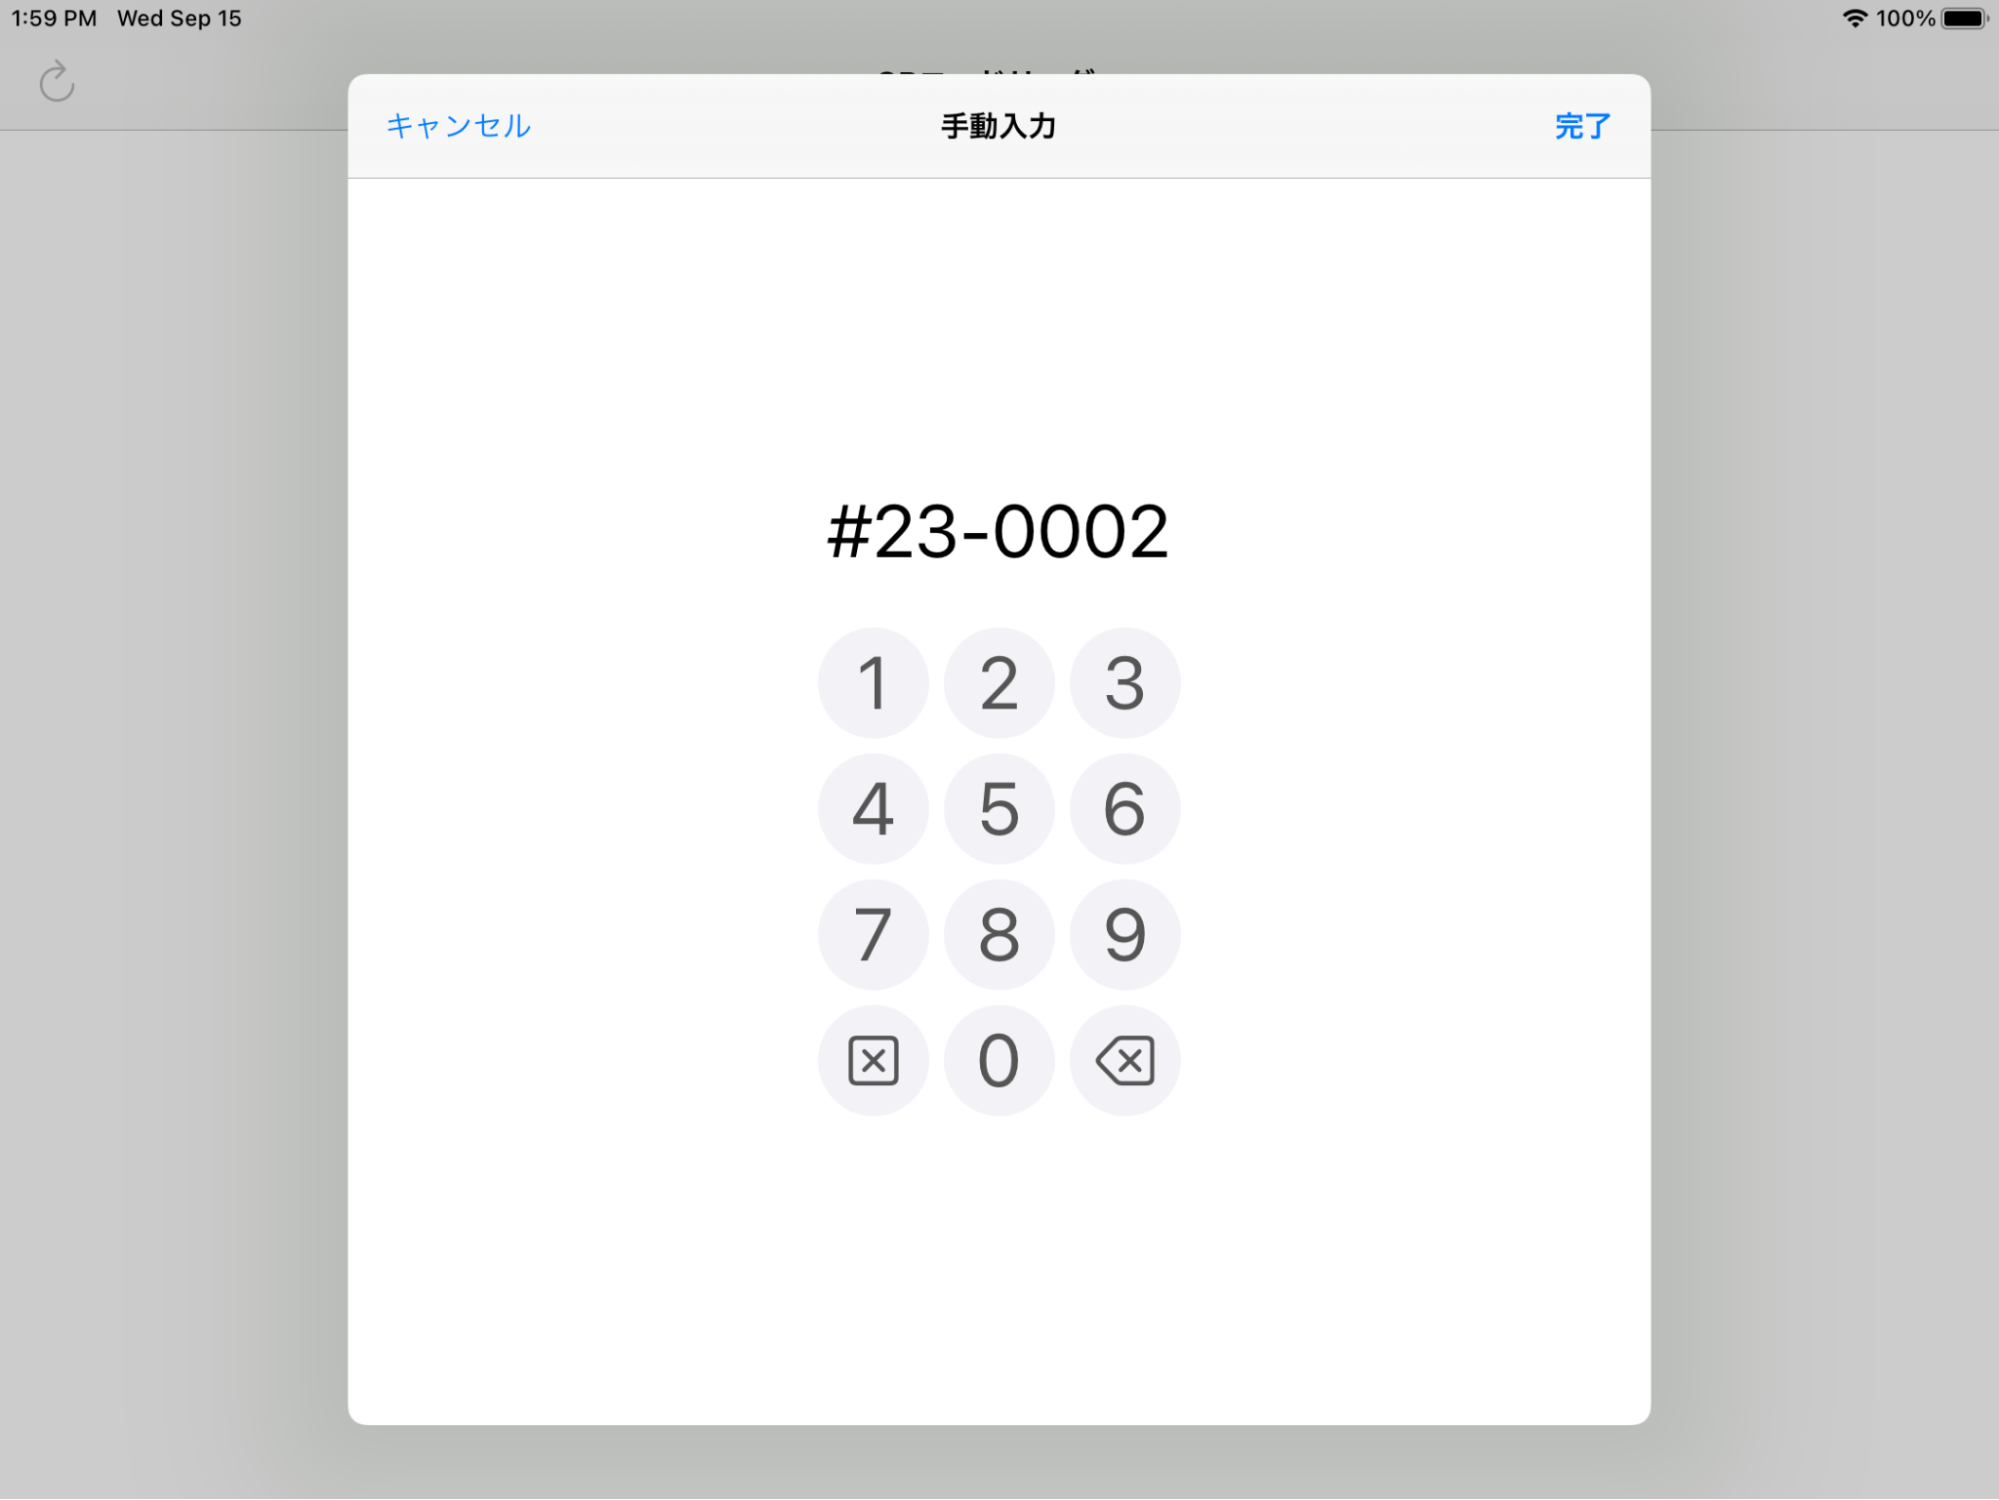
\includegraphics[scale=0.2]{assets/entrance-system-keypad.png}
  \item 表示される情報
   \begin{itemize}
    \item セイ$\cdots$代表者の姓のカタカナ表記。受付時にお客様に確認する。
    \item メールアドレス$\cdots$代表者のメールアドレス。
    \item 入場時間$\cdots$$n$日目の午前or午後。確認し、違かった場合は幹部や担当を呼ぶ。
    \item 入場区分$\cdots$一般or関係者orその他。保護者に対する特別措置がある。
    \item 人数$\cdots$グループ内の人数。実際来た人数以上だったら 3. シール印刷 に沿って印刷を行う。そうでなければ幹部や担当を呼ぶ。
   \end{itemize}
   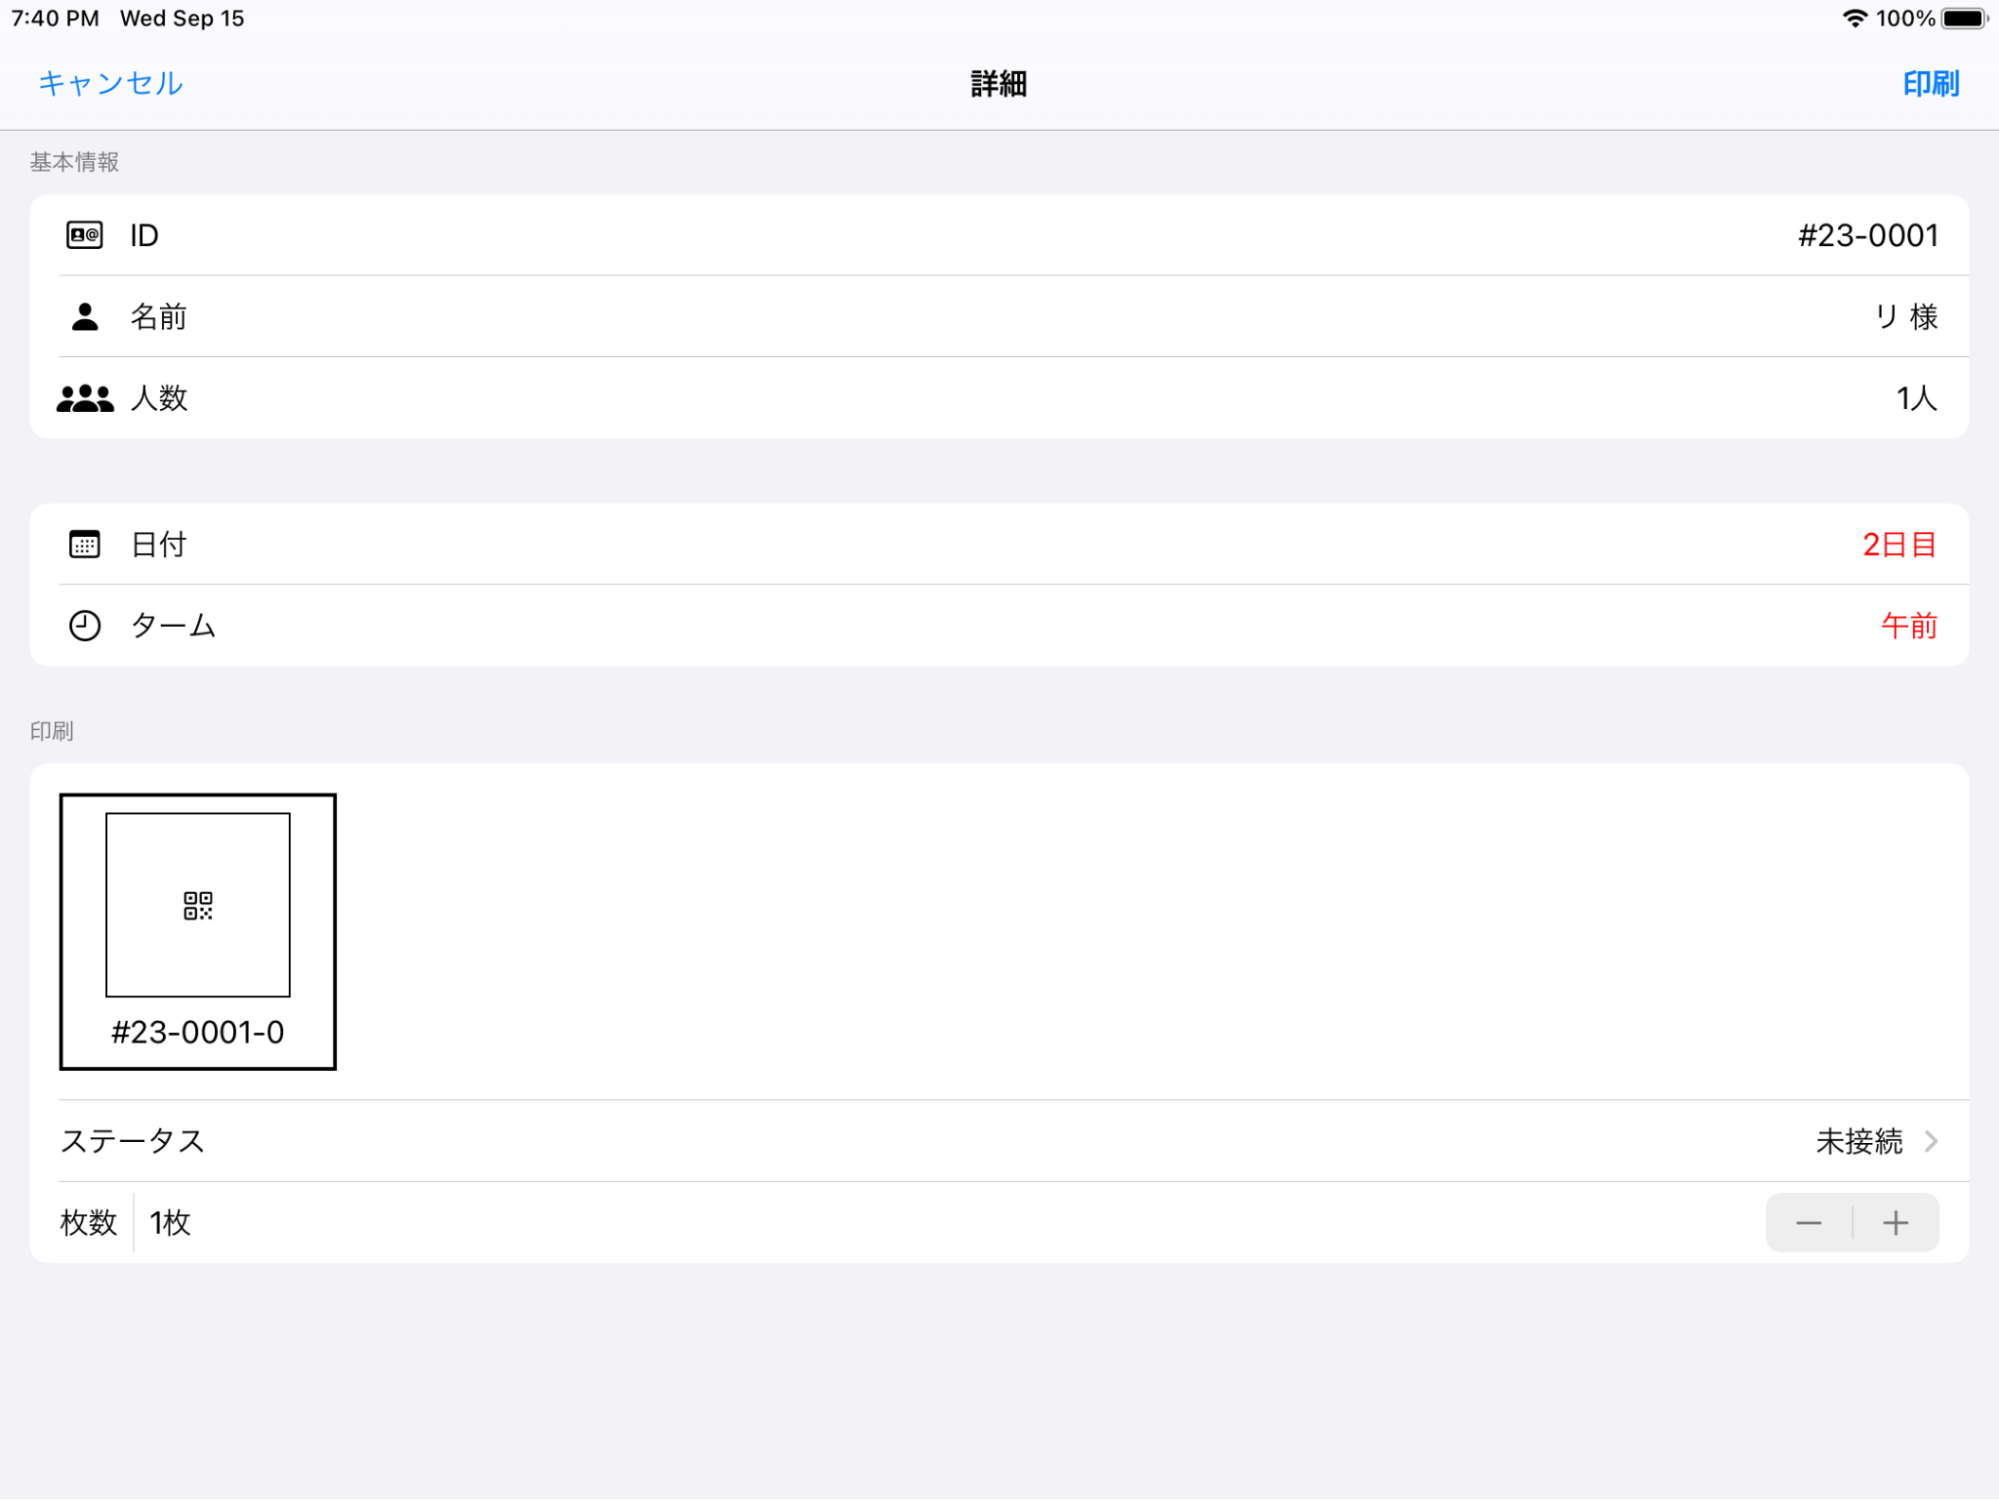
\includegraphics[scale=0.2]{assets/entrance-system.png}
 \end{enumerate}
    登録されている日付と時間帯が、現在の日付と時間帯と間違っている場合は、それぞれが赤く表示される。
 \subsubsection{シール印刷}
 本人確認後、人数を調整して印刷ボタンを押す。5~6秒まって印刷されない場合は幹部や担当を呼ぶ。1グループ分が一本のシールの束で印刷される。
\subsection{展示団体入退場管理システム}
\subsubsection{概要}
お客様一人一人にIDを配るなら各教室の入場人数を測れるのではということで実装した。入場退場の人数を記録し、現在入場中の人を算出する。
\subsubsection{必要物品}
展示団体ごとに入口と出口にChromebookを配置。Chromebookは各団体の団体員に出させる。

\subsubsection{構成}
\begin{itemize}
  \item Google Spread Sheet\\
  DB。データを格納する。ここに展示団体IDと現在入場中の人数と累計入場人数が記録されている。
   \item Google Apps Script\\
   DBからデータの抽出と数字の増減を行う。
   \item nuxt.js + scss + javascript\\
   typescriptの導入を忘れてた。
   \item jQuery\\
   Ajax通信したいので入れた。
   \item Firebase\\
   作ったWebサイトをホストするためにFirebase Hostingを使った。
  \end{itemize}

\subsubsection{仕組み}
URLのクエリで\verb|type=in|だったら入場。それ以外は退場モードになる。QRコードリーダーに個人IDを被せると通信し、入場可能か否かの結果が出る。以下は入場が許可されない事例。
\begin{itemize}
\item IDが無効な時
\item 校門で入場してから3時間が経った時
\item 展示団体の現在入場中の人数が最大収容人数を越している時
\end{itemize}

\subsubsection{入場許可}
入場許可が降りなかったとしても入場するなと強制することはできないのであくまで``遠慮していだたく''形になることに留意すること。

\subsubsection{課題}
Chromebookの性能が悪いため、QRコードの読み取りに時間がかかる。『解決策は見当たらない。』\footnote{厨病激発ボーイ - れるりりfeat.鏡音レン}

\subsection{講堂棟予約システム}
 \subsubsection{目的}
 グランドフィナーレなどの人気企画で、会場内が密になるのを避けるため、事前に座席を指定しておくことで、新型コロナウイルス感染防止を目指す。
 \subsubsection{必要物品}
 \begin{itemize}
 \item iPad(2台)... 予約アプリケーションの実行
 \item 感熱式ラベルプリンター(2台)... チケットの印刷
 \item ゴミ箱 ... 剥がしたシール台紙を捨てる用
 \end{itemize}
 \subsubsection{予約受付マニュアル}
 \begin{enumerate}
  \item QRコードをスキャン\\
  スキャン前に、QRコードが「 \#31-○○○○」の形であることを確認する。もし違う場合、担当者を呼ぶこと。\\
  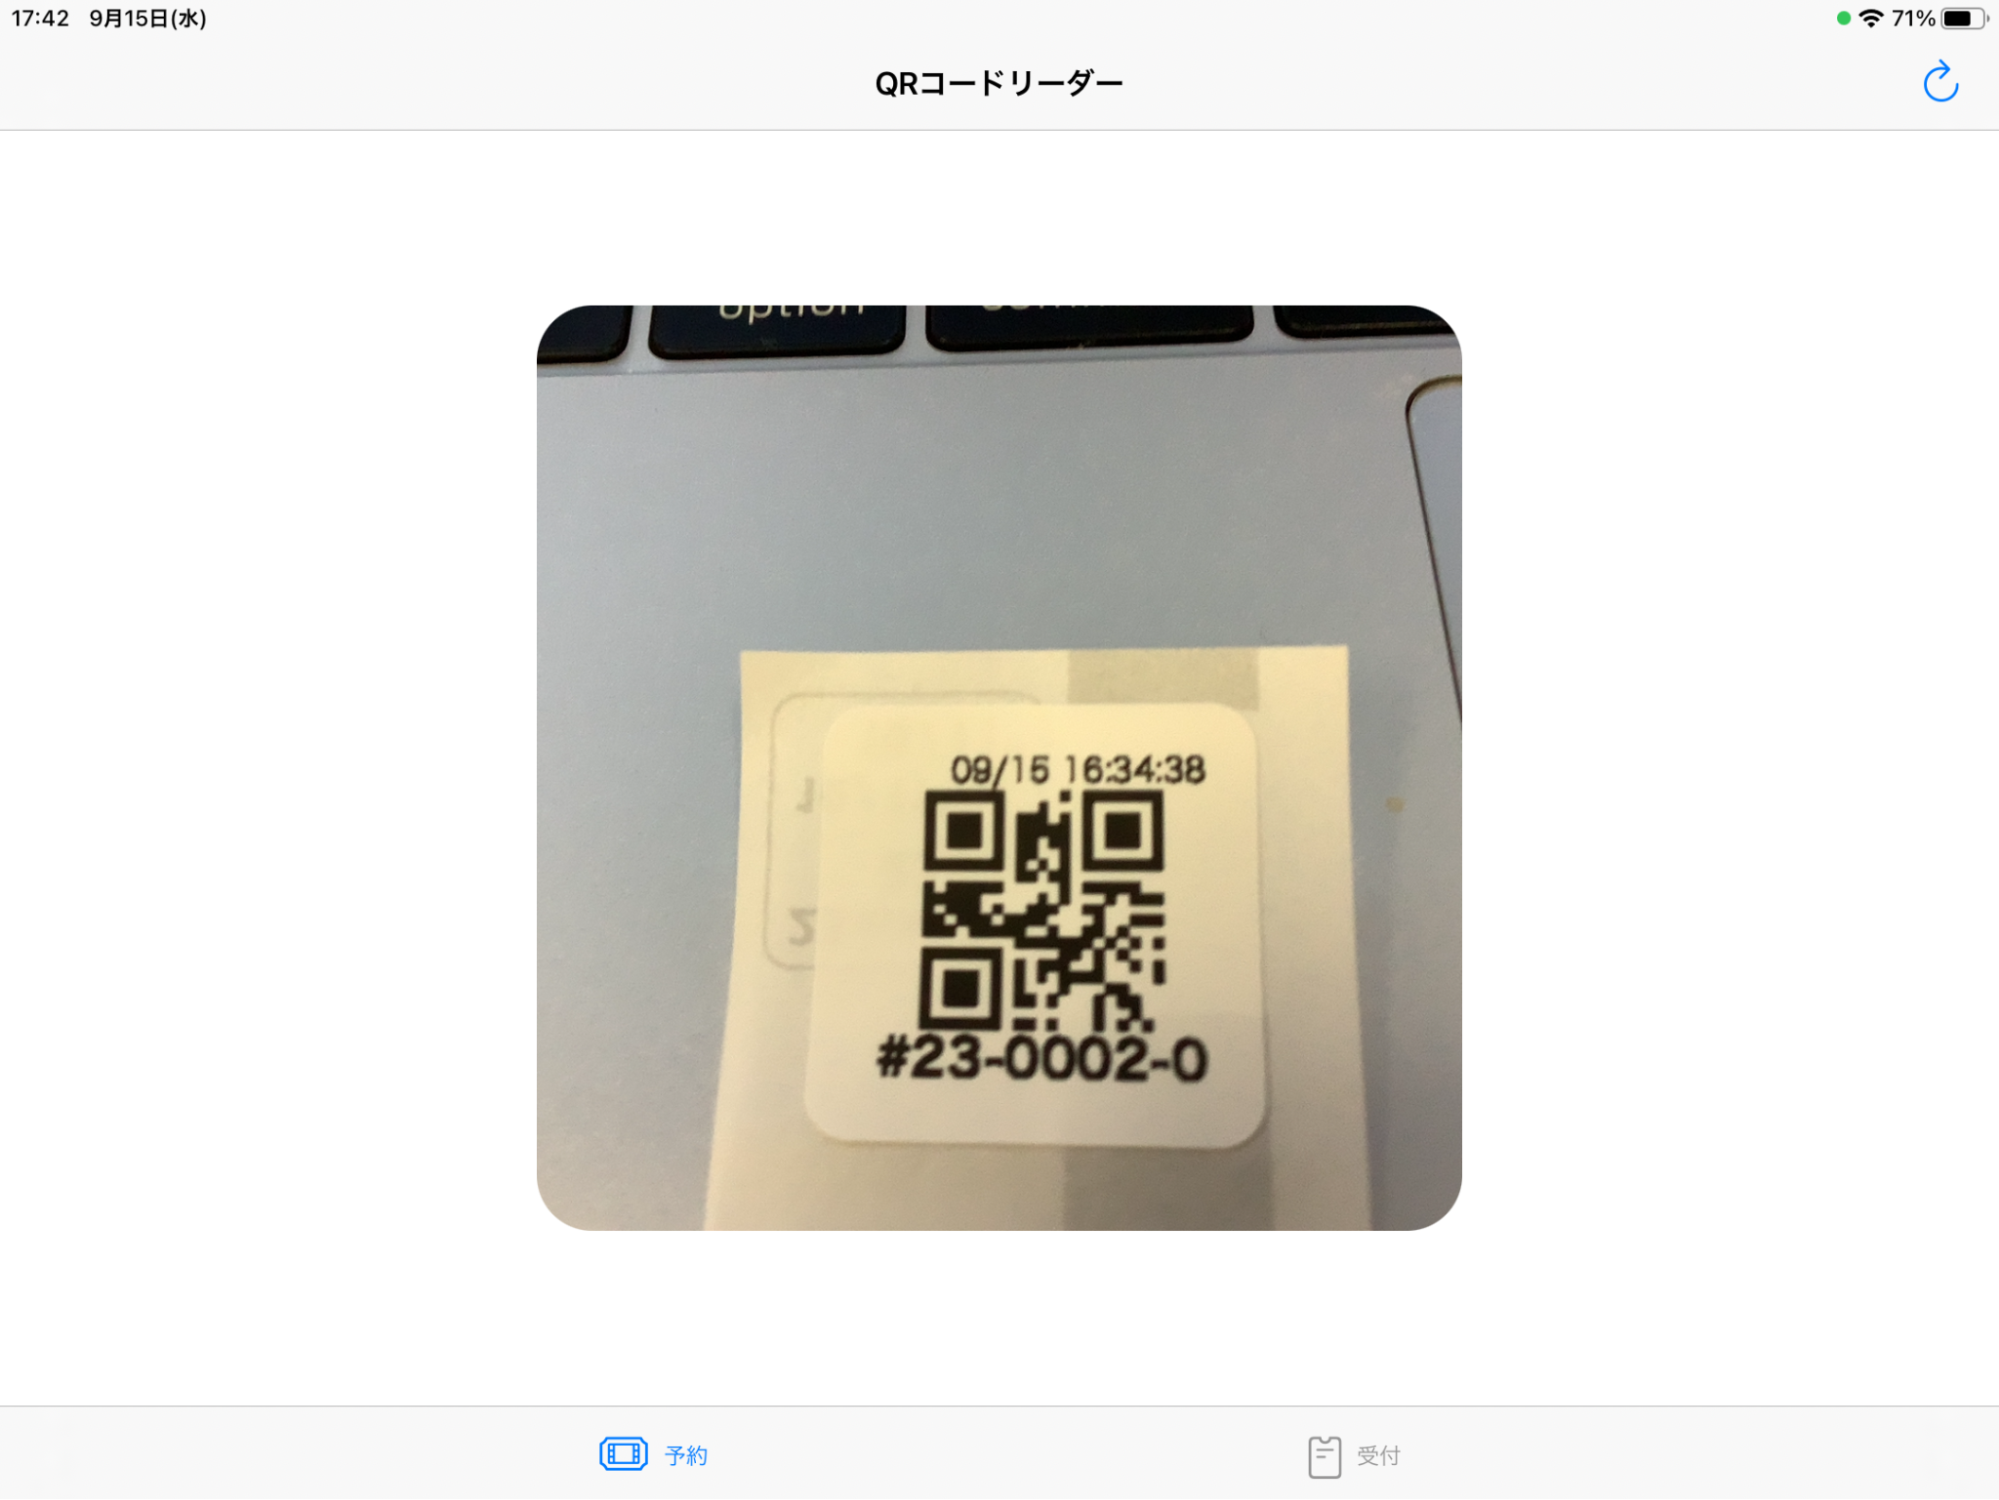
\includegraphics[scale=0.2]{assets/auditorium-seat-reservation-system_QR.png}
  \item 座席を指定\\
  座席票をお客さんに見せる。ただし、画面を操作させないこと。\\
  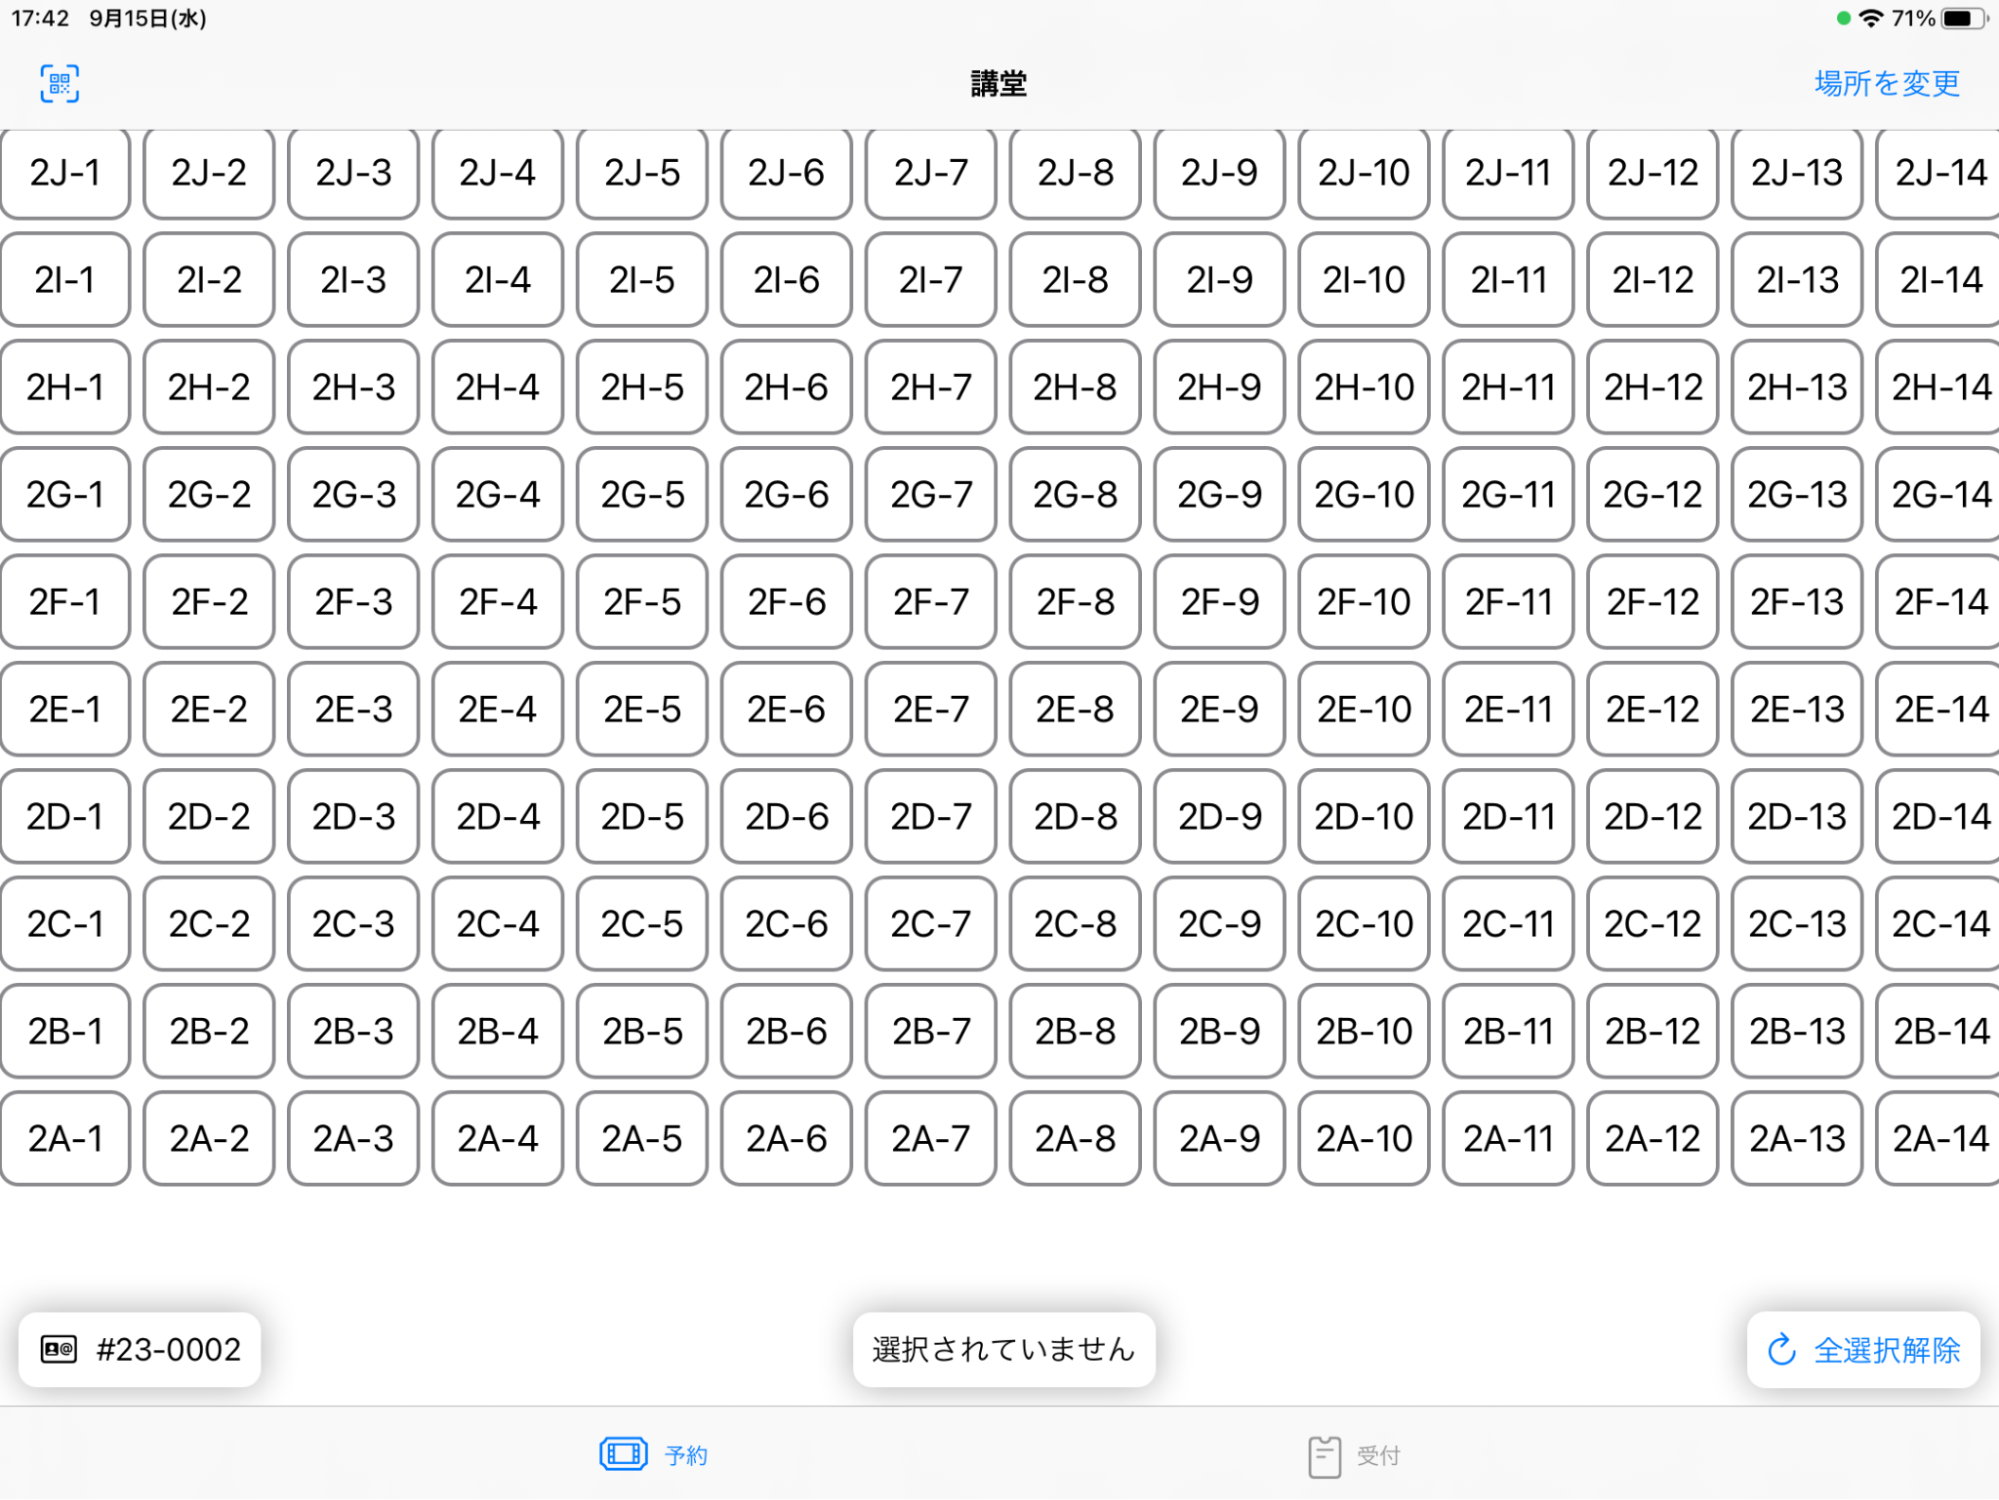
\includegraphics[scale=0.2]{assets/auditorium-seat-reservation-system_select-seat.png}\\
  元々利用できない席は紫色、既に予約されている席は赤色で表示される。また現在選択中の項目は、青色で表示される。全選択解除したい場合は右下のボタンを押す。選択完了後は確認を取ること。\\
  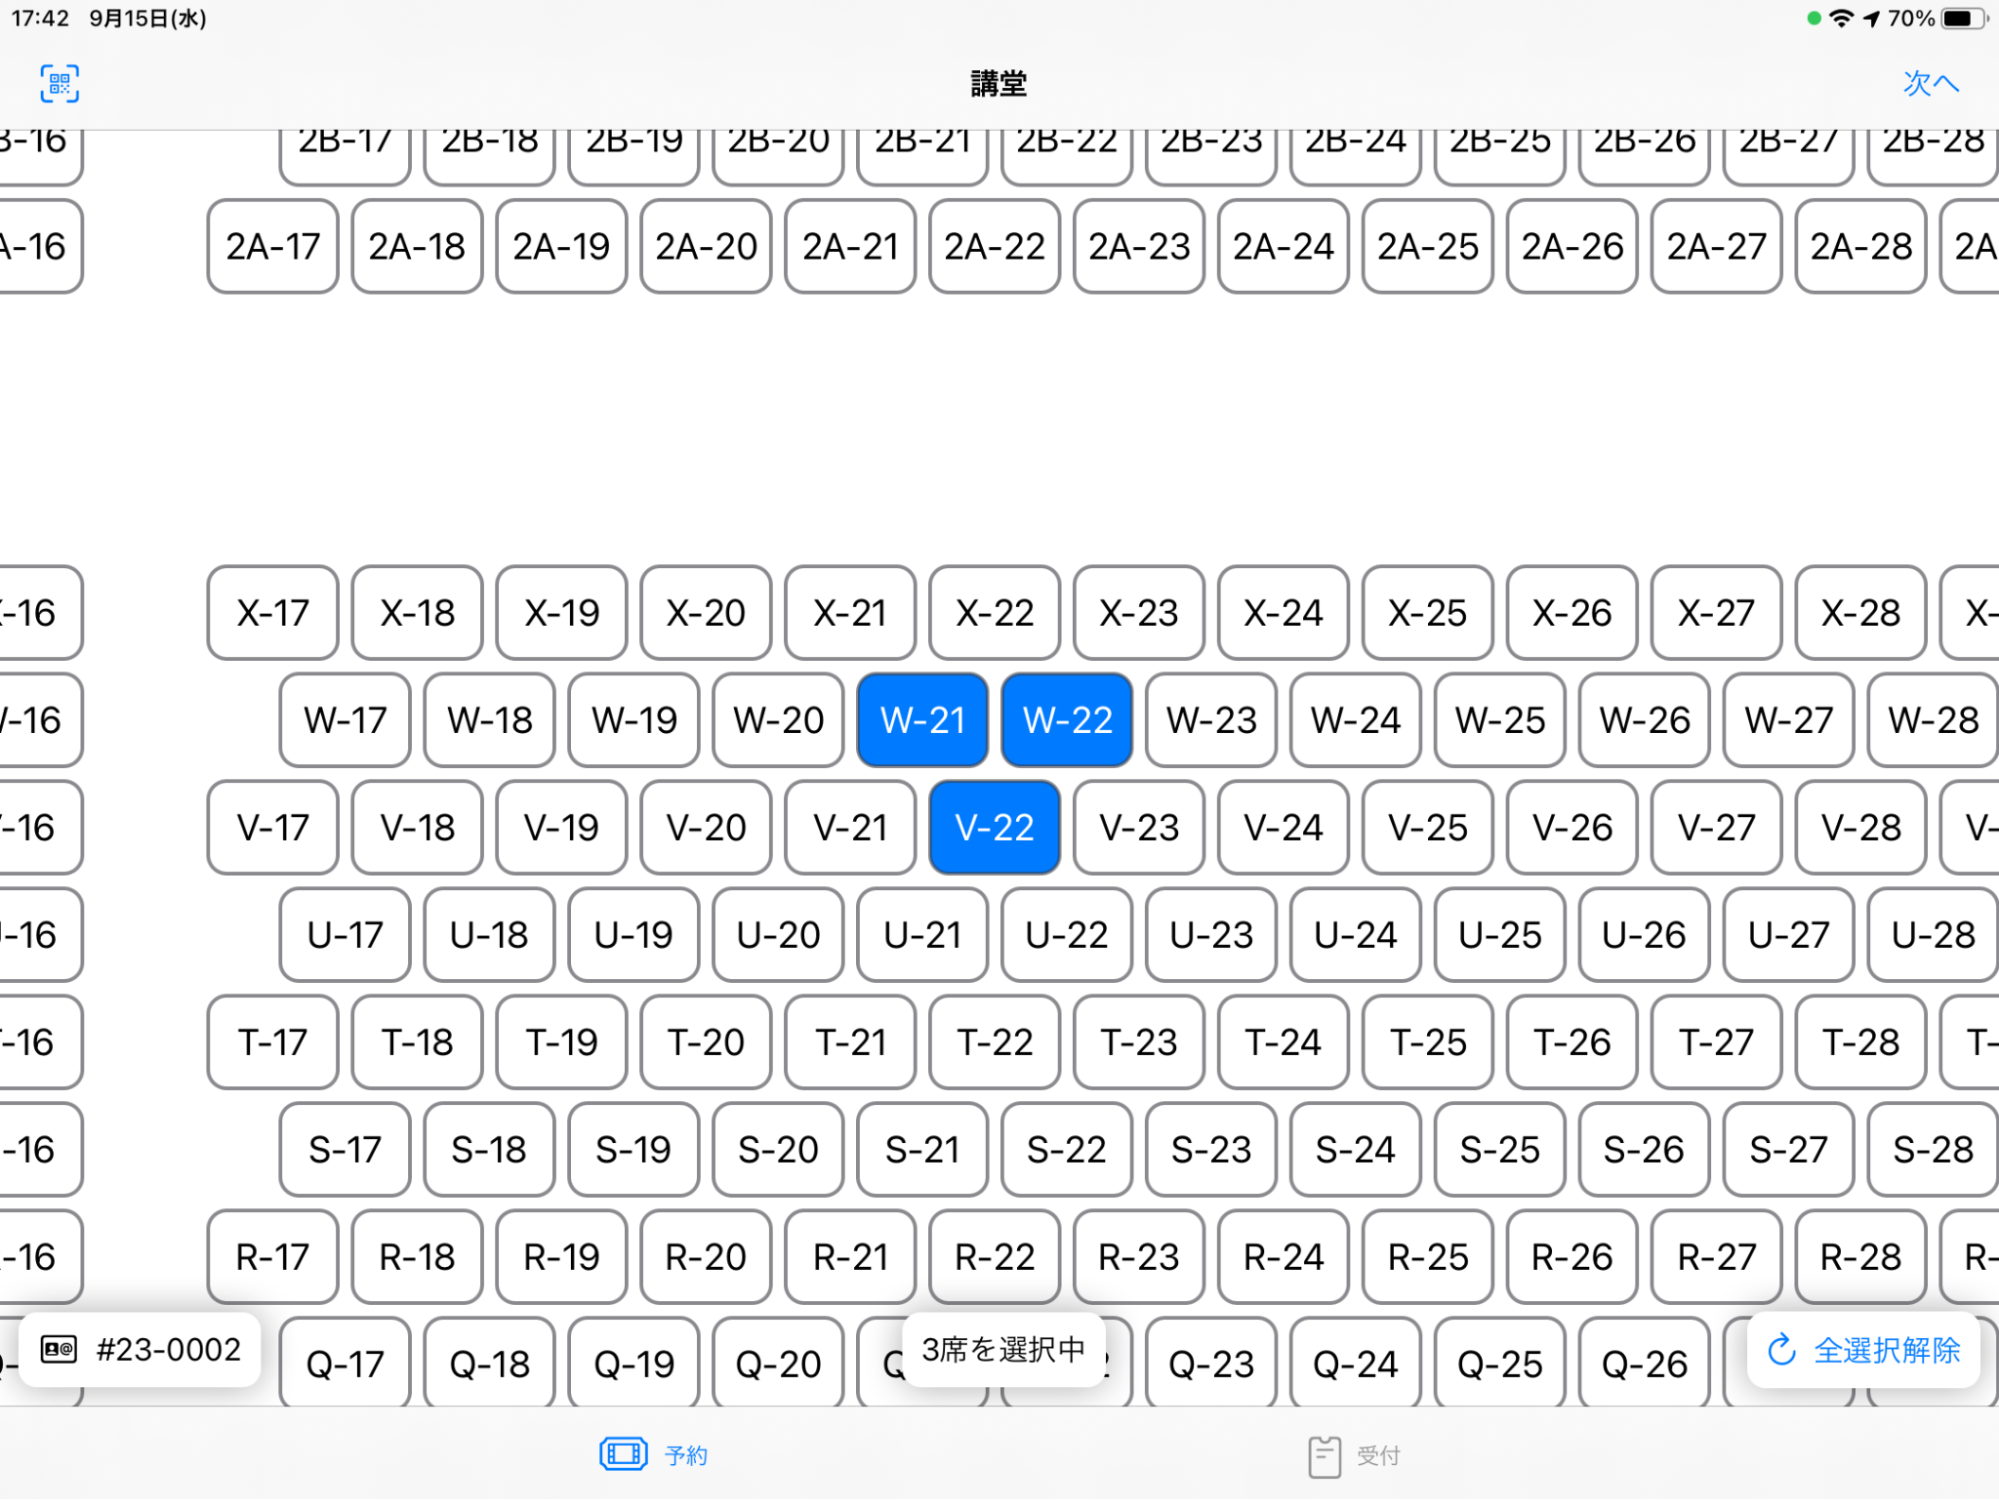
\includegraphics[scale=0.2]{assets/auditorium-seat-reservation-system_selected-seat.png}
 \item 確認・印刷\\
 名前を確認し、印刷する。印刷された入場券はお客さんに貼ってもらう。
 \end{enumerate}
 \subsubsection{入場受付マニュアル}
 \begin{enumerate}
  \item 下のタブバーで「受付」を選択
  \item QRコードリーダーが表示されるのでスキャンすると入場の可否が表示される。
  \end{enumerate}
 \subsubsection{仕組み}

 \subsection{iPad}
 \subsubsection{仕様}
  iPad(第8世代)。
  \link{詳しく見る}{https://support.apple.com/kb/SP822?viewlocale=ja_JP&locale=ja_JP}
 \subsubsection{周辺機器}
  \subsubsubsection{充電ケーブル}
  買った時に付属していたもの。1〜20の番号がついている。
  \begin{itemize}
   \item \link{20W USB-C電源アダプタ}{https://apple.co/3xeTw5G}
   \item \link{USB-C - Lightningケーブル(1 m)}{https://apple.co/3cGxn6D}
   \end{itemize}
  \subsubsubsection{ラック}
 \subsubsection{購入した経緯}
  2015年、iPad mini3が50台導入されたが、設定が不十分だったことや経年劣化により2020年には20台ほどしか使えるものが残っていなかった。iPadOS 13以降が利用できないことから2021年3月に動作するものもしないものも全て売却\footnote{Lightningケーブルなどは販売しなかった}。その後、聖光祭で使いたいと申し出たところ、破棄\footnote{当初は「破棄」と説明、のちに「売却」だと判明}されたことが判明し、新規にiPadを20台購入することとなった\footnote{購入にかかった金額の約半分は売却したiPad miniの金額で賄った}。
 \subsubsection{セットアップ}\label{sec:iPadのセットアップ}
  \subsubsubsection{Apple Configurator2}
   セットアップに必須なアプリケーション。Mac専用。\\
   かなりマニアックなアプリである。\\
   \url{https://apps.apple.com/jp/app/apple-configurator-2/id1037126344?mt=12}
  \subsubsubsection{Wi-Fi}
  生徒会のiPadやMacで設定されているstudentを使用してもいいが、回線速度や使えない時間帯があるという観点から、projectorC(5GHz)やprojectorE(2.4GHz)といったWi-Fiを使うようにした方が良い。\\
  こういったWi-Fiを登録するには、Wi-Fiのパスワードが必要なわけだが、もちろん学校側はパスワードを教えたくないし、iPad20台全部に入力するのもめんどくさいので、こう言った時にプロファイルを使う。プロファイルの作り方は\ref{sec:プロファイルの作り方}、インストールの仕方は\ref{sec:プロファイルのインストール}参照。\\
  また、studentのWi-FiやprojectorEは自動接続をオフに設定しておくことを推奨する。
  \subsubsubsection{プロファイルの作り方}\label{sec:プロファイルの作り方}
  \begin{enumerate}[手順1.]
   \item Apple Configurator2を起動
   \item メニューバーからファイル>新規プロファイルをクリック
   \item プロファイルの名前、組織名(推奨)、説明(任意)、同意メッセージ(任意)を入力
   \item 設定したい項目を選んで設定を入力
   \item メニューバーからファイル>保存より保存先を選択し保存。
   \item 保存先にあるファイル\footnote{拡張子は\texttt{.mobileconfig}}が完成したプロファイル。
  \end{enumerate}
  \begin{itembox}[l]{【注意】}
  一回設定を保存すると、プロファイルを作ったMac以外ではそのプロファイルが編集できない。\\また、Wi-Fiなどのパスワード類は一度Macに入力すると、保存する前ですら、何が入力されたか表示することはできない。\\正しいパスワードが入力されているかどうかは、実際に端末にインストールしてみないとわからない。
  \end{itembox}
  \subsubsubsection{プロファイルのインストール}\label{sec:プロファイルのインストール}
   \begin{enumerate}[手順1.]
    \item Apple Configurator2を起動
    \item セットアップするiPadをMacに接続
    \item 「追加」からプロファイルを選択しインストール。
  \end{enumerate}

  \subsubsubsection{Apple School Manager}
  学校用のApple IDを管理するもの。\\
  聖光学院では2021年7月にiPadを購入した際に学校用Apple IDを取得した。\\
  Apple School Managerを使えば、Appの購入と割り当てができる。
  Apple School Managerにログインするためには、\impact{教師アカウントが必要}なので、
  \url{school.apple.com}からアクセス可能。
  \subsubsubsection{Apple ID}
  iPadのApple IDはできれば全デバイスでバラバラの方がいい。\\
  第62回聖光祭では他のiPadから別のiPadへのアクセスを防止するという理由で、別々のApple IDでログインしていたが、アクセスガイドを使って、ほとんどのiPadで一つのアプリケーションしか使えないようにする設定をしていたため、意味がなかった。いたずら防止のため、電子決済用のiPad間だけでは別々のApple IDを設定しよう。
  \subsubsubsection{Appの購入}
  Appのインストールの前に、ライセンスの購入を行う必要がある。\\
  \begin{enumerate}[手順1.]
   \item Apple School Managerにサインイン
   \item 「コンテンツ」セクションの「Appとブック」からアプリを選択
   \item ロケーションで「聖光学院中学校高等学校」を選択
   \item 必要な数量を入力
   \item 入手を押す
  \end{enumerate}
  \subsubsubsection{Appのインストール(割り当て)}
  Apple School Managerから十分なライセンスがあることを確認すること。
  \begin{enumerate}[手順1.]
   \item Apple Configurator2を起動する。
   \item (初めての場合)メニューバーからアカウント>サインインから教師用アカウントでサインイン、Select Locationで「聖光学院中学校高等学校」を選択。
   \item iPadを接続する。
   \item iPadを選択して、「追加」からAppを選択して追加する。
  \end{enumerate}
  \subsubsubsection{TestFlight}
  オリジナルAppをiPadに入れるためには、TestFlight Appが必要。このアプリは本来、アプリのベータ版を配信するときに使われるものだが、iPadで利用するのには\impact{教員用Apple IDでApp Storeにログインする必要がある}\footnote{デバイスの「設定」AppでログインしているApple IDとは別。iPadセットアップ時にログインするApple IDと同じデフォルトで設定されている。App Store App上でそのApple IDからログアウトしてサインインしなおせば、デバイスのApple IDとは別のApple IDでログインできる。}\\
  TestFlightへのアップロードに関しては\ref{sec:TestFlight}参照。
  \subsubsubsection{アクセスガイド}
  iPadにある1つのAppしか使えないように制限するモードである。\\
  電子決済をしない全てのiPadで設定すべきである。
  \begin{enumerate}
   \item アクセスガイドを設定する
   \begin{enumerate}[手順1.]
    \item 「設定」>「アクセシビリティ」の順に選択し、「アクセスガイド」をオンにする。
    \item 「パスコード設定」をタップし、「アクセスガイドのパスコードを設定」をタップする。
    \item パスコードを入力し、もう一度入力する。
   \end{enumerate}
   \item アクセスガイドのセッションを開始する
   \begin{enumerate}[手順1.]
    \item 固定したいAppを開きす。
    \item ホームボタンを 3 回押する。
    \item 画面の一部がタッチ操作に反応しないようにする場合は、1 本指を使って、その部分を円で囲みす。円は移動したりサイズを変更したりできす。また、「$\times$」をタップして削除できす。
    \item 「アクセスガイド」をタップし、「開始」をタップする。
   \end{enumerate}
   \begin{itembox}[l]{【利用できるようにする機能をコントロールする】}
    機能を無効にしたり時間制限を設けたりするには、サイドボタンまたはホームボタンを 3 回押して、「オプション」をタップする。
    \begin{center}
    \begin{tabular}{|c|l|}\hline
     スリープ/スリープ解除ボタン&スリープ/スリープ解除ボタンを無効にする\\ \hline
     ボリュームボタン&デバイスの音量調節ボタンを無効にするには\\ \hline
     動作&デバイスが動きに反応しないように制限する\footnote{シェイクしても画面が反応しなくなり、デバイスの持ち方を変えても画面が回転しなくなる}\\ \hline
     キーボード&キーボードを無効にして表示されないようにする\\ \hline
     タッチ&画面をタッチしてもデバイスが反応しないようにする\\ \hline
     辞書検索&テキストを選択したときに「調べる」機能を無効にする\\ \hline
    \end{tabular}
    \end{center}
   \end{itembox}
   \item アクセスガイドのセッションを終了する
   サイドボタンまたはホームボタンを 3 回押して、アクセスガイドのパスコードを入力してから、「終了」をタップする。
  \end{enumerate}

  \subsubsubsection{Apple Classroom}
  Apple Classroomを使えば、Wi-Fi経由でリアルタイムでiPadを監視したり、ロックできる。ただし同じWi-Fiに接続されていることが必要。
  \begin{enumerate}[手順1.]
   \item 管理するMacまたはiPadに\link{クラスルーム}{https://apple.co/3DShnKU}をインストールして開く。
   \item 「教師の情報」に名前を入力して写真を追加する。
   \item +を選択して新しいクラスを作成し、クラスに名前を付け、クラスのカラーとシンボルを選択する。
   \item 「生徒に参加を依頼」を選択して、生徒を招待できるようにする。
   \item 生徒として追加するiPadで「設定」を開く
   \item 左のメニューに「クラスルーム」が表示されるので\footnote{表示されない場合は、同じWi-Fiに接続されているか確認すること}、「<クラス名>を追加」を選択して、生徒の情報と、管理する端末に表示されている確認コードを入力する。
   \item 「追加」を選択すると、設定が完了し、管理する端末に生徒の情報が表示される。
   \item 「教師に許可する操作」の「Appとデバイスのロック」「AirPlay及び画面の閲覧」を「常に」設定。
   \item それぞれのiPadで以上を繰り返す。
   \item 管理する端末で「追加」を選択して、クラスルームに生徒が追加された。
  \end{enumerate}

\subsection{外務送付状の差込}\label{sec:外務送付状の差込}
62回担当:飼沼

\href{https://script.google.com/d/1peO_Bmf9jcnJWGCZMN2IRhBrCqokkgPmUVuC4BlryH9kxAiHoXzkjO_x/edit?usp=sharing}{スクリプト}を組んで外務部門が企業や学校に送るポスターの送付状を差し込みした。リストをスプレッドシートでもらって雛形の学校名とかの部分を変えればいい。

\begin{lstlisting}
let cnt = 0

const folder = DriveApp.getFolderById("12DpG8U-czSkeJgyYXRdoinP6V2yVLUxG");

function main() {
  var iterList = folder.getFiles();
  while (iterList.hasNext()) {
    iterList.next().setTrashed(true);
  }
  createNewDocument("1OGJbc8RwnVNB_fq_yPwDh0i7W7kZjsT21KKE-yRjYyw", "K1:K93", "12cfVYAmyq8II-733FvNCqhpCs32OV5g4TQ3qGDZ7jS8");
  createNewDocument("1XY8ZKv1cQ6vfYcZjxhmSHoJosh3_zW3d2s8aK6Kc3wA", "B2:B60", "1r25jPkAtN8ukkBs7bjL82eWLgRuIzJ2ymWfiM7AiSSQ");
}

function createNewDocument(id, range, sdid) {
  const values = SpreadsheetApp.openById(id).getSheetByName("シート1").getRange(range).getValues();
  const sourceDocument = DriveApp.getFileById(sdid);

  for (array of values) {
    cnt++;

    const name = array[0];
    const duplicateDocument = sourceDocument.makeCopy(name, folder);
    const ddId = duplicateDocument.getId();
    const targetDocument = DocumentApp.openById(ddId);
    const targetBody = targetDocument.getBody();

    targetBody.replaceText("\\[name\\]", name);
    targetDocument.saveAndClose();
    Logger.log(cnt);
    Utilities.sleep(2000);
  }
}
\end{lstlisting}

\section{体育祭}
\subsection{名簿管理}
\subsection{Tシャツ}
\subsection{装飾物デザイン}
\subsection{オンライン得点板}
36回担当:李\\

スプレッドシートの値を持ってきてサイトに表示すれば良い。2日で実装できるのでそんな大変ではないはず。コロナによって2日間開催になった時に来ていない学年や保護者に向けた措置。あって困るものではない。スプレッドシートは記録課が作るのでそれに合わせて作る。初心者にやらせるとかなりいい勉強になる良教材。実装できないとなることはないだろう。
\subsection{撮影}
広報委員会で撮影隊が結成されていないのであれば、動画局が代わりに撮影スタッフを募集すること。撮影と言っても写真がメインで良い。
\subsection{動画局}
ダンス動画の編集をしろみたいな流れがあったが、編集は頼まれた時のみやればいいと思う。
\section{生徒会}
\subsection{Across}
58期の代は洗足学園など他校の生徒会とともに学生団体「Across」が結成されていた。ただ、59に引き継がれた後パンデミックの間に有耶無耶に。僕(飼沼)はAcross Business Plan Contest 特別講演会ポスターの代金を踏み倒されているので、経理が判明したら連絡をください。

\subsection{生徒総会・生徒集会}
\subsection{撮影}
活動風景は積極的に撮影すべきです。拡大役員(副委員長・委員等込み)の集合写真も撮ろう。

\subsection{食堂}
58期の代から食堂改革は行われています。僕(飼沼)はこの代のインフォグラフィック責任者でした。食堂の列整理などを行う際は、食堂の方に必ず挨拶した上で、生徒会での希望があることを伝えよう。なかなか対応してくれることは少ないと思います。なお、食堂・購買に導入するとして交渉した電子マネー企業は、聖光祭のものと異なる会社です。

\subsection{目安箱}
生徒会Slackにフォームの回答を投下し議論できるようにしていた。
\subsection{広報}
\subsection{一般IT環境}
\subsection{生徒会室}
\subsubsection{清掃}
たまに中のものを全て出して掃除しよう。汚すぎ
\subsubsection{鍵}
生徒会長と事務局長のみ持ち出し権限がある。聖光祭中は実行委員長と副実行1が権限持ちだった。早く来すぎて開けれないとかはよくあったので、生徒会長に相談するといいと思う。紛失するなよ絶対。
\subsubsection{PC}
事務局PCと技術局PCがある。生徒会長/事務局長/技術局長以外使用禁止にしよう。それ以外の人が使うときは許可もらってからがいいと思う。
\subsubsection{その他}
備品勝手に持ち出すべからず。たまに換気すべし。天窓を開けて侵入できるようにしておくべし。高3に迷惑をかける&空調が妨害されるので扉はすぐ閉めるべし(ただし換気中(ただし事務局印刷機を稼働中を除く。)を除く。)。\footnote{今年は「ドアベリング(ドア+トラベリング)」制度があった。扉を開けてから3歩以上歩くと反則が1点適用される。5点貯まると生徒会室にしばらく出入禁止になる。}
\subsection{規則}
教員たちは「生徒会の生徒会化」が嫌いです。つまり、役員の方から自治的(ルールに則った公正な)方法を提案しても、教員は役員と一緒に穏便に済ませようとしてきます。そもそも教員がなんでこんなに予算とか選挙とかに口出してくるかというはなし\footnote{理由1:聖光の生徒会が未熟だから。そもそも生徒に自治意識がなく、ほとんどの生徒はそれがどうかしたか?状態なので選挙以外で生徒会に対する決定に関わろうとしません。パンデミック以前には予算審議を生徒総会で行い拍手\footnote{起立にしろよ}多数の賛成を得ていたのがなくなっても誰も何も言いません。麻布などのように自治組織が自治を行う環境ではないのです。賛否両論あるかと思いますがきちんとやるべきところをきちんとやってくれる生徒会であるべきだと僕(飼沼)は考えています。} \footnote{理由2:生徒が未熟だから。一部の役員は虚偽の噂を根拠として、一定数の生徒から想像を絶するほどの誹謗中傷を受けます。教員が最終的な砦である必要があるのは間違い無いです。} ですが、生徒会として健全な方法はそういった部分を公正に行えることかと思います。こういった所謂進学校で生徒手帳に載っているレベルの会則しか無いのは未熟だと思います。教員の言うことを真に受けず、自分で考えて行動してみてください。
\subsubsection{生徒会則}
石渡先生に「君たちの代が終わって経験したことを書いて次の代に引き継ぐ方がいい」と言われたので拒否されたら言質をとったことを言ってください。
\subsubsection{聖光祭実行委員会細則}
飯岡先生に「君たちの代が終わって経験したことを書いて次の代に引き継ぐ方がいい」と言われたので拒否されたら言質をとったことを言ってください。
\subsubsection{体育祭実行委員会細則}
\subsubsection{選挙規則}
\subsubsection{議事進行規程}
\subsection{公約}
毎年選挙当選者は校長にまとまって挨拶に行く。

役員会・定例会・拡大実行・幹部会議等の定数以上の議決によっても、公約の結果は生徒総会の決定と同じようなものであるから、当選者に対して反対的に覆すことはできない(すなわち、当選者が当該公約と齟齬のある意見決定をしない限り、定数の会議議決をもってしても否決できない)。
\subsection{選挙}
35期担当:李 博之
\subsubsection{前提}
技術として書くことはない。なぜなら監査委員会幹部しか開票をできないからである。これはあなたが技術局員かつ監査幹部であるという前提でしか読むことができないものである。
\subsubsection{フォーム}
フォームには必ず説明を載せる。説明を少しでも読んでくれるようにするために、「読みましたか?」項目を設ける。2ページ目にはラジオボタンで「候補者の氏名」、「不信任」、「棄権」を選択できるようにする。以上。
\subsubsection{処理}
\begin{enumerate}
\item できたフォームを先生に共有(オーナー権限の譲渡)
\item 先生がフォームをコピーし、全校生徒に配信
\item 無効な回答を消してもらう(ex.生徒会アカウント・pアドレス・非有権者のアドレスからの回答)
\item 新しいスプレッドシートで先生が役職ごとに回答をシートにコピー(メアドはコピーしない)
\item スプレッドシートを共有してもらう
\item COUNTIFで各候補者と棄権、不信任の票数を算出
\item $(得票割合)=\frac{(得票数or不信任数)}{(全体の有効回答数) - (棄権数)}$で得票割合を算出
\item 結果の公示文書を制作しClassroomで公示
\end{enumerate}
\subsubsection{公示文章について}
今年は値を入れるだけで円グラフを作ってくれるpackageがあったので \TeX で制作した。何回見てもやっぱりミスは存在するので落ち着いて作ろう。今まではグラフしか載せてなかったが「結果」の公示なので誰が当選したか、誰が決選投票かをはっきり明記したほうがいいと個人的には思う。載せる内容は任せる。
\subsubsection{アドバイス}
今年は選挙規則があった。全ての職務は選挙規則に基づいて行った。Twitterで炎上したり非難されたりすることはあった。現に委員長はかなり心に傷を負ったと思う。それでも続けられてるのは「僕たちは何も悪いことしていない」という自負だったように思う。選挙規則にも、生徒手帳の記載にも違反していない行動がその自負を生んだ。選挙はかなり候補者やその周りにはセンシティブな事柄であり、Twitter等のSNSでもしょうもない悪ノリをする輩が現れる。それに負けずぜひ頑張ってもらいたい。
\subsection{ビジコン}
\subsection{ホームページ}
35期担当:李 博之\\
鋭意製作中。続報を待て。
\subsection{生徒会アカウント}

\subsection{Buddycomの管理}
\subsubsection{概要}
BuddycomとはIP型のトランレシーバでつまるところスマホ用のトランシーバである。アカウントを制作し、それにログインさせることで複数の端末で会話することができる。
\subsubsection{機能と用語}
\begin{itemize}
\item テナント\\
Discordでいうサーバー、Slackでいうワークスペース。テナント編集権限=管理者権限。テナント名は\verb|seiko.ac.jp|で学校ドメインと一致。
\item 階層\\
階層を作ることができる。といっても分類できるだけでこのグループごとに操作とかできない。まだ開発途中だから今後に期待。
\item ユーザ\\
個人。ユーザごとに以下の設定項目がある。これらは全て管理者しか変えられない。
\begin{itemize}
  \item ユーザID\\
  unique。半角の英字大文字、英字小文字、数字、記号。
  \item ユーザー表示名\\
  Discordで言うニックネーム。普通に本名でよい。
  \item パスワード\\
  ユーザログインの時のパスワード。管理者だったらこれでコンソールにアクセスする。今回はランダム生成したものをスプレッドシートで管理した。
  \item 組織名\\
  今回は所属してる委員会を出した。例:\verb"生徒会|聖光祭実行委員会|体育祭実行委員会"
  \item 役職名\\
  所属部門や組織、役職を組織名に対応する形で表示した。例:\verb"副監査委員長|副技術部門|副技術局長"
  \item 電話番号\\
  いらん。
  \item メールアドレス
  \item かんたんログイン\\
  後述する。基本OFF。
  \item 割り込み権限\\
  割り込み通話(後述)で割り込めるかどうか。基本OFF。
  \item マップ通話\\
  マップ通話(後述)を許可するか。基本ONでいい。
  \item 音声テキスト化\\
  文字起こし。基本ON。
  \item 翻訳\\
  翻訳。今回はONにしたがOFFが良さそう。
  \item 動態管理\\
  位置情報がわかる。バッテリーの消費がえぐいのでOFFでよかったと反省。
  \item ライブキャスト\\
  ライブキャストを利用するかどうか。基本ONでもいいとおもう。
\end{itemize}
\item ログイン\\
ログインIDとパスワードでログインできる。ログインIDは\verb|[ユーザーID]@[テナント名]|で表される。
\item グループ(チャンネル)\\
DiscordやSlackでいうチャンネル。入ってる人で通話が可能。グループごとに設定が可能。以下はグループの設定項目。グループに参加できる人を選んで設定する。また、必須設定にすることで必ず聴くようにできる。
\begin{itemize}
\item グループID\\
unique。なぜかユーザIDとは違い、全角可能。
\item グループ表示名
\item 音声データの保存\\
保存しとけ。
\item データの保存先\\
デフォルトでいいと思うがいい感じのプラグインあればそれを使うのもあり。
\item 通話自動終了 (秒)\\
60にしてたが、30でもいいと思う。
\item 通話形式\\
以下の三つから選択。
\begin{itemize}
\item 単方向通話\\
任意の一人が通話中の時、それ以外のメンバーは通話できない。
\item 双方向通話\\
任意の一人が通話中の時、それ以外のメンバーも通話できる。
\item 割り込み通話\\
任意の一人が通話中の時、それ以外のメンバーのうち、割り込み権限を持っているメンバーのみ割り込んで通話可能。検証してない上、公式リファレンスの説明が曖昧なのでよくわからないが多分この認識であってる。
\end{itemize}
\item かんたんログイン\\
後述する。基本OFF。
\item 低ビットレートモード\\
音質下げて転送量を下げる。お借りしたアカウントは転送量の制限がないので基本OFF。
\item 位置情報\\
メンバーの位置情報を把握できる。
\item マップ通話\\
マップ通話(後述)を許可するか。基本ONでいい。
\item 音声テキスト化\\
文字起こしエンジンを選べる。オートがいいが、日本語はAmiVoiceに自動で割り振られる。今回は\verb|Google Speech To Text|を選択した。正直なんでもいい。
\item 翻訳\\
DeepL一択。DeepLしか勝たん。
\item ライブキャスト\\
ライブキャストを利用するかどうか。基本ONでもいいとおもう。
\item ライブキャストの保存
\item ライブキャスト自動終了 (秒)
\end{itemize}
\item P2P(電話)\\
個人通話。相手には個人通話で話されてると言うことがわからないので「個人通話です」とはじめに言うように指導した。メンバ一覧からP2Pできる。
\item CHAT(チャット)\\
会話の履歴をLINE風に見ることができる。会話の再生も可能。また、直接文章を送信することも可能で、読み上げられる。
\item LIVE(ライブ)\\
リアルタイムでカメラを使用して映像共有ができる。いろんな使い方がある。
\item MAP(マップ)\\
メンバーの位置情報を表示できる。また、枠内にいる人とだけ会話とかができる。
\end{itemize}

\subsubsection{管理関係}
\subsubsubsection{管理画面}
\url{https://console.buddycom.net/static/pc/login.html#/} からテナント管理権限があるアカウントもしくは階層編集権限があるアカウントでログイン。あとは直感的にわかるはず。気をつけてほしいのは以下の点。

\begin{itemize}
\item ダブルクリックは効かない。
\item ドラッグ\&ドロップが使えない。
\item セッションを維持できる時間が短い。
\end{itemize}

\subsubsubsection{権限管理}
権限管理タブで設定可能。テナント管理者を設定できる。また、ユーザの機能制限もできる。これはブラックリストみたいなもので「こいつだけライブ禁止」と言う感じで設定できる。今回は使わなかった。

\subsubsubsection{キー管理}
プラグイン。Slackと連携ができるらしい。今回は使っていない。

{デフォルト設定}
ユーザのアプリの設定を固定したり、デフォルト設定を設定できる。主にPTT\footnote{Push-to-Talk。ボタンを押してる間だけ話せる。}に強制するためのものである。これについては後述する。


\subsubsection{CSVによる一括操作について}
50人以上のアカウントを手動で追加したり、手動でグループに追加するのは面倒なので当局が提供しているcsvインポート機能を使うことである程度時短できる。スプレッドシートで処理したものcsvでダウンロードし、インポートするだけ終わる。詳しくは\verb|ユーザ&グループ > CSVをインポートする > ダウンロード|からマニュアルをダウンロードできる。``技術""部門なのに手動なんですか〜〜〜?

\subsubsection{アーカイブ}
アーカイブをすることを推奨する。管理コンソールのトーク履歴からチャンネルごとの
\begin{itemize}
 \item 通話開始日時
 \item 通話時間(秒)
 \item 発話者
 \item 種別(音声orテキスト)
 \item 通話内容(文字起こしされたテキスト)
\end{itemize}
の情報csv形式でダウンロードできるので、全体連絡と緊急連絡のアーカイブはしておくといい。ただし\impact{直近24時間のデータしか残らない}ので、毎日定時のアーカイブが必要。

\subsubsection{だれかが話し続けてしまう現象について}
Buddycomでは誰かがボタンを押してしまい、単方向通話で誰も会話できないという現象(以下、本現象という)がかなり頻繁に起きる。なお、本現象では「意図的ではない」場合にのみかぎって説明することにする。
\subsubsubsection{原因}
主に本現象はiOS版に多い。理由としては外部ボタンによる音楽の再生トリガーである。iOSでバッググラウンドサウンドを再生するにはAppleの再生機能を使うほかない。全ての再生はiOSの管理下に置かれるため、画面に一時停止/再生ボタンが表示されてしまう。buddycomはこの再生ボタンをトグルトリガーにしている。つまり、一時停止/再生ボタンを押すとPTTに設定しても勝手にトグル式の通信が開始されてしまうのである。
\par
つまるところ、以下の三つのジェスチャーリスナーが干渉しているのが原因。
\begin{itemize}
\item 外部ボタン長押しによるPTT(Buddycom)
\item 外部ボタンによる音楽の一時停止/再生(iOS)
\item 長押しによるSiriの起動(iOS)
\end{itemize}
ただし、一部のワイアレスイヤホンマイクや、適度な長押しによって反応する時もあるので一概にできないとは言えない。また、一部のAndroid端末でも同様の現象が報告されている。
\subsubsubsection{対策}
デフォルト設定でPTT式に強制しなるべく事故らないようにする。そして、最大通話時間を短くする。あとは周知させるだけ。また、緊急連絡グループを必須設定にし、本現象が怒った際にはここで対応する。これ以上は何もできない。

 \section{さいごに}
 \subsection{精神的な話}
 \subsection{ひとこと}
 \subsubsection{李より}
 ここまで読んでくれてありがとうございます。せっかくこんなに書いたので最後に少し自分語りときしょい駄文を連ねたいと思います。
 \\

 情報技術統括所において文字通り``必須である仕事''は存在しません。これを読んだ人は聖光祭を、生徒会を、あるいは体育祭を、よくしようと思っているのかもしれませんが---もちろんそれ自体はかなり重要な話ですが---情報技術統括所で生徒会や聖光祭を作ることはできません。よく考えてみてください。技術部門がない時代、情報技術統括所がない時代に生徒会や聖光祭がなかったわけではないのです。
 \\

 貴方たちは---そして私たちの一部は---自分達が聖光祭を作っているという迷信にしがみつき、自らの仕事自体に価値を見出しています。はっきり言いますが僕がやったこと、そしてこの団体がやってきた全ての活動は``必要ない''ものです。ですが、``意味のない''ものではありません。私たちの仕事は聖光祭に、生徒会に、そして体育祭に付加価値をつけることであり、それを自らが享受することです。
 \\

 結局は自己満足のための活動なのです。自分達が何を作りたいか、やってみたいか。それが結果として行事や生徒会を良くしていくのです。同様に雑用係でもありません。仕事はあなたたちがやりたいことをやりましょう。あなたたちの身勝手でいいのです。
  \\
  
  今回の聖光祭で私は多くのことをやりました。でもそれは誰のためでもなく自分の人生経験のためです。迷惑をかけたのも怒らせたのも呆れられたのも嫉妬されたのも非難されたのもすべて自分のエゴによって作り出された結果です。開き直っているように聞こえますが、それがノルマが存在しない自己満足と承認欲求にまみれたこの情報技術統括所の実態だと思います。
  \\
  
 貴方たちのすべきことは模倣ではなくわたしたちを否定し、常に``既存''を壊して作りだすことです。作り出したものが同じであれ、それは貴方たちの選択の結果であり、貴方たちの経験というまた違う意味を持つでしょう。
 \\
 
 さて、ではなぜこの引継書を作ったのか。それは``こうゆうのが書きたかった''のと、``多分一生見向きもされないことを残したかった''のだと思います。わかりませんか?本書は\TeX で作られた。そうゆうことです。
 \\
 
 最後の``会社ごっこ''に付き合っていただきありがとうございました。それではまた。
\subsubsection{飼沼より}
ゴミみたいに長い引継書をごめんなさい。しかも未完で。
\\

技術部門の仕事は必要なものではありません。聖光祭の延期会議では技術幹部は「技術部門のことを考えないで議論を行う」ようにお願いしました。技術部門の幹部だからといって、自分が何かに秀でているからといって、その技術力を他の幹部や生徒を黙らせるために使うのは言語道断です。別に仕事をしているから偉いなんてことはないのです。自分の部門の仕事だけやっていて周りが見えなくなっていたら尚更です。
\\

卑屈になれというわけではありません。どうしたいかを考えてやってください。そういう意味では、この引継書は今年僕らが何をしたかという参考資料として以外の意味を持ちません。君たちが生徒会を、聖光祭を、体育祭をどうするかの可能性は無限です。
\\

多分色々としっかりとやれるのは早いうちだけです。当日に近づくにつれ、最初に議論して放置していた内容とか、予算とか、全部どうでも良くなって来ます。最後はがむしゃらにやる他間に合わないです。
\\

ただ、がむしゃらにやっている時が一番大事です。やらなければいけない仕事よりも、君たちの青春が大事です。全幹部と仲良くなって、みんな巻き込んで、最後やり切ったとこまで持っていけるか。打ち上げの時に全てやり切った気持ちでいられるか。最終到達点はそこにあります。
\\

僕からのアドバイスとして言えることは、幹部の皆と深夜まで通話したり河川敷で作業したりした時間は一番幸せな時間だったということです。本気でやれば、結果も青もついてくるから心配はいらないと思います。高二が君たちの青春の締めくくりです。それだけ覚えておいてください。忙しくなっても写真もたくさん撮るといいよ。
\\

この引継書を全て読むこと。そして、\.そ\.の\.全\.て\.を\.疑\.え。
\section{\textit{APPENDIX}}
\subsection{【最重要】命名規則}\label{sec:命名規則}
命名規則まもらないやつはこの部門にいる価値ない。
\subsubsection{三つの方式}
\begin{table}[h]
\begin{center}
\begin{tabular}{|c||cccc|}
\hline
\textbf{命名規則方式} & \multicolumn{1}{c|}{\textbf{キャメルケース}} & \textbf{パスカルケース} & \multicolumn{1}{c|}{\textbf{スネークケース}}  & \textbf{ケバブケース} \\ \hline
\textbf{単語の1文字目} & \multicolumn{2}{c|}{大文字} & \multicolumn{2}{c|}{小文字} \\ \hline
\textbf{単語の区切れ} & \multicolumn{2}{c|}{\EscVerb{null}}           & \multicolumn{1}{c|}{\EscVerb{_}(アンダーバー)}      & \EscVerb{-}(ハイフン)       \\ \hline
\textbf{1文字目}    & \multicolumn{1}{c|}{大文字} & \multicolumn{3}{c|}{小文字}                            \\ \hline
\textbf{それ以外の文字} & \multicolumn{4}{c|}{小文字}                            \\ \hline
\textbf{例}      & \multicolumn{1}{c|}{\EscVerb{ThisIsExample}} & \multicolumn{1}{c|}{\EscVerb{thisIsExample}}    & \multicolumn{1}{c|}{\EscVerb{this_is_example}} & \EscVerb{this-is-example} \\ \hline
\end{tabular}
\end{center}
\end{table}

\subsubsection{単語}
変数名を\EscVerb{a}や\EscVerb{b}にした日にはお前の命はないと思え。

\begin{center}
\begin{longtable}{|c|c|l|l|}
\hline
\textbf{単語をつける場所} & \textbf{単語} & 意味                    & 例                   \\ \hline
先頭            & is          & 期待する状態になっているか         & \EscVerb{isEnabled}       \\ \hline
先頭            & can         & 期待する処理ができるか           & \EscVerb{canRemove}       \\ \hline
先頭            & should      & 命令を実行するべきか            & \EscVerb{shouldMigrate}       \\ \hline
先頭            & need        & 命令を実行する必要があるか         & \EscVerb{needFileCopy}       \\ \hline
先頭            & has         & 期待するデータやプロパティを持っているか  & \EscVerb{hasConnection}       \\ \hline
どこでも可                 & exists      & 期待するデータやプロパティが存在するか   & \EscVerb{exists(dir)}       \\ \hline
どこでも可                 & contains    & 期待するデータやプロパティが含まれているか & \EscVerb{contains(item)}      \\ \hline
先頭            & find        & 情報を検索する (発見可能前提)      & \EscVerb{findString}       \\ \hline
先頭            & search      & 情報を探索する (発見不可前提)      & \EscVerb{searchString}       \\ \hline
どこでも可                 & seek        & 連続した情報を順番に探査する        & \EscVerb{file.seek()}       \\ \hline
どこでも可                 & extract     & 情報をある条件で抽出する          & \EscVerb{hash.extract()}      \\ \hline
どこでも可                 & filter      & 情報をある条件で除外する          & \EscVerb{filter()}       \\ \hline
どこでも可                 & replace     & 既存のデータを置き換える          & \EscVerb{String.replace()}    \\ \hline
どこでも可                 & join        & 既存のデータを結合する           & \EscVerb{String.join()}       \\ \hline
どこでも可                 & parse       & 既存のデータを解析する           & \EscVerb{String.Parse()}      \\ \hline
先頭            & set [1]     & データを設定する              & \EscVerb{setProperty}       \\ \hline
先頭            & add         & データやオブジェクトを追加する       & \EscVerb{addList}       \\ \hline
先頭            & put         & データやオブジェクトを追加する       & \EscVerb{hash.put(key,value)} \\ \hline
先頭            & insert      & データやオブジェクトを挿入する       & \EscVerb{insertQueue}       \\ \hline
先頭            & append      & データやオブジェクトを末尾に追加する    & \EscVerb{appendQueue}       \\ \hline
先頭            & push        & データやオブジェクトを先頭に追加する    & \EscVerb{pushQueue}       \\ \hline
先頭            & prepend     & データやオブジェクトを先頭に追加する    & \EscVerb{prependQueue}       \\ \hline
先頭            & register    & データやオブジェクトを登録する       & \EscVerb{registerStorage}     \\ \hline
先頭            & create      & 新しいデータやファイルを作る        & \EscVerb{createAccount}       \\ \hline
先頭            & new         & 新しいデータやファイルを作る        & \EscVerb{newAccount}       \\ \hline
先頭            & make        & 既存データを加工してデータやファイルを作る & \EscVerb{makeFile}       \\ \hline
先頭            & build       & 既存データからデータやファイルを組み立てる & \EscVerb{buildFile}       \\ \hline
先頭            & from        & 既存データを流用してデータやファイルを作る & \EscVerb{fromConfigFile}      \\ \hline
先頭            & generate    & 何かのルールに従ってデータやファイルを作る & \EscVerb{generateFile}       \\ \hline
先頭            & update      & 既存のデータを最新化する          & \EscVerb{updateAccount}       \\ \hline
先頭            & upgrade     & 既存のデータをより優れたものに交換する   & \EscVerb{upgradeAccount}      \\ \hline
先頭            & apply       & 既存のデータを適用する           & \EscVerb{applyAccount}       \\ \hline
先頭            & refresh     & 既存のデータを更新する           & \EscVerb{refreshAccount}      \\ \hline
先頭            & changed     & 既存のデータを変更する           & \EscVerb{changedAccount}      \\ \hline
先頭            & modified    & 既存のデータを修正する           & \EscVerb{modifiedAccount}     \\ \hline
先頭            & revised     & 既存のデータを改版する           & \EscVerb{revisedAccount}     \\ \hline
先頭            & enable      & 既存のデータを使用可能にする        & \EscVerb{enableAccount}       \\ \hline
先頭            & disable     & 既存のデータを使用不可にする        & \EscVerb{disableAccount}      \\ \hline
先頭            & fix         & 既存のデータの問題を解決する        & \EscVerb{fixAccount}       \\ \hline
先頭            & repair      & 既存のデータを修理する           & \EscVerb{repairAccount}       \\ \hline
先頭            & restore     & 既存のデータを復元する           & \EscVerb{restoreAccount}      \\ \hline
先頭            & recover     & 既存のデータを復旧する           & \EscVerb{recoverAccount}      \\ \hline
先頭            & edit        & 既存のデータを編集する           & \EscVerb{editAccount}       \\ \hline
先頭            & adjust      & 既存のデータを調整する           & \EscVerb{adjustString}       \\ \hline
先頭            & adapt       & 既存のデータを適合させる          & \EscVerb{adaptString}       \\ \hline
先頭            & convert     & 既存のデータを変換する           & \EscVerb{convertString}       \\ \hline
先頭            & to          & 既存のデータを変換する           & \EscVerb{toString}       \\ \hline
先頭            & delete      & 既存のデータを削除する (復元不可)    & \EscVerb{deleteAccount}       \\ \hline
先頭            & remove      & 既存のデータを除去する (復元可能)    & \EscVerb{removeAccount}       \\ \hline
先頭            & trash       & 既存のデータを廃棄する (復元可能)    & \EscVerb{trashAccount}       \\ \hline
先頭            & erase       & 既存のデータを消去する (書き直し可能)  & \EscVerb{eraseAccount}       \\ \hline
先頭            & clear       & 既存のデータを初期化する          & \EscVerb{clearAccount}       \\ \hline
先頭            & flush       & 既存のデータを初期化する          & \EscVerb{flushAccount}       \\ \hline
先頭            & reset       & 既存のデータを初期化する          & \EscVerb{resetAccount}       \\ \hline
先頭            & dispose     & 既存のデータを開放する (再利用可能)   & \EscVerb{disposeAccount}      \\ \hline
先頭            & destroy     & 既存のデータを破棄する (再利用不可)   & \EscVerb{destroyAccount}     \\ \hline
先頭            & unregister  & 登録済みのデータを解除する         & \EscVerb{unregisterStorage}   \\ \hline
先頭            & unset       & 定義済みのデータを未定義にする       & \EscVerb{unsetAccount}       \\ \hline
先頭            & pop         & 先頭のデータを取り出して取り除く      & \EscVerb{popQueue}       \\ \hline
どこでも可                 & initialize  & 既存のデータを初期化する          & \EscVerb{initialize()}       \\ \hline
先頭            & save        & 既存のデータを保存する           & \EscVerb{saveAccount}       \\ \hline
先頭            & output      & 既存のデータを出力する           & \EscVerb{outputAccount}       \\ \hline
先頭            & export      & 既存のデータを書き出す           & \EscVerb{exportAccount}       \\ \hline
先頭            & write       & 既存のデータを書き込む           & \EscVerb{writeAccount}       \\ \hline
先頭            & store       & 既存のデータを貯蔵する           & \EscVerb{storeAccount}       \\ \hline
先頭            & send        & 既存のデータを送信する           & \EscVerb{sendAccount}       \\ \hline
先頭            & commit      & 既存のデータを確定する           & \EscVerb{commitAccount}       \\ \hline
先頭            & get [2]     & 既存のデータを取得する           & \EscVerb{getAccount}       \\ \hline
先頭            & load        & 既存のデータを呼び出す           & \EscVerb{loadAccount}       \\ \hline
先頭            & input       & 既存のデータを入力する           & \EscVerb{inputAccount}       \\ \hline
先頭            & import      & 既存のデータを読み出す           & \EscVerb{importAccount}       \\ \hline
先頭            & read        & 既存のデータを読み込む           & \EscVerb{readAccount}       \\ \hline
先頭            & restore     & 既存のデータを復元する           & \EscVerb{restoreAccount}      \\ \hline
先頭            & fetch       & 既存のデータを取得する           & \EscVerb{fetchAccount}       \\ \hline
先頭            & check [3]   & 対象のデータがある条件に適合するか確認する & \EscVerb{checkAccount}       \\ \hline
先頭            & test        & 対象のデータがあるルールを満たすか確認する & \EscVerb{testAccount}       \\ \hline
先頭            & validate    & 対象のデータが正しいか検証する       & \EscVerb{validateAccount}    \\ \hline
先頭            & compare     & 対象のデータを比較する           & \EscVerb{compareAccount}      \\ \hline
先頭            & verify      & 対象のデータを照合する           & \EscVerb{verifyAccount}       \\ \hline
先頭            & allow       & 対象に利用権限を与える           & \EscVerb{allowAccount}       \\ \hline
先頭            & disallow    & 対象に利用権限を与えない          & \EscVerb{disallowAccount}     \\ \hline
先頭            & accept      & 対象を承認する               & \EscVerb{acceptAccount}       \\ \hline
先頭            & deny        & 対象を否認する               & \EscVerb{denyAccount}       \\ \hline
先頭            & refuse      & 申請や要求を辞退する            & \EscVerb{refuseAccount}       \\ \hline
先頭            & reject      & 申請や要求を拒否する            & \EscVerb{rejectAccount}       \\ \hline
先頭            & grant       & 対象にある範囲の権限を与える        & \EscVerb{grantAccount}       \\ \hline
先頭            & revoke      & 対象から権限を剥奪する           & \EscVerb{revokeAccount}       \\ \hline
\end{longtable}
\end{center}
\subsubsection{命名の心得}
\subsubsubsection{わかりやすく}
当たり前だが、わかりやすく命名すること。これは他人のためじゃない。自分のためだ。昨日コード書いた自分と今日コード書いている自分は別人だ。
\subsubsubsection{過不足なく}
不足情報があると勘違いをして重大なミスにつながる。逆に情報量が多いと長くなる上、脳のメモリを占有してしまう。人間は判別できる文字列の長さに限界がある。これはすべて自分の首を占めることになる。
\subsubsubsection{時間をかけない}
これは単語テストや連想ゲームじゃない。プログラミングを4年もしていれば最適な単語が思いつくが、全員がそうとは限らない。そのときに無理して絞りだしたり長考するのはいい策ではない。命名は最重要事項ではあるがプログラミングの本質ではない。素直にDeepL翻訳を使うこと\footnote{最先端の深層学習を使っており、Google翻訳よりも正確な翻訳ソフト。英語の課題をこれでやってはいけない。}。
\subsubsubsection{自分なりの命名規則を作る}
ここに示したのは方式と単語だけであり、細かい部分は自分で統一できてれば良い。
\subsection{GitHub}
62回担当:李・飼沼・劉・三枝・矢向 他
\subsubsection{そもそもなぜGitHubを使うのか}
みなさんはGitHubを使ってて\emph{なんでこんなめんどくさいことしなきゃいけないんだよ!!!!!!}
\footnote{実際めちゃくちゃめんどくさい。なんでこんなことやんなきゃいけないんだよ。}
って思ったことはありませんか?僕はあります。
ここではまず最初にそもそもなぜGitHubを使うのかを説明したいと思います。
\subsubsubsection{GitHubのメリット}
GitHubを使う理由・使うときは主に3つあります。
\begin{itemize}
  \item みんなでコーディングするときにやりやすい。\\
  これが一番大事です。
  Git,GitHubは複数人のチームでプロジェクトを開発することを目的に作られています。
  なので複数人でコーディングするときにいいことがあるような機能がいっぱいついています。
  これより下はGitHubによって得られた副産物みたいなもんです。
  \item インターネット上に公開できる。
  \item GitHub Actionsを用いてBuildの成功・失敗に応じてmainにmergeできたり、そのままpublishできたりする。
  \footnote{これは自慢ですが、\href{https://github.com/akimasa-l/hide4063}{俺のリポジトリ}で
  GitHub Actionsでmasterにpush,mergeされたらfirebase hostingにpublishするものが動いてます。
  手元でfirebase deployする必要がないのでめちゃくちゃ便利です。}
  \item dependabotなどで依存関係のモジュールを自動でアップデートしてくれる。
  \item 複数のパソコンで同じ進行状況を共有しながら開発できる。
\end{itemize}
などいっぱい機能があります!!!別に一人でコーディングするときでも便利なのでみんな使ってください!!


\subsubsection{専門用語}
GitHubは横文字を含め、さまざまな専門用語がある。専門用語を使えばかっこいい!とかではなく、専門用語以外で表現ができない上、説明がしにくいので書くことにする。
\begin{itemize}
\item \ruby[g]{Repository}{レポジトリ}\\
プロジェクトの単位。1つのプロジェクト=1レポジトリ。
\item \ruby[g]{Remote Repository}{リモートレポジトリ}\\
Gitサーバーに置かれるレポジトリ。インターネット上にあるので複数人で共有できる。
\item \ruby[g]{Local Repository}{ローカルレポジトリ}\\
パソコン保存されているレポジトリ。パソコン上にしかないので主に自分用。
\item \ruby[g]{Conflict}{コンフリクト}\\
レポジトリやBranch(後述)を更新する際に更新先にも更新があり更新内容が衝突すること。VSCodeやAtomというエディタ、GitHub上で解決できる。
\item \ruby[g]{Pull}{プル}\\
リモートレポジトリの更新内容をローカルレポジトリに反映させる。
\item \ruby[g]{Fetch}{フェッチ}\\
リモートレポジトリの更新内容があるか確認する。ほぼプルと同じ。
\item \ruby[g]{Commit}{コミット}\\
ファイルの編集内容をローカルレポジトリに追加する。作業がひと段落したらコミットする。
\item \ruby[g]{Push}{プッシュ}\\
ローカルレポジトリの更新内容をリモートレポジトリに反映させる。
\item \ruby[g]{Fork}{フォーク}\\
自分以外のリモートレポジトリをコピーし、自分のリモートレポジトリを生成する。
\item \ruby[g]{Branch}{ブランチ}\\
ソースコードの枝。あるバージョン(正確にはコミットから分岐したバージョン)を作る。ここに更新を行うことができ、時が来たらそれを元のブランチに結合して戻すことができる。もちろんブランチへの更新は元のブランチには影響はない。なお、この"元のブランチ"を「master」ブランチあるいは「main」ブランチという\footnote{2019〜2020年にmasterは奴隷制度を連想させるとしてデフォルトブランチがmainになっている。設定で変えられるらしいのでmasterになってる場合はmainにしとくことをお勧めする。}。ちなみに「ブランチを切る」という言い方をする。
\item \ruby[g]{Pull Request}{プルリク}\\
ブランチの結合時及びForkされたレポジトリから元のレポジトリを更新するときに送るリクエスト。レポジトリの管理者が内容を精査し、認証することで初めて受理される。この時にコンフリクトが起きる可能性あり。
\item \ruby[g]{Merge}{マージ}\\
何か二つのものを結合するときに内部的に行われる処理。基本的にはプルリクの受理時のことを指す。この言葉の定義は人によって違うが、「プルリク送ったらマージするから」といった感じで使われる。
\item \ruby[g]{Issue}{イシュー}\\
GitHubの機能の一つ。問題提起することができ、複数人で話し合えるチャット形式の機能。何かを実装する際にその機能の内容や仕様をのせたイシューを立て、そのイシュー番号をブランチ名に記載する。こうすることでこの人が何やってるのか、この機能とはなんなのかを知ることができる。ちなみに「イシューを立てる」という言い方をする。詳しくは後述する。
\item \ruby[g]{Close}{クローズ}\\
プルリク、ブランチ、イシューを終了するという意味。
\item \ruby[g]{Readme.md}{リードミー}\\
レポジトリの直下に置かれるファイル。このファイルの内容はMarkdownという形式で書かれ、このファイルがあるレポジトリはGitHubでそれが説明文として下に出てくる。これは絶対書くこと。また、Markdownはプログラマにとって必要不可欠な記法でありそんな難しくないので習得しとくこと\footnote{プログラマ共有サイトQiita、Discord、SlackなどではMarkdownを使った投稿ができる。}。
\item \ruby[g]{.gitignore}{イグノア}\\
{\bf\ref{sec:gitignore}参照}
\end{itemize}


\subsubsection{GitHub PROになる}
\url{https://education.github.com}に行って聖光のメールアドレスを登録するとGitHub PROになれます。
GitHub PROになると様々な恩恵が受けられるらしいですが、僕にはよくわかりません。
とりあえず申請しとくといいと思います。
申請はすべて英語なので英語が読めたほうがいいです。
詳しくは\emph{GitHub Education}でググって見てください。
\subsubsection{GitHubを使う上で一番気をつけなければならないこと}
それはmaster(main) branchへの破壊的pushです。
\footnote{諸説あります。}\footnote{一人でやってる分には全く構いません。}
特に複数人で同じprojectをやっているときにmaster(main)を破壊されると周りの人からヤバイ目で見られるので気をつけましょう。
master(main) branchを破壊しないためには
\begin{itemize}
  \item master(main) branch protectionを張る
  \item 必ず自分のbranchを作成してから\footnote{これを\emph{branchを切る}って言うこともあります。}そこで作業をする。
  \item GitHub Actionsとかを使ってbuildが成功したときに限ってmaster(main)にmergeする。
\end{itemize}
をすることが大事です。みんなもこれでmaster(main)破壊はしないようにね!!!
\subsubsubsection{mainが更新されていて自分のbranchもそれに合わせて更新したいとき}
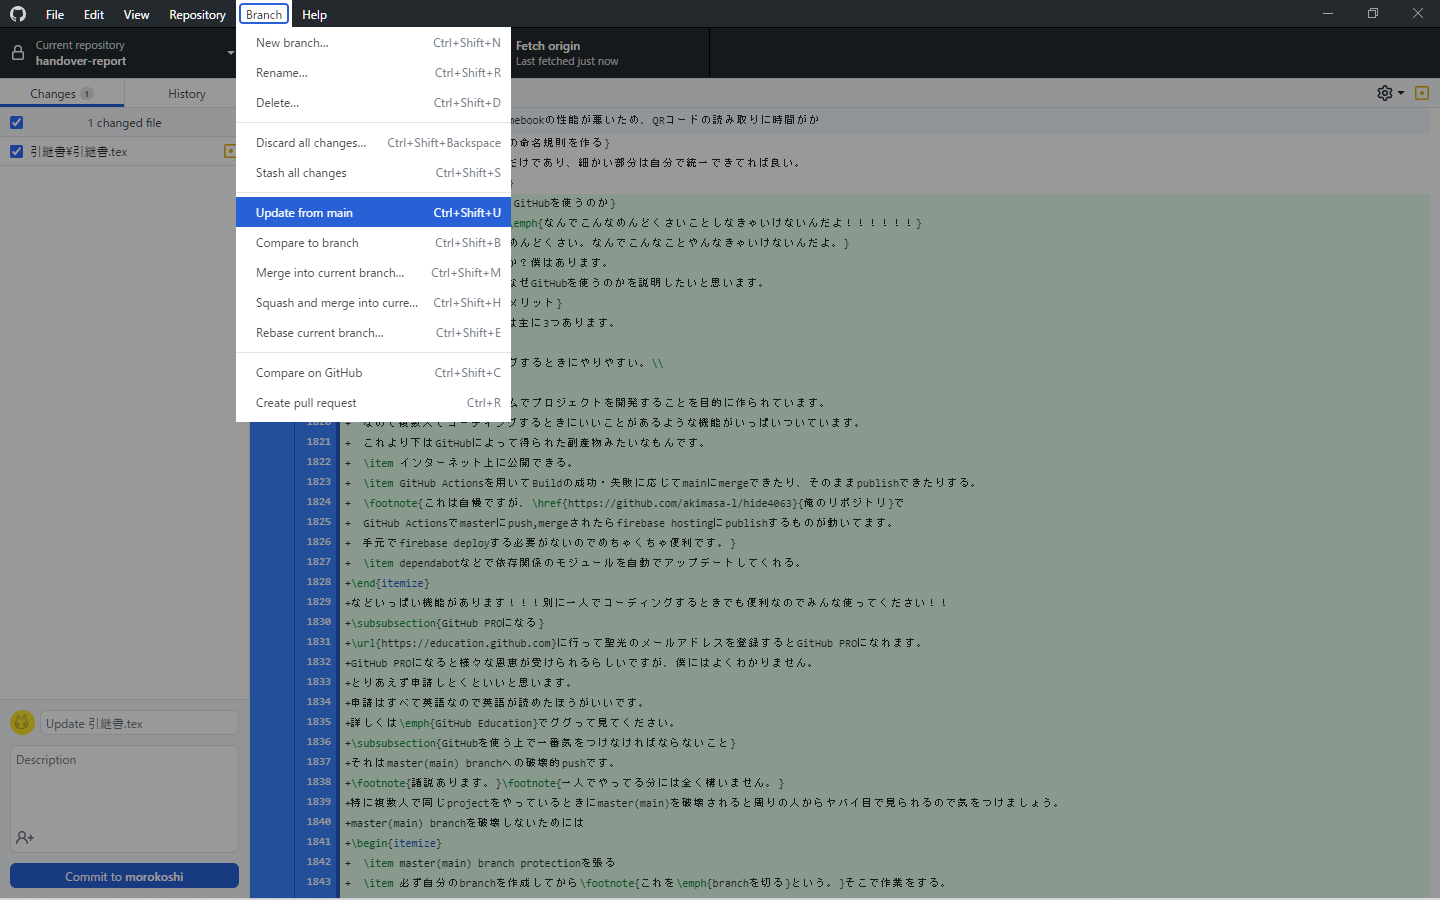
\includegraphics[width=15cm]{assets/update-branch.png}\\
GitHub Desktopでこんなかんじでmainと同じcommitまでできます!!
注意としては編集を始める前にこれをしないとconflictが生じちゃうので編集を始める前にこれをしましょう。
あとたまにテキストエディターで開いてるときだとできないこともあるのでテキストエディターを閉じているときにすると成功するかもしれません。
\subsubsection{GitHubに上げるべきもの・上げないべきもの}
GitHubにはコーディングの際に必要なものを上げるべきであるが、そのときに上げるべきもの、上げないべきものが存在する。
\subsubsubsection{GitHubに上げるべきもの}
GitHubに上げるべきものとして、
\begin{itemize}
  \item コード。\footnote{それはそう。}
  \item 各環境で共通しているもの(依存関係を記しているものなど)
  \item そのほかbuildに必要なもの
  \item .gitignore\footnote{ローカルの中だけでgitに上げたくないものがあれば
  .gitignoreの中に.gitignoreを入れることもありますが基本時にはcommitしたほうがいいでしょう。
  }
  \item LICENSE\footnote{基本的にはリポジトリを持っている人がイキって入れていることが多いです。特に意味はないと思います。}
\end{itemize}
があります。
\subsubsubsection{GitHubに上げないべきもの}
逆にGitHubに上げないべきものとして、
\begin{itemize}
  \item バイナリファイル(テキストエディタなどで読んでもぶわ\UTF{FF5E}\UTF{FF5E}\UTF{FF5E}って謎の文字列が並んでて読めないやつ)
  \footnote{画像ファイルなどのbuildに必要なやつは上げるべきです。
  しかしGitHubには一つのcommitにつき100MBまでの制限があるためクソ高画質な画像ファイルは上げられないので気をつけてください。
  できれば無限画質でかつファイルサイズが小さいsvgを使いましょう。
  }
  \item 依存環境などbuildによって生成される各環境によって生成されるものが異なると予想されるもの。
  \footnote{node.jsにおけるnode\_modulesなどがこれに当たります。}
  \item パスワードなどのプライベートなもの。
\end{itemize}
があります。
これらをGitHubに上げないためにはcommitする前に\emph{.gitignore}
にそれらのファイルを記入するとgitの管理下に置かれなくなります。
誤ってcommitしちゃったときは\emph{git commit 取り消し}でググってください。\subsubsection{Git周りのソフト}
\subsubsubsection{GitとGitHub}
そもそもGitとGitHubは違う。Gitはバージョン管理関係のコマンドソフトである。そしてそれをリモートで見れるようにしたのがGitHubである。私たちがGitHubを見るのに必要なものの一つがGitである。
\subsubsubsection{GitHub Desktop}
ローカルレポジトリでのコミット、プッシュ、プル、プルリク、ブランチ生成をUIで行えるソフト。純正。コマンドでやるのにこだわる場合、開発ソフトにGit連携機能がある場合を除いて入れとこう。
\subsubsection{Organization}
生徒会としてGitHubOrganizationを作った\footnote{https://github.com/SeikoStudentCouncil}。Organizationは複数のアカウントを所属させることができ、組織としてGitを使用できるというものである。管理者権限が欲しい場合は前年度局長または60227li@seiko.ac.jpに連絡すること。
\subsubsubsection{メンバー}
GitHubアカウント作った後に管理者はPeopleタブ>Memberからユーザーネームを検索し招待する。招待はメールでくるので受理して参加する。この時Roleを決めることができる。Roleは役職のことでありOwnerとMemberの2種類がある。
\subsubsubsection{チーム(Teams)}
チームは...そのままの機能。アプリ局とHP局というチームを作った。チームごとに見れるレポジトリを設定できたりする。
\subsubsection{レポジトリの作り方}
調べろ。空リモートレポジトリを作り、プリジェクトファイルをPushすれば完成。
\subsubsection{作業フローチャート}
 \begin{enumerate}
 \item 新機能や修正などのイシューを立てる(イシュータイトルは英語)
 \item イシュー番号がついたブランチを切る\\
 (ブランチ名:\verb|feature/#[イシュー番号]_[イシュータイトル(ケバブケース)]|)
 \item リモートレポジトリをPush/Fetchする
 \item 作業をする
 \item ひと段落したらCommitする
 \item 4, 5を繰り返す(数時間〜1日サイクル)
 \item ある程度できたらPushする
 \item 4〜7を繰り返す(1日〜3日サイクル)
 \item 機能が実装できたらブランチのプルリクをmainブランチに送る
 \item もし、訂正箇所や指摘があれば4まで戻る(コードレビューする)
 \item コードレビューが成功したらマージしてもらう
 \item イシューとブランチをClose(終了)する
 \item 最初に戻る
 \end{enumerate}
 もし、管理者が自分であってもなるべくこのフローチャートを崩さずにコーディングする。自分のコードをコードレビューしてもしょうがないのでここら辺は即マージで構わない。
 \subsubsection{コミットメッセージ(Commit Summery)}
 コミットのSummaryは以下の書式は\verb|[commitType] summary|とする。summary はコミットの内容を簡潔に英語でかく(ただし動詞で、パスカルケース、原形=命令形文法)。そして、commitTypeは以下から選ぶ。

\begin{itemize}
\item fix:バグ修正 
\item hotfix:致命的なバグの修正
\item add:新規(ファイル)機能追加
\item update:機能修正(バグではない)
\item change:仕様変更
\item clean:整理(リファクタリング等)
\item disable:無効化(コメントアウト等)
\item remove:削除(主にファイル)
\item upgrade:バージョンアップ
\item revert:変更取り消し
\end{itemize}
\subsubsection{.gitignoreについて}\label{sec:gitignore}
.gitignoreという名前のファイルを直下に置くとそこに記載されたファイルやフォルダーはgit更新の対象から外れる。つまりcommitやpushされなくなるということ。pushにはファイル容量制限があるので実行ファイルなどが存在する場合はこの点に注意すること。
\subsection{マークシート}
\subsubsection{使用するアプリケーション}
\begin{itemize}
 \item マークシートDIY {\color{red}(必須)}\\
 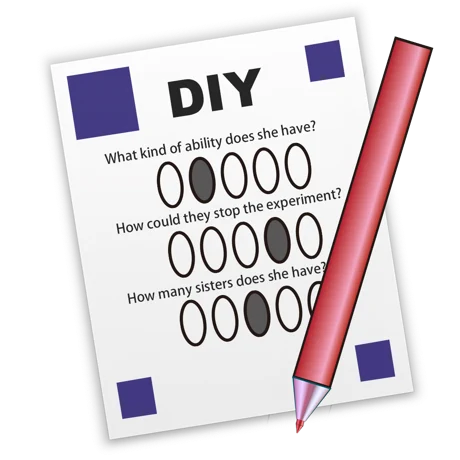
\includegraphics[width=5cm]{assets/answersheet-diy.png}\\
 \url{https://apple.co/3DgrhWp}\\
 マークシートを読み取るのに必要。
 \item \TeX Shop (任意)\\
 
\includegraphics[width=5cm]{assets/TeX.png}\\
 マークシート用紙を作るのに便利。\TeX が使えればなんでも良い。
\end{itemize}
 \subsubsection{マークシート用紙の作り方}
 \url{http://www7a.biglobe.ne.jp/~ogihara/ja/Manual_0.7.1ja.pdf}を見れば全てわかる。

 マークシートの四隅に位置決めマークが必要。そのうち左上のマークは他より大きい必要がある。

 以下は\TeX で用紙の作る方法を記す。\\
 \begin{enumerate}
  \item  マークする楕円と、用紙の四隅に位置決めマークを固定するためのパッケージをインポートする。\\
  \texttt{
  \textbackslash usepackage\{epic,eepic\}\\
  \textbackslash usepackage\{fancyhdr\}
  }
  \item 位置決めマークを挿入
  \begin{lstlisting}
   \pagestyle{fancy}
   \renewcommand{\headrulewidth}{1pt}
   \renewcommand{\footrulewidth}{0pt}
   \lhead{\rule{8mm}{8mm} {\huge アンケートタイトル}}
   \rhead{\rule{6mm}{6mm}}
   \lfoot{\rule{6mm}{6mm}}
   \rfoot{\rule{6mm}{6mm}}
   \chead{}
   \cfoot{}
   \end{lstlisting}
   任意のページのみに適用したい場合は1行目``pagestyle''を``thispagestyle''に変更する
  \item マーク欄を追加\\
  \begin{picture}(10,15) \put(3,3){\ellipse{10}{15}} \end{picture}と入力できる
  \begin{lstlisting}
  \begin{picture}(10,15)\\
  \put(3,3){\ellipse{10}{15}}\\
  \end{picture}\\
  \end{lstlisting}
  マーク欄の位置が合わない場合は、\texttt{put($n$,$n$)}の値を微調整すること。
  \item 3を繰り返して完成!
 \end{enumerate}
 \subsubsection{読み取り方}
 \url{http://www7a.biglobe.ne.jp/~ogihara/ja/Manual_0.7.1ja.pdf}を参照。\\
 \newpage
 \subsection{\TeX}
  \subsubsection{\TeX とは}
  PDFを作るためのプログラミング言語みたいなもの。\\
  \TeX を使うには専用のアプリケーションが必要だが、代表的なものとしてTeXShop\footnote{三枝と李が使用}やAtom\footnote{飼沼が使用}がある。
  \subsubsection{ダウンロード}
  ここではTeXShopのMacOSでのインストールについて述べる。\\
  以下からpkgファイルがダウンロードできる。\\
  \url{https://tug.org/mactex/mactex-download.html}
  \subsubsection{Mac\TeX の日本語設定}
  \TeX は導入が一番大変。ここさえ乗り越えれば大丈夫。\\
  Mac\TeX をインストールしただけでは、うまく日本語を扱うことができない。和文文書を作成するための準備が必要。\\
  設定にはターミナル\footnote{\texttt{/Applications/Utilities/Terminal.app}にある。Finderで\texttt{Command + Shift + U}を押して「ユーティリティ」フォルダを開き、「ターミナル」アプリをダブルクリックするのが簡単だろう}でコマンドを打ち込む必要がある。
  \subsubsubsection{tlmgr を用いたアップデート}
  \TeX Liveレポジトリの内容を最新版に更新するため、次のコマンドを打ち込む。\footnote{管理者ユーザでの実行が前提}
  \begin{lstlisting}
   sudo tlmgr update --self --all
  \end{lstlisting}
  パスワードが必要。\footnote{このとき、セキュリティ上の理由により、打ち込んだパスワードは画面に一切表示されない。パスワード文字数が見えてしまうのを防ぐため、****のようなマスク文字も表示されない。まるでキーボードが効いていないかのように見えるが、入力はされているので、そのままパスワードを最後まで打ち込んで、returnキーを押す。なお、sudoは管理者権限を用いて実行するためのコマンドです。一度実行すると、それからしばらくの間はパスワードなしでsudoを連続実行できます。}
  \subsubsubsection{ヒラギノフォントの準備}
  続いて、MacOSに標準で用意されているヒラギノフォントを\TeX で使用するため、次ページのコマンドを実行する。一行ずつ順番に実行すること。
  \newpage
  \begin{lstlisting}
sudo mkdir -p /usr/local/texlive/texmf-local/fonts/opentype/screen/hiragino
cd /usr/local/texlive/texmf-local/fonts/opentype/screen/hiragino
sudo ln -s "/Library/Fonts/ヒラギノ明朝 Pro W3.otf" HiraMinPro-W3.otf
sudo ln -s "/Library/Fonts/ヒラギノ明朝 Pro W6.otf" HiraMinPro-W6.otf
sudo ln -s "/Library/Fonts/ヒラギノ丸ゴ Pro W4.otf" HiraMaruPro-W4.otf
sudo ln -s "/Library/Fonts/ヒラギノ角ゴ Pro W3.otf" HiraKakuPro-W3.otf
sudo ln -s "/Library/Fonts/ヒラギノ角ゴ Pro W6.otf" HiraKakuPro-W6.otf
sudo ln -s "/Library/Fonts/ヒラギノ角ゴ Std W8.otf" HiraKakuStd-W8.otf
sudo ln -s "/System/Library/Fonts/ヒラギノ明朝 ProN W3.otf" HiraMinProN-W3.otf
sudo ln -s "/System/Library/Fonts/ヒラギノ明朝 ProN W6.otf" HiraMinProN-W6.otf
sudo ln -s "/Library/Fonts/ヒラギノ丸ゴ ProN W4.otf" HiraMaruProN-W4.otf
sudo ln -s "/System/Library/Fonts/ヒラギノ角ゴ ProN W3.otf" HiraKakuProN-W3.otf
sudo ln -s "/System/Library/Fonts/ヒラギノ角ゴ ProN W6.otf" HiraKakuProN-W6.otf
sudo ln -s "/Library/Fonts/ヒラギノ角ゴ StdN W8.otf" HiraKakuStdN-W8.otf
\end{lstlisting}
  \subsubsubsection{游フォントの準備}
  OSX 10.9 Mavericks以降では,字游工房の高品質な游フォント(游明朝体・游ゴシック体)も用意されている。これも\TeX から使えるようにしておく。次の一連のコマンドを実行する。
  \begin{lstlisting}
sudo mkdir -p /usr/local/texlive/texmf-local/fonts/opentype/jiyukobo/yu
cd /usr/local/texlive/texmf-local/fonts/opentype/jiyukobo/yu
sudo ln -s "/Library/Fonts/Yu Mincho Medium.otf" YuMin-Medium.otf
sudo ln -s "/Library/Fonts/Yu Mincho Demibold.otf" YuMin-Demibold.otf
sudo ln -s "/Library/Fonts/Yu Gothic Medium.otf" YuGo-Medium.otf
sudo ln -s "/Library/Fonts/Yu Gothic Bold.otf" YuGo-Bold.otf
  \end{lstlisting}
  \subsubsubsection{仕上げ}
  仕上げに、次のコマンドを実行する。デフォルトでヒラギノフォントが埋め込まれた PDFが作成されるようになる。
  \begin{lstlisting}
sudo mktexlsr
sudo kanji-config-updmap-sys hiragino-pron
  \end{lstlisting}
  また、
  \begin{lstlisting}
  kanji-config-updmap-sys status
  \end{lstlisting}
  を実行して、現在使用可能なフォント設定を確認できる。
  \subsubsubsection{TeXShopの日本語設定}
  TeXShopを開いて、メニューから「環境設定」を開く。\\
  設定画面が現れるので左下の「設定プロファイル」をクリックする。\\
  Unicode を活用できるup\LaTeX を使用する場合は\texttt{upTeX(ptex2pdf)}を,従来の p\LaTeX を使用する場合は\texttt{pTeX(ptex2pdf)}というプロファイルを選択する。\footnote{この引き継ぎ書は後者を使っている。基本的には後者での設定を推奨する}\\
  プロファイル変更を終えたら、OKボタンを押して環境設定を確定させ、TeXShop を終了する。
  その後,ターミナルで次のコマンドを実行しておきましょう。\footnote{1行目は、古いOS X において,行番号がスクロールしないOS側のバグに対処するための対症療法を停止させる措置。最近のMac OSではこのバグが修正されていますので,この対症療法は不要。対症療法が残っていると,スクロール速度が遅くなる原因となる。\\2行目は、スクロール時に上下端で大きく跳ね返るバウンスエフェクトを停止させる措置。3行目は、プレビューウィンドウのPDFが一部の環境でぼやけて見えてしまうのを防止する措置。}
  \begin{lstlisting}
defaults write TeXShop FixLineNumberScroll NO
defaults write TeXShop SourceScrollElasticity NO
defaults write TeXShop FixPreviewBlur YES
  \end{lstlisting}
  あとはTeXShopを再起動すれば準備完了。
  \subsubsection{推奨設定}
  以下は全てTeXShopの環境設定のウィンドウからできる。
  \subsubsubsection{エディターのフォント}
  上部の「書類」タブの「フォント」からエディターのフォントをヒラギノ角ゴシックなどの日本語に最適なゴシックフォントを設定する。
  \subsubsubsection{新しいファイルの自動作成}
  上部の「書類」タブの「起動時に」の「新しいファイルを作成する」のチェックボックスをはずす。
  \subsubsubsection{ソースコードとプレビューの統合}
  上部の「プレビュー」タブの「ソースとプレビューの開き方」で設定できる。
  \subsubsubsection{キーバインド}
  \TeX で文章を書くときに必須の設定。\\
  これを設定するだけで作業効率が格段に上がる。\\
  上部の「エディタ」タブの「エディタ」の「キーバインド」にチェックをつける。\\
  「キーバインド」はショートカットのようなもので、自分の好みの設定できる。カスタマイズはTeXShopのメニューバーの「ソース」>「キーバインドファイルの編集」を押すとキーバインド一覧が表示されるので、好きなように追加したり削除したりしてカスタマイズできる。
  \subsubsubsection{スペルチェック}
  上部の「書類」タブの「スペルチェック」の「\TeX コマンドを対象外にする」と「特定のコマンド引数を対象外にする」のチェックボックスをつけてオンにする。
  \subsubsection{書き方}
  この引き継ぎ書自体もそうだが、技術局ドライブに\TeX ファイルがいっぱいあるのでそれを参考にしてほしい。あとは大概Google検索で出てくる。
  \subsection{SpreadSheet$\sqrt{大全}$}
  ここはSpreadSheetの使い方を大全とはいかなくとも、全ての機能のうちその平方根\footnote{``知識は足し算ではなく掛け算だ''と誰かが言っていたため、もう半分学べば全てのことはできるだろうと言うこと。ちなみにスプレッドシートを完全に使いこなせる人はいないし、その必要はない。}ぐらいは解説しようというコーナーである。なるべく日本語を消して書くことにする。また、初心者用ではないのでわからない場合は$n$回読むこと。以下、スプレッドシートファイルをgsh、スプレッドシート内のシートのことをgssと書くことにする。
  \subsubsection{基本操作}
  
  {\small
\begin{center}
\begin{tabular}{|
>{\columncolor[HTML]{CCCCCC}}l |
>{\columncolor[HTML]{FFF2CC}}l |
>{\columncolor[HTML]{F3F3F3}}p{10cm} |}
\hline
\multicolumn{1}{|c|}{\cellcolor[HTML]{CCCCCC}\textbf{命令}} &
  \multicolumn{1}{c|}{\cellcolor[HTML]{CCCCCC}\textbf{キー}} &
  \multicolumn{1}{c|}{\cellcolor[HTML]{CCCCCC}\textbf{説明}} \\ \hline
\textbf{保存} &
  Ctrl + S &保存をしないと変更した内容が記録されず消えてしまいます。スプレッドシートでは自動保存機能がありますが、他のソフト等では十分気を付けて下さい。合言葉は「5秒に1回Ctrl+S」です。 \\ \hline
\textbf{コピー}             & Ctrl + C    & 選択したセル、文字をクリップボードにコピーします。クリップボードとはパソコンの中にある見えない領域です。そこに値を一時的に保存しています。 \\ \hline
\textbf{切り取り} &
  Ctrl + X &
  選択したセル、文字をクリップボードに移動させます。コピーとは違ってもともとあった値は削除されます。ですが、スプレッドシートでは挙動が難しいので基本的にコピーして貼り付けてから削除をすることをお勧めします。 \\ \hline
\textbf{貼り付け}            & Ctrl + V    & クリップボードから値を貼り付けます。クリップボードの中の値は保持されたままなのでクリップボードが上書きされるまで何回でも貼り付けできます。 \\ \hline
\textbf{保持値のみ貼り付け} &
  Ctrl + Shift + V &
  コピーしたセルの保持値のみを貼り付けます。書式と数式は無視されます。書式が固められてるスプレッドシートではこれを使うようにしてください。 \\ \hline
\textbf{検索}              & Ctrl + F    & キーワードで検索ができます。                                                        \\ \hline
\textbf{検索と置換}           & Ctrl + H    & 検索のオプションを追加できたり、ヒットした部分を別の文字に置き換えることもできます。                            \\ \hline
\textbf{すべて選択}           & Ctrl + A    & すべてを選択します。                                                            \\ \hline
\textbf{元に戻す}            & Ctrl + Z    & 1つ前の状態に戻します。複数回使用することで何回でも前に戻せますが、限界はあります。                            \\ \hline
\textbf{やり直し}            & Ctrl + Y    & 1つ後の状態にします。元に戻しすぎたときに元に戻すのを戻せます。                                      \\ \hline
\textbf{編集}              & Enter       & セル選択状態でEnterを押すと                                                      \\ \hline
\textbf{選択}              & Ctrl + 左    & Ctrlを押しながらセルをクリックするともともと選択されたセルや範囲に加えて選択されます。                         \\ \hline
\textbf{範囲選択}            & Shift + 左   & Shiftを押しながらセルをクリックするともともと選択されたセルを始点、クリックされたセルを終点とした範囲が選択されます。         \\ \hline
\textbf{\begin{tabular}[c]{@{}l@{}}セルを移動\\ (選択状態)\end{tabular}} &
  ←↑→↓ &
  矢印キーの方向に移動できます。Shiftを押しながら移動することで範囲選択をすることもできます。 \\ \hline
\cellcolor[HTML]{CCCCCC} & Tab         & 右                                                                     \\ \cline{2-3} 
\cellcolor[HTML]{CCCCCC} & Shift + Tab & 左                                                                     \\ \cline{2-3} 
\cellcolor[HTML]{CCCCCC} & Enter       & 下                                                                     \\ \cline{2-3} 
\multirow{-4}{*}{\cellcolor[HTML]{CCCCCC}\textbf{\begin{tabular}[c]{@{}l@{}}セルを移動 \\(入力状態)\end{tabular}}} &
  Shift + Enter &
  上 \\ \hline
\end{tabular}
\end{center}
}
  \subsubsection{セル}
  \subsubsubsection{セル座標}
  横軸を列、縦軸を行と呼び、表記は$列:行$。左から3列目、上から4行目は$C:4$である。このような表記のことをセル座標ということにする。セル座標はセルの値を指すこともあるが、あくまでセルを表す。
\\
  また、あるセルAでそれと異なるセルBのセル座標を数式で指定した場合、AからBの相対位置が保存されるため、AFやコピーによってAのセルを変更すると以前の相対位置を保つようにBも変更される。
  \subsubsubsection{セルの理解}
  セルは三つに分けて考えると簡単。ちなみに専門用語ではないし、李の勝手な解釈。
  \begin{itemize}
  \item 入力値\\
  ユーザが入力した純粋な文字列
  \item 内部値(保持値)\\
  入力値を演算した結果の値
  \item 書式\\
  セル及び内部値の表示を装飾する機能全般
  \end{itemize}
  ちなみに、スプレッドシート講座テキストというgshに書いてあることから少し変更した。
  \subsubsubsection{セルのコピペ}
  セルを選択した状態でコピー(Ctrl[Command] + C)または切り取り(Ctrl[Command] + X)すると入力値及び書式がコピーされる。そのままペースト(Ctrl[Command] + V)すると、入力値及び書式がペーストされる。値のみペースト(Ctrl[Command] + Shift + V)すると内部値のみペーストされる。
  \\
  なお、入力値がペーストされその中に相対セル指定があった場合、以前の相対位置を保つように相対セル指定が変わる。
  \subsubsection{権限}
  \subsubsubsection{野良スプレッドシートの場合}
  どこの共有ドライブにも所属していない(つまりマイドライブにある)gshを野良gshと呼ぶことにする。
 共有設定には大きく分けて二種類あり、リンク共有と招待共有である。リンク共有はリンクを用いた共有方法で、URLを別の手段で送信したり掲示したりするときに使用する。リンク共有の場合は不特定多数の人がアクセスできる可能性があるので条件で権限を付与できる。「誰」がgshで「何を」できるかを設定することができる。
 \begin{itemize}
 \item 誰が
 \begin{itemize}
 \item 制限付き\\
 招待共有のみにする
 \item 聖光学院中学校高等学校\\
 我が校は独自ドメインを作っているのでドメイン内のすべてのGoogleアカウントが対象となる
 \item リンクを知ってる全員\\
 誰でもアクセス可能
 \end{itemize}
 \item 何を
 \begin{itemize}
 \item 閲覧者\\
 閲覧できる
 \item 閲覧者(コメント可)\\
 コメントできる
 \item 編集者\\
 編集できる
 \end{itemize}
 \end{itemize}
 招待共有ではGmailアカウント一個ごとに招待や権限設定を行える。権限設定は上記の「何を」の部分と完全に一致するが、あなたがオーナー権限の場合はオーナーを移譲できる。(後述)なお、招待共有とリンク共有がある個人について同時に設定されていた場合、場合、閲覧者\verb|<| 閲覧者(コメント可)\verb|<| 編集者\verb|<| オーナーの順で優先されるので"みんな編集OKだけどいつは閲覧だけ"という設定はできない。
 \\
 
 また招待共有をする際、相手側にメールを送るかどうかを設定できる。送る場合は文章も送ることができる。相手側に知らせるために送る方がいいだろう。リンク共有はあたりまえだが、メールを送ることはできない。
 \\
 
 そして、これは一度も使ったことないどころかこのコーナーを書くためにgshの機能をぽちぽちしてたときに見つけたのだが、共有設定の右上の歯車で、閲覧者によるgshのダウンロードやコピー、印刷を防ぐ設定をすることができるらしい。
 \subsubsubsection{共有ドライブに入っている場合}
 共有ドライブに所属している場合、基本的に野良と変わりはないが、「招待共有に所属フォルダーの権限が引き継がれる」という違いがある。このgshが所属しているフォルダーに設定された権限はデフォルトとして、最初から招待共有されている。これによってデフォルトで権限を持っているユーザはメンバー、新しく追加した人はゲストと呼称される。メンバーを削除することや編集することはできない。ゲストとして新しく招待した人は編集もできる。正直このくそ仕様を早く変えてもらいたいが、だったらショートカット使えと言われそう。\footnote{ショートカットも結構クソなのでできるだけ使いたくない。}
 
 \subsubsection{書式}
 \subsubsubsection{文字に関する書式}
 \begin{itemize}
 \item テキストの色\\
 文字の色を変える。一部だけ変えることもできる。
 \item 太字\\
 Ctrl[Command] + B。太文字にすることができる。一部だけ変えることもできる。
 \item 斜体\\
 Ctrl[Command] + I。イタリック体にすることができる。一部だけ変えることもできる。
 \item 下線\\
 Ctrl[Command] + U。下線をつけることができる。一部だけ変えることもできる。メニューにないので表示形式タブから設定すること。
 \item 取り消し線\\
 Ctrl[Command] + Shift + X。取り消し線をつけることができる。一部だけ変えることもできる。
 \item フォントサイズ\\
 文字の大きさを変えることができる。単位はpt。
  \item 水平方向の配置\\
 左、中央、右寄せができる。
 \item 垂直方向の配置\\
 上、中央、下寄せができる。
 \item テキストを折り返す\\
 テキストがセルを越したときにどう表示するかを選べる。
 \begin{itemize}
 \item はみ出す\\
 セルを超えて表示する。
 \item 折り返す\\
 セル内で折り返す。
 \item 切り詰める\\
 セルを超えた文字は表示しない。
 \end{itemize}
 \item テキストの回転\\
 いろんな角度に設定することができる。数字で回転度数も設定できる。
 \item リンクを挿入\\
 Ctrl[Command] + K。セル内の文字にリンクを挿入できる。
  \item フォント\\
  フォントを変えることができる。とりあえずNoto Sans使っとけ。
  \item 表示書式\\
  書式の中でもっとも大切な要素。あとで別途取り上げる。
 \end{itemize}
 
 \subsubsubsection{セルに関する書式}
 \begin{itemize}
 \item セルを結合\\
 セルを結合できる。その際、結合方式を選ぶことができる。
 \begin{itemize}
 \item すべて結合\\
 選択した範囲をすべて結合
 \item 縦方向に結合\\
 選択した範囲のうち、縦方向にだけ結合する。
  \item 横方向に結合\\
 選択した範囲のうち、横方向にだけ結合する。
  \item 結合を解除\\
 すべての結合を解除。
 \end{itemize}
 \item コメントを挿入\\
  Ctrl[Command] + Alt[Option] + M。セルにコメントを付けられる。後述。
   \item 塗りつぶしの色\\
 背景色を変えることができる。
  \end{itemize}
  \subsubsubsection{その他の書式}
  \begin{itemize}
  \item 条件つき書式\\
  条件をもとに書式を変えることができる。例えば、「空白のセルの背景を変える」ことができる。ここで長々と説明するより、体験した方が早い。
  \end{itemize}
\subsection{Brother Print SDK}\label{sec:Brother Print SDK}
第62回聖光祭で購入したBrotherのラベルプリンタQL-810WにiPadで接続する方法と、SDKを使ってオリジナルのiPad Appから印刷できるようにする。\\
公式ドキュメントが分かりづらい\& 日本企業のくせにほとんど翻訳されていないので、以下に記す。
 \subsubsection{導入}
  \subsubsubsection{ダウンロード}
  まずはSDKのダウンロードといきたいところだが、Brother Japanの開発者向けホームページの\link{``モバイルSDKとは?''}{https://support.brother.co.jp/j/s/es/dev/ja/mobilesdk/index.html?c=jp&lang=ja&navi=offall&comple=on&redirect=on}にあるダウンロードをクリックすると謎のサインインを要求される。 \\
  一方、なぜだかわからないが、Brother(US)の同じホームページ\link{``What is a Mobile SDK?''}{https://support.brother.com/g/s/es/dev/en/mobilesdk/index.html?c=eu_ot&lang=en&navi=offall&comple=on&redirect=on}で\link{``Mobile SDK Download''}{https://support.brother.com/g/s/es/dev/en/mobilesdk/download/index.html?c=eu_ot&lang=en&navi=offall&comple=on&redirect=on}をクリックすると普通にダウンロードページが表示されるので、``Brother Print SDK for iPhone/iPad''をダウンロードする。\\
  生徒会が所有しているQL-810Wは海外向けモデルなので海外版を使っても問題ない。
 \subsubsubsection{プロジェクトにSDKを追加する}
  ダウンロードした``bpsdkiall(バージョン番号)''のフォルダ\footnote{zipでダウンロードされるがMacOSなので自動解凍されるはず}下の同じ名前のzipファイルを展開し、作成されたフォルダ内を開く。``libs''>``Net''内の``BRLMPrinterKit.framework''フォルダをコピーして、導入先のプロジェクトのフォルダの``.xcodeproj''ファイルと同じ階層にペーストする。\\
  Xcode Projectを開いて、プロジェクトのトップの``General''の``Frameworks, Libraries, and Embedded Content''にある+ボタンを押して、``Add Other...''>``Add Files...''を選択して先ほどペーストした``BRLMPrinterKit.framework''のフォルダを選択する。\\
  次に、\texttt{Info.plist}のリストの外の任意のところを右クリックして``Add Row''をクリックし、\texttt{Supported External Accessory Protocols}と入力する。追加した\texttt{Supported External Accessory Protocols}を展開し、\\値に\texttt{com.brother.ptcbp}を設定する。\\
  同様にして、\texttt{Info.plist}に\texttt{Privacy - Local Network Usage Description}と\texttt{Bonjour services}を追加する。追加した\texttt{Privacy - Local Network Usage Description}の値にアプリで必要な理由を設定し、\texttt{Bonjour services}には
  \begin{itemize}
  \item \EscVerb{_pdl-datastream._tcp}
  \item \EscVerb{_printer._tcp}
  \item \EscVerb{_ipp._tcp}
  \end{itemize}
  の3つを設定する。
  \subsubsubsection{Product Plan IDの取得}
  MFi 対応プリンター向けアプリケーションをApp Storeで公開する場合、Product Plan ID (PPID) を取得する必要があります。 PPID を取得するためには\link{MFi対応プリンター向けアプリケーション認証プロセス}{https://online.brother.co.jp/dev/MFiTop.aspx}を参照。
  \subsubsubsection{App Storeへリリースする際の注意点}
  \texttt{BRLMPrinterKit.framework}を含んだアプリケーションをApp Store (TestFlight)へ公開する場合には、 下記コマンドを実行してシミュレータ用のアーキテクチャ(\verb|i386|,\verb|x86_64|)をFrameworkから除外する必要がある。\\
  下記コマンド(ディレクトリ)とは``BRLMPrinterKit.framework''を内包しているフォルダのパスを意味する。
  \begin{lstlisting}
$ lipo -remove i386 (ディレクトリ)/BRLMPrinterKit.framework/BRLMPrinterKit -o (ディレクトリ)/BRLMPrinterKit.framework/BRLMPrinterKit
$ lipo -remove x86_64 (ディレクトリ)/BRLMPrinterKit.framework/BRLMPrinterKit -o (ディレクトリ)]/BRLMPrinterKit.framework/BRLMPrinterKit
  \end{lstlisting}
  また、下記コマンドを実行することで、シミュレータ用のアーキテクチャ(\verb|i386|,\verb|x86_64|)が除外されていることを確認できる。
  \begin{lstlisting}
$ lipo -info [your current directory]/BRLMPrinterKit.framework/BRLMPrinterKit
  \end{lstlisting}
  \subsubsubsection{Xcode 12で発生するビルドエラー解消}
  ``BRLMPrinterKit.framework''を含んだアプリケーションをXcode 12以上を使ってビルドするとき、下記のようなエラーメッセージが表示されてビルドに失敗する場合、エラーを解消できる方法を記す。
  \begin{enumerate}[ケース1]
   \item ``Building for iOS, but the linked and embedded framework `BRLMPrinterKit.framework' was built for iOS + iOS Simulator''\\
   ``Build Settings''内の``Validate Workspace''の設定を\texttt{Yes}にしてビルドする。 \\
   その後、``Validate Workspace''は\texttt{Yes},\texttt{No}のいずれでもよいが、ビルド結果が異なる。
   \begin{itemize}
    \item \texttt{Yes}のまま\\
    ワーニングが発生しますが、アプリケーションのビルドは成功する。
    \item \texttt{No}を選択\\
    エラーもワーニングも発生することなくアプリケーションのビルドに成功する。
   \end{itemize}
   \item ``Building for iOS Simulator, but linking in dylib built for iOS''\\
   \texttt{arm64}をプロジェクトのシミュレータアーキテクチャから除外する。\\
    ``Build Settings''内の``Excluded Architecture""を\texttt{arm64}で指定し、 \texttt{Any iOS Simulator SDK}を追加する。
   \item Apple Siliconを搭載したMacでエラーが出る\\
   Xcodeを終了し、Finderから``アプリケーション''フォルダを開いて、``Xcode.app''を右クリックして、``情報をみる''をクリックする。ウィンドウが表示されるので``Rosettaを使用して開く''のチェックボックスをオンにして、Xcodeを再起動する。
  \end{enumerate}
  \subsubsection{サンプルコード}
   \subsubsubsection{画像やPDFを印刷する}
   \lstset{language=swift}
   \begin{lstlisting}
func printPDF(path: URL) {
    let channel = BRLMChannel(wifiIPAddress: "/* プリンターのIPアドレス */")

    let generateResult = BRLMPrinterDriverGenerator.open(channel)
    guard generateResult.error.code == .noError,let printerDriver = generateResult.driver else {
            print("Error - Open Channel: \(generateResult.error.code)")
            return
    }
    defer {
        printerDriver.closeChannel()
        print("channel closed")
    }
    guard let url = Bundle.main.url(forResource: "YourImageFilename", withExtension: "Extension"),
        let printSettings = BRLMQLPrintSettings(defaultPrintSettingsWith: .QL_810W)
        else {
            print("エError - Image file is not found.")
            return
    }

    printSettings.labelSize = .dieCutW23H23 /* ラベルサイズ */
    printSettings.autoCut = false  /* 1ページずつカットをオフ */
    printSettings.cutAtEnd = true  /* PDFの全ページを印刷してまとめてカット */
    printSettings.hAlignment = .center /* 縦方向の揃え方 */
    printSettings.vAlignment = .center /* 横方向の揃え方 */
    printSettings.scaleMode = .fitPageAspect  /* ページギリギリまでコンテンツを拡大する */

    let printError = printerDriver.printImage(with: path, settings: printSettings)

    if printError.code != .noError {
        print("Error - Print Image: \(printError.code)")
    }
    else {
        print("Success - Print Image")
    }
}
   \end{lstlisting}
   \subsubsubsection{プリンターを検索する}
   このAPIは第62回聖光祭では使用していないが、使用を推奨する。
   \begin{lstlisting}
class YourClass/* クラス名 */: NSObject, BRPtouchNetworkDelegate {
    private var networkManager: BRPtouchNetworkManager?

    func startSearchWiFiPrinter() {
        let manager = BRPtouchNetworkManager()
        manager.delegate = self
        manager.startSearch(5)
        self.networkManager = manager
    }

    // BRPtouchNetworkDelegate
    func didFinishSearch(_ sender: Any!) {
        guard let manager = sender as? BRPtouchNetworkManager else {
            return
        }
        guard let devices = manager.getPrinterNetInfo() else {
            return
        }
        for deviceInfo in devices {
            if let deviceInfo = deviceInfo as? BRPtouchDeviceInfo {
                print("Model: \(deviceInfo.strModelName), IP Address: \(deviceInfo.strIPAddress)")
            }
        }
    }
}
   \end{lstlisting}
  \subsubsection{API}
   \subsubsubsection{BRLMQLPrintSettingsLabelSize}
   印刷するラベルサイズを指定するオプション
   \begin{itemize}   
     \item DieCutW17H54
     \item DieCutW17H87
     \item DieCutW23H23
     \item DieCutW29H42
     \item DieCutW29H90
     \item DieCutW38H90
     \item DieCutW39H48
     \item DieCutW52H29
     \item DieCutW62H29
     \item DieCutW62H100
     \item DieCutW60H86
     \item DieCutW54H29
     \item DieCutW102H51
     \item DieCutW102H152
     \item DieCutW103H164
     \item RollW12
     \item RollW29
     \item RollW38
     \item RollW50
     \item RollW54
     \item RollW62
     \item RollW62RB
     \item RollW102
     \item RollW103
     \item DTRollW90
     \item DTRollW102
     \item DTRollW102H51
     \item DTRollW102H152
    \end{itemize}
\newpage  
\subsection{GoogleAppsScript$\sqrt{大全}$}
ここはGoogleAppsScript(以下、GASとする)の使い方を大全とはいかなくとも、全ての機能のうちその平方根ぐらいは解説しようというコーナーである。初心者用ではないのでわからない場合は$n$回読むこと。
\subsubsection{概要}
GASはGoogleWorkspaceをはじめとしたGoogleサービス、そしてHTMLやデータの基本処理を行うことを目的としたアプリケーション開発プラットフォームである。開発は全てブラウザで完結しており、Googleアカウントと結び付けられたProjectファイルにクライアント環境を選ばずアクセスができる。
\subsubsection{できること}
以下はGAS公式リファレンスに載っている、GASができることのリストを意訳したものである。
\begin{itemize}
\item Googleドキュメント、スプレッドシート、フォームにカスタムメニューやダイアログ、サイドバーなどの新機能を追加する。
\item Googleスプレッドシートにカスタム関数とマクロを追加する。
\item Googleサイトに埋め込まれたウェブアプリを公開する
\item AdSense、アナリティクス、カレンダー、ドライブ、Gmail、マップなどの他のGoogleサービスと連携する
\item Googleドキュメント、スプレッドシート、スライド、フォームのアドオンを開発及び公開する
\item AndroidアプリをAndroidアドオンとしてビルドし、クライアントでのGoogleドキュメント、スプレッドシートの情報を扱う
\item チャットbotを制作し、Googleチャットのワークフローを合理化する
\end{itemize}
\subsubsection{エディタ}
GASは2020年ぐらい\footnote{覚えてない。}にブラウザエディタを刷新しており、旧エディタでしか使えない機能などがあるかわり、新機能が追加されたりなど、かなり互換性が悪い。少し古い記事では旧エディタで作業をおこなっていたりするのでこの点に留意すること。なお、旧エディタと新エディタは切り替えが可能。
\subsubsection{開発言語}
GASはJavascriptを用いた開発が主流である。しかし、htmlファイルをサポートしており、GASでWebサイトを作る際はこれを使用する。
\subsubsection{GASの基本事項}
\subsubsubsection{GASの開き方}
GoogleAppsScriptと調べてもすぐにはエディタにたどり着けない。スプレッドシートから飛ぶやりかたを紹介されがちだが、面倒なので\url{https://script.google.com/u/0/home}からアクセスし、ブックマークに登録しとく方がいいだろう。
\subsubsubsection{GCPとの連携}
GoogleCloudPlatformというサービスがGoogleにはあり、GoogleにおいてのすべてのCloudサービスと連携が取れる。私も詳しくは理解していないが、Googleが提供しているクラウドコンピューティングサービスの総称ということらしい。開発中、ログを出したりそれを検証したりすると思うが、通常ではそれはできない。\footnote{前までは見ることができた。}GASプロジェクトとGCPを紐付けし、GCP内のログエクスプローラーを利用しなければならない。GCPとの連携方法は以下を参照。
 \begin{enumerate}
 \item GCPを開く
 \item 左上のプロジェクト名から新しいプロジェクトを押下
 \item プロジェクト名、組織(seiko.ac.jpでOK)、場所を設定して作成
 \item しばらくするとプロジェクトの作成が完了するので左上のハンバーガーメニューを選択
 \item APIとサービス \verb|>| OAuth同意画面へ
 \item UserTypeを内部(もし外部向けだった場合は外部)に設定し作成
 \item 必要な情報を入力。なお、必須項目だけでよい
 \item スコープは必要ない
 \item ダッシュボードにもどり、ハンバーガーメニューからホームへ
 \item プロジェクト番号をGASの設定のGCPの項目に入力
 \item 紐付け完了の通知が来たら終わり
 \end{enumerate}
 これはログエクスプローラーを使用するのに必要最低限の設定であり、GCPの別のサービスを利用する際はスコープなどを設定する必要が出てくることに注意。
 \\
 
ログエクスプローラーではクエリ言語を用いて、流れてくるすべてのログから必要なログを絞り込む必要がある。UIでサポートしてくれるのでクエリをクリアして必要な条件を選ぶだけで大丈夫。
\subsubsubsection{マクロ}
スプレッドシートのマクロを利用するとGASが自動生成される。このようなGASプロジェクトはスプレッドシートと紐付けされているという点で普通のスプレッドシートとは違う。紐付けされたプロジェクトは\verb|.getActive()|関数で編集中のスプレッドシートを指定できたり、紐付けされたスプレッドシートに限定された機能を実装できる。
\\

同様に、フォームやドキュメントなどと紐付けされたプロジェクトを作成することができる。とくにフォームと紐付けされたプロジェクトではフォームの回答を関数発火のトリガーとすることができる。

\subsubsubsection{実行方法そしてデプロイ}
出来上がったスクリプトはいろんな方法で実行することができる。
\subparagraph{実行}
関数の実行はすぐにできる。タブバーから実行したい関数名を指定して実行ボタンorデバッグボタンを押すだけで実行できる。スプレッドシートと紐付けされるとマクロの実行をすると関数が実行されたりする。

\subparagraph{トリガー}
トリガータブから設定できるトリガー。任意のバージョンの関数を時間を指定して実行できる。特定の日時を指定できたり、分単位から月単位で繰り返すこともできる。唯一注意すべきなのは日付ベースに設定した場合、指定できるのは1日の1時間の間だけであるということだ。つまり、1時にしていすることはできず、1時から2時までという感じでしか指定できない。
\\

もし毎日1時10分という感じで指定したいのであれば関数で次の日の現在時刻にトリガーを設定しその関数を次の実行で呼ぶという形で半永久的にトリガーを設定し続けることで実現できる。調べれば出てくるとは思うのでコードは省略する。

\subparagraph{デプロイ}
デプロイとはトリガーを外面的にし、いわばプログラムを``リリース''することである。GASには以下の4つのデプロイ方法をとることができる。
\begin{itemize}
\item ウェブアプリ\\
いまさらここでウェブアプリについて説明するも烏滸がましいが、URLをもってアクセスする形態のすべてのサービスをウェブアプリという。\footnote{つまり、Webページだけがウェブアプリではないということ。}GASではウェブアプリとしてデプロイでき、ウェブサイトとして使うやり方が多くを占めている。この特性を利用して李はエンドポイントとして利用する方法を思いついた。
\item 実行可能API\\
いわゆるCloudFunctionができるようになる。関数をクラウド上で実行してくれる。WEBやAndroid、iOSから実行できる。ただ、この関数の実行主は実行したユーザーになってしまうのでクライアント側でGoogleアカウントにログインする必要がある。
\item アドオン\\
文字通りアドオン。これだけではアドオンにならず、GCPとかも使うのでかなり難しい。これで議事録アドオンを開発して配布したが、教員Uによって消されてしまった。(確証はないがプロジェクトごと消えていた)スプレッドシート、ドキュメントなどかなり好きにカスタマイズできるので暇と興味があればぜひトライしてもらいたい。
\item ライブラリ\\
他のGASプロジェクトで使用できるライブラリとしてデプロイする。私の記憶ではライブラリの導入は旧エディタでしかできない気がしているがどうだろうか。自分はSlackBotで有志のライブラリを使用したり、自分で開発したライブラリをつかって別プロジェクトからSlackBotへ通知を送信するのにつかった。
\end{itemize}

以上が3つの実行方法である。すべての実行は実行数タブから監視できる。ここから本来はログが監視できるが、先述した通りログエクスプローラーでしか見れない場合がある。

\subsubsubsection{スプレッドシート(SpreadsheetApp)}
スプレッドシート操作に関する関数について説明する。基本しか説明しないので注意。なお、Javascriptは履修済みとする。

\subparagraph{スプレッドシートの取得}
なにはともあれ、スプレッドシートを取得しないと始まらない。取得した値はSpreadsheetクラスで格納される。
\lstset{language=JavaScript}
\begin{lstlisting}
// スプレッドシートと紐付けされたプロジェクトで使用可
var ss = SpreadsheetApp.getActiveSpreadsheet();
// GoogleDriveフォルダ内をぶん回すときに重宝
var ss = SpreadsheetApp.open(/* ファイル */);
// IDでひらく
var ss = SpreadsheetApp.openById(/* スプレッドシートのID(文字列) */);
// URLでひらく
var ss = SpreadsheetApp.openByUrl(/* スプレッドシートのURL(文字列) */);
\end{lstlisting}

\subparagraph{シートの取得}
スプレッドシートの中のシートを取得する。取得した値はSheetクラスで格納される。
\begin{lstlisting}
// スプレッドシートと紐付けされたプロジェクトで使用可
var sh = SpreadsheetApp.getActiveSheet();

// スプレッドシートからシート一覧を取得
var sheets = ss.getSheets();
// リスト構造になっているのでforで回そう

// シートを名前から取得する
var sh = ss.getSheetByName(/* シートの名前(文字列) */)
\end{lstlisting}

\subparagraph{セルと値の取得}
シート内のセルを取得。値はcellクラスで格納される。ここに限り、例で紹介する。
\begin{lstlisting}
// 単一セルについてA1を指定するとする
// シート名も指定しちゃう
var cell = ss.getRange("'シート1'!A1")

// セル番地で指定
var cell = sh.getRange("A1")

// 数字で指定
var cell = sh.getRange(1, 1)

// 値を取得
var data = cell.getValue()

// 範囲指定についてB2:C3を指定するとする
// シート名も指定しちゃう
var cell = ss.getRange("'シート1'!B2:C3")

// セル番地で指定
var cell = sh.getRange("B2:C3")

// 数字で指定(後述)
var cell = sh.getRange(2, 2, 2, 2)

// 値を取得
var dataList = cell.getValues()
// 戻り値は二次配列で与えられる

\end{lstlisting}
注意してもらいたいのは範囲を数字で指定する際の第3、第4引数だ。第3引数は列の幅、つまり範囲の終着点ではなく第1引数からどれくらい範囲を拡張するかという値になっている。第4引数も行の幅となっている。Excelや.NET、VBAとは違う指定の仕方のため、何度もやられた。

\newpage
\subsection{プログラマ\&IT用語}
プログラマ用語とIT用語を独断と偏見で紹介していくコーナー。

\subsubsection{アセンブリ言語・アセンブラ}
CPUを直接操作する、低水準言語。広義的なプログラミング言語の一つである。CPUは原始的なし2進法で動いており、人間が理解するのは難しいため、簡単な操作をニーモニックという単語を用いて表したのがアセンブリ言語。アセンブリでかかれたプログラムをアセンブラでアセンブルすることで実行される。

\subparagraph{例文} 「アセンブリ言語川柳やってみようと思うんだよね。」「やめとけ。」

\subsubsection{メモリアドレス}
メモリ内のデータにアクセスするためのソフトやハードによって使用されるデータ概念。早いところ、メモリ内の座標。一般的に符号のない整数で表される。メモリアドレスには二種類ある。

\begin{itemize}
\item 物理アドレス\\
物理的なメモリ内にアクセスするためのアドレス。MMU(メモリ管理ユニット)がこのアドレスを用いてアクセスを行う。

\item 論理アドレス\\
アプリケーションやソフトウェアがMMUに対して使用する架空のアドレス。このアドレスを用いてMMUにリクエストを送り、MMUが論理アドレスを物理アドレスに変換演算を行うことにより、論理アドレスによるメモリ管理を擬似的に確立している。
\end{itemize}

CPUでx64やx86というのを聞いたことがあるだろうか。これはCPUの命令セットの処理可能最大情報量を表す。x86はIntelが最初に作った、32bitを処理できるというものである。\footnote{初期のx86は16bitだった。現在のx86はほぼ32bitと言ってもいい。}それと同時に、32bitとはメモリアドレスの長さでもある。32bitCPUアーキテクチャのメモリアドレスは$2^{32}$通り---つまるところ$0$から$2^{32}-1$まで---の数字をメモリアドレスに使用できた。メモリ容量は$2^{32} = 1024^3 * 4$より、4GBまでしか管理できないということになる。このx84を64bitに拡張したのがx64またはx84-64と現される現在最も使用されている64bitアーキテクチャだ。これは理論的には$2^{64} = 1024^6 * 16$より16EB(エクサバイト\footnote{GBの上(TB)の上(PB)の上。$1024^3$GB。})\footnote{余談だが、人間のDNA1gには1ZB(ゼタバイト=1024EB)の保存領域があるらしい。DNAは現存する最高のメモリということだ。}のメモリを扱うことができる。

\subparagraph{例文} 「うわ、このデバッガー、クラスの詳細にメモリアドレスしかでてこないわ。」

\subsubsection{アルゴリズム}
アルゴリズムとはコンピュータがある目的のために行う演算処理のこと。狭義的には情報処理のために行われる処理のこと。

\subparagraph{例文} 「そのアルゴリズム、遅くない?」

\subsubsection{イベント・イベント駆動型・コールバック・イベントハンドラー}
プログラムによって生じた動作、出来事。例えばユーザによる画面タップ、スクロール、プログラムによる処理終了、エラーなど。
\\

これはプログラミングにおいて最も重要な概念である。プログラマはあらかじめイベントを監視、および発火点を設置する。ユーザやプログラムの動作を感知し、貼っておいた処理を実行させる。このような処理の作り方を\underline{イベント駆動型プログラミング}という。アプリケーションプログラミングに使用する際は、イベントループ(イベント発火の待機)時にOSからのイベントメッセージ(タップなどの情報が入っている)を受け取るとあらかじめ登録した\footnote{Javaではinterfaceを使用してimplementsすることが多い}コールバック関数を実行(コールバック)し、イベントに応じたイベントハンドラー(イベントの管理を行う)を実行し、再びイベントループに戻る。

\subparagraph{例文} 「このイベント処理できてなくない?」「イベント感知できてないよね。」

\subsubsection{インスタンス}
オブジェクト指向言語において(一般的には)クラスと呼ばれるプログラム構造体をもとに生成されたオブジェクト実体を指す。生成すること自体は\underline{インスタンス化}という。クラスに関しては後述するためここでは省略する。

\subparagraph{例文} 「インスタンス化したやつどこに格納した?」

\subsubsection{エディタ}
プログラムを書く場所。および、文字が書けるソフトの総称。

\subparagraph{例文} 「エディタ何使ってるの?」「メモ帳」

\subsubsection{演算子}
数式やコンピュータプログラミング言語などで、各種の演算を表わす記号・シンボル。

\subparagraph{例文} 「こんな演算子あった?」「うん、三項演算子っていうんだ」

\subsubsection{エントリーポイント}
プログラム群の一番最初に実行されるプログラムやルーチンの実行開始点。

\subparagraph{例文} 「エントリーポイントどこ?」

\subsubsection{オブジェクト指向}
プログラミングにおいてクラスやインスタンスといったオブジェクトを使ったもので、現在ほとんどの言語に取り入れられている。

\subparagraph{例文} 「オブジェクト指向理解してなくない?」

\subsubsection{オープンソース}
ソフトウェアなどの実行ファイルなどをバイナリデータを公開するだけではなく、ソースコードが入手でき、目的を問わず利用、修正、頒布できることの明示的な許可および、それを利用する個人や団体の努力、利益を遮ることがないライセンスを適用したコンピューターソフトウェアと、そのソフトウェア開発の手法。単に無料でソースコードが見れるのがオープンソースというわけではないということ。

\subparagraph{例文} 「人間を機械学習で認識するオープンソースがあるらしいぞ。」

\subsubsection{Extensible Markup Language(XML)}
XMLという名前のファイル拡張子。HTMLのようなかんじのタグ言語で任意の言語で処理できるように作られたマークアップ言語である。日本語訳は``拡張可能なマーク付け言語''らしい。いかはその書き方である。

\lstset{language=bash}
\begin{lstlisting}
<要素名 属性="値">内容</要素名>
\end{lstlisting}

内容には内部にさらにタグが追加でき、入れ子構造にできる。

\subparagraph{例文} 「XMLに格納する。」

\subsubsection{型・型システム}
型とはプログラミングにおいてコード内の要素に型を付与して管理するシステムのことである。型を付与される対象としては基本的なデータ値のほか、変数、式、関数、オブジェクト、モジュールなどが挙げられる。型の付与は、データを明示的に分類しヒューマンエラーによるエラーの発生を抑制できる。どんな種類の値を変数や定数に代入できるかを示したのが型であり、これは各データ種類で格納方法が違うためである。

\subparagraph{例文} 「ここの型、intになってるけど文字列じゃない?」

\subsubsubsection{明示的な型付けと暗黙的な型付け}
変数などの宣言時、型を明示的に記述する言語とその必要のない言語が存在する。必要のない言語は``型推論''という仕組みを用いてコンパイラが型をつけてくれる。

\lstset{language=Ruby}
\begin{lstlisting}[caption=型推論を行う言語の例(Ruby)]
name = "博ノ助"
age = 17
\end{lstlisting}

\lstset{language=Java}
\begin{lstlisting}[caption=型推論を行なわない言語の例(Java)]
String name = "博ノ助";
int age = 17;
\end{lstlisting}

型推論についてはかなりプログラマ界でも意見が分かれているが、個人的意見として型推論はプログラマの意識的に良くないと思われる。型明記ができるならしておいた方がいいと思う。

\subsubsection{空文字}
プログラミングにおいて文字数が0の文字のこと。数字とくっつけたり、初期化するときに使う。

\subparagraph{例文} 「空文字入れといて」

\subsubsection{逆コンパイル}
実行バイナリデータからソースコードを生成すること。コンパイルの逆の作業をする。

\subparagraph{例文} 「このjarファイル、逆コンパイルしたけど間違ってなかったよ?」

\subsubsection{疑似コード}
プログラムの流れやアルゴリズムの検証、確認のため、存在しないプログラミング言語で処理を記述すること。以下に例を示す。

\lstset{language=}
\begin{lstlisting}
if 18以上だったら
  選挙権があると表示する
  処理を終わる
else 
  選挙権がないと表示する
end if
\end{lstlisting}

\subparagraph{例文} 「こんがらがっちゃった。一回疑似コードかいて検証しようか。」

\subsubsection{キャッシュ}
ある領域から他の領域へ情報を転送する際、その転送遅延を極力隠蔽し転送効率を向上するために考案された一時的に情報を保存する緩衝地帯。








\end{document}